\chapter{Tensors and Forms on Manifolds}
\section{Tensors}
\subsection{Multilinear algebra}
Suppose $V_1,\dots,V_k$, and $W$ are vector spaces. A map $F:V_1\times\cdots\times V_k\to W$ is said to be \textbf{multilinear} if it is linear as a function of each variable. Let us write $\mathcal{L}(V_1,\dots,V_k;W)$ for the set of all multilinear maps from $V_1\times\cdots\times V_k$ to $W$. It is a vector space under the usual operations of pointwise addition and scalar multiplication.
\begin{example}[\textbf{Some Familiar Multilinear Functions}]
\mbox{}
\begin{itemize}
\item[(a)] The inner product in $\R^n$ is a scalar-valued bilinear function of two vectors, used to compute lengths of vectors and angles between them.
\item[(b)] The cross product in $\R^3$ is a vector-valued bilinear function of two vectors, used to compute areas of parallelograms and to find a third vector orthogonal to two given ones.
\item[(c)] The determinant is a real-valued multilinear function of $n$ vectors in $\R^n$, used to detect linear independence and to compute the volume of the parallelepiped spanned by the vectors.
\item[(d)] The bracket in a Lie algebra $\g$ is a $\g$-valued bilinear function of two elements of $\g$.
\end{itemize}
\end{example}
The next example is probably not as familiar, but it is extremely important
\begin{example}[\textbf{Tensor Products of Covectors}]
Suppose $V$ is a vector space, and $\omega,\eta\in V^*$. Define a function $\omega\otimes\eta:V\times V\to\R$ by
\[\omega\otimes\eta(v_1,v_2)=\omega(v_1)\eta(v_2)\]
where the product on the right is just ordinary multiplication of real numbers. The linearity of $\omega$ and $\eta$ guarantees that $\omega\otimes\eta$ is a bilinear function of $v_1$ and $v_2$, so it is an element of $\mathcal{L}(V_1,V_2;\R)$. For example, if $(e^1,e^2)$ denotes the standard dual basis for $(\R^2)^*$, then $e^1\otimes e^2:\R^2\times\R^2\to\R$ is the bilinear function
\[e^1\otimes e^2\big((w,x),(y,z)\big)=wz\]
\end{example}
The last example can be generalized to arbitrary multilinear functions as follows: let $V_1,\dots,V_k$ and $W_1,\dots,W_l$ be real vector spaces, and suppose $F\in\mathcal{L}(V_1,\dots,V_k;\R)$ and $G\in\mathcal{L}(W_1,\dots,W_l;\R)$. Define a function
\[F\otimes G:V_1\times\cdots\times V_k\times W_1\times\cdots\times W_l\to\R\]
by
\[F\otimes G(v_1,\dots,v_k,w_1,\dots,w_l)=F(v_1,\dots,v_k)G(w_1,\dots,w_k)\]
It follows from the multilinearity of $F$ and $G$ that $F\otimes G$ depends linearly on each argument $v_i$ or $w_j$ separately, so $F\otimes G$ is an element of $\mathcal{L}(V_1,\dots,V_k,W_1,\dots,W_l;\R)$, called the \textbf{tensor product of $\bm{F}$ and $\bm{G}$}.
\begin{proposition}
The tensor product operation is bilinear and associative: $F\otimes G$ depends bilinearly on $F$ and $G$, and $(F\otimes G)\otimes H=F\otimes(G\otimes H)$.
\end{proposition}
Because of the result of the preceding proposition, we can write tensor products
of multilinear functions unambiguously without parentheses. For example, if $\omega^j\in V_j^*$ for $1\leq j\leq k$, then $\omega^1\otimes\cdots\otimes\omega^k$ is the multilinear function given by
\[\omega^1\otimes\cdots\otimes\omega^k(v_1,\dots,v_k)=\omega^1(v_1)\cdots\omega^k(v_k)\]
The tensor product operation is important in part because of its role in the following proposition.
\begin{proposition}[\textbf{A Basis for the Space of Multilinear Functions}]
Let $V_1,\dots,V_k$ be real vector spaces of dimensions $n_1,\dots,n_k$, respectively. For each $j\in\{1,\dots,k\}$, let $(E^{(j)}_1,\dots,E^{(j)}_{n_j})$ be a basis for $V_j$, and let $(\eps_{(j)}^1,\dots,\eps_{(j)}^{n_j})$ be the corresponding dual basis for $V_j^*$. Then the set
\[\mathcal{B}=\{\eps^{i_1}_{(1)}\otimes\cdots\otimes\eps^{i_k}_{(k)}:1\leq i_j\leq n_\ell,1\leq j\leq k\}\]
is a basis for $\mathcal{L}(V_1,\dots,V_k;\R)$, which therefore has dimension equal to $n_1\cdots n_k$.
\end{proposition}
\begin{proof}
Suppose $F\in\mathcal{L}(V_1,\dots,V_k;\R)$ is arbitrary. For each ordered $k$-tuple $i=(i_1,\dots,i_k)$ of integers with $1\leq i_j\leq n_j$, define a number $F_{i_1\dots i_k}$ by 
\[F_{i_1\dots i_k}=F(E^{(1)}_{i_1},\dots,E^{(k)}_{i_k}).\]
Then
\[F=F_{i_1\dots i_k}\eps^{i_1}_{(1)}\otimes\cdots\otimes\eps^{i_k}_{(k)}.\]
Also, $\mathcal{B}$ is linearly independent by the observation
\[\eps^{i_1}_{(1)}\otimes\cdots\otimes\eps^{i_k}_{(k)}(E^{(1)}_{i'_1},\dots,E^{(k)}_{i'_k})=\delta^{i_1\dots i_k}_{i'_1\dots i'_k}.\]
\end{proof}
\subsubsection{Abstract tensor products of vector spaces}
For any set $S$, a \textbf{formal linear combination} of elements of $S$ is a function $f:S\to\R$ such that $f(S)=0$ for all but finitely many $s\in S$. The \textbf{free vector space} on $S$, denoted by $F(S)$, is the set of all formal linear combinations of elements of $S$. Under pointwise addition and scalar multiplication, $F(S)$ becomes a vector space over $\R$.\par
For each element $x\in S$, there is a function $\delta_x$ that takes the value $1$
on $x$ and zero on all other elements of $S$; typically we identify this function with $x$ itself, and thus think of $S$ as a subset of $F(S)$. Then we see $S$ is a basis of $F(S)$.
\begin{proposition}[\textbf{Characteristic Property of the Free Vector Space}]
For any set $S$ and any vector space $W$, every map $A:S\to W$ has a unique extension to a linear map $\widetilde{A}:F(S)\to W$:
\[\begin{tikzcd}
F(S)\ar[r,dashed,"\widetilde{A}"]&W\\
S\ar[u]\ar[ru,swap,"A"]
\end{tikzcd}\]
\end{proposition}
Now let $V_1,\dots,V_k$ be real vector spaces. Consider the free vector space $F(V_1\times\cdots\times V_k)$, let $R$ is the subspace of $F(V_1\times\cdots\times V_k)$ spanned by all elements of the following forms:
\[\begin{array}{c}
(v_1,\dots,av_i,\dots,v_k)-a(v_1,\dots,v_k)\\
(v_1,\dots,v_i+v_i',\dots,v_k)-(v_1,\dots,v_i,\dots,v_k)-(v_1,\dots,v'_i,\dots,v_k)
\end{array}\]
with $v_j,v'_j\in V_j,i\in\{1,\dots,k\}$, and $a\in\R$.\par 
We define the \textbf{tensor product} of $V_1,\dots,V_k$ to be
\[V_1\otimes\cdots\otimes V_k=F(V_1\times\cdots\times V_k)/R\]
and let $\pi:F(V_1\times\cdots\times V_k)\to V_1\otimes\cdots\otimes V_k$ be the natural projection. The equivalence class of an element $(v_1,\dots,v_k)$ in $V_1\otimes\cdots\otimes V_k$ is denoted by
\[v_1\otimes\cdots\otimes v_k=\pi(v_1,\dots,v_k)\]
and is called the \textbf{tensor product of \boldmath$v_1,\dots,v_k$}.
\begin{proposition}[\textbf{Characteristic Property of the Tensor Product Space}]
Let $V_1,\dots,V_k$ be finite-dimensional real vector spaces. If $A:V_1\times\cdots\times V_k\to X$ any multilinear map into a vector space $X$, then there is a unique linear map $\widetilde{A}:V_1\otimes\cdots\otimes V_k\to X$ such that the following diagram commutes:
\[\begin{tikzcd}
V_1\times\cdots\times V_k\ar[d,"\pi"]\ar[r,"A"]&X\\
V_1\otimes\cdots\otimes V_k\ar[ru,dashed,swap,"\widetilde{A}"]
\end{tikzcd}\]
where $\pi$ is the map $\pi(v_1,\dots,v_k)=v_1\otimes\cdots\otimes v_k$.
\end{proposition}
\begin{proposition}[\textbf{A Basis for the Tensor Product Space}]\label{tensor prod basis}
Suppose $V_1,\dots,V_k$ are real vector spaces of dimensions $n_1,\dots,n_k$, respectively. For each $1\leq j\leq k$, suppose $(E_1^{(j)},\dots,E_{n_j}^{(j)})$ is a basis for $V_j$. Then the set
\[\mathcal{C}=\{E_{i_1}^{(1)}\otimes\cdots\otimes E_{i_k}^{(k)}:1\leq i_j\leq n_j,1\leq j\leq k\}\]
\end{proposition}
\begin{proposition}[\textbf{Associativity of Tensor Product Spaces}]
Let $V_1$, $V_2$, $V_3$ be finite-dimensional real vector spaces. There are unique isomorphisms
\[V_1\otimes(V_2\otimes V_3)\cong(V_1\otimes V_2)\otimes V_3\]
under which elements of the forms $v_1\otimes(v_2\otimes v_3)$and $(v_1\otimes v_2)\otimes v_3$ all correspond.
\end{proposition}
The connection between tensor products in this abstract setting and the more
concrete tensor products of multilinear functionals that we defined earlier is based on the following proposition.
\begin{proposition}
If $V_1,\dots,V_k$ are finite-dimensional vector spaces, there is a canonical isomorphism
\[V_1^*\otimes\cdots\otimes V_k^*\cong\mathcal{L}(V_1,\dots,V_k;\R)\]
\end{proposition}
\begin{proof}
First, define a map $\varPhi:V_1^*\times\cdots\times V_k^*\to\mathcal{L}(V_1,\dots,V_k;\R)$ by
\[\varPhi(\omega^1,\dots,\omega^k)(v_1,\dots,v_k)=\omega^1(v_1)\cdots\omega^k(v_k)\]
The expression on the right depends linearly on each $v_i$, so $\varPhi(\omega^1,\dots,\omega^k)$ is indeed an element of the space $\mathcal{L}(V_1,\dots,V_k;\R)$. It is easy to check that $\varPhi$ is multilinear as a function of $\omega^1,\dots,\omega^k$, so by the characteristic property it descends uniquely to a linear map $\widetilde{\varPhi}:V_1^*\otimes\cdots\otimes V_k^*\to\mathcal{L}(V_1,\dots,V_k;\R)$, which satisfies
\[\widetilde{\varPhi}(\omega^1\otimes\cdots\otimes\omega^k)(v_1,\dots,v_k)=\omega^1(v_1)\cdots\omega^k(v_k).\]
It follows immediately from the definition that $\widetilde{\varPhi}$ takes abstract tensor products to tensor products of covectors. It also takes the basis of $V_1^*\otimes\cdots\otimes V_k^*$ to the basis for $\mathcal{L}(V_1,\dots,V_k;\R)$, so it is an isomorphism.
\end{proof}
Using this canonical isomorphism, we henceforth use the notation $V_1^*\otimes\cdots\otimes V_k^*$ to denote either the abstract tensor product space or the space $\mathcal{L}(V_1,\dots,V_k;\R)$, focusing on whichever interpretation is more convenient for the problem at hand. Since we are assuming the vector spaces are all finite-dimensional, we can also identify each $V_j$ with its second dual space $V^{**}_j$, and thereby obtain another canonical identification
\[V_1\otimes\cdots\otimes V_k\cong\mathcal{L}(V_1^*,\dots,V_k^*;\R)\]
\subsubsection{Covariant and contravariant tensors on a vector space}
Let $V$ be a finite-dimensional real vector space. If $k$ is a positive integer, a \textbf{covariant $k$-tensor on $V$} is an element of the $k$-fold tensor product $V^*\otimes\cdots\otimes V^*$, which we typically think of as a real-valued multilinear function of $k$ elements of $V$:
\[\alpha:\underbrace{V\times\cdots\times V}_{\text{$k$ folds}}\to\R\]
The number $k$ is called the \textbf{rank of $\bm{\alpha}$}. A $0$-tensor is, by convention, just a real number. We denote the vector space of all covariant $k$-tensors on $V$ by the shorthand notation
\[T^k(V^*)=\underbrace{V^*\otimes\cdots\otimes V^*}_{\text{$k$ folds}}\]
Let us look at some examples.
\begin{example}[\textbf{Covariant Tensors}]
Let $V$ be a finite-dimensional vector space.
\begin{itemize}
\item[(a)] Every linear functional $\omega:V\to\R$ is multilinear, so a covariant $1$-tensor is just a covector. Thus, $T^1(V^*)$ is equal to $V^*$.
\item[(b)] A covariant $2$-tensor on $V$ is a real-valued bilinear function of two vectors, also called a \textbf{bilinear form}. One example is the inner product on $\R^n$. More generally, every inner product is a covariant $2$-tensor.
\item[(c)] The determinant, thought of as a function of $n$ vectors, is a covariant $n$-tensor on $\R^n$.
\end{itemize}
\end{example}
For some purposes, it is important to generalize the notion of covariant tensors
as follows. For any finite-dimensional real vector space $V$, we define the space of contravariant tensors on $V$ of rank $k$ to be the vector space
\[T^k(V)=\underbrace{V\otimes\cdots\otimes V}_{\text{$k$ folds}}\]
In particular, $T^1(V)=V$, and by convention $T^0(V)=\R$. Because we are assuming
that $V$ is finite-dimensional, it is possible to identify this space with the set of multilinear functionals of $k$ covectors:
\[T^k(V)\cong\{\text{multilinear functions } \alpha:V^*\times\cdots\times V^*\to\R\}\]
Even more generally, for any nonnegative integers $k,l$, we define the space of
\textbf{mixed tensors on $\bm{V}$ of type $\bm{(k,l)}$} as
\[T^{(k,l)}(V)=\underbrace{V\otimes\cdots\otimes V}_{\text{$k$ folds}}\otimes \underbrace{V^*\otimes\cdots\otimes V^*}_{\text{$l$ folds}}\]
Some of these spaces are identical:
\[\begin{array}{l}
T^{(0,0)}(V)=T^0(V)=T^0(V^*)=\R\\
T^{(1,0)}=T^1(V)=V,\ T^{(0,1)}(V)=T^1(V^*)=V^*\\
T^{(k,0)}=T^k(V),\ T^{(0,k)}(V)=T^k(V^*)
\end{array}\]

When $V$ is finite-dimensional, any choice of basis for $V$ automatically yields
bases for all of the tensor spaces over $V$. The following corollary follows immediately from Proposition~\ref{tensor prod basis}.
\begin{corollary}
Let $V$ be an $n$-dimensional real vector space. Suppose $(E_i)$ is any basis for $V$ and $(\eps^j)$ is the dual basis for $V^*$. Then the basis for the tensor spaces $T^{(k,l)}(V)$ is given by
\[\mathcal{B}=\{E_{i_1}\otimes\cdots\otimes E_{i_k}\otimes\eps^{j_1}\otimes\cdots\otimes\eps^{j_l}:1\leq i_1,\dots,i_k,j_1,\dots,j_l\leq n\}\]
Therefore, $\dim T^{(k,l)}(V)=n^{k+l}$.
\end{corollary}
In particular, once a basis is chosen for $V$, every covariant $k$-tensor $\alpha\in T^k(V^*)$ can be written uniquely in the form
\[\alpha=\alpha_{i_1\dots i_k}\eps^{i_1}\otimes\cdots\otimes\eps^{i_k}\]
For example, $T^2(V^*)$ is the space of bilinear forms on $V$, and every bilinear form can be written as $\beta=\beta_{ij}\eps^i\otimes\eps^j$ for some uniquely determined $n\times n$ matrix $(\beta_{ij})$.\par
A less obvious, but extremely important, identification is the following:
\[T^{(1,1)}(V)\cong\End(V)\]
where $\End(V)$ denotes the space of linear maps from $V$ to itself 
(also called the endomorphisms of $V$). This is a special case of the 
following proposition.
\begin{proposition}\label{tensor end iso}
Let $V$ be a finite-dimensional vector space. There is a natural (basis-independent) isomorphism 
between $T^{(k+1,l)}(V)$ and the space of multilinear maps
\[\underbrace{V^*\otimes\cdots\otimes V^*}_{\text{$k$ folds}}\otimes \underbrace{V\otimes\cdots\otimes V}_{\text{$l$ folds}}\to V\]
\end{proposition}
\begin{proof}
Consider the map $\varPhi:\mathcal{L}(V^*\times\cdots\times V^*\times V\times\cdots\times V;V)$ defined by letting $\varPhi A$ be the $(k+1,l+1)$ tensor defined 
by
\[\varPhi A(\alpha_1,\dots,\alpha_{k+1},\beta_1,\dots,\beta_{l+1})=\alpha_{k+1}A(\alpha_1,\dots,\alpha_{k+1},\beta_1,\dots,\beta_{l})\]
where $\alpha_i\in V^*,\beta_j\in V$. It is clear that this is an isomorphism.
\end{proof}
We can use the result of Proposition~\ref{tensor end iso} to define a 
natural operation called \textbf{trace} or \textbf{contraction}, which 
lowers the rank of a tensor by $2$. In one special case, it is easy to 
describe: the operator $\tr:T^{(1,1)}(V)\to\R$ is just the trace of $F$ 
when it is regarded as an endomorphism of $V$, or in other words the sum 
of the diagonal entries of any matrix representation of $F$. Since the 
trace of a linear endomorphism is basis-independent, this is well defined. 
More generally, we define $\tr:T^{(k+1,l+1)}(V)\to T^{(k,l)}(V)$ by 
letting $(\tr F)(\omega^1,\dots,\omega^k,v_1,\dots,v_l)$ be the trace
of the $(1,1)$-tensor
\[F(\omega^1,\dots,\omega^k,\cdot,v_1,\dots,v_l,\cdot)\in T^{(1,1)}(V).\]
In terms of a basis, the components of $\tr F$ are
\[(\tr F)^{i_1\dots i_k}_{j_1\dots j_l}=F^{i_1\dots i_km}_{j_1\dots j_lm}\]
In other words, just set the last upper and lower indices equal and sum.
\subsection{Symmetric tensors}
Let $V$ be a finite-dimensional vector space. A covariant $k$-tensor $\alpha$ on $V$ is said to be symmetric if its value is unchanged by interchanging any pair of arguments:
\[\alpha(v_1,\dots,v_i,\dots,v_j,\dots,v_k)=\alpha(v_1,\dots,v_j,\dots,v_i,\dots,v_k)\]
whenever $1\leq i<j\leq k$.\par
The set of symmetric covariant $k$-tensors is a linear subspace of the space $T^k(V^*)$ of all covariant $k$-tensors on $V$; we denote this subspace by $\Sigma^k(V^*)$. There is a natural projection from $T^k(V^*)$ to $\Sigma^k(V^*)$ defined as follows. First, let $\mathfrak{S}_k$ denote the symmetric group on $k$ elements. Let $\mathfrak{G}_k$ act on $T^k(V^*)$ by
\[\sigma\cdot\alpha(v_1,\dots,v_k)=\alpha(v_{\sigma(1)},\dots,v_{\sigma(k)})\]
We define a projection $\Sym:T^k(V^*)\to\Sigma^k(V^*)$ called symmetrization by
\[\Sym\alpha=\frac{1}{k!}\sum_{\sigma\in\mathfrak{S}_k}\sigma\cdot\alpha\]
More explicitly, this means that
\[\Sym\alpha(v_1,\dots,v_k)=\frac{1}{k!}\sum_{\sigma\in\mathfrak{S}_k}\alpha(v_{\sigma(1)},\dots,v_{\sigma(k)}).\]
\begin{proposition}[\textbf{Properties of Symmetrization}]\label{symmetrization prop}
Let $\alpha$ be a covariant tensor on a finite-dimensional vector space.
\begin{itemize}
\item[(a)] $\Sym\alpha$ is symmetric.
\item[(b)] $\Sym\alpha=\alpha$ if and only if $\alpha$ is symmetric.
\end{itemize}
\end{proposition}
\begin{proof}
Suppose $\alpha\in T^k(V^*)$. If $\tau\in\mathfrak{S}_k$ is any permutation, then
\begin{align*}
\tau\cdot\Sym\alpha=\frac{1}{k!}\sum_{\sigma\in\mathfrak{S}_k}\tau\cdot(\sigma\cdot\alpha)=\frac{1}{k!}\sum_{\sigma\in\mathfrak{S}_k}(\tau\sigma)\cdot\alpha=\frac{1}{k!}\sum_{\eta\in\mathfrak{S}_k}\eta\cdot\alpha=\Sym\alpha.
\end{align*}
This shows that $\Sym\alpha$ is symmetric.\par
If $\alpha$ is symmetric, then it follows that $\sigma\cdot\alpha=\alpha$ for every $\sigma\in\mathfrak{S}_k$, so it follows immediately that $\Sym\alpha=\alpha$. On the other hand, if $\Sym\alpha=\alpha$, then $\alpha$ is symmetric because part (a) shows that $\Sym\alpha$ is.
\end{proof}
If $\alpha$ and $\beta$ are symmetric tensors on $V$, then $\alpha\otimes\beta$ is not symmetric in general. However, using the symmetrization operator, it is possible to define a new product that takes a pair of symmetric tensors and yields another symmetric tensor. If $\alpha\in\Sigma^k(V^*)$ and $\beta\in\Sigma^l(V^*)$, we define their \textbf{symmetric product} to be the $(k+l)$-tensor $\alpha\beta$ (denoted by juxtaposition with no intervening product symbol) given by
\[\alpha\beta=\Sym(\alpha\otimes\beta)\]
More explicitly, the action of $\alpha\beta$ on vectors $v_1,\dots,v_{k+l}$ is given by
\[\alpha\beta(v_1,\dots,v_{k+l})=\frac{1}{(k+l)!}\sum_{\sigma\in\mathfrak{G}_{k+l}}\alpha(v_{\sigma(1)},\dots,v_{\sigma(k)})\beta(v_{\sigma(k+1)},\dots,v_{\sigma(k+l)})\]
\begin{proposition}[\textbf{Properties of the Symmetric Product}]
The symmetric product is symmetric, bilinear and associative.
\end{proposition}
\begin{proof}
We only prove (a). We first verify that for any tensors $\omega_1\in T^k(V^*),\omega_2\in T^k(V^*)$,
\begin{align}\label{symmetric product}
\Sym(\Sym\omega_1\otimes\omega_2)=\Sym(\omega_1\otimes\Sym\omega_2)=\Sym(\omega_1\otimes\omega_2)
\end{align}
Indeed, if we embedd $\mathfrak{S}_k$ into $\mathfrak{S}_{k+l}$ in the obvious way, and denote the image of $\sigma$ by $\widetilde{\sigma}$. Then
\begin{align*}
\Sym(\Sym\omega_1\otimes\omega_2)&=\frac{1}{k!}\sum_{\sigma\in\mathfrak{S}_k}\Sym((\sigma\cdot\omega_1)\otimes\omega_2)\\
&=\frac{1}{k!}\sum_{\sigma\in\mathfrak{S}_k}\frac{1}{(k+l)!}\sum_{\tau\in\mathfrak{S}_{k+l}}\tau\cdot((\sigma\cdot\omega_1)\otimes\omega_2)\\
&=\frac{1}{k!}\sum_{\sigma\in\mathfrak{S}_k}\frac{1}{(k+l)!}\sum_{\tau\in\mathfrak{S}_{k+l}}\tau(\widetilde{\sigma}\cdot(\omega_1\otimes\omega_2))\\
&=\frac{1}{k!}\sum_{\sigma\in\mathfrak{S}_k}\frac{1}{(k+l)!}\sum_{\tau\in\mathfrak{S}_{k+l}}(\tau\widetilde{\sigma})\cdot(\omega_1\otimes\omega_2)\\
&=\frac{1}{k!}\sum_{\sigma\in\mathfrak{S}_k}\frac{1}{(k+l)!}\sum_{\eta\in\mathfrak{S}_{k+l}}\eta\cdot(\omega_1\otimes\omega_2)\\
&=\frac{1}{(k+l)!}\sum_{\eta\in\mathfrak{S}_{k+l}}\eta\cdot(\omega_1\otimes\omega_2)\\
&=\Sym(\omega_1\otimes\omega_2).
\end{align*}
The other equality is proved similarly.\par
From here it is easy to derive the associativity, in fact,
\[\alpha(\beta\gamma)=\Sym(\alpha\otimes(\beta\gamma))=\Sym(\alpha\otimes\Sym(\beta\otimes\gamma))=\Sym(\alpha\otimes\beta\otimes\gamma).\]
while
\[(\alpha\beta)\gamma=\Sym((\alpha\beta)\otimes\gamma)=\Sym(\Sym(\alpha\otimes\beta)\otimes\gamma))=\Sym(\alpha\otimes\beta\otimes\gamma).\]
Now, the commutativity comes from the observation 
\begin{align*}
\alpha\beta(v_1,\dots,v_{k+l})&=\frac{1}{(k+l)!}\sum_{\sigma\in\mathfrak{S}_{k+l}}\alpha(v_{\sigma(1)},\dots,v_{\sigma(k)})\beta(v_{\sigma(k+1)},\dots,v_{\sigma(k+l)})\\
&=\frac{1}{(k+l)!}\sum_{\sigma\in\mathfrak{S}_{k+l}}\beta(v_{\sigma(k+1)},\dots,v_{\sigma(k+l)})\alpha(v_{\sigma(1)},\dots,v_{\sigma(k)})\\
&=\frac{1}{(k+l)!}\sum_{\sigma\in\mathfrak{S}_{k+l}}\beta(v_{\sigma\tau(1)},\dots,v_{\sigma\tau(l)})\alpha(v_{\sigma\tau(l+1)},\dots,v_{\sigma\tau(k+l)})\\
&=\tau\cdot(\beta\alpha)(v_1,\dots,v_{k+l}).
\end{align*}
where $\tau$ is the permutation given by
\[\tau=\begin{pmatrix}
1&\cdots&l&l+1&\cdots&k+l\\
k+1&\cdots&k+l&1&\cdots&k
\end{pmatrix}\]
Since $\beta\alpha$ is a symmetric tensor, we get $\alpha\beta=\beta\alpha$.
\end{proof}
\subsection{Tensors and tensor fields on manifolds}
Now let $M$ be a smooth manifold with or without boundary. We define the bundle
of covariant $k$-tensors on $M$ by
\[T^kT^*M=\coprod_{p\in M}T^k(T^*_pM)\]
Analogously, we define the bundle of contravariant $k$-tensors by
\[T^kTM=\coprod_{p\in M}T^k(T_pM)\]
and the bundle of mixed tensors of type $(k,l)$ by
\[T^{(k,l)}TM=\coprod_{p\in M}T^{(k,l)}(T_pM)\]
There are natural identifications
\[\begin{array}{l}
T^{(0,0)}TM=T^{0}T^*M=T^{0}TM=M\times\R,\\
T^{(0,1)}TM=T^1T^*M=T^*M,\quad T^{(1,0)}TM=T^1TM=TM,\\
T^{(0,k)}TM=T^kT^*M,\quad T^{(k,0)}TM=T^kTM.
\end{array}\]
\begin{proposition}
The bundles $T^kT^*M$, $T^kTM$ and $T^{(k,l)}TM$ have natural structures as smooth vector bundles over $M$.
\end{proposition}
\begin{proof}
The smooth structures and local trivializations are defined similar to Proposition~\ref{tangent bundle struct} and ~\ref{tangent bundle as vector bundle}.
\end{proof}
Any one of these bundles is called a \textbf{tensor bundle} over $M$. (Thus, the tangent and cotangent bundles are special cases of tensor bundles.) A section of a tensor bundle is called a \textbf{tensor field on $\bm{M}$}. A smooth tensor field is a section that is smooth in the usual sense of smooth sections of vector
bundles. Using the identifications above, we see that contravariant $1$-tensor fields are the same as vector fields, and covariant $1$-tensor fields are covector fields. Because a $0$-tensor is just a real number, a $0$-tensor field is the same as a continuous real-valued function.\par
The spaces of smooth sections of these tensor bundles, $\Gamma(T^kT^*M)$, $\Gamma(T^kTM)$ and $\Gamma(T^{(k,l)}TM)$, are infinite-dimensional vector spaces over $\R$, and modules over $C^\infty(M)$. In any smooth local coordinates $(x^i)$, sections of these bundles can be written (using the summation convention) as
\[A=\left\{\begin{array}{ll}
A_{i_1\dots i_k}dx^{i_1}\otimes\cdots\otimes dx^{i_k},&A\in\Gamma(T^kT^*M);\\[8pt]
A^{i_1\dots i_k}\dfrac{\partial}{\partial x^{i_1}}\otimes\cdots\otimes\dfrac{\partial}{\partial x^{i_k}},&A\in\Gamma(T^kTM);\\[8pt]
A^{i_1\dots i_k}_{j_1\dots j_l}\dfrac{\partial}{\partial x^{i_1}}\otimes\cdots\otimes\dfrac{\partial}{\partial x^{i_k}}\otimes dx^{j_1}\otimes\cdots\otimes dx^{j_l},&A\in\Gamma(T^{(k,l)}TM).
\end{array}\right. \]
The functions $A_{i_1\dots i_k}$, $A^{i_1\dots i_k}$ or $A^{i_1\dots i_k}_{j_1\dots j_l}$ are called the \textbf{component functions} of $A$ in the chosen coordinates. Because smooth covariant tensor fields occupy most of our attention, we adopt the following shorthand notation for the space of all smooth
covariant $k$-tensor fields:
\[\mathcal{T}^k(M)=\Gamma(T^kT^*M).\]
\begin{proposition}[\textbf{Smoothness Criterion for Tensor Fields}]\label{tensor field smooth crit}
Let $M$ be a smooth manifold with or without boundary, and let 
$A:M\to T^{(k,l)}TM$ be a rough section. The following are equivalent.
\begin{itemize}
\item[(a)] $A$ is smooth.
\item[(b)] In every smooth coordinate chart, the component functions of $A$ are 
smooth.
\item[(c)] Each point of $M$ is contained in some coordinate chart in which $A$ 
has smooth component functions.
\item[(d)] If $X_1,\dots,X_k\in\X(M)$ and $\omega_1,\dots,\omega_l$ are covector 
fields, then the function
\[A(\omega_1,\dots,\omega_l,X_1,\dots,X_k):M\to\R,\quad p\mapsto A_p(\omega_1|_p,\dots,\omega_l|_p,X_1|_p,\dots,X_k|_p)\]
is smooth.
\item[(e)] Whenever $X_1,\dots,X_k$, $\omega_1,\dots,\omega_l$ are smooth vector 
fields and covector fields defined on some open subset $U\sub M$, the function 
$A(\omega_1,\dots,\omega_l,X_1,\dots,X_k)$ is smooth on $U$.
\end{itemize}
\end{proposition}
\begin{proof}
The implications $(a)\Rightarrow(b)\Rightarrow(c)\Rightarrow(a)$ and $(a)\Rightarrow(d),(a)\Rightarrow(e)$ are immediate. So we prove $(d)\Rightarrow(e)$ and $(e)\Rightarrow(a)$ to finish the proof.\par
Assume the condition of (d), then for any $X_1,\dots,X_k$ and $\omega_1,\dots,\omega_l$ defined on some open subset $U\sub M$, we can extend them to $M$ by a bump function near a given point $p\in U$. Then by our hypothesis, $A(X_1,\dots,X_k)$ is smooth at $p$. Since $p$ can be chosen arbitrarily, $A(X_1,\dots,X_k)$ is smooth on $U$.\par
For $(e)\Rightarrow(a)$, just choose coordinate vector fields and covector field in each chart of $M$.
\end{proof}
\begin{proposition}
Suppose $M$ is a smooth manifold with or without boundary, $A\in\mathcal{T}^k(M)$, $B\in\mathcal{T}^l(M)$ and $f\in C^\infty(M)$. Then $fA$ and $A\otimes B$ are also smooth tensor fields, whose components in any smooth local coordinate chart are
\[(fA)_{i_1\dots i_k}=fA_{i_1\dots i_k},\quad (A\otimes B)_{i_1\dots i_{k+l}}=A_{i_1\dots i_k}B_{i_{k+1}\dots i_{k+l}}.\]
\end{proposition}
Proposition~\ref{tensor field smooth crit}(d) shows that if $A$ is a smooth covariant $k$-tensor field on $M$ and $X_1,\dots,X_k$ are smooth vector fields, then $A(X_1,\dots,X_k)$ is a smooth realvalued function on $M$. Thus $A$ induces a map
\[\underbrace{\X(M)\times\cdots\times\X(M)}_{\text{$k$ folds}}\to C^\infty(M)\]
It is easy to see that this map is multilinear over $\R$. In fact, more is true: it is multilinear over $C^\infty(M)$, which means that for $f,f'\in C^\infty(M)$ and $X_i,X_i'\in\X(M)$, we have
\[A(X_1,\dots,fX_i+f'X'_i,\dots,X_k)=fA(X_1,\dots,X_i,\dots,X_k)+f'A(X_1,\dots,X'_i,\dots,X_k)\]
\begin{lemma}[\textbf{Tensor Characterization Lemma}]\label{tensor char}
A map
\begin{align}\label{tensor char-1}
\mathcal{A}:\underbrace{\X(M)\times\cdots\times\X(M)}_{\text{$k$ folds}}\to C^\infty(M)
\end{align}
is induced by a smooth covariant $k$-tensor field as above if and only if it is multilinear over $C^\infty(M)$.
\end{lemma}
\begin{proof}
We already noted that if $A$ is a smooth covariant $k$-tensor field, then the map $(X_1,\dots,X_k)\mapsto A(X_1,\dots,X_k)$ is multilinear over $C^\infty(M)$. To prove the converse, we proceed as in the proof of the bundle homomorphism characterization lemma (Lemma~\ref{vector bundle homo char}).\par
Suppose, therefore, that $A$ is a map as in $(\ref{tensor char-1})$, and assume that $A$ is multilinear over $C^\infty(M)$. We show first that $A$ acts locally. If $X_i$ is a smooth vector field that vanishes on a neighborhood $U$ of $p$, we can choose a bump function $\psi$ supported in $U$ such that $\psi(p)=1$; then because $\psi X_i\equiv0$ we have
\[0=\mathcal{A}(X_1,\dots,\psi X_i,\dots,X_k)=\psi(p)\mathcal{A}_p(X_1,\dots,X_i,\dots,X_k)(p)\]
It follows as in the proof of Lemma~\ref{vector bundle homo char} that the value of $\mathcal{A}(X_1,\dots,\psi X_i,\dots,X_k)$ at $p$ depends only on the values of $X_1,\dots,X_k$ in a neighborhood of $p$.\par
Next we show that $\mathcal{A}$ actually acts pointwise. If $X_i|_p=0$, then in any coordinate chart centered at $p$ we can write $X_i=X_i^j\partial/\partial x^j$, where the component functions $X_i^j$ all vanish at $p$. By the extension lemma for vector fields, we can find global smooth vector fields $E_j$ on $M$ such that $E_j=\partial/\partial x^j$ in some neighborhood of $p$; and similarly the locally defined functions $X^j_i$ can be extended to global smooth functions $f_i^j$ on $M$ that agree with $X^j_i$ in a neighborhood of $p$. It follows from the multilinearity of $\mathcal{A}$ over $C^\infty(M)$ and the fact that $f_i^jE_j=X_i$ in a neighborhood of $p$ that
\begin{align*}
\mathcal{A}(X_1,\dots,X_i,\dots,X_k)(p)&=\mathcal{A}(X_1,\dots,f_i^jE_j,\dots,X_k)(p)\\
&=f_i^j(p)\mathcal{A}(X_1,\dots,E_j,\dots,X_k)(p)=0.
\end{align*}
It follows by linearity that $A(X_1,\dots,X_k)$ depends only on the value of $X_i$ at $p$.\par
Now we define a rough tensor field $A:M\to T^kT^*M$ by
\[A_p(v_1,\dots,v_k)=\mathcal{A}(V_1,\dots,V_k)(p)\]
for $p\in M$ and $v_1,\dots,v_k\in T_pM$, where $V_1,\dots,V_k$ are any extensions of $v_1,\dots,v_k$ to smooth global vector fields on $M$. The discussion above shows that this is independent of the choices of extensions, and the resulting tensor field is smooth by Proposition~\ref{tensor field smooth crit}(d).
\end{proof}
A \textbf{symmetric tensor field} on a manifold (with or without boundary) is simply a covariant tensor field whose value at each point is a symmetric tensor. The 
symmetric product of two or more tensor fields is defined pointwise, just like the tensor product. Thus, for example, if $A$ and $B$ are smooth covector fields, 
their symmetric product is the smooth $2$-tensor field $AB$, which is given by
\[AB=\frac{1}{2}(A\otimes B+B\otimes A)\]
\subsubsection{Pullbacks of tensor fields}
Just like covector fields, covariant tensor fields can be pulled back by a smooth map to yield tensor fields on the domain. (This construction works only for covariant tensor fields, which is one reason why we focus most of our attention on the covariant case.)\par
Suppose $F:M\to N$ is a smooth map. For any point $p\in M$ and any $k$-tensor $\alpha\in T^k(T^*_{F(p)}M)$, we define a tensor $dF^*_p(\alpha)$, called the \textbf{pointwise pullback} of $\alpha$ by $F$ at $p$, by
\[dF_p^*(\alpha)(v_1,\dots,v_k)=\alpha\big(dF_p(v_1),\dots,dF_p(v_k)\big)\]
for any $v_1,\dots,v_k\in T_pM$. If $A$ is a covariant $k$-tensor field on $N$, we define a rough $k$-tensor field $F^*A$ on $M$, called the \textbf{pullback of $\bm{A}$ by $\bm{F}$}, by
\[(F^*A)_p=dF^*_p(A_{F(p)}).\]
This tensor field acts on vectors $v_1,\dots,v_k\in T_pM$ by
\[(F^*A)_p(v_1,\dots,v_k)=A_{F(p)}\big(dF_p(v_1),\dots,dF_p(v_k)\big).\]
\begin{proposition}[\textbf{Properties of Tensor Pullbacks}]\label{tensor pull back prop}
Suppose $F:M\to N$ and $G:N\to P$ are smooth maps, $A$ and $B$ are covariant tensor fields on $N$, and $f$ is a real-valued function on $N$.
\begin{itemize}
\item[(a)] $F^*(fA)=(f\circ F)F^*A$.
\item[(b)] $F^*(A\otimes B)=F^*A\otimes F^*B$.
\item[(c)] $F^*(A+B)=F^*A+F^*B$.
\item[(d)] $F^*B$ is a tensor field, and is smooth if $B$ is smooth.
\item[(e)] $(G\circ F)^*=F^*\circ G^*$.
\item[(f)] $\mathrm{id}^*=\mathrm{id}$.
\end{itemize}
\end{proposition}
\begin{proof}
For $p\in M$, we compute
\[(F^*(fA))_p=dF^*_p\big(f(F(p))A_{F(p)}\big)=f(F(p))dF^*(A_{F(p)})=f\circ F(p)(F^*A)_p=\big((f\circ F)F^*A\big)_p\]
and
\begin{align*}
F^*(A\otimes B)(v_1,\dots,v_{k+l})&=(A\otimes B)_{F(p)}\big(dF_p(v_1),\dots,dF_p(v_{k+l})\big)\\
&=A_{F(p)}\big(dF_p(v_1),\dots,dF_p(v_{k})\big)B_{F(p)}\big(dF_p(v_{k+1}),\dots,dF_p(v_{k+l})\big)\\
&=(F^*A)_p(v_1,\dots,v_k)(F^*B)_p(v_{k+1},\dots,_{k+l})\\
&=(F^*A\otimes F^*B)_p(v_1,\dots,v_{k+l})
\end{align*}
The statement (c) is proved similarly.\par
Now part (d) is an application of Proposition~\ref{tensor field smooth crit}, and part $(e),(f)$ follows easily.
\end{proof}
If $f$ is a continuous real-valued function (i.e., a $0$-tensor field) and $B$ is a $k$-tensor field, then it is consistent with our definitions to interpret $f\otimes B$ as $fB$, and $F^*f$ as $f\circ F$. With these interpretations, property (a) is really just a special case of (b).\par
The following proposition is an immediate consequence of Proposition~\ref{tensor pull back prop}.
\begin{proposition}\label{tensor pullback formula}
Let $F:M\to N$ be smooth, and let $B$ be a covariant $k$-tensor field on $N$. If $p\in M$ and $(y^i)$ are smooth coordinates for $N$ on a neighborhood of $F(p)$, then $F^*B$ has the following expression in a neighborhood of $p$:
\[F^*(B_{i_1\dots i_k}dy^{i_1}\otimes\cdots\otimes dy^{i_k})=(B_{i_1\dots i_k}\circ F)d(y^{i_1}\circ F)\otimes\cdots\otimes d(y^{i_k}\circ F)\]
\end{proposition}
\begin{example}[\textbf{Pullback of a Tensor Field}]
Let $M=\{(r,\theta):r>0,|\theta|<\pi/2\}$ and $N=\{(x,y):x>0\}$ and let $F:M\to\R^2$ be the smooth map $F(r,\theta)=(r\cos\theta,r\sin\theta)$. The pullback of the tensor field $A=x^{-2}dy\otimes dy$ by $F$ can be computed easily by substituting $x=r\cos\theta$, $y=r\sin\theta$ and simplifying:
\begin{align*}
F^*A&=(r\cos\theta)^{-2}d(r\sin\theta)\otimes d(r\sin\theta)\\
&=(r\cos\theta)^{-2}(\sin\theta\,dr+r\cos\theta\,d\theta)\otimes(\sin\theta\,dr+r\cos\theta\,d\theta)\\
&=r^{-2}\tan^2\theta\,dr\otimes dr+r^{-1}\tan\theta(d\theta\otimes dr+dr\otimes d\theta)+d\theta\otimes d\theta.
\end{align*}
\end{example}
\subsubsection{Lie derivatives of tensor fields}
The Lie derivative operation can be extended to tensor fields of arbitrary rank. As usual, we focus on covariant tensors; the analogous results for contravariant or mixed tensors require only minor modifications.\par 
Suppose $M$ is a smooth manifold, $V$ is a smooth vector field on $M$, and $\theta$ is its flow. (For simplicity, we discuss only the case $\partial M=\emp$ here, but these definitions and results carry over essentially unchanged to manifolds with boundary as long as $V$ is tangent to the boundary, so that its flow exists by Theorem~\ref{flow boundary}.) For any $p\in M$, if $t$ is sufficiently close to zero, then $\theta_t$ is a diffeomorphism from a neighborhood of $p$ to a neighborhood of $\theta_t(p)$, so $d(\theta_t)_p^*$ pulls back tensors at $\theta_t(p)$ to ones at $p$ by the formula
\[d(\theta_t)_p^*(A_{\theta_t(p)})(v_1,\dots,v_k)=A_{\theta_t(p)}\big(d(\theta_t)_p(v_1),\dots,d(\theta_t)_p(v_k)\big)\]
Note that $d(\theta_t)_p^*(A_{\theta_t(p)})$ is just the value of the pullback tensor field $\theta_t^*A$ at $p$.\par
Given a smooth covariant tensor field $A$ on $M$, we define the Lie derivative of $A$
with respect to $V$, denoted by $\mathfrak{L}_VA$, by
\begin{align}\label{tensor Lie def}
(\mathfrak{L}_VA)_p=\frac{d}{dt}\Big|_{t=0}(\theta^*_tA)_p=\lim_{t\to 0}\frac{d(\theta_t)_p^*(A_{\theta_t(p)})-A_p}{t}
\end{align}
provided the derivative exists. Because the expression being differentiated lies in $T^k(T^*_pM)$ for all $t$, $(\mathfrak{L}_VA)_p$ makes sense as an element of $T^k(T^*_pM)$. The following lemma is an analogue of Lemma~\ref{Lie derivative exist}, and is proved in exactly the same way.
\begin{figure}[htbp]
\centering
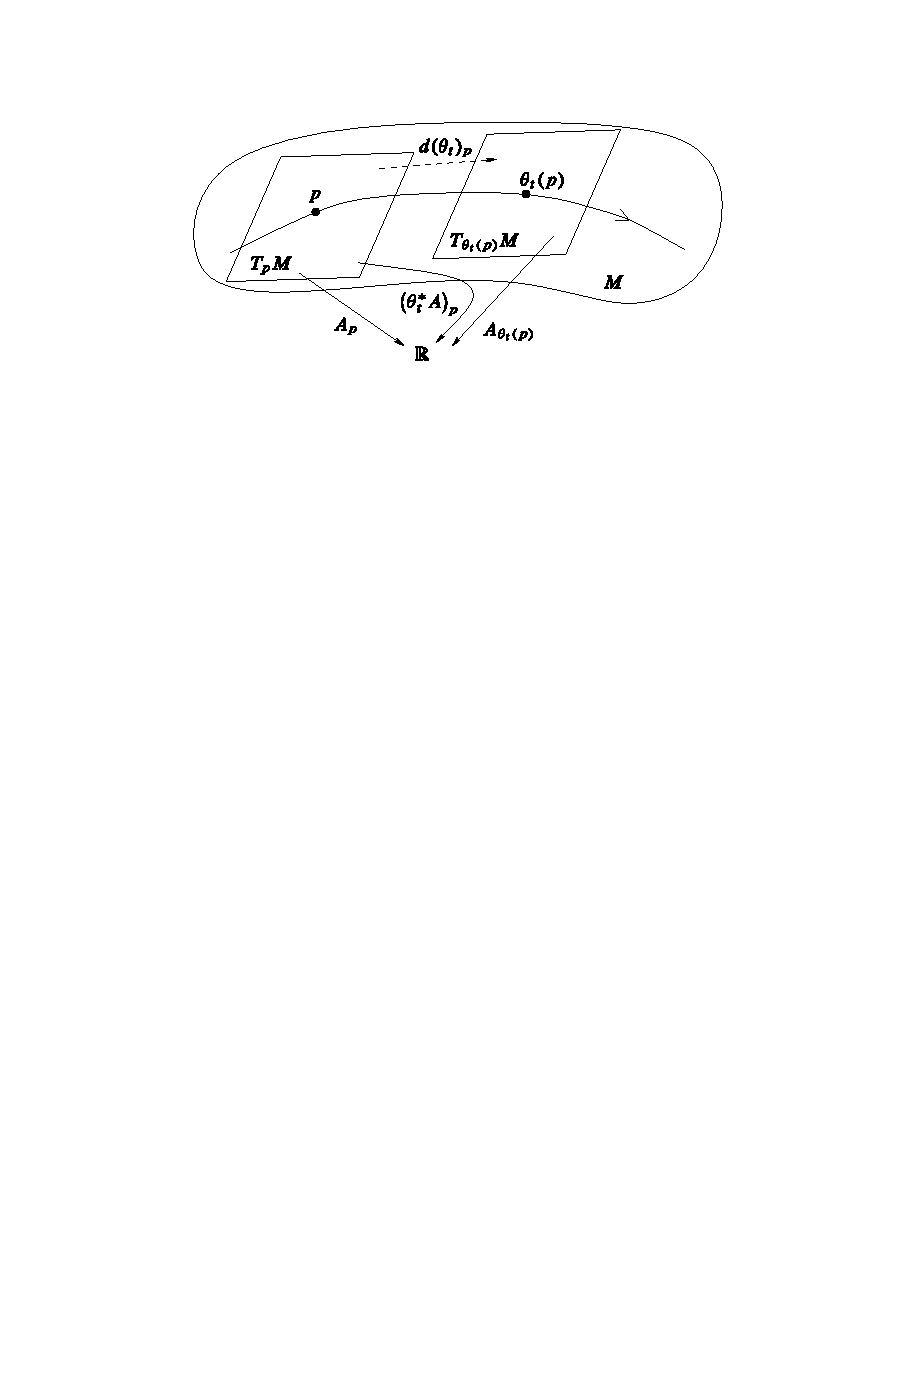
\includegraphics{pictures/Lie-derivative-tensor}
\caption{The Lie derivative of a tensor field.}
\end{figure}
\begin{lemma}
With $M,V$, and $A$ as above, the derivative $(\mathfrak{L}_VA)_p$ exists for every $p\in M$ and defines $\mathfrak{L}_VA$ as a smooth tensor field on $M$.
\end{lemma}
\begin{proposition}\label{tensor Lie derivative prop}
Let $M$ be a smooth manifold and let $V\in\X(M)$. Suppose $f$ is a smooth real-valued function $($regarded as a $0$-tensor field$)$ on $M$, and $A,B$ are smooth covariant tensor fields on $M$.
\begin{itemize}
\item[(a)] $\mathfrak{L}_Vf=Vf$.
\item[(b)] $\mathfrak{L}_V(fA)=(Vf)A+f\mathfrak{L}_VA$.
\item[(c)] $\mathfrak{L}_V(A\otimes B)=(\mathfrak{L}_VA)\otimes B+A\otimes(\mathfrak{L}_VB)$.
\item[(d)] If $X_1,\dots,X_k$ are smooth vector fields and $A$ is a smooth $k$-tensor field,
\begin{align*}
\mathfrak{L}_V\big(A(X_1,\dots,X_k)\big)=(\mathfrak{L}_VA)(X_1,\dots,X_k)+\sum_{i=1}^{k}A(X_1,\dots,\mathfrak{L}_VX_i,\dots,X_k)
\end{align*}
\end{itemize}
\end{proposition}
\begin{proof}
Let $\theta$ be the flow of $V$. For a real-valued function $f$, we can write
\[\theta^*_tf(p)=(f\circ\theta_t)(p)=f\circ\theta^{(p)}(t)\]
Thus the definition of $\mathfrak{L}_Vf$ reduces to the ordinary derivative with respect to $t$ of the composite function $f\circ\theta^{(p)}(t)$. Because $\theta^{(p)}(t)$ is an integral curve of $V$, it follows from Proposition~\ref{diff function curve} that
\[(\mathfrak{L}_Vf)_p=\frac{d}{dt}\Big|_{t=0}f\circ\theta^{(p)}=df_p\big(\dot{\theta}^{(p)}(0)\big)=df_p(V_p)=Vf(p)\]
This proves (a).\par
The other assertions can be proved by the technique we used in Theorem~\ref{Lie derivative bracket}: in a neighborhood of a regular point for $V$, if $(u^i)$ are coordinates in which $V=\partial/\partial u^1$, then it follows immediately from the definition that $\mathfrak{L}_V$ acts on a tensor field simply by taking the partial derivative of its coefficients with respect to $u^1$, and (b)--(d) all follow from the ordinary product rule. The same relations hold on the support of $V$ by continuity, and on the complement of the support because the flow of $V$ is trivial there.
\end{proof}
One consequence of this proposition is the following formula expressing the Lie
derivative of any smooth covariant tensor field in terms of Lie brackets and ordinary
directional derivatives of functions, which allows us to compute Lie derivatives
without first determining the flow.
\begin{corollary}\label{Lie derivative tensor}
If $V$ is a smooth vector field and $A$ is a smooth covariant $k$-tensor field, then for any smooth vector fields $X_1,\dots,X_k$,
\begin{align}\label{Lie derivative tensor-1}
(\mathfrak{L}_VA)(X_1,\dots,X_k)=V\big(A(X_1,\dots,X_k)\big)-\sum_{i=1}^{k}A(X_1,\dots,[V,X_i],\dots,X_k).
\end{align}
\end{corollary}
\begin{proof}
From Proposition~\ref{tensor Lie derivative prop}(d) we have
\[(\mathfrak{L}_VA)(X_1,\dots,X_k)=\mathfrak{L}_V(A(X_1,\dots,X_k))-\sum_{i=1}^{k}A(X_1,\dots,\mathfrak{L}_VX_i,\dots,X_k).\]
Replace $\mathfrak{L}_V(A(X_1,\dots,X_k))$ by $V\big(A(X_1,\dots,X_k)\big)$ and $\mathfrak{L}_VX_i$ by $[V,X_i]$, we get the claim.
\end{proof}
\begin{corollary}\label{covector Lie diff}
If $f\in C^\infty(M)$, then $\mathfrak{L}_V(df)=d(\mathfrak{L}_Vf)$.
\end{corollary}
\begin{proof}
Using $(\ref{Lie derivative tensor-1})$, for any $X\in\X(M)$ we compute
\begin{align*}
(\mathfrak{L}_Vdf)(X)&=V\big(df(X)\big)-df([V,X])=VXf-(VX-XV)f\\
&=XVf=X(\mathfrak{L}_Vf)=d(\mathfrak{L}_Vf)(X),
\end{align*}
thus the claim follows.
\end{proof}
One drawback of formula $(\ref{Lie derivative tensor-1})$ is that in order to calculate what $\mathfrak{L}_VA$ does to vectors $v_1,\dots,v_k$ at a point $p\in M$, one must first extend them to vector fields in a neighborhood of $p$. But Corollary~\ref{covector Lie diff} lead to an easy method for computing Lie derivatives of smooth tensor fields in coordinates that avoids this problem, since any tensor field can be written locally as a linear combination of functions multiplied by tensor products of exact $1$-forms. The next example illustrates the technique.
\begin{example}
Suppose $A$ is an arbitrary smooth covariant $2$-tensor field, and $V$ is a smooth vector field. We compute the Lie derivative $\mathfrak{L}_VA$ in smooth local coordinates $(x^i)$. First, we observe that \[\mathfrak{L}_Vdx^i=d(\mathfrak{L}_Vx^i)=d(Vx^i)=dV^i.\] 
Therefore,
\begin{align*}
\mathfrak{L}_VA&=\mathfrak{L}_V(A_{ij}\,dx^i\otimes dx^j)\\
&=\mathfrak{L}_V(A_{ij})\,dx^i\otimes dx^j+A_{ij}\mathfrak{L}_V(dx^i\otimes dx^j)\\
&=VA_{ij}\,dx^i\otimes dx^j+A_{ij}\mathfrak{L}_V(dx^i)\otimes dx^j+A_{ij}\,dx^i\otimes\mathfrak{L}_V(dx^j)\\
&=VA_{ij}\,dx^i\otimes dx^j+A_{ij}\,dV^i\otimes dx^j+A_{ij}\,dx^i\otimes dV^j\\
&=VA_{ij}\,dx^i\otimes dx^j+A_{ij}\frac{\partial V^i}{\partial x^k}\,dx^k\otimes dx^j+A_{ij}\frac{\partial V^j}{\partial x^k}\,dx^i\otimes dx^k\\
&=\Big(VA_{ij}+A_{kj}\frac{\partial V^k}{\partial x^i}+A_{ik}\frac{\partial V^k}{\partial x^j}\Big)dx^i\otimes dx^j.
\end{align*}
\end{example}
Recall that the Lie derivative of a vector field $W$ with respect to $V$ is zero if and
only if $W$ is invariant under the flow of $V$ (see Theorem~\ref{vector field commute iff}). It turns out that the Lie derivative of a covariant tensor field has exactly the same interpretation. If $A$ is a smooth tensor field on $M$ and $\theta$ is a flow on $M$, we say that $A$ is \textbf{invariant under $\bm{\theta}$} if for each $t$, the map $\theta_t$ pulls $A$ back to itself wherever it is defined; more precisely, this means
\[d(\theta_t)_p^*(A_{\theta_t(p)})=A_p\]
for all $(t,p)$ in the domain of $\theta$. If $\theta$ is a global flow, this is equivalent to $\theta_t^*A=A$ for all $t\in\R$.\par
In order to prove the connection between Lie derivatives and invariance under flows, we need the following proposition, which shows how the Lie derivative can be used to compute $t$-derivatives at times other than $t=0$. It is a generalization to tensor fields of Proposition~\ref{Lie derivative t_0}.
\begin{proposition}\label{Lie der tensor t_0}
Suppose $M$ is a smooth manifold with or without boundary and $V\in\X(M)$. If $\partial M\neq\emp$, assume in addition that $V$ is tangent to $\partial M$. Let $\theta$ be the
flow of $V$. For any smooth covariant tensor field $A$ and any $(t_0,p)$ in the domain
of $\theta$,
\[\frac{d}{dt}\Big|_{t=t_0}(\theta_t^*A)_p=\big(\theta_{t_0}^*(\mathfrak{L}_VA)\big)_p\]
\end{proposition}
\begin{proof}
After expanding the definitions of the pullbacks, we see that we have to prove
\[\frac{d}{dt}\Big|_{t=0}d(\theta_t)_p^*(A_{\theta_t(p)})=d(\theta_{t_0})_p^*\big((\mathfrak{L}_VA)_{\theta_{t_0}(p)}\big)\]
Just as in the proof of Proposition~\ref{Lie derivative t_0}, the change of variables $t=s+t_0$ yields
\begin{align*}
&\frac{d}{dt}\Big|_{t=0}d(\theta_t)_p^*(A_{\theta_t(p)})=\frac{d}{ds}\Big|_{s=0}d(\theta_{s+t_0})_p^*(A_{\theta_{s+t_0}(p)})=\frac{d}{ds}\Big|_{s=0}d(\theta_{t_0})_p^*\circ d(\theta_{s})_{\theta_{t_0}(p)}^*(A_{\theta_{s}(\theta_{t_0}(p))})\\
&=d(\theta_{t_0})_p^*\frac{d}{ds}\Big|_{s=0}d(\theta_{s})_{\theta_{t_0}(p)}^*(A_{\theta_{s}(\theta_{t_0}(p))})=d(\theta_{t_0})_p^*\big((\mathfrak{L}_VA)_{\theta_{t_0}(p)}\big).
\end{align*}
\end{proof}
\begin{theorem}\label{tensor filed invariant flow iff}
Let $M$ be a smooth manifold and let $V\in\X(M)$. A smooth covariant tensor field $A$ is invariant under the flow of $V$ if and only if $\mathfrak{L}_VA=0$.
\end{theorem}
\begin{proof}
This follows from the definition of $\mathfrak{L}_VA$.
\end{proof}
\subsection{Exercise}
\begin{exercise}
Let $M$ be a smooth $n$-manifold, and let $A$ be a smooth covariant $k$-tensor field on $M$. If $(U,(x^i))$ and $(\widetilde{U},(\widetilde{x}^j))$ are overlapping smooth charts on $M$, we can write
\[A=A_{i_1\dots i_k}dx^{i_1}\otimes\cdots\otimes dx^{i_k}=\widetilde{A}_{j_1\dots j_k}d\widetilde{x}^{j_1}\otimes\cdots\otimes d\widetilde{x}^{j_k}.\]
Compute the transformation law.
\end{exercise}
\begin{proof}
Recall the formulas
\[ d\widetilde{x}^j=\frac{\partial\widetilde{x}^j}{\partial x^i}dx^i.\]
Thus
\[A=\widetilde{A}_{j_1\dots j_k}d\widetilde{x}^{j_1}\otimes\cdots\otimes d\widetilde{x}^{j_k}=\widetilde{A}_{j_1\dots j_k}\frac{\partial\widetilde{x}^{j_1}}{\partial x^{i_1}}\cdots\frac{\partial\widetilde{x}^{j_k}}{\partial x^{i_k}}dx^{i_1}\otimes\cdots\otimes dx^{i_k}.\]
This gives the claim.
\end{proof}
\begin{exercise}\label{tensor field Lie derivative bracket}
Suppose $M$ is a smooth manifold, $A$ is a smooth covariant tensor field on $M$, and $V,W\in\X(M)$. Show that
\[\mathfrak{L}_V\mathfrak{L}_WA-\mathfrak{L}_W\mathfrak{L}_VA=\mathfrak{L}_{[V,W]}A.\]
\end{exercise}
\begin{proof}
Let $X_1,\dots,X_k\in\X(M)$, then
\begin{align*}
&(\mathfrak{L}_V\mathfrak{L}_WA)(X_1,\dots,X_k)=V\big(\mathfrak{L}_WA(X_1,\dots,X_k)\big)-\sum_{i=1}^{k}\mathfrak{L}_WA(X_1,\dots,[V,X_i],\dots,X_k)\\
&=VW\big(A(X_1,\dots,X_k)\big)-\sum_{i=1}^{k}V\big(A(X_1,\dots,[W,X_i],\dots,X_k)\big)\\
&-\sum_{i=1}^{k}W\big(A(X_1,\dots,[V,X_i],\dots,X_k)\big)+\sum_{i\neq j}A(X_1,\dots,[W,X_i],\dots,[V,X_j],\dots,X_k)\\
&+\sum_{i=1}^{k}A\big(X_1,\dots,\big[W,[V,X_i]\big],\dots,X_k\big).
\end{align*}
And thus
\begin{align*}
&(\mathfrak{L}_V\mathfrak{L}_WA)(X_1,\dots,X_k)-(\mathfrak{L}_W\mathfrak{L}_VA)(X_1,\dots,X_k)=(VW-WV)\big(A(X_1,\dots,X_k)\big)\\
&\quad+\sum_{i=1}^{k}A\big(X_1,\dots,\big[W,[V,X_i]\big],\dots,X_k\big)-\sum_{i=1}^{k}A\big(X_1,\dots,\big[V,[W,X_i]\big],\dots,X_k\big).
\end{align*}
Therefore, we compute using the Jacobi identity
\begin{align*}
&(\mathfrak{L}_{[V,W]}A)(X_1,\dots,X_k)=(VW-WV)(A(X_1,\dots,X_k))-\sum_{i=1}^{k}A(X_1,\dots,\big[[V,W],X_i\big],\dots,X_k)\\
&=(VW-WV)(A(X_1,\dots,X_k))+\sum_{i=1}^{k}A(X_1,\dots,\big[[W,X_i],V\big]+\big[[X_i,V],W\big],\dots,X_k)\\
&=(VW-WV)(A(X_1,\dots,X_k))+\sum_{i=1}^{k}A(X_1,\dots,\big[W,[V,X_i]\big]-\big[[V,W],X_i\big],\dots,X_k)\\
&=(\mathfrak{L}_V\mathfrak{L}_WA)(X_1,\dots,X_k)-(\mathfrak{L}_W\mathfrak{L}_VA)(X_1,\dots,X_k).
\end{align*}
\end{proof}
\begin{exercise}
Let $M$ be a smooth manifold and $V\in\X(M)$. Show that the Lie derivative operators on covariant tensor fields, $\mathfrak{L}_V:\mathcal{T}^k(M)\to\mathcal{T}^k(M)$ for $k\geq 0$, are uniquely characterized by the following properties:
\begin{itemize}
\item[(a)] $\mathfrak{L}_V$ is linear over $\R$.
\item[(b)] $\mathfrak{L}_Vf=Vf$ for $f\in\mathcal{T}^0(M)=C^\infty(M)$. 
\item[(c)] $\mathfrak{L}_V(A\otimes B)=\mathfrak{L}_VA\otimes B+A\otimes\mathfrak{L}_VB$ for $A\in\mathcal{T}^k(M)$ and $B\in\mathcal{T}^l(M)$.
\item[(d)] $\mathfrak{L}_V(\omega(X))=(\mathfrak{L}_V\omega)(X)+\omega([V,X])$ for $\omega\in\mathcal{T}^1(M),X\in\X(M)$.
\end{itemize}
\end{exercise}
\begin{proof}
Let $\mathfrak{L}$ be an operator satisfying (a)--(d), we prove that $\mathfrak{L}=\mathfrak{L}_V$.
\begin{itemize}
\item First, by (b) and (d) we have for $\omega\in\mathcal{T}^1(M),X\in\X(M)$:
\[(\mathfrak{L}\omega)(X)=V(\omega(X))-\omega([V,X])=(\mathfrak{L}_V\omega)(X)\]
\item Then, by induction, we can prove
\[\mathfrak{L}(\omega_1\otimes\cdots\otimes \omega_k)=\mathfrak{L}_V(\omega_1\otimes\cdots\otimes\omega_k).\]
\item By taking local charts, we verify that $\mathfrak{L}=\mathfrak{L}_V$.
\end{itemize}
\end{proof}
\section{Riemannian metrics}
\subsection{Riemannian manifolds}
The most important examples of symmetric tensors on a vector space are inner products. Any inner product allows us to define lengths of vectors and angles between
them, and thus to do Euclidean geometry.\par
Transferring these ideas to manifolds, we obtain one of the most important applications
of tensors to differential geometry. Let $M$ be a smooth manifold with or without boundary. A \textbf{Riemannian metric} on $M$ is a smooth symmetric covariant $2$-tensor field on $M$ that is positive definite at each point. A \textbf{Riemannian manifold} is a pair $(M,g)$, where $M$ is a smooth manifold and $g$ is a Riemannian metric on $M$. One sometimes simply says $M$ is a Riemannian manifold if $M$ is understood to be endowed with a specific Riemannian metric. A Riemannian manifold with boundary is defined similarly.\par
If $g$ is a Riemannian metric on $M$, then for each $p\in M$, the $2$-tensor $g_p$ is an
inner product on $T_pM$. Because of this, we often use the notation $\langle v,w\rangle_g$ to denote the real number $g_p(v,w)$ for $v,w\in T_pM$.\par
In any smooth local coordinates $(x^i)$, a Riemannian metric can be written
\[g=g_{ij}\,dx^i\otimes dx^j,\]
where $(g_{ij})$ is a symmetric positive definite matrix of smooth functions. The symmetry of $g$ allows us to write $g$ also in terms of symmetric products as follows:
\begin{align*}
g=&g_{ij}\,dx^i\otimes dx^j=\frac{1}{2}(g_{ij}\,dx^i\otimes dx^j+g_{ji}\,dx^j\otimes dx^i)=\frac{1}{2}g_{ij}(dx^i\otimes dx^j+dx^j\otimes dx^i)=g_{ij}\,dx^idx^j.
\end{align*}
\begin{example}[\textbf{The Euclidean Metric}]
The simplest example of a Riemannian metric is the Euclidean metric $\widebar{g}$ on $\R^n$, given in standard coordinates by
\[\widebar{g}=\delta_{ij}\,dx^i\otimes dx^j.\]
It is common to abbreviate the symmetric product of a tensor $\alpha$ with itself by $\alpha^2$, so the Euclidean metric can also be written
\[\widebar{g}=(dx^1)^2+\cdots+(dx^n)^2.\]
\end{example}
\begin{example}[\textbf{Product Metrics}]
If $(M,g)$ and $(\widetilde{M},\widetilde{g})$ are Riemannian manifolds, we can define a Riemannian metric $\widehat{g}=g\oplus\widetilde{g}$ on the product manifold $M\times\widetilde{M}$, called the product metric, as follows:
\[\widehat{g}\big((v,\widetilde{v}),(w,\widetilde{w})\big)=g(v,w)+\widetilde{g}(\widetilde{v},\widetilde{w})\]
for any $(v,\widetilde{v}),(w,\widetilde{w})\in T_pM\oplus T_q\widetilde{M}$. Given any local coordinates $(x^1,\dots,x^n)$ for $M$ and $(y^1,\dots,y^m)$ for $\widetilde{M}$, we obtain local coordinates $(x^1,\dots,x^n,y^1,\dots,y^m)$ for $M\times\widetilde{M}$, and the product metric is represented locally by the block diagonal matrix
\[(\widehat{g}_{ij})=\begin{pmatrix}
g_{ij}&0\\
0&\widetilde{g}_{ij}
\end{pmatrix}\]
\end{example}
\begin{proposition}[\textbf{Existence of Riemannian Metrics}]
Every smooth manifold with or without boundary admits a Riemannian metric.
\end{proposition}
\begin{proof}
Let $M$ be a smooth manifold with or without boundary, and choose a covering of $M$ by smooth coordinate charts $(U_\alpha,\varphi_\alpha)$. In each coordinate domain, there
is a Riemannian metric $g_\alpha=\varphi_\alpha^*\widebar{g}$, whose coordinate expression is $\delta_{ij}\,dx^idx^j$. Let $\{\psi_\alpha\}$ be a smooth partition of unity subordinate to the cover $\{U_\alpha\}$, and define
\[g=\sum_\alpha\psi_\alpha g_\alpha,\]
with each term interpreted to be zero outside $\supp(\psi_\alpha)$. By local finiteness, there are only finitely many nonzero terms in a neighborhood of each point, so this expression defines a smooth tensor field. It is obviously symmetric, so only positivity needs to be checked. If $v\in T_pM$ is any nonzero vector, then
\[g_p(v,v)=\sum_\alpha\psi_\alpha(p)g_\alpha|_p(v,v).\]
This sum is nonnegative, because each term is nonnegative. At least one of the functions
$\psi_\alpha$ is strictly positive at $p$. Because $g_\alpha|_p(v,v)>0$, it follows that $g_p(v,v)>0$.
\end{proof}
Below are just a few of the geometric constructions that can be defined on a Riemannian manifold $(M,g)$ with or without boundary.
\begin{itemize}
\item The length or norm of a tangent vector $v\in T_pM$ is defined to be
\[|v|_g=\langle v,v\rangle_g^{1/2}=g_p(v,v)^{1/2}\]
\item The angle between two nonzero tangent vectors $v,w\in T_pM$ is the unique  $\theta\in[0,\pi]$ satisfying
\[\cos\theta=\frac{\langle v,w\rangle_g}{|v|_g|w|_g}\]
\item Tangent vectors $v,w\in T_pM$ are said to be orthogonal if $\langle v,w\rangle_g=0$. This means either one or both vectors are zero, or the angle between them is $\pi/2$.
\end{itemize}
One highly useful tool for the study of Riemannian manifolds is orthonormal frames. Let $(M,g)$ be an $n$-dimensional Riemannian manifold with or without 
boundary. Just as we did for the case of $\R^n$ in Section~\ref{vector field section}, we say a local frame $(E_1,\dots,E_n)$ for $M$ on an open subset 
$U\sub M$ is an \textbf{orthonormal frame} if the vectors $(E_1|_p,\dots,E_n|_p)$ form an orthonormal basis for $TpM$ at each point $p\in U$, or 
equivalently if $\langle E_i,E_j\rangle_g=\delta_{ij}$, in which case $g$ has the local expression
\[g=(\eps^1)^2+\cdots+(\eps^n)^2.\]
where $(\eps^i)^2$ denotes the symmetric product $(\eps^i)^2=\eps^i\otimes\eps^i$.
\begin{example}
The coordinate frame $(\partial/\partial x^i)$ is a global orthonormal frame for $\R^n$
with the Euclidean metric.
\end{example}
\begin{example}
The frame $(E_1,E_2)$ on $\R^2-\{0\}$ defined in Example~\ref{polar frame R^2} is a local orthonormal frame for $\R^2$. As we observed in Example~\ref{commute frame eg}, it is not a coordinate frame in any coordinates.
\end{example}
The next proposition is proved in just the same way as Lemma~\ref{Gram-Schmidt frame}, with the Euclidean dot product replaced by the inner product $\langle\cdot,\cdot\rangle_g$.
\begin{proposition}\label{Gram Schmidt Riemannian}
Suppose $(M,g)$ is a Riemannian manifold with or without boundary, and 
$(X_j)$ is a smooth local frame for $M$ over an open subset $U\sub M$. 
Then there is a smooth orthonormal frame $(E_j)$ over $U$ such that 
$\mathrm{span}(E_1|_p,\dots,E_j|_p)=\mathrm{span}(X_1|_p,\dots,X_j|_p)$ for each $1\leq j\leq n$ and each $p\in U$.
\end{proposition}
\begin{proof}
Applying the Gram–Schmidt algorithm to the vectors $(X_1|_p,\dots,X_n|_p)$ at each $p\in U$, we obtain an ordered $n$-tuple of rough orthonormal vector fields 
$(E_1,\dots,E_n)$ over $U$ satisfying the span conditions. Because the vectors whose norms appear in the denominators of the Gram–Schmidt formulas are nowhere 
vanishing, it follows that each vector field $E_j$ is smooth. The last statement of the proposition follows by applying this construction to any smooth local frame in a neighborhood of $p$. 
In particular, for every $p\in M$, there is a smooth orthonormal frame $(E_j)$ defined on some neighborhood of $p$.
\end{proof}
\begin{corollary}[\textbf{Existence of Local Orthonormal Frames}]\label{orthonormal frame exist}
Let $(M,g)$ be a Riemannian manifold with or without boundary. For each $p\in M$, there is a smooth orthonormal frame on a neighborhood of $p$.
\end{corollary}
Observe that Corollary~\ref{orthonormal frame exist} does not show that there are smooth coordinates on a neighborhood of $p$ for which the \textit{coordinate frame} is 
orthonormal. In fact, this is possible only when the metric is flat, that is, locally isometric to the Euclidean metric.\par
For a Riemannian manifold $(M,g)$ with or without boundary, we define the unit tangent bundle to be the subset $UTM\sub TM$ consisting of unit vectors:
\[UTM=\{(p,v)\in TM:|v|_g=1\}\]
\begin{proposition}[\textbf{Properties of the Unit Tangent Bundle}]
If $(M,g)$ is a Riemannian manifold with or without boundary, its unit tangent bundle $UTM$ is a smooth, properly embedded codimension-$1$ submanifold with 
boundary in $TM$, with $\partial(UTM)=\pi^{-1}(\partial M)$ (where $\pi:UTM\to M$ is the canonical projection). The unit tangent bundle is connected if and only if $M$ 
is connected when $n>1$, and compact if and only if $M$ is compact.
\end{proposition}
\begin{proof}
By the local orthonormal frames, we can replace $M$ by $\R^n$. If $U$ is open in $\R^n$, then the unit tangent bundle is diffeomorphic to $U\times S^{n-1}$, and therefore has codimension $1$. It is properly embedded since $S^{n-1}$ 
is properly embedded in $\R^n$. Similarly, if $U$ is a half ball in $\H^n$, we can see that the tangent bundle is diffeomorphic to $U\times S^{n-1}$, and therefore has boundary charts. 
This also proves that $\partial(UTM)=\pi^{-1}(\partial M)$.\par
For the last claim, note that the projection $\pi:UTM\to M$ is surjective and open (Proposition~\ref{smooth subm prop}), so $M$ is connect if $UTM$ is, and compact if $UTM$ is. Now we show the converse.\par
If $M$ is compact, then for any $p\in M$ we can find a comapct subset $V_p$ such that the interior of $V_p$ is open and the tangent bundle of $V_p$ is 
trivial. Then we can find 
$p_1,\dots,p_n\in M$ such that $M\sub\bigcup_{i=1}^{n}\Int(V_{p_i})$, and so 
\[UTM=\bigcup_{i=1}^{n}\pi^{-1}(\Int(V_{p_i}))\sub\bigcup_{i=1}^{n}\pi^{-1}(V_{p_i}).\]
Since the tangent bundle of $V_{p_i}$ is trivial, we have $\pi^{-1}(V_{p_i})=V_{p_i}\times S^{n-1}$. This implies that $UTM$ is compact since it is the union of 
finitely many compact subsets, so it is compact.\par
If $M$ is connected and $n>1$, then the fiber of $UTM$ is diffeomorphic to $S^{n-1}$ and so it connected. Assume that $UTM=U\cup V$ for two disjoint open subsets, then 
$M=\pi(E)=\pi(U)\cup\pi(V)$ is the union of the open subsets $\pi(U)$ and $\pi(V)$ wich are not disjoint since $M$ is connected. Let $p\in\pi(U)\cap\pi(V)$, then there 
exists $v_1\in U$, $v_2\in V$ such that $\pi(v_1)=\pi(v_2)=p$. This means $E_p\cap U\neq\emp$ and $E_p\cap V\neq\emp$, so $E_p\cap U$ and $E_p\cap V$ is a partition of $E_p$. 
But $E_p$ is connected, this is a contradiction.
\end{proof}
\subsection{Methods for constructing riemannian metrics}
\subsubsection{Pullback metrics}
Suppose $M,N$ are smooth manifolds with or without boundary, $g$ is a Riemannian metric on $N$, and $F:M\to N$ is smooth. The pullback $F^*g$ is a smooth $2$-tensor field on $M$. If it is positive definite, it is a Riemannian metric on $M$, called the pullback metric determined by $F$. The next proposition shows when this is the
case.
\begin{proposition}[\textbf{Pullback Metric Criterion}]
Suppose $F:M\to N$ is a smooth map and $g$ is a Riemannian metric on $N$. Then $F^*g$ is a Riemannian metric on $M$ if and only if $F$ is a smooth immersion.
\end{proposition}
\begin{proof}
$F^*g$ is a Riemannian metric if and only if for all $p\in M$, $F^*g(v,v)=0$ implies $v=0$ for $v\in T_pM$, wich means $dF_p(v)=0$ implies $v=0$ for any $v\in T_pM$, which 
is to say $F$ is a immersion.
\end{proof}
If the coordinate representation for an immersion is known, then the pullback metric is easy to compute using the usual algorithm for computing pullbacks.
\begin{example}
Consider the smooth map $F:\R^2\to\R^3$ given by
\[F(u,v)=(u\cos v,u\sin v,v)\]
It is a proper injective smooth immersion, and thus it is an embedding by Proposition~\ref{smooth embedd if}. The pullback metric $F^*\widebar{g}$ can be computed by substituting the coordinate functions for $F$ in place of $x,y,z$ in the formula for $\widebar{g}$:
\begin{align*}
F^*\widebar{g}&=(du\cos v)^2+(du\sin v)^2+(dv)^2\\
&=(\cos v\,du-u\sin v\,dv)^2+(\sin v\,du+u\cos v\,dv)^2+dv^2\\
&=du^2+u^2\,dv^2+dv^2=(u^2+1)^2\,du^2+dv^2.
\end{align*}
By convention, when $u$ is a real-valued function, the notation $du^2$ means the symmetric product $dudu$, not $d(u^2)$.
\end{example}
To transform a Riemannian metric under a change of coordinates, we use the
same technique as we used for covector fields: think of the change of coordinates as the identity map expressed in terms of different coordinates for the domain and
codomain, and use the formula of Corollary~\ref{tensor pullback formula}.
\begin{example}\label{Riemann metric polar}
To illustrate, we compute the coordinate expression for the Euclidean metric $\widebar{g}=dx^2+dy^2$ on $\R^2$ in polar coordinates. Substituting $x=r\cos\theta$ and $y=r\sin\theta$ and expanding, we obtain
\begin{align*}
\widebar{g}&=dx^2+dy^2=[d(r\cos\theta)]^2+[d(r\sin\theta)]^2\\
&=(\cos\theta\,dr-r\sin\theta\,d\theta)^2+(\sin\theta\,dr+r\cos\theta\,d\theta)^2\\
&=dr^2+r^2\,d\theta^2
\end{align*}
\end{example}
If $(M,g)$ and $(\widetilde{M},\widetilde{g})$ are both Riemannian manifolds, a smooth map 
$F:M\to\widetilde{M}$ is called a \textbf{Riemannian isometry} if it is a diffeomorphism 
that satisfies $F^*\widetilde{g}=g$. More generally, $F$ is called a \textbf{local isometry} 
if every point $p\in M$ has a neighborhood $U$ such that $F|_U$ is an isometry of $U$ 
onto an open subset of $\widetilde{M}$, or equivalently, if $F$ is a local diffeomorphism 
satisfying $F^*\widetilde{g}=g$.\par
If there exists a Riemannian isometry between $(M,g)$ and $(\widetilde{M},\widetilde{g})$, 
we say that they are \textbf{isometric} as Riemannian manifolds. If 
each point of $M$ has a neighborhood that is isometric to an open subset of 
$(\widetilde{M},\widetilde{g})$, then we say that $(M,g)$ is \textbf{locally isometric} 
to $(\widetilde{M},\widetilde{g})$.\par
One such property is flatness. A Riemannian $n$-manifold $(M,g)$ is said to be a 
\textbf{flat Riemannian manifold}, and $g$ is a \textbf{flat metric}, if $(M,g)$ 
is locally isometric to $(\R^n,\widebar{g})$.
\begin{proposition}
Suppose $(M,g)$ and $(\widetilde{M},\widetilde{g})$ are isometric Riemannian manifolds, then $g$ is flat if and only if $\widetilde{g}$ is flat.
\end{proposition}
The next theorem is the key to deciding whether a Riemannian metric is flat.
\begin{theorem}\label{Riemann flat iff}
For a Riemannian manifold $(M,g)$, the following are equivalent:
\begin{itemize}
\item[(a)] $g$ is flat.
\item[(b)] Each point of $M$ is contained in the domain of a smooth coordinate chart in which $g$ has the coordinate representation $g=\delta_{ij}dx^idx^j$.
\item[(c)] Each point of $M$ is contained in the domain of a smooth coordinate chart in which the coordinate frame is orthonormal.
\item[(d)] Each point of $M$ is contained in the domain of a commuting orthonormal frame.
\end{itemize}
\end{theorem}
\begin{proof}
The implications $(a)\Rightarrow(b)\Rightarrow(c)\Rightarrow(d)$ are easy consequences of the definitions. The remaining implication, $(d)\Rightarrow(a)$, follows from the canonical form theorem for commuting frames: if $(E_i)$ is a commuting orthonormal frame for $g$ on an open subset $V\sub M$, then Theorem~\ref{flow commute canonical form} implies that each $p\in V$ is contained in the domain of a smooth chart $(U,\varphi)$ in which the coordinate frame is equal to $(E_i)$. This means $\varphi_*E_i=\partial/\partial x^i$, so the diffeomorphism $\varphi:U\to\varphi(U)$ satisfies
\[\varphi^*\widebar{g}(E_i,E_j)=\widebar{g}(\varphi_*E_i,\varphi_*E_j)=\widebar{g}\Big(\frac{\partial}{\partial x^i},\frac{\partial}{\partial x^j}\Big)=\delta_{ij}=g(E_i,E_j)\]
Bilinearity then shows that $\varphi^*\widebar{g}=g$, so $\varphi$ is an isometry between $(U,\varphi|_U)$ and $\varphi(U)$ with the Euclidean metric. This shows that $g$ is flat.
\end{proof}
\subsubsection{Riemannian submanifolds}
Pullback metrics are especially important for submanifolds. If $(M,g)$ is a Riemannian
manifold with or without boundary, every submanifold $S\sub M$ (immersed or embedded, with or without boundary) automatically inherits a pullback metric $\iota^*g$, where $\iota:S\hookrightarrow M$ is inclusion. In this setting, the pullback metric is also called the \textbf{induced metric} on $S$. By definition, this means for $v,w\in T_pS$ that
\[(\iota^*g)(v,w)=g(d\iota_p(v),d\iota_p(w))=g(v,w)\]
because $d\iota_p:T_pS\to T_pM$ is our usual identification of $T_pS$ as a subspace of $T_pM$. Thus $\iota^*g$ is just the restriction of $g$ to pairs of vectors tangent to $S$. With this metric, $S$ is called a \textbf{Riemannian submanifold} (with or without boundary) of $M$.
\begin{example}
The metric $\mathring{g}=\iota^*\widebar{g}$ induced on $S^n$ by the usual inclusion $\iota:S^n\hookrightarrow\R^{n+1}$ is called the \textbf{round metric} or the \textbf{standard metric} on the sphere.
\end{example}
The next lemma describes one of the most important tools for studying Riemannian submanifolds. If 
$(\widetilde{M},\widetilde{g})$ is an $m$-dimensional smooth Riemannian manifold and $(M,g)$ is 
an $n$-dimensional submanifold (both with or without boundary), a local frame $(E_1,\dots,E_m)$ for 
$\widetilde{M}$ on an open subset $\widetilde{U}\sub\widetilde{M}$ is said to be \textbf{adapted to $\bm{M}$} if 
the first $n$ vector fields $(E_1,\dots,E_n)$ are tangent to $M$. In case $\widetilde{M}$ has empty
boundary (so that slice coordinates are available), adapted local orthonormal frames are easy to find.
\begin{proposition}[\textbf{Existence of Adapted Orthonormal Frames}]\label{Riemann embed adapted}
Let $(\widetilde{M},\widetilde{g})$ be a Riemannian manifold (without boundary), and let $(M,g)$ be 
an embedded smooth submanifold with or without boundary. Given $p\in M$, there exist a neighborhood 
$\widetilde{U}$ of $p$ in $\widetilde{M}$ and a smooth orthonormal frame for $\widetilde{M}$ on 
$\widetilde{U}$ that is adapted to $M$.
\end{proposition}
\begin{proof}
We can find a slice chart at $p$ for $M$, and use the Gram-Schmidt algorithm to a coordinate frame in slice 
coordinates to produce a orthonormal frame. By the span property, we see that this frame is adapted to $M$.
\end{proof}
Suppose $(\widetilde{M},\widetilde{g})$ is a Riemannian manifold and $(M,g)$ is a smooth submanifold 
with or without boundary in $\widetilde{M}$. Given $p\in M$, a vector $v\in T_p\widetilde{M}$ is said to be
\textbf{normal to $\bm{M}$} if $\langle v,w\rangle=0$ for every $w\in T_pM$. The space of all vectors 
normal to $M$ at $p$ is a subspace of $T_p\widetilde{M}$, called the \textbf{normal space at $\bm{p}$} and 
denoted by $N_pM=(T_pM)^{\bot}$. At each $p\in M$, the ambient tangent space $T_p\widetilde{M}$ splits as an 
orthogonal direct sum $T_p\widetilde{M}=T_pM\oplus N_pM$. A section $N$ of the ambient tangent bundle 
$T\widetilde{M}|_{M}$ is called a \textbf{normal vector field along $\bm{M}$} if $N_p\in N_pM$ for each $p\in M$. The set
\[NM=\coprod_{p\in M}N_pM\]
is called the normal bundle of $M$.
\begin{proposition}[\textbf{The Normal Bundle to a Riemannian Submanifold}]\label{Riemann normal bundle}
If $\widetilde{M}$ is a Riemannian $m$-manifold and $M$ is an immersed or embedded $n$-dimensional 
submanifold with or without boundary, then $NM$ is a smooth rank-$(m-n)$ vector subbundle of the ambient 
tangent bundle $T\widetilde{M}|_M$. There are smooth bundle homomorphisms
\[\pi^{\top}:T\widetilde{M}|_M\to TM,\quad \pi^{\bot}:T\widetilde{M}|_M\to NM\]
called the \textbf{tangential} and \textbf{normal projections}, that for each $p\in M$ restrict to
orthogonal projections from $T_p\widetilde{M}$ to $T_pM$ and $N_pM$, respectively.
\end{proposition}
\begin{proof}
Given any point $p\in M$, Theorem~\ref{immerse local embedd} shows that there is a neighborhood 
$U$ of $p$ in $M$ that is embedded in $\widetilde{M}$, and then Proposition~\ref{Riemann embed adapted} 
shows that there is a smooth orthonormal frame $(E_1,\dots,E_m)$ that is adapted to $U$ on some 
neighborhood $\widetilde{U}$ of $p$ in $\widetilde{M}$. This means that the restrictions of 
$(E_1,\dots,E_n)$ to $\widetilde{U}\cap U$ form a local orthonormal frame for $M$. Given such an 
adapted frame, the restrictions of the last $m-n$ vector fields $(E_{n+1},\dots,E_m)$ to $M$ form 
a smooth local frame for $NM$, so it follows from Lemma~\ref{vector subbundle crit} that $NM$ is a 
smooth subbundle.\par
The bundle homomorphisms $\pi^{\top}$ and $\pi^{\bot}$ are defined pointwise as orthogonal 
projections onto the tangent and normal spaces, respectively, which shows that they are uniquely 
defined. In terms of an adapted orthonormal frame, they can be written
\[\pi^{\top}(X^iE_i)=X^1E_1+\cdots+X^nE_n,\quad \pi^{\bot}(X^iE_i)=X^{n+1}E_{n+1}+\cdots+X^mE_m,\]
which shows that they are smooth.
\end{proof}
In case $\widetilde{M}$ is a manifold with boundary, the preceding constructions do not always work, 
because there is not a fully general construction of slice coordinates in that case. However, there 
is a satisfactory result in case the submanifold is the boundary itself, using boundary coordinates 
in place of slice coordinates.\par
Suppose $(M,g)$ is a Riemannian manifold with boundary. We will always consider $\partial M$ to be a 
Riemannian submanifold with the induced metric.
\begin{proposition}[\textbf{Existence of Outward-Pointing Normal}]\label{Riemann outward normal}
If $(M,g)$ is a smooth Riemannian manifold with boundary, the normal bundle to $\partial M$ is a 
smooth rank-$1$ vector bundle over $\partial M$, and there is a unique smooth outward-pointing unit 
normal vector field along all of $\partial M$. By this, we see that $N(\partial M)$ is a rank-$1$ 
vector subbundle of $TM|_{\partial M}$.
\end{proposition}
\begin{proof}
We can always construct a global smooth outward-pointing vector field by taking $-\partial/\partial x^n$ 
in boundary coordinates in a neighborhood of each boundary point, and gluing together with a partition 
of unity. By the Gram-Schmidt process, we may assume that this vector field is normal to $\partial M$.
\end{proof}
Computations on a submanifold $M\sub\widetilde{M}$ are usually carried out most conveniently in terms of 
a \textbf{smooth local parametrization}: this is a smooth map $X:U\to\widetilde{M}$, where $U$ is an open 
subset of $\R^n$ (or $\H^n$ in case $M$ has a boundary), such that $X(U)$ is an open subset of $M$, and such 
that $X$, regarded as a map from $U$ into $M$, is a diffeomorphism onto its image. Note that we can think of 
$X$ either as a map into $M$ or as a map into $\widetilde{M}$, both maps are typically denoted by the same 
symbol $X$. If we put $V=X(U)\sub\widetilde{M}$ and $\varphi=X^{-1}:V\to U$, then $(V,\varphi)$ is a smooth 
coordinate chart on $M$.
Suppose $(M,g)$ is a Riemannian submanifold of $(\widetilde{M},\widetilde{g})$ and $X:U\to\widetilde{M}$ is a
smooth local parametrization of $M$. The coordinate representation of $g$ in these coordinates is given by 
the following $2$-tensor field on $U$:
\[\varphi_*g=X^*g=X^*\iota^*\widetilde{g}=(\iota\circ X)^*\widetilde{g}.\]
Since $\iota\circ X$ is just the map $X$ itself, regarded as a map into $\widetilde{M}$, this is really just 
$X^*\widetilde{g}$. The simplicity of the formula for the pullback of a tensor field makes this expression
exceedingly easy to compute, once a coordinate expression for $\widetilde{g}$ is known. For example, if $M$ is 
an immersed $n$-dimensional Riemannian submanifold of $\R^m$ and $X:U\to\R^m$ is a smooth local parametrization 
of $M$, the induced metric on $U$ is just
\[g=X^*\widebar{g}=\sum_{i=1}^{m}(dX^i)^2=\sum_{i=1}^{m}\Big(\sum_{j=1}^{n}\frac{\partial X^i}{\partial u^j}du^j\Big)^2=\sum_{i=1}^{m}\sum_{j,k=1}^{n}\frac{\partial X^i}{\partial u^i}\frac{\partial X^i}{\partial u^k}du^jdu^k.\]
\begin{example}[\textbf{Induced Metrics in Graph Coordinates}]
Let $U\sub\R^n$ be an open subset, and let $S\sub\R^{n+1}$ be the graph of a smooth function $f:U\to\R$. The 
map $X:U\to\R^{n+1}$ given by $X(u^1,\dots,u^n)=(u^1,\dots,u^n,f(u))$ is a smooth global parametrization of 
$S$ and the induced metric on $S$ is given in graph coordinates by
\[X^*\widebar{g}=X^*\big((dx^1)^2+\cdots+(dx^{n+1})^2\big)=(du^1)^2+\cdots+(du^n)^2+(df)^2\]
For example, the upper hemisphere of $S^2$ is parametrized by the map $X:\B^2\to\R^3$ given by
\[X(u,v)=(u,v,\sqrt{1-u^2-v^2})\]
In these coordinates, the round metric can be written
\[\mathring{g}=X^*\widebar{g}=du^2+dv^2+\Big(\frac{u\,du+v\,dv}{\sqrt{1-u^2-v^2}}\Big)^2=\frac{(1-v^2)\,du^2+(1-u^2)\,dv^2+2uv\,dudv}{1-u^2-v^2}.\]
\end{example}
\begin{example}[\textbf{Induced Metrics on Surfaces of Revolution}]\label{surfaces of revolution induced metric}
Let $C$ be an embedded one dimensional submanifold of the half-plane $\{(r,z):r>0\}$ and let $S_C$ 
be the surface of revolution generated by $C$ as described in Example~\ref{surfaces of revolution}. To compute 
the induced metric on $S_C$, choose any smooth local parametrization $\gamma(t)=(a(t),b(t))$ for $C$, and note 
that the map $X(t,\theta)=(a(t)\cos\theta,a(t)\sin\theta,b(t))$ yields a smooth local parametrization of $S_C$, 
provided that $(t,\theta)$ is restricted to a sufficiently small open subset of the plane. Thus we can compute
\begin{align*}
X^*\widebar{g}&=\big(da(t)\cos\theta\big)^2+\big(da(t)\sin\theta\big)^2+\big(db(t)\big)^2\\
&=\big(a'(t)\cos\theta\,dt-a(t)\sin\theta\,d\theta\big)^2+\big(a'(t)\sin\theta\,dt+a(t)\cos\theta\,d\theta\big)^2+\big(b'(t)\,dt\big)^2\\
&=\big(a'(t)^2+b'(t)^2\big)dt^2+a(t)^2d\theta^2
\end{align*}
In particular, if $\gamma$ is a unit-speed curve, meaning that $|\gamma'(t)|^2=1$, this reduces to the simple formula $dt^2+a(t)^2d\theta^2$.\par
Here are some familiar examples of surfaces of revolution.
\begin{itemize}
\item[(a)] The embedded torus is the surface of revolution generated by the circle $(r-2)^2+z^2=1$. 
Using the unit-speed parametrization $\gamma(t)=(2+\cos t+\sin t)$ for the circle, we obtain the formula 
$dt^2+(2+\cos\theta)^2d\theta^2$ for the induced metric.
\item[(b)] The unit sphere $($minus the north and south poles$)$ is a surface of revolution whose 
generating curve is the semicircle parametrized by $\gamma(t)=(\sin t,\cos t)$ for $0<t<\pi$. The 
induced metric is $dt^2+(\sin t)^2d\theta^2$.
\item[(c)] The unit cylinder $x^2+y^2=1$ is a surface of revolution whose generating curve is the 
vertical line parametrized by $\gamma(t)=(1,t)$ for $t\in\R$. The induced metric is $dt^2+d\theta^2$.
\end{itemize}
\end{example}
\begin{example}[\textbf{The $\bm{n}$-Torus as a Riemannian Submanifold}]
The smooth covering map $X:\R^n\to T^n$ defined by $X(u^1,\cdots,u^n)=(\cos u^1,\sin u^1,\cdots,\cos u^n,\sin u^n)$ restricts to a 
smooth local parametrization on any sufficiently small open subset of $\R^n$, and the induced metric is 
\[X^*\widebar{g}=d(\cos u^1)^2+d(\sin u^1)^2+\cdots+d(\cos u^n)^2+d(\sin u^n)^2=(du^1)^2+\cdots+(du^n)^2.\]
Therefore the induced metric on $T^n$ is flat.
\end{example}
\subsubsection{Riemannian products}
Next we consider products. If $(M_1,g_1)$ and $(M_2,g_2)$ are Riemannian manifolds, the product manifold 
$M_1\times M_2$ has a natural Riemannian metric $g=g_1\oplus g_2$, called the product metric, defined by
\[g_{(p_1,p_2)}((v_1,v_2),(w_1,w_2))=g_1|_{p_1}(v_1,w_1)+g_2|_{p_2}(v_2,w_2).\]
where $(v_1,v_2)$ and $(w_1,w_2)$ are elements of $T_{p_1}M_1\oplus T_{p_2}M_2$, which is naturally 
identified with $T_{(p_1,p_2)}(M_1\times M_2)$. Smooth local coordinates $(x^1,\dots,x^n)$ for $M_1$ and 
$(x^{n+1},\dots,x^{n+m})$ for $M_2$ give coordinates $(x^1,\dots,x^{n+m})$ for $M_1\oplus M_2$. In terms 
of these coordinates, the product metric has the local expression $g=g_{ij}dx^idx^j$, where $(g_{ij})$ is 
the block diagonal matrix
\[(g_{ij})=\begin{pmatrix}
(g_1)&0\\
0&(g_2)
\end{pmatrix}\]
Product metrics on products of three or more Riemannian manifolds are defined similarly.\par
Here is an important generalization of product metrics. Suppose $(M_1,g_1)$ and $(M_2,g_2)$ are two 
Riemannian manifolds, and $f:M_1\to\R^+$ is a strictly positive smooth function. The \textbf{warped product} 
$M_1\times_f M_2$ is the product manifold $M_1\times M_2$ endowed with the Riemannian metric $g=g_1\oplus f^2g_2$, 
defined by
\[g_{(p_1,p_2)}((v_1,v_2),(w_1,w_2))=g_1|_{p_1}(v_1,w_1)+f(p_1)^2g_2|_{p_2}(v_2,w_2).\]
where $(v_1,v_2),(w_1,w_2)\in T_{p_1}M_1\oplus T_{p_2}M_2$ as before. A wide variety of metrics can be constructed in this way; here are just a few examples.
\begin{example}\label{Riemann metric R^n in polar}
If we let $\rho$ denote the standard coordinate function on $\R^+\sub\R$, then the map 
$\varPhi(\rho,\omega)=\rho\omega$ gives an isometry from the warped product $\R^+\times_{\rho}S^{n-1}$ 
to $\R^n\setminus\{0\}$ with its Euclidean metric. To see this, we use the parametrization
\[X:(\rho,x^1,\dots,x^{n-1})\mapsto(\rho,x^1,\dots,x^{n-1},\sqrt{1-|x|^2})\]
of $\R^+\times S^{n-1}$ to compute the pull back metric $\varPhi^*\widebar{g}$ as follows:
\begin{align*}
&(\varPhi\circ X)^*\widebar{g}=d(\rho x^1)^2+\cdots+d(\rho x^{n-1})^2+d(\rho\sqrt{1-|x|^2})^2\\
&=(x^1\,d\rho+\rho\,dx^1)^2+\cdots+(x^{n-1}\,d\rho+\rho\,dx^{n-1})^2+\Big(\sqrt{1-|x|^2}d\rho-\rho\frac{x^1dx^1+\cdots+x^{n-1}dx^{n-1}}{\sqrt{1-|x|^2}}\Big)^2\\
&=d\rho^2+\rho^2((dx^1)^2+\cdots+(dx^{n-1})^2)+\rho^2\frac{(x^1dx^1+\cdots+x^{n-1}dx^{n-1})^2}{1-|x|}\\
&\quad+2\rho(x^1dx^1d\rho+\cdots+x^{n-1}dx^{n-1}d\rho)-2\rho(x^1dx^1d\rho+\cdots+x^{n-1}dx^{n-1}d\rho)\\
&=d\rho^2+\rho^2\Big((dx^1)^2+\cdots+(dx^{n-1})^2+\frac{(x^1dx^1+\cdots+x^{n-1}dx^{n-1})^2}{1-|x|}\Big)\\
&=d\rho^2+\rho^2\mathring{g}
\end{align*}
\end{example}
\begin{example}
Every surface of revolution can be expressed as a warped product, as follows. Let 
$H$ be the half-plane $\{(r,z):r>0\}$, let $C\sub H$ be an embedded smooth $1$-dimensional submanifold, 
and let $S_C\sub\R^3$ denote the corresponding surface of revolution as in 
Example~\ref{surfaces of revolution induced metric}. Endow $C$ with the Riemannian metric induced from 
the Euclidean metric on $H$, and let $S^1$ be endowed with its standard metric. Let $f:C\to\R$ be the 
distance to the $z$-axis: $f(r,z)=r$. Then from Example~\ref{surfaces of revolution induced metric} we 
see that $S_C$ is isometric to the warped product $C\times_f S^1$.
\end{example}
\subsubsection{Riemannian submersions}
Unlike submanifolds and products of Riemannian manifolds, which automatically inherit 
Riemannian metrics of their own, quotients of Riemannian manifolds inherit Riemannian 
metrics only under very special circumstances. Now we see what those circumstances 
are.\par
Suppose $\widetilde{M}$ and $M$ are smooth manifolds, $\pi:\widetilde{M}\to M$ is a 
smooth submersion, and $\widetilde{g}$ is a Riemannian metric on $\widetilde{M}$. By 
the submersion level set theorem, each fiber $\widetilde{M}_y=\pi^{-1}(y)$ is a properly 
embedded smooth submanifold of $\widetilde{M}$. At each point $x\in\widetilde{M}$, we 
define two subspaces of the tangent space $T_x\widetilde{M}$ as follows: the 
\textbf{vertical tangent space} at $x$ is
\[V_x=\ker d\pi_x=T_x(\widetilde{M}_{\pi(x)})\]
(that is, the tangent space to the fiber containing $x$), and the \textbf{horizontal tangent 
space} at $x$ is its orthogonal complement:
\[H_x=(V_x)^\bot\]
Then the tangent space $T_x\widetilde{M}$ decomposes as an orthogonal direct sum 
$T_x\widetilde{M}=H_x\oplus V_x$. Note that the vertical space is well defined for 
every submersion, because it does not refer to the metric; but the horizontal 
space depends on the metric.\par
A vector field on $\widetilde{M}$ is said to be a \textbf{horizontal vector field} if its 
value at each point lies in the horizontal space at that point; a \textbf{vertical vector 
field} is defined similarly. Given a vector field $X$ on $M$, a vector field $\widetilde{X}$ 
on $\widetilde{M}$ is called a \textbf{horizontal lift} of $X$ if $\widetilde{X}$ is 
horizontal and $\pi$-related to $X$.\par
The next proposition is the principal tool for doing computations on Riemannian 
submersions.
\begin{proposition}[\textbf{Properties of Horizontal Vector Fields}]\label{Riemann horizontal vector field}
Let $\widetilde{M}$ and $M$ be smooth manifolds, let $\pi:\widetilde{M}\to M$ be a 
smooth submersion, and let $\widetilde{g}$ be a Riemannian metric on $\widetilde{M}$.
\begin{itemize}
\item[(a)] Every smooth vector field $W$ on $\widetilde{M}$ can be expressed 
uniquely in the form $W=W^H+W^V$, where $W^H$ is horizontal, $W^V$ is vertical, 
and both $W^H$ and $W^V$ are smooth.
\item[(b)] Every smooth vector field on $M$ has a unique smooth horizontal lift 
to $\widetilde{M}$.
\item[(c)] For every $x\in\widetilde{M}$ and $v\in H_x$, there is a vector field $X\in\X(M)$ 
whose horizontal lift $\widetilde{X}$ satisfies $\widetilde{X}_x=v$.
\end{itemize}
\end{proposition}
\begin{proof}
Let $p\in\widetilde{M}$ be arbitrary. Because $\pi$ is a smooth submersion, the rank 
theorem shows that there exist smooth coordinate charts $(\widetilde{U},(x^i))$ 
centered at $p$ and $(U,(y^j))$ centered at $\pi(x)$ in which $\pi$ has the 
coordinate representation
\[\pi(x^1,\dots,x^n,x^{n+1},\dots,x^{m})=(x^1,\dots,x^n)\]
where $m=\dim\widetilde{M}$ and $n=\dim M$. It follows that at each point $q\in\widetilde{U}$, 
the vertical space $V_q$ is spanned by the vectors $(\partial/\partial x^{n+1}|_q,\dots,\partial/\partial x^{m}|_q)$. 
(It probably will not be the case, however, that the horizontal space is 
spanned by the other $n$ basis vectors.) If we apply the Gram–Schmidt algorithm 
to the ordered frame $(\partial/\partial x^{n+1}|,\dots,\partial/\partial x^{m},\partial/\partial x^1,\dots,\partial/\partial x^n)$, 
we obtain a smooth orthonormal frame $(E_1,\dots,E_m)$ on $\widetilde{U}$ 
such that $V_q$ is spanned by $(E_1|_q,\dots,E_{m-n}|_q)$ at each $q\in\widetilde{U}$. It follows that $H_q$ 
is spanned by $(E_{n-m+1}|_q,\dots,E_{m}|_q)$.\par
Now let $W\in\X(\widetilde{M})$ be arbitrary. At each point $q\in\widetilde{M}$, $W_q$ 
can be written uniquely as a sum of a vertical vector plus a horizontal vector, 
thus defining a decomposition $W=W^V+W^H$ into rough vertical and horizontal 
vector fields. To see that they are smooth, just note that in a neighborhood 
of each point we can express $W$ in terms of a frame $(E_1,\dots,E_m)$ of the 
type constructed above as $W=W^1E_1+\cdots+W^mE_m$ with smooth coefficients $(W^i)$, 
and then it follows that
\[W^V=W^1E_1+\cdots+W^{m-n}E_{m-n},\quad W^H=W^{n-m+1}E_{n-m+1}+\cdots+W^mE_{m},\]
both of which are smooth.\par
Let $X\in\X(M)$ be arbitrary. By the coordinate representation constructed above, we see that 
$d\pi$ is just the projection onto $H_q$, which is spanned by $(E_{m-n+1},\dots,E_m)$. Therefore 
we can use $X$ to define a rough horizontal vector field on $\widetilde{M}$. From the 
local coordinate presentation we see that $\widetilde{X}$ is smooth.\par
For every $x\in\widetilde{M}$ and $v\in H_x$, we can choose coordinates as above, and construct a 
vector field on $M$ such that $X_{\pi(x)}=d\pi(v)$. Then by the construction above 
the horizontal lift $\widetilde{X}$ satisfies $\widetilde{X}_x=v$.
\end{proof}
The fact that every horizontal vector at a point of $\widetilde{M}$ can be extended 
to a horizontal lift on all of $\widetilde{M}$ (part (c) of the preceding 
proposition) is highly useful for computations. It is important to be aware, 
though, that not every horizontal vector field on $\widetilde{M}$ is a horizontal 
lift, as the next example shows.
\begin{example}
Let $\pi:\R^2\to\R$ be the projection map $\pi(x,y)=yx$, and let $W$ be the smooth vector 
field $y\partial/\partial x$ on $\R^2$. Then $W$ is horizontal, but there is no 
vector field on $\R$ whose horizontal lift is equal to $W$.
\end{example}
Now we can identify some quotients of Riemannian manifolds that inherit metrics 
of their own. Let us begin by describing what such a metric should look like. 
Suppose $(\widetilde{M},\widetilde{g})$ and $(M,g)$ are Riemannian manifolds, 
and $\pi:\widetilde{M}\to M$ is a smooth submersion. Then $\pi$ is said to be 
a \textbf{Riemannian submersion} if for each $x\in\widetilde{M}$, the differential 
$d\pi_x$ restricts to a linear isometry from $H_x$ onto $T_{\pi(x)}M$. In other 
words, $\widetilde{g}_x(v,w)=g_{\pi(x)}(d\pi_x(v),d\pi_x(w))$ whenever $v,w\in H_x$.
\begin{example}[\textbf{Riemannian Submersions}]
\mbox{}
\begin{itemize}
\item[(a)] The projection $\pi:\R^{n+k}\to\R^n$ onto the first $n$ coordinates is 
a Riemannian submersion if $\R^{n+k}$ and $\R^n$ are both endowed with their 
Euclidean metrics.
\item[(b)] If $M$ and $N$ are Riemannian manifolds and $M\times N$ is endowed 
with the product metric, then both projections $\pi_M:M\times N\to M$ and $\pi_N:M\times N\to N$ 
are Riemannian submersions.
\item[(c)] If $M\times_fN$ is a warped product manifold, then the projection $\pi_M:M\times_fN\to M$ 
is a Riemannian submersion, but $\pi_N$ typically is not.
\end{itemize}
\end{example}
Given a Riemannian manifold $(\widetilde{M},\widetilde{g})$ and a surjective 
submersion $\pi:\widetilde{M}\to M$, it is almost never the case that there is 
a metric on $M$ that makes $\pi$ into a Riemannian submersion. It is not hard 
to see why: for this to be the case, whenever $p_1,p_2\in\widetilde{M}$ are two points in 
the same fiber $\pi^{-1}(y)$, the linear maps $(d\pi_{p_i}|_{H_{p_i}})^{-1}:T_yM\to H_{p_i}$ 
both have to pull $\widetilde{g}$ back to the same inner product on $T_yM$.
There is, however, an important special case in which there is such a metric. Suppose 
$\pi:\widetilde{M}\to M$ is a smooth surjective submersion, and $G$ is a group 
acting on $\widetilde{M}$. We say that the action is \textbf{vertical} if every 
element $\varphi\in G$ takes each fiber to itself, meaning that $\pi(\varphi\cdot p)=\pi(p)$ 
for all $p\in M$. The action is \textbf{transitive on fibers} if for each $p,q\in M$ 
such that $\pi(p)=\pi(q)$, there exists $\varphi\in G$ such that $\varphi\cdot p=q$.
If in addition $\widetilde{M}$ is endowed with a Riemannian metric, the action 
is said to be an \textbf{isometric action} or an \textbf{action by isometries}, 
and the metric is said to be \textbf{invariant under $\bm{G}$}, if the map $x\mapsto\varphi\cdot x$ 
is an isometry for each $\varphi\in G$. In that case, provided the action is 
effective (so that different elements of $G$ define different isometries of $\widetilde{M}$), 
we can identify $G$ with a subgroup of $\Iso(\widetilde{M},g)$. Since an isometry 
is, in particular, a diffeomorphism, every isometric action is an action by diffeomorphisms.
\begin{theorem}\label{Riemann submersion induce metric}
Let $(\widetilde{M},\widetilde{g})$ be a Riemannian manifold, let $\pi:\widetilde{M}\to M$ 
be a surjective smooth submersion, and let $G$ be a group acting on $\widetilde{M}$. 
If the action is isometric, vertical, and transitive on fibers, then there is a 
unique Riemannian metric on $M$ such that $\pi$ is a Riemannian submersion.
\end{theorem}
The next corollary describes one important situation to which the preceding theorem
applies.
\begin{corollary}\label{Riemann orbit space induce metric}
Suppose $(\widetilde{M},\widetilde{g})$ is a Riemannian manifold, and $G$ is a Lie 
group acting smoothly, freely, properly, and isometrically on $\widetilde{M}$. Then 
the orbit space $M=\widetilde{M}/G$ has a unique smooth manifold structure and 
Riemannian metric such that $\pi:\widetilde{M}\to M$ is a Riemannian submersion.
\end{corollary}
\begin{proof}
Under the given hypotheses, the quotient manifold theorem shows that $M$ has a 
unique smooth manifold structure such that the quotient map $\widetilde{M}\to\widetilde{M}/G$ 
is a smooth submersion. It follows easily from the definitions in that case that 
the given action of $G$ on $\widetilde{M}$ is vertical and transitive on fibers. 
Since the action is also isometric, Theorem~\ref{Riemann submersion induce metric} shows that $M$ inherits a 
unique Riemannian metric making $\pi$ into a Riemannian submersion.
\end{proof}
Here is an important example of a Riemannian metric defined in this way.
\begin{example}[\textbf{The Fubini-Study Metric}]
Let $n$ be a positive integer, and consider the complex projective space $\CP^n$. The 
map $\pi:\C^{n+1}\setminus\{0\}\to\CP^n$ sending each point in $\C^{n+!}\setminus\{0\}$ 
to its span is a surjective smooth submersion. Identifying $\C^{n+1}$ with $\R^{2n+2}$ 
endowed with its Euclidean metric, we can view the unit sphere $S^{2n+1}$ with 
its round metric $\mathring{g}$ as an embedded Riemannian submanifold of $\C^{n+1}\setminus\{0\}$. 
Let $p:S^{2n+1}\to\CP^n$ denote the restriction of the map $\pi$. Then $p$ is 
smooth, and it is surjective, because every $1$-dimensional complex subspace 
contains elements of unit norm. We need to show that it is a submersion. Let $z_0\in S^{2n+1}$ 
and set  $\zeta_0=p(z_0)\in\CP^n$. Since $\pi$ is a smooth submersion, it has a 
smooth local section $\sigma:U\to\C^{n+1}\setminus\{0\}$ defined on a neighborhood 
$U$ of $\zeta_0$. Let $\widetilde{\sigma}$ be the radial projection of $\sigma$ 
onto the sphere: $\widetilde{\sigma}=\sigma/|\sigma|$. Then $\widetilde{\sigma}$ is a 
local section of $p$. By Theorem~\ref{submersion iff local section} we see that $p$ 
is a submersion.\par
Define an action of $S^1$ on $S^{2n+1}$ by complex multiplication
\[\lambda\cdot(z^1,\dots,z^{n+1})=(\lambda z^1,\dots,\lambda z^{n+1})\]
for $\lambda\in S^1$ (viewed as a complex number of norm $1$) and $(z^1,\dots,z^{n+1})\in S^{2n+1}$. 
This is easily seen to be isometric, vertical, and transitive on fibers of $p$. By 
Theorem~\ref{Riemann submersion induce metric}, therefore, there is a unique 
metric on $\CP^n$ such that the map $p:S^{2n+1}\to\CP^n$ is a Riemannian submersion. 
This metric is called the \textbf{Fubini-Study metric}.
\end{example}
\subsubsection{Riemannian coverings}
Another important special case of Riemannian submersions occurs in the context of
covering maps. Suppose $(\widetilde{M},\widetilde{g})$ and $(M,g)$ are Riemannian 
manifolds. A smooth covering map $\pi:\widetilde{M}\to M$ is called a \textbf{Riemannian 
covering} if it is a local isometry.
\begin{proposition}\label{Riemann cover induce metric}
Suppose $\pi:\widetilde{M}\to M$ is a smooth normal covering map, and $\widetilde{g}$ 
is any metric on $\widetilde{M}$ that is invariant under all covering automorphisms. 
Then there is a unique metric $g$ on $M$ such that $\pi$ is a Riemannian covering.
\end{proposition}
\begin{proof}
Proposition~\ref{smooth cover prop} shows that $\pi$ is a surjective smooth 
submersion. The automorphism group acts vertically by definition, and we know 
that it acts transitively on fibers when the covering is normal. It then follows 
from Theorem~\ref{Riemann submersion induce metric} that there is a unique metric 
$g$ on $M$ such that $\pi$ is a Riemannian submersion. Since a Riemannian 
submersion is a local isometry, it follows that $\pi$ is a Riemannian covering.
\end{proof}
\begin{proposition}\label{Riemann discrete action induce metric}
Suppose $(\widetilde{M},\widetilde{g})$ is a Riemannian manifold, and $\Gamma$ is a 
discrete Lie group acting smoothly, freely, properly, and isometrically on $\widetilde{M}$. 
Then $\widetilde{M}/\Gamma$ has a unique Riemannian metric such that the quotient 
map $\pi:\widetilde{M}\to\widetilde{M}/\Gamma$ is a normal Riemannian covering.
\end{proposition}
\begin{proof}
Proposition~\ref{Lie discrete covering map} shows that $\pi$ is a smooth normal 
covering map, and Proposition~\ref{Riemann cover induce metric} shows that 
$\widetilde{M}/\Gamma$ has a unique Riemannian metric such that $\pi$ is a 
Riemannian covering.
\end{proof}
\begin{corollary}
Suppose $(\widetilde{M},\widetilde{g})$ and $(M,g)$ are connected Riemannian 
manifolds, $\pi:\widetilde{M}\to M$ is a normal Riemannian covering map, and $\Gamma=\Aut_{\pi}(\widetilde{M})$. 
Then $M$ is isometric to $\widetilde{M}/\Gamma$.
\end{corollary}
\begin{proof}
Proposition~\ref{Lie group coveing group discrete} shows that with the discrete 
topology, $\Gamma$ is a discrete Lie group acting smoothly, freely, and properly 
on $\widetilde{M}$, and then Proposition~\ref{Lie discrete covering map} shows 
that $\widetilde{M}/\Gamma$ is a smooth manifold and the quotient map $q:\widetilde{M}\to\widetilde{M}/\Gamma$ 
is a smooth normal covering map. The fact that both $\pi$ and $q$ are normal 
coverings implies that $\Gamma$ acts transitively on the fibers of both maps, so 
the two maps are constant on each other's fibers. Proposition~\ref{smooth quotient unique} 
then implies that there is a diffeomorphism $F:M\to\widetilde{M}/\Gamma$ that 
satisfies $q\circ F=\pi$. Because both $q$ and $\pi$ are local isometries, $F$ is 
too, and because it is bijective it is a global isometry.
\end{proof}
\begin{example}
The two-element group $\{\pm 1\}$ acts smoothly, freely, properly, and isometrically 
on $S^n$ by multiplication. We know that the quotient space is diffeomorphic to 
the real projective space $\RP^n$ and the quotient map $q:S^n\to\RP^n$ is a smooth 
normal covering map. Because the action is isometric, Proposition~\ref{Riemann discrete action induce metric} 
shows that there is a unique metric on $\RP^n$ such that $q$ is a Riemannian covering.
\end{example}
\begin{example}[\textbf{The Open M\"obius Band}]
The \textbf{open M\"obius band} is the quotient space $M=\R^2/\Z$, where $\Z$ acts on $\R^2$ by 
\[n\cdot(x,y)=(x+n,(-1)^ny).\]
This action is smooth, free, proper, and isometric, and therefore $M$ inherits a 
flat Riemannian metric such that the quotient map is a Riemannian covering.
\end{example}
\subsection{Basic constructions on Riemannian manifolds}
\subsubsection{Raising and lowering indices}
One elementary but important property of Riemannian metrics is that they allow us
to convert vectors to covectors and vice versa. Given a Riemannian metric $g$ on $M$,
we define a bundle homomorphism $\widehat{g}:TM\to T^*M$ by setting
\[\widehat{g}(v)(w)=g_p(v,w)\]
for each $p\in M$ and each $v,w\in T_pM$. To see that this is a smooth bundle 
homomorphism, it is easiest to consider its action on smooth vector fields:
\[\widehat{g}(X)(Y)=g(X,Y)\for X,Y\in\X(M).\]
Because $\widehat{g}(X)(Y)$ is linear over $C^\infty(M)$ as a function of $Y$, it 
follows from the tensor characterization lemma (Lemma~\ref{tensor field smooth crit}) 
that $\widehat{g}(X)$ is a smooth covector field, and because $\widehat{g}(X)$ is 
linear over $C^\infty(M)$ as a function of $X$, this defines $\widehat{g}$ as a 
smooth bundle homomorphism by the bundle homomorphism characterization lemma (Lemma~\ref{vector bundle homo char}). 
As usual, we use the same symbol for both the pointwise bundle homomorphism 
$\widehat{g}:TM\to T^*M$ and the linear map on sections $\widehat{g}:\X(M)\to\X^*(M)$.\par
Note that $\widehat{g}$ is injective at each point, because $\widehat{g}(v)=0$ 
for some $v\in T_pM$ implies
\[0=\widehat{g}(v)(v)=g(v,v)\]
which in turn implies $v=0$. For dimensional reasons, therefore, $\widehat{g}$ is 
bijective, so it is a bundle isomorphism (Proposition~\ref{vector bundle smooth iso iff bi}).\par
In any smooth coordinates $(x^i)$, we can write $g=g_{ij}dx^idx^j$. Thus, if $X$ 
and $Y$ are smooth vector fields, we have
\[\widehat{g}(X)(Y)=g_{ij}X^iY^j\]
which implies that the covector field $\widehat{g}(X)$ has the coordinate 
expression
\[\widehat{g}(X)=g_{ij}X^idx^j\]
In other words, $\widehat{g}$ is the bundle homomorphism whose matrix with respect 
to coordinate frames for $TM$ and $T^*M$ is the same as the matrix of $g$ itself.\par
It is customary to denote the components of the covector field $\widehat{g}(X)$ by
\[\widehat{g}=X_jdx^j,\quad\text{where }X_j=g_{ij}X^i.\]
Because of this, one says that $\widehat{g}(X)$ is obtained from $X$ by lowering 
an index. The notation $X^\flat$ is frequently used for $\widehat{g}(X)$, because 
the symbol $\flat$ is used in musical notation to indicate that a tone is to be 
lowered.\par
The matrix of the inverse map $\widehat{g}^{-1}:T^*M\to TM$ is thus the inverse 
of $(g_{ij})$. We let $(g^{ij})$ denote the matrix-valued 
function whose value at $p\in M$ is the inverse of the matrix $(g_{ij}(p))$, so 
that
\[g^{ij}g_{jk}=g_{kj}g^{ji}=\delta^i_k\]
Because $g_{ij}$ is a symmetric matrix, so is $g^{ij}$, as you can easily check. 
Thus for a covector field $\omega\in\X^*(M)$, the vector field 
$\widehat{g}^{-1}(\omega)$ has the coordinate representation
\[\widehat{g}^{-1}(\omega)=\omega^i\frac{\partial}{\partial x^i},\quad\text{where }\omega^i=\omega_ig^{ij}.\]
We use the notation $\sharp$ for $\widehat{g}^{-1}$, and say that $\omega^\sharp$ 
is obtained from $\omega$ by raising an index. Because the symbols $\flat$ and 
$\sharp$ are borrowed from musical notation, these two inverse isomorphisms are 
frequently called the \textbf{musical isomorphisms}. A handy mnemonic device for 
keeping the flat and sharp operations straight is to remember that the value of 
$\omega^\sharp$ at each point is a vector, which we visualize as a (sharp) arrow; 
while the value of $X^\flat$ is a covector, which we visualize by means of its 
(flat) level sets.\par
The most important use of the sharp operation is to reinstate the \textbf{gradient} as a 
vector field on Riemannian manifolds. For any smooth real-valued function $f$ on 
a Riemannian manifold $(M,g)$ with or without boundary, we define a vector field 
called the gradient of $f$ by
\[\grad f:=(df)^\sharp=\widehat{g}^{-1}(df).\]
Unraveling the definitions, we see that for any $X\in\X(M)$, the gradient satisfies
\[\langle\grad f,X\rangle_g=\widehat{g}(\grad f)(X)=df(X)=Xf.\]
Thus $\grad f$ is the unique vector field that satisfies
\[\langle\grad f,X\rangle_g=Xf\for X\in\X(M),\]
or equivalently,
\begin{align}\label{Riemann grad def}
\langle\grad f,\cdot\rangle_g=df.
\end{align}
In smooth coordinates, $\grad f$ has the expression
\[\grad f=g^{ij}\frac{\partial f}{\partial x^i}\frac{\partial}{\partial x^j}.\]
In particular, this shows that gradf is smooth. On Rn with the Euclidean metric,
this reduces to
\[\grad f=\delta^{ij}\frac{\partial f}{\partial x^i}\frac{\partial}{\partial x^j}=\sum_{i=1}^{n}\frac{\partial f}{\partial x^i}\frac{\partial}{\partial x^i}.\]
Thus our new definition of the gradient in this case coincides with the gradient from
elementary calculus. In other coordinates, however, the gradient does not generally
have the same form.
\begin{example}
Let us compute the gradient of a function $f\in C^\infty(\R^2)$ with respect to the Euclidean metric in polar coordinates. From Example~\ref{Riemann metric polar} we see that the matrix of $\widebar{g}$ in polar coordinates is $(\begin{smallmatrix}
1&0\\
0&r^2
\end{smallmatrix})$, so its inverse matrix is $(\begin{smallmatrix}
1&0\\
0&r^{-2}
\end{smallmatrix})$.
Inserting this into the formula for the gradient, we obtain
\[\grad f=\frac{\partial f}{\partial r}\frac{\partial}{\partial r}+\frac{1}{r^2}\frac{\partial f}{\partial\theta}\frac{\partial}{\partial\theta}.\]
\end{example}
The next proposition shows that the gradient has the same geometric interpretation
on a Riemannian manifold as it does in Euclidean space. If $f$ is a smooth
real-valued function on a smooth manifold $M$, recall that a point $p\in M$ is 
called a \textbf{regular point} of $f$ if $df_p\neq 0$, and a \textbf{critical point} of $f$ 
otherwise; and a level set $f^{-1}(c)$ is called a regular level set if every point of 
$f^{-1}(c)$ is a regular point of $f$. Corollary~\ref{subm level set} shows that 
each regular level set is an embedded smooth hypersurface in $M$.
\begin{proposition}
Suppose $(M,g)$ is a Riemannian manifold, $f\in C^{\infty}(M)$, and $\mathcal{R}\sub M$ 
is the set of regular points of $f$. For each $c\in\R$, the set $M_c=f^{-1}(c)\cap\mathcal{R}$, 
if nonempty, is an embedded smooth hypersurface in $M$, and $\grad f$ is everywhere 
normal to $M_c$.
\end{proposition}
\begin{proof}
From the definition of gradient we have
\[\langle\grad f|_p,v\rangle=df_p(v).\]
By Proposition~\ref{tangent space level set} we see that $T_pM_c=\ker df$, therefore the claim holds.
\end{proof}
The flat and sharp operators can be applied to tensors of any rank, in any 
index position, to convert tensors from covariant to contravariant or 
vice versa. Formally, this operation is defined as follows: if $F$ is any 
$(k,l)$-tensor and $i\in\{1,\dots,k+l\}$ is any covariant index position 
for $F$ (meaning that the $i$-th argument is a vector, not a covector), we 
can form a new tensor $F^{\sharp}$ of type $(k+1,l-1)$ by setting
\[F^\sharp(\alpha_1,\dots,\alpha_{k+l})=F(\alpha_1,\dots,\alpha_i^{\sharp},\dots,\alpha_{k+l})\]
whenever $\alpha_1,\dots,\alpha_{k+l}$ are vectors or covectors as appropriate. 
In any local frame, the components of $F^{\sharp}$ are obtained by multiplying 
the components of $F$ by $g^{kl}$ and contracting one of the indices of $g^{kl}$ 
with the $i$-th index of $F$. Similarly, if $i$ is a contravariant index 
position, we can define a $(k-1,l+1)$-tensor $F^{\flat}$ by
\[F^\flat(\alpha_1,\dots,\alpha_{k+l})=F(\alpha_1,\dots,\alpha_i^{\flat},\dots,\alpha_{k+l})\]
In components, it is computed by multiplying by $g_{kl}$ and contracting.\par
For example, if $A$ is a mixed $3$-tensor given in terms of a local frame by
\[A=A^{j}_{ik}\eps^i\otimes E_j\otimes\eps^k\]
we can lower its middle index to obtain a covariant $3$-tensor $A^{\flat}$ with
components
\[A_{ijk}=g_{jl}A_{ik}^{l}.\]
Another important application of the flat and sharp operators is to extend 
the trace operator to covariant tensors. If $h$ is any covariant $k$-tensor 
field on a Riemannian manifold with $k\geq 2$, we can raise one of its 
indices (say the last one for definiteness) and obtain a $(1,k-1)$-tensor $h^{\sharp}$. 
The trace of $h^{\sharp}$ is thus a well-defined covariant $(k-2)$-tensor 
field. We define the trace of $h$ with respect to $g$ as
\[\tr_gh=\tr(h^\sharp).\]
Sometimes we may wish to raise an index other than the last, or to take 
the trace on a pair of indices other than the last covariant and 
contravariant ones. In each such case, we will say in words what is meant.\par
The most important case is that of a covariant $2$-tensor field. In this case, 
$h^{\sharp}$ is a $(1,1)$-tensor field, which can equivalently be regarded 
as an endomorphism field, and $\tr_gh$ is just the ordinary trace of this 
endomorphism field. In terms of a basis, this is
\[\tr_gh=h^i_i=g^{ij}h_{ij}.\]
In particular, in an orthonormal frame this is the ordinary trace of the 
matrix $(h_{ij})$ (the sum of its diagonal entries); but if the frame is 
not orthonormal, then this trace is different from the ordinary trace.\par
If $g$ is a Riemannian metric on $M$ and $(E_i)$ is a local frame on $M$, there 
is a potential ambiguity about what the expression $(g^{ij})$ represents: 
we have defined it to mean the inverse matrix of $(g_{ij})$, but one could 
also interpret it as the components of the contravariant $2$-tensor field 
$g^{\sharp\sharp}$ obtained by raising both of the indices of $g$. But these 
two interpretations lead to the same result:
\[g^{\sharp\sharp}=g^{lk}g^{ki}g_{ij}=g^{lj},\]
so we do not distinguish them.
\subsubsection{Inner products of tensors}
A Riemannian metric yields, by definition, an inner product on tangent 
vectors at each point. Because of the musical isomorphisms between vectors 
and covectors, it is easy to carry the inner product over to covectors as 
well. Suppose $g$ is a Riemannian metric on $M$, and $x\in M$. We can define 
an inner product on the cotangent space $T^*_xM$ by
\[\langle\omega,\eta\rangle_g=\langle\omega^\sharp,\eta^{\sharp}\rangle_g\]
To see how to compute this, we just use the basis formula for the sharp operator, 
together with the relation $g_{kl}g^{ki}=g_{lk}g^{ki}=\delta_l^i$, to obtain
\begin{align*}
\langle\omega,\eta\rangle_g&=g_{kl}(g^{ki}\omega_i)(g^{lj}\eta_j)\\
&=\delta^i_lg^{lj}\omega_i\eta_j\\
&=g^{ij}\omega_j\eta_j
\end{align*}
In other words, the inner product on covectors is represented by the 
inverse matrix $(g^{ij})$. Using our conventions for raising and lowering 
indices, this can also be written
\[\langle\omega,\eta\rangle=\omega_i\eta^j=\omega^i\eta_j.\]
Now the following result is immediate from the definition.
\begin{proposition}
Let $(M,g)$ be a Riemannian manifold with or without boundary, let $(E_i)$ 
be a local frame for $M$, and let $(\eps^i)$ be its dual coframe. Then the 
following are equivalent:
\begin{itemize}
\item[(a)] $(E_i)$ is orthonormal.
\item[(b)] $(\eps^i)$ is orthonormal.
\item[(c)] $(\eps^i)^{\sharp}=E_i$ for each $i$. 
\end{itemize}
\end{proposition}
This construction can be extended to tensor bundles of any rank, as the 
following proposition shows. First a bit of terminology: if $E\to M$ is a 
smooth vector bundle, a \textbf{smooth fiber metric} on $E$ is an inner 
product on each fiber $E_p$ that varies smoothly, in the sense that for any 
(local) smooth sections $\sigma,\tau$ of $E$, the inner product $(\sigma,\tau)$ 
is a smooth function.
\begin{proposition}[\textbf{Inner Products of Tensors}]
Let $(M,g)$ be an $n$-dimensional Riemannian manifold with or without 
boundary. There is a unique smooth fiber metric on each tensor bundle 
$T^{(k,l)}TM$ with the property that if $\alpha_1,\dots,\alpha_{k+l}$, 
$\beta_1,\dots,\beta_{k+l}$ are vector or covector fields as appropriate, 
then
\begin{align}\label{Riemann tensor inner prod-1}
\langle\alpha_1\otimes\cdots\otimes\alpha_{k+l},\beta_1\otimes\cdots\otimes\beta_{k+l}\rangle=\langle\alpha_{1},\beta_1\rangle\cdots\langle\alpha_{k+l},\beta_{k+l}\rangle.
\end{align}
With this inner product, if $(E_1,\dots,E_n)$ is a local orthonormal frame 
for $TM$ and $(\eps^1,\dots,\eps^n)$ is the corresponding dual coframe, 
then the collection of tensor fields $E_{i_1}\otimes\cdots\otimes E_{i_k}\otimes\eps^{j_1}\otimes\cdots\otimes\eps^{j_l}$ 
as all the indices range from $1$ to $n$ forms a local orthonormal frame 
for $T^{(k,l)}(T_pM)$. In terms of any (not necessarily orthonormal) frame, 
this fiber metric satisfies
\begin{align}\label{Riemann tensor inner prod-2}
\langle F,G\rangle=g_{i_1r_1}\cdots g_{i_kr_k}g^{j_1s_1}\cdots g^{j_ls_l}F^{i_1\dots i_k}_{j_1\dots j_l}G^{r_1\dots r_k}_{s_1\dots s_l}.
\end{align}
If $F$ and $G$ are both covariant, this can be written
\[\langle F,G\rangle=F_{j_1\dots j_l}G^{j_1\dots j_l},\]
where the last factor on the right represents the components of $G$ with 
all of its indices raised:
\[G^{j_1\dots j_l}=g^{j_1s_1}\cdots g^{j_ls_l}G_{j_1\dots j_l}.\]
\end{proposition}
\begin{proof}
The formula $(\ref{Riemann tensor inner prod-1})$ is just the definition of the inner product. With this, all is clear.
\end{proof}
\subsection{The Riemannian distance function}
One of the most important tools that a Riemannian metric gives us is the ability to define lengths of curves. Suppose $(M,g)$ is a Riemannian manifold with or without
boundary. If $\gamma:[a,b]\to M$ is a piecewise smooth curve segment, the length of $\gamma$ is
\[L_g(\gamma)=\int_{a}^{b}|\gamma'(t)|_gdt\]
Because $|\gamma'(t)|_g$ is continuous at all but finitely many values of $t$, and has well-defined limits from the left and right at those points, the integral is well defined.
\begin{proposition}\label{Riemann isometry length}
suppose $(M,g)$ and $(\widetilde{M},\widetilde{g})$ are Riemannian manifolds with or without boundary, and $F:M\to\widetilde{M}$ is a local isometry. Then $L_{\widetilde{g}}(F\circ\gamma)=L_g(\gamma)$ for every piecewise smooth curve segment $\gamma$ in $M$.
\end{proposition}
\begin{proof}
This follows from the observation
\begin{align*}
|(F\circ\gamma)'(t)|_{\widetilde{g}}^2&=|dF_{\gamma(t)}\big(\gamma'(t)\big)|_{\widetilde{g}}=\widetilde{g}\big[dF_{\gamma(t)}\big(\gamma'(t)\big),dF_{\gamma(t)}\big(\gamma'(t)\big)\big]\\
&=(F^*\widetilde{g})\big(\gamma'(t),\gamma'(t)\big)=g\big(\gamma'(t),\gamma'(t)\big)=|\gamma'(t)|^2_g
\end{align*}
since $F$ is a local isometry.
\end{proof}
It is an extremely important fact that length is independent of 
parametrization in the following sense. In 
Section~\ref{cotangent bundle section} we defined a reparametrization of 
a piecewise smooth curve segment $\gamma:[a,b]\to M$ to be a curve 
segment of the form $\widetilde{\gamma}=\gamma\circ\varphi$ where 
$\varphi:[c,d]\to[a,b]$ is a diffeomorphism. We also call them 
\textbf{admissible curves}.
\begin{proposition}[\textbf{Parameter Independence of Length}]
Let $(M,g)$ be a Riemannian manifold with or without boundary, and let $\gamma:[a,b]\to M$ be a piecewise smooth curve segment. If $\widetilde{\gamma}$ is a reparametrization of $\gamma$, then $L_g(\gamma)=L_g(\widetilde{\gamma})$.
\end{proposition}
\begin{proof}
First suppose that $\gamma$ is smooth, and $\varphi:[c,d]\to[a,b]$ is a diffeomorphism
such that $\widetilde{\gamma}=\gamma\circ\varphi$. The fact that $\varphi$ is a diffeomorphism implies that either $\varphi'>0$ or $\varphi'<0$ everywhere. Let us assume that $\varphi'>0$. We have
\begin{align*}
L_g(\widetilde{\gamma})&=\int_{c}^{d}|\widetilde{\gamma}'(t)|_gdt=\int_{c}^{d}|(\gamma\circ\varphi)'(t)|_gdt\\
&=\int_{c}^{d}|\varphi'(t)\gamma'\big(\varphi(t)\big)|_gdt=\int_{c}^{d}|\gamma'\big(\varphi(t)\big)|_g\varphi'(t)dt\\
&=\int_{a}^{b}|\gamma'(s)ds=L_g(\gamma).
\end{align*}
In the case $\varphi'<0$, we just need to introduce two sign changes into the above calculation. The sign changes once when $\varphi'(t)$ is moved outside the absolute value signs, because $|\varphi'(t)|=-\varphi'(t)$. Then it changes again when we change variables, because $\varphi$ reverses the direction of the integral. Since the two sign changes cancel each other, the result is the same.\par
If $\gamma$ is only piecewise smooth, we just apply the same argument on each subinterval on which it is smooth.
\end{proof}
Suppose $\gamma:[a,b]\to M$ is an admissible curve. The \textbf{arc-length function} 
of $\gamma$ is the function $s:[a,b]\to\R$ defined by
\[s(t)=L_g(\gamma|_{[a,t]})=\int_{a}^{t}|\gamma'(u)|_gdu.\]
It is continuous everywhere, and it follows from the fundamental theorem of 
calculus that it is smooth wherever $\gamma$ is, with derivative $s'(t)=|\gamma'(t)|_g$. 
For this reason, if $\gamma:I\to M$ is any smooth curve (not necessarily a 
curve segment), we define the \textbf{speed} of $\gamma$ at any time 
$t\in I$ to be the scalar $|\gamma'(t)|_g$. We say that $\gamma$ is a 
\textbf{unit-speed curve} if $|\gamma'(t)|_g=1$ for all $t$, and a 
\textbf{constant-speed curve} if $|\gamma'(t)|_g$ is constant. 
If $\gamma$ is a piecewise smooth curve, we say that $\gamma$ has unit 
speed if $|\gamma'(t)|_g=1$ wherever $\gamma$ is smooth.\par
If $\gamma:[a,b]\to M$ is a unit-speed admissible curve, then its 
arc-length function has the simple form $s(t)=t-a$. If, in addition, 
its parameter interval is of the form $[0,b]$ for some $b>0$, then the 
arc-length function is $s(t)=t$. For this reason, a unit-speed admissible 
curve whose parameter interval is of the form $[0,b]$ is said to be 
\textbf{parametrized by arc length}.
\begin{proposition}
Suppose $(M,g)$ is a Riemannian manifold with or without boundary.
\begin{itemize}
\item[(a)] Every regular curve in $M$ has a unit-speed forward 
reparametrization.
\item[(b)] Every admissible curve in $M$ has a unique forward 
reparametrization by arc length.
\end{itemize}
\end{proposition}
\begin{proof}
Suppose $\gamma:I\to M$ is a regular curve. Choose an arbitrary $t_0\in I$, 
and define $s:I\to\R$ by
\[s(t)=\int_{t_0}^{t}|\gamma'(u)|_gdu.\]
Since $s'(t)=|\gamma'(t)|_g>0$, it follows that $s$ is a strictly increasing 
local diffeomorphism, and thus maps $I$ diffeomorphically onto an interval $I'\sub\R$. 
If we let $\varphi=s^{-1}:I'\to I$, then $\widetilde{\gamma}:=\gamma\circ\varphi$ 
is a forward reparametrization of $\gamma$, and the chain rule gives
\[|\widetilde{\gamma}'(u)|_g=|\varphi'(s)\gamma'(\varphi(s))|_g=\frac{1}{s'(\varphi(s))}|\gamma'(\varphi(s))|_g=1.\]
Thus $\widetilde{\gamma}$ is a unit-speed reparametrization of $\gamma$.\par
Now let $\gamma:I\to M$ be an admissible curve. We prove the existence 
statement in part (b) by induction on the number of smooth segments in 
an admissible partition. If $\gamma$ has only one smooth segment, then it 
is a regular curve segment, and (b) follows by applying (a) in the 
special case $I=[a,b]$ and choosing $t_0=a$. Assuming that the result is 
true for admissible curves with $k$ smooth segments, suppose $\gamma$ has 
an admissible partition $(a_0,\dots,a_{k+1})$. The inductive hypothesis 
gives piecewise regular homeomorphisms $\varphi_1:[0,c]\to[a,a_k]$ and 
$\varphi_2:[0,d]\to[a_k,b]$ such that $\gamma\circ\varphi_1$ is an arc-length 
reparametrization of $\gamma|_{[a,a_k]}$ and $\gamma\circ\varphi_2$ is an 
arc-length reparametrization of $\gamma|_{[a_k,b]}$. If we define 
$\widetilde{\varphi}:[0,c+d]\to[a,b]$ by
\[\widetilde{\varphi}(s)=\begin{cases}
\varphi_1(s)&s\in[0,c],\\
\varphi_2(s-c)&s\in[c,c+d],
\end{cases}\]
then $\gamma\circ\psi$ is a reparametrization of $\gamma$ by arc length.\par
To prove uniqueness, suppose that $\widetilde{\gamma}=\gamma\circ\varphi$ 
and $\widehat{\gamma}=\gamma\circ\psi$ are both forward reparametrizations 
of $\gamma$ by arc length. Since both have the same length, it follows that 
$\varphi$ and $\psi$ both have the same parameter domain $[0,c]$, and thus 
both are piecewise regular homeomorphisms from $[0,c]$ to $[a,b]$. If we 
define $\eta=\varphi^{-1}\circ\psi$, then $\eta$ is a piecewise regular 
increasing homeomorphism satisfying $\widehat{\gamma}=\gamma\circ\varphi\circ\eta=\widetilde{\gamma}\circ\eta$. 
The fact that both $\widetilde{\gamma}$ and $\widehat{\gamma}$ are of unit 
speed implies the following equality for all $s\in[0,c]$ except the finitely 
many values at which $\widetilde{\gamma}$ or $\eta$ is not smooth:
\[1=|\widehat{\gamma}'(s)|_g=|\widetilde{\gamma}'(\eta(s))\eta'(s)|_g=|\widetilde{\gamma}'(\eta(s))|_g\eta'(s)=\eta'(s).\]
Since $\eta$ is continuous and $\eta(0)=0$, it follows that $\eta(s)=s$ for all 
$s\in[0,c]$, and thus $\widetilde{\gamma}=\widehat{\gamma}$.
\end{proof}
Using curve segments as measuring tapes, we can define distances between points on 
a Riemannian manifold. Suppose $(M,g)$ is a connected Riemannian manifold. 
(The theory is most straightforward when $\partial M=\emp$, so we assume 
that for the rest of this section.) For any $p,q\in M$, the \textbf{Riemannian distance} 
from $p$ to $q$, denoted by $d_g(p,q)$, is defined to be the infimum of 
$L_g(\gamma)$ over all piecewise smooth curve segments $\gamma$ from $p$ 
to $q$. Because any pair of points in $M$ can be joined by a piecewise 
smooth curve segment (Proposition~\ref{connect by smooth curve}), this 
is well defined.
\begin{proposition}
Suppose $(M,g)$ and $(\widetilde{M},\widetilde{g})$ are connected Riemannian manifolds and $F:M\to\widetilde{M}$ is a Riemannian isometry. Then
\[d_g(p,q)=d_{\widetilde{g}}(F(p),F(q))\]
for all $p,q\in M$.
\end{proposition}
\begin{proof}
This follows from Proposition~\ref{Riemann isometry length}, since any curve on $M$ or $\widetilde{M}$ can be mapped isometrically to the other manifodl.
\end{proof}
\begin{remark}
Note that unlike lengths of curves, Riemannian distances are not necessarily preserved by local isometries.
\end{remark}
\begin{example}
In $(\R^n,\widebar{g})$, It can be shown that any straight line segment is the shortest piecewise smooth curve segment between its endpoints. Therefore, the distance function $d_{\widebar{g}}$ is equal to the usual Euclidean distance:
\[d_{\widebar{g}}(x,y)=|x-y|.\]
\end{example}
We will see below that the Riemannian distance function turns $M$ into a metric space whose topology is the same as the given manifold topology. The key is the following technical lemma, which shows that every Riemannian metric is locally comparable to the Euclidean metric in coordinates.
\begin{lemma}\label{Riemann metric lem}
Let $g$ be a Riemannian metric on an open subset $U\sub\R^n$. Given a compact subset $K\sub U$, there exist positive constants $c,C$ such that for all $x\in K$ and all $v\in T_x\R^n$,
\begin{align}\label{Riemann metric-1}
c|v|_{\widebar{g}}\leq|v|_{g}\leq C|v|_{\widebar{g}}
\end{align}
\end{lemma}
\begin{proof}
For any compact subset $K\sub U$, let $L\sub T\R^n$ be the set
\[L=\{(x,v)\in T\R^n:x\in K,|v|_{\widebar{g}}=1\}\]
Under the canonical identification of $T\R^n$ with $\R^n\times\R^n$, $L$ is just the product set $K\times S^{n-1}$ and therefore is compact. Because the norm $|v|_g$ is continuous and strictly positive on $L$, there are positive constants $c$, $C$ such that $c\leq|v|_g\leq C$ whenever $(x,v)\in L$. If $x\in K$ and $v$ is a nonzero vector in $T_x\R^n$, let $\lambda=|v|_{\widebar{g}}$. Then $(x,\lambda^{-1}v)\in L$, so by homogeneity of the norm,
\[|v|_g=\lambda|\lambda^{-1}v|_g\leq\lambda C=C|v|_{\widebar{g}}\]
A similar computation shows that $|v|_g\geq c|v|_{\widebar{g}}$. The same inequalities are trivially true when $v=0$.
\end{proof}
\begin{theorem}[\textbf{Riemannian Manifolds as Metric Spaces}]\label{Riemann metric space}
Let $(M,g)$ be a connected Riemannian manifold. With the Riemannian distance function, $M$ is a metric space whose metric topology is the same as the original manifold topology.
\end{theorem}
\begin{proof}
It is immediate from the definition that $d_g(p,q)\geq 0$. Because every constant curve segment has length zero, it follows that $d_g(p,p)=0$; and $d_g(p,q)=d_g(q,p)$ follows from the fact that any curve segment from $p$ to $q$ can be reparametrized to go from $q$ to $p$. Suppose $\gamma_1$ and $\gamma_2$ are piecewise smooth curve segments from $p$ to $q$ and $q$ to $r$, respectively, and let $\gamma$ be a piecewise smooth curve segment that first follows $\gamma_1$ and then follows $\gamma_2$ (reparametrized if necessary). Then
\[d_g(p,r)\leq L_g(\gamma)=L_g(\gamma_1)+L_g(\gamma_2).\]
Taking the infimum over all such $\gamma_1$ and $\gamma_2$, we find that $d_g(p,r)\leq d_g(p,q)+d_g(q,r)$.
\begin{figure}[htbp]
\centering
\begin{minipage}[b]{200pt}
\centering
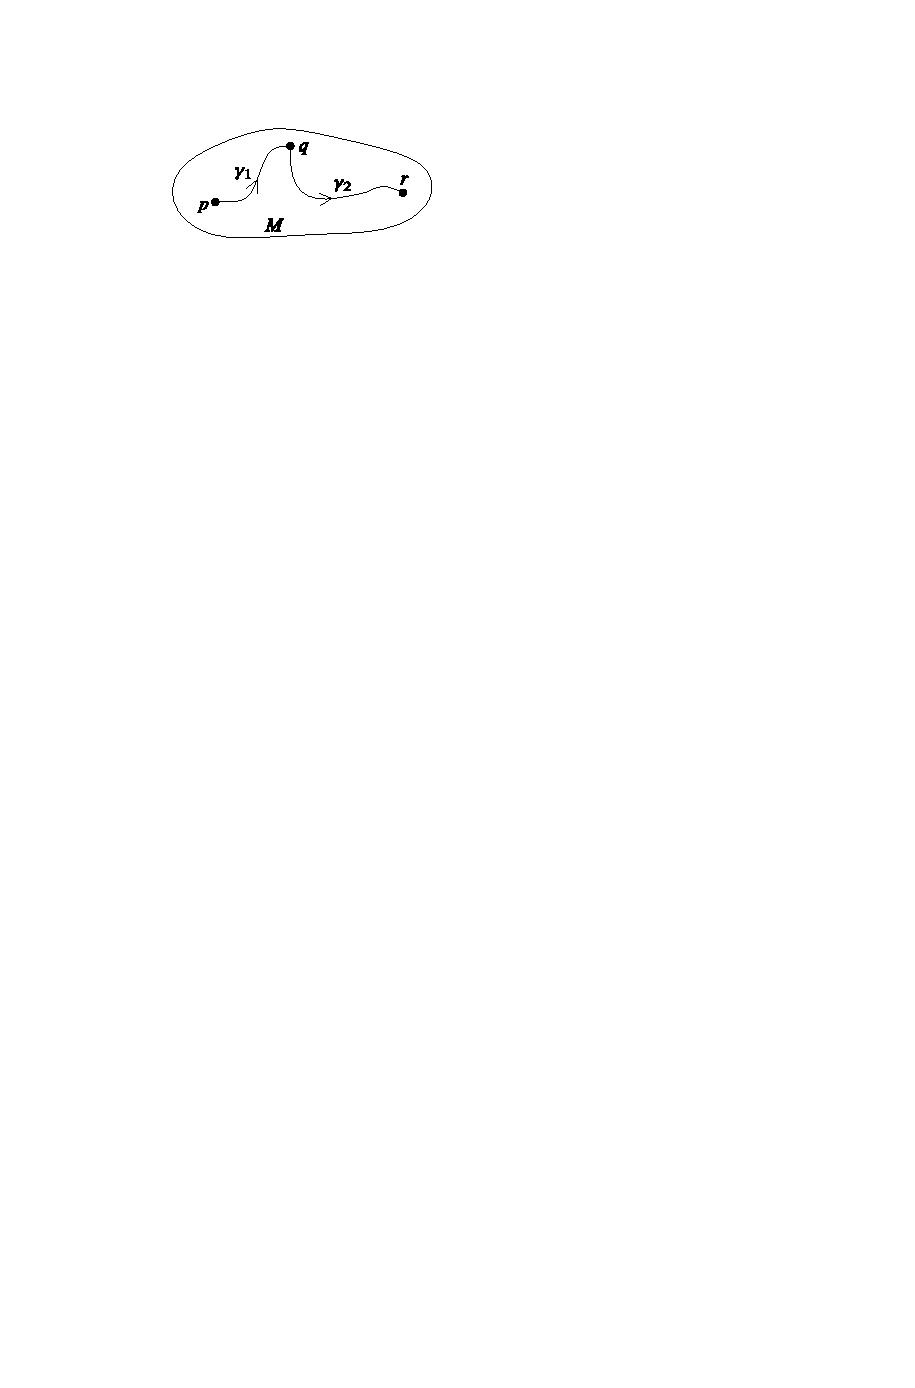
\includegraphics{pictures/Riemann-metric-1}
\caption{The triangle inequality.}
\end{minipage}
\hspace{20pt}
\begin{minipage}[b]{200pt}
\centering
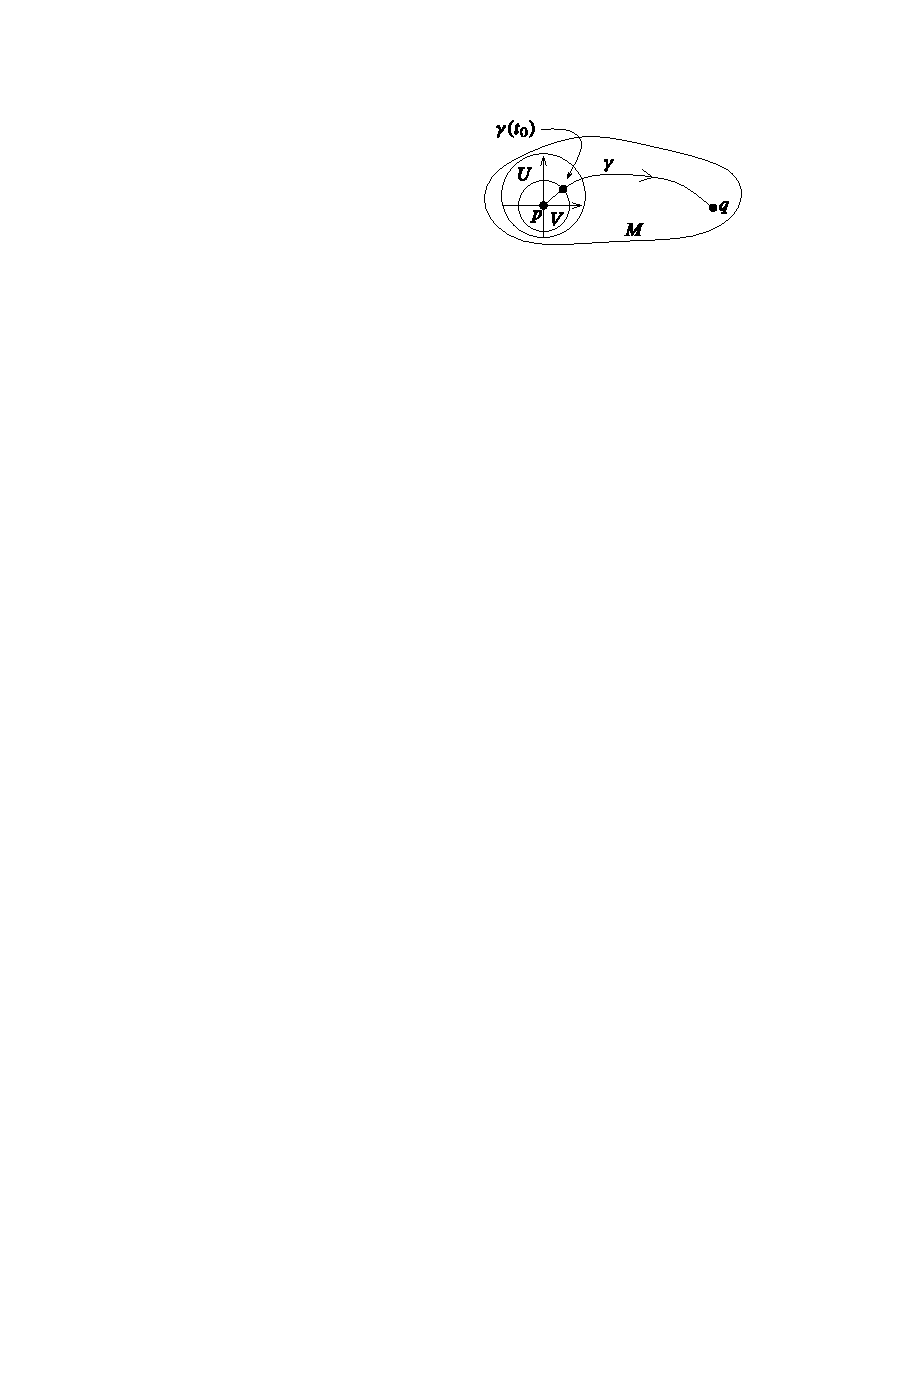
\includegraphics{pictures/Riemann-metric-2}
\caption{Positivity of $d_g$.}
\end{minipage}
\end{figure}
To complete the proof that $(M,d_g)$ is a metric space, we need only show that $d_g(p,q)>0$ if $p\neq q$. For this purpose, let $p,q\in M$ be distinct points, and let
$U$ be a smooth coordinate domain containing $p$ but not $q$. Use the coordinate map as usual to identify $U$ with an open subset in $\R^n$, and let $\widebar{g}$ denote the Euclidean metric in these coordinates. If $V$ is a regular coordinate ball of radius $\eps$ centered at $p$ such that $\widebar{V}\sub U$, Lemma~\ref{Riemann metric lem} shows that there are positive constants $c,C$ such that $(\ref{Riemann metric-1})$ is satisfied whenever $x\in\widebar{V}$ and $v\in T_xM$. Then for any piecewise smooth curve segment $\gamma$ lying entirely in $\widebar{V}$, it follows that
\[cL_{\widebar{g}}(\gamma)\leq L_g(\gamma)\leq CL_{\widebar{g}}(\gamma)\]
Suppose $\gamma:[a,b]\to M$ is a piecewise smooth curve segment from $p$ to $q$. Let $t_0$ be the infimum of all $t\in[a,b]$ such that $\gamma(t)\notin\widebar{V}$. It follows that $\gamma(t_0)\in\partial V$ by continuity, and $\gamma(t)\in\widebar{V}$ for $a\leq t\leq t_0$. Thus
\[L_g(\gamma)\geq L_g(\gamma|_{[a,t_0]})\geq cL_{\widebar{g}}(\gamma_{[a,t_0]})\geq cd_{\widebar{g}}(p,\gamma(t_0))=c\eps\]
Taking the infimum over all such $\gamma$, we conclude that $d_g(p,q)\geq c\eps>0$.\par
Finally, to show that the metric topology generated by $d_g$ is the same as the given manifold topology on $M$, we need to show that the open subsets in the manifold 
topology are open in the metric topology, and vice versa.\par
Suppose, first, that $U\sub M$ is open in the manifold topology. Let $p\in U$, and let $V$ be a regular coordinate ball of radius $\eps$ around $p$ such that 
$\widebar{V}\sub U$ as above. The argument in the previous paragraph shows that $d_g(p,q)\geq c\eps$ whenever $q\notin\widebar{V}$. The contrapositive of this 
statement is that $d_g(p,q)<c\eps$ implies $q\in\widebar{V}\sub U$, or in other words, the metric ball of radius $c\eps$ around $p$ is contained in $U$. This 
shows that $U$ is open in the metric topology.\par
Conversely, suppose that $W$ is open in the metric topology, and let $p\in W$. Let $V$ be a regular coordinate ball of radius $r$ around $p$, let $\widebar{g}$ 
be the Euclidean metric on $\widebar{V}$ determined by the given coordinates, and let $c,C$ be positive constants such that $(\ref{Riemann metric-1})$ is satisfied 
for $v\in T_qM,q\in\widebar{V}$. Let $\eps<r$ be a positive number small enough that the metric ball around $p$ of radius $C\eps$ is contained in $W$, and let 
$V_\eps$ be the set of points in $\widebar{V}$ whose Euclidean distance from $p$ is less than $\eps$. If $q\in V_\eps$, let $\gamma$ be the straight-line segment 
in coordinates from $p$ to $q$. Using Lemma~\ref{Riemann metric lem} as above, we conclude that
\[d_g(p,q)\leq L_g(\gamma)\leq CL_{\widebar{g}}(\gamma)<C\eps\]
This shows that $V_\eps$ is contained in the metric ball of radius $C\eps$ around $p$, and therefore in $W$. Since $V_\eps$ is a neighborhood of $p$ in the manifold 
topology, this shows that $W$ is open in the manifold topology as well.
\end{proof}
As a consequence of this theorem, all of the terminology of metric spaces 
can be carried over to connected Riemannian manifolds. Thus, a connected 
Riemannian manifold $(M,g)$ is said to be \textbf{complete}, and $g$ is 
said to be a \textbf{complete Riemannian metric}, if $(M,d_g)$ is a 
complete metric space (i.e., if every Cauchy sequence in $M$ converges 
to a point in $M$); and a subset $B\sub M$ is said to be \textbf{bounded} 
if there  exists a constant $K$ such that $d_g(x,y)\leq K$ for all 
$x,y\in B$; if this is the case, the \textbf{diameter} of $A$ is the smallest 
such constant:
\[\diam(A)=\sup\{d_g(p,q):p,q\in A\}\]
Since every compact metric space is bounded, every compact connected 
Riemannian manifold with or without boundary has finite diameter. 
(Note that the unit sphere with the Riemannian distance determined by 
the round metric has diameter $\pi$, not $2$, since the Riemannian distance 
between antipodal points is $\pi$).\par
Recall that a topological space is said to be \textbf{metrizable} if it 
admits a distance function whose metric topology is the same as the given 
topology.
\begin{corollary}
Every smooth manifold with or without boundary is metrizable.
\end{corollary}
\begin{proof}
First suppose $M$ is a smooth manifold without boundary, and choose any Riemannian metric $g$ on $M$. If $M$ is connected, Theorem~\ref{Riemann metric space} shows that $M$ is metrizable. More generally, let $\{M_i\}$ be the connected components of $M$, and choose a point $p_i\in M_i$ for each $i$. For $x\in M_i$ and $y\in M_j$, define $d_g(x,y)$ as in Theorem~\ref{Riemann metric space} when $i=j$, and otherwise
\[d_g(x,y)=d_g(x,p_i)+1+d_g(p_j,y)\]
It is straightforward to check that this is a distance function that induces the given topology on $M$. Finally, if $M$ has nonempty boundary, just embed $M$ into its double, and note that a subspace of a metrizable topological space is always metrizable.
\end{proof}
\subsection{Pseudo-Riemannian metrics}
From the point of view of geometry, Riemannian metrics are by far the most 
important structures that manifolds carry. However, there is a generalization 
of Riemannian metrics that has become especially important because of its 
application to physics.\par
Before defining this generalization, we begin with some linear-algebraic 
preliminaries. Suppose $V$ is a finite-dimensional vector space, and $q$ is 
a symmetric covariant $2$-tensor on $V$ (also called a symmetric bilinear 
form). Just as for an inner product, there is a linear map $\widehat{q}:V\to V^*$ 
defined by
\[\widehat{q}(v)(w)=q(v,w)\]
for $v,w\in V$. We say that $q$ is \textbf{nondegenerate} if $\widehat{q}$ is an isomorphism.
\begin{lemma}
Suppose $q$ is a symmetric covariant $2$-tensor on a finite-dimensional vector 
space $V$. The following are equivalent:
\begin{itemize}
\item[(a)] $q$ is nondegenerate.
\item[(b)] For every nonzero $v\in V$, there is some $w\in V$ such that $q(v,w)\neq 0$.
\item[(c)] If $q=q_{ij}\eps^i\eps^j$ in terms of some basis $(\eps^i)$ for $V^*$, 
then the matrix $(q_{ij})$ is invertible. 
\end{itemize}
\end{lemma}
\begin{proof}
By dimension consideration, $\widehat{q}$ is an isomorphism if and only if it is injective, so (a) 
is equivalent to (b). Now if $q(v,w)=0$, then in terms of matrix, we have $X^T(g_{ij})Y=0$ for some 
vector $X$ and every vector $Y$. This implies that $X^T(g_{ij})=0$, and thus $(g_{ij})X=0$ since $q$ 
is symmetric. This then implies that $(g_{ij})$ is not invertible, if $X\neq 0$. 
\end{proof}
We use the term \textbf{scalar product} to denote any nondegenerate 
symmetric bilinear form on a finite-dimensional vector space $V$, and 
reserve the term inner product for the special case of a positive definite 
scalar product. A \textbf{scalar product space} is a finite-dimensional 
vector space endowed with a scalar product. When convenient, we will often 
use a notation like $\langle\cdot\,\cdot\rangle$ to denote a scalar product. 
We say that vectors $v,w\in V$ are orthogonal if $\langle v,w\rangle=0$, 
just as in the case of an inner product. Given a vector $v\in V$, we define 
the \textbf{norm} of $v$ to be $|v|=|\langle v,v\rangle|^{1/2}$. Note that in the indefinite 
case, it is possible for a nonzero vector to be orthogonal to itself, and 
thus to have norm zero.\par
If $S\sub V$ is any linear subspace, the set of vectors in $V$ that are 
orthogonal to every vector in $S$ is a linear subspace denoted by $S^{\bot}$.
\begin{lemma}
Suppose $(V,q)$ is a finite-dimensional scalar product space, and $S\sub V$ 
is a linear subspace.
\begin{itemize}
\item[(a)] $\dim S+\dim S^{\bot}=\dim V$.
\item[(b)] $(S^\bot)^{\bot}=S$. 
\end{itemize}
\end{lemma}
\begin{proof}
Define a linear map $\varPhi:V\to S^*$ by $\varPhi(v)=\widehat{q}(v)|_S$. Note 
that $v\in\ker\varPhi$ if and only if $q(v,x)=0$ for all $x\in S$, so $\ker\varPhi=S^{\bot}$. 
If $\varphi\in S^*$ is arbitrary, there is a covector $\widetilde{\varphi}\in V^*$ 
whose restriction to $S$ is equal to $\varphi$. (For example, such a covector 
is easily constructed after choosing a basis for $S$ and extending it to a basis 
for $V$.) Since $\widehat{q}$ is an isomorphism, there exists $v\in V$ such 
that $\widehat{q}(v)=\widetilde{\varphi}$. It follows that $\varPhi(v)=\varphi$, 
and therefore $\varPhi$ is surjective. By the rank–nullity theorem, the dimension 
of $S^{\bot}=\ker\varPhi$ is equal to $\dim V-\dim S^*=\dim V-\dim S$. This 
proves (a).\par
To prove (b), note that every $v\in S$ is orthogonal to every element of $S$ by 
definition, so $S\sub (S^{\bot})^{\bot}$. Because these finite-dimensional vector 
spaces have the same dimension by part (a), they are equal.
\end{proof}
An ordered $k$-tuple $(v_1,\dots,v_k)$ of elements of $V$ is said to be \textbf{orthonormal} 
if $|v_i|=1$ for each $i$ and $\langle v_i,v_j\rangle=0$ for $i\neq j$, or 
equivalently, if $\langle v_i,v_j\rangle=\delta_{ij}$ for each $i$ and $j$. We wish 
to prove that every scalar product space has an orthonormal basis. Note that 
the usual Gram–Schmidt algorithm does not always work in this situation, because 
the vectors that appear in the denominators might have vanishing norms. In 
order to get around this problem, we introduce the following definitions.\par
If $(V,q)$ is a finite-dimensional scalar product space, a subspace $S\sub V$ 
is said to be nondegenerate if the restriction of $q$ to $S\times S$ is nondegenerate. 
An ordered $k$-tuple of vectors $(v_1,\dots,v_k)$ in $V$ is said to be nondegenerate 
if for each $j=1,\dots,k$ the vectors $(v_1,\dots,v_j)$ span a nondegenerate 
$j$-dimensional subspace of $V$. For example, every orthonormal basis is nondegenerate.
\begin{lemma}\label{scalar prod nondegenerate}
Suppose $(V,q)$ is a finite-dimensional scalar product space, and $S\sub V$ is 
a linear subspace. The following are equivalent:
\begin{itemize}
\item[(a)] $S$ is nondegenerate.
\item[(b)] $S^{\bot}$ is nondegenerate.
\item[(c)] $S\cap S^{\bot}=\{0\}$.
\item[(d)] $V=S\oplus S^{\bot}$.   
\end{itemize}
\end{lemma}
\begin{proof}
Note that $q|_S$ is nondegenerate if and only if the set
\[\{x\in S:q(x,y)=0\forall y\in S\}=S\cap S^{\bot}\]
is $\{0\}$. Now since $(S^{\bot})^{\bot}=S$, we have the equivalences (a), (b) and (c). 
Now, since $\dim S+\dim S^{\bot}=\dim V$, they are easily seen to be equivalent to (d).
\end{proof}
\begin{lemma}[\textbf{Completion of Nondegenerate Bases}]\label{scalar prod complete nondegenerate base}
Suppose $(V,q)$ is an $n$-dimensional scalar product space, and $(v_1,\dots,v_k)$ 
is a nondegenerate $k$-tuple in $V$ with $0\leq k<n$. Then there exist vectors 
$v_{k+1},\dots,v_n\in V$ such that $(v_1,\dots,v_n)$ is a nondegenerate basis 
for $V$.
\end{lemma}
\begin{proof}
Let $S=\mathrm{span}(v_1,\dots,v_k)\sub V$. Because $k<n$, $S^{\bot}$ is a nontrivial 
subspace of $V$, and Lemma~\ref{scalar prod nondegenerate} shows that 
$S^{\bot}$ is nondegenerate and $V=S\oplus S^{\bot}$. By the nondegeneracy 
of $S^{\bot}$, there must be a vector in $S^{\bot}$ with nonzero length, 
because otherwise the polarization identity would imply that all inner 
products of pairs of elements of $S$ would be zero. If $v_{k+1}\in S^{\bot}$ 
is any vector with nonzero length, then $(v_1,\dots,v_{k+1})$ is easily 
seen to be a nondegenerate $(k+1)$-tuple. Repeating this argument for 
$v_{k+2},\dots,v_n$ completes the proof.
\end{proof}
\begin{proposition}[\textbf{Gram–Schmidt Algorithm for Scalar Products}]
Suppose $(V,q)$ is an $n$-dimensional scalar product space. If $(v_i)$ is a 
nondegenerate basis for $V$, then there is an orthonormal basis $(b_i)$ with 
the property that $\mathrm{span}(b_1,\dots,b_k)=\mathrm{span}(v_1,\dots,v_k)$ 
for each $k=1,\dots,n$.
\end{proposition}
\begin{proof}
As in the positive definite case, the basis $(b_i)$ is constructed recursively, 
starting with $b_1=v_1/|v_1|$ and noting that the assumption that $v_1$ spans 
a nondegenerate subspace ensures that $|v_1|\neq 0$. At the inductive step, 
assuming we have constructed $(b_1,\dots,b_k)$, we first set
\[z=v_{k+1}-\sum_{i=1}^{k}\frac{\langle v_{k+1},b_i\rangle}{\langle b_i,b_i\rangle}b_i.\]
Each denominator $\langle b_i,b_i\rangle$ is equal to $\pm 1$, so this defines 
$z$ as a nonzero element of $V$ orthogonal to $b_1,\dots,b_k$, and with the 
property that $\mathrm{span}(b_1,\dots,b_k,z)=\mathrm{span}(v_1,\dots,v_{k+1})$. 
If $\langle z,z\rangle=0$, then $z$ is orthogonal to $\mathrm{span}(v_1,\dots,v_{k+1})$, 
contradicting the nondegeneracy assumption. Thus we can complete the inductive step 
by putting $b_{k+1}=z/|z|$.
\end{proof}
\begin{corollary}
Suppose $(v,q)$ is an $n$-dimensional scalar product space. There is a basis 
$(\beta^i)$ for $V^*$ with respect to which $q$ has the expression
\begin{align}\label{scalar prod canonical form}
q=(\beta^1)^2+\cdots+(\beta^r)^2-(\beta^{r+1})^2-\cdots-(\beta^{r+s})^2,
\end{align}
for some nonnegative integers $r,s$ with $r+s=n$.
\end{corollary}
\begin{proof}
Let $(b_i)$ be an orthonormal basis for $V$, and let $(\beta^i)$ be the dual 
basis for $V^*$. A computation shows that $q$ has a basis expression of the 
form $(\ref{scalar prod canonical form})$, but perhaps with the positive and 
negative terms in a different order. Reordering the basis so that the positive 
terms come first, we obtain $(\ref{scalar prod canonical form})$.
\end{proof}
It turns out that the numbers $r$ and $s$ in $(\ref{scalar prod canonical form})$ are independent of the choice of
basis. The integer $s$ in the expression (the number of negative terms) is called 
the \textbf{index} of $q$, and the ordered pair $(r,s)$ is called the \textbf{signature} of $q$.\par
Now suppose $M$ is a smooth manifold. A \textbf{pseudo-Riemannian metric} on $M$ (called 
by some authors a semi-Riemannian metric) is a smooth symmetric $2$-tensor field 
$g$ that is nondegenerate at each point of $M$, and with the same signature 
everywhere. Every Riemannian metric is also a pseudo-Riemannian metric.
\begin{proposition}[\textbf{Orthonormal Frames for Pseudo-Riemannian Manifolds}]\label{pseudo Riemann orthonormal frame}
Let $(M,g)$ be a pseudo-Riemannian manifold. For each $p\in M$, there exists 
a smooth orthonormal frame on a neighborhood of $p$ in $M$.
\end{proposition}
\begin{example}
Suppose $(M_1,g_1)$ and $(M_2,g_2)$ are pseudo-Riemannian manifolds of signatures $(r_1,s_1)$ 
and $(r_2,s_2)$, respectively. Then $(M_1\times M_2,g_1\oplus g_2)$ is a 
pseudo-Riemannian manifold of signature $(r_1+r_2,s_1+s_2)$.
\end{example}
For nonnegative integers $r$ and $s$, we define the \textbf{pseudo-Euclidean space of signature \bm{$(r,s)$}}, 
denoted by $\R^{r,s}$, to be the manifold $\R^{r+s}$, with standard coordinates 
denoted by $(\xi^1,\dots,\xi^r,\tau^1,\dots,\tau^s)$, and with the pseudo-Riemannian 
metric $\widebar{q}^{(r,s)}$ defined by
\[\widebar{q}^{(r,s)}=(d\xi^1)^2+\cdots+(d\xi^r)^2-(d\tau^1)^2-\cdots-(d\tau^s)^2.\]
By far the most important pseudo-Riemannian metrics (other than the Riemannian ones) 
are the \textbf{Lorentz metrics}, which are pseudo-Riemannian metrics of 
index $1$, and thus signature $(r,1)$.\par 
The pseudo-Euclidean metric $\widebar{q}^{(r,1)}$ is a \textbf{Lorentz metric} 
called the \textbf{Minkowski metric}, and the Lorentz manifold $\R^{r,1}$ is 
called $(r+1)$-dimensional Minkowski space. If we denote standard coordinates 
on $\R^{r+1}$ by $(\xi^1,\dots,\xi^r,\tau)$ then the Minkowski metric is given by
\[\widebar{q}^{(r,1)}=(d\xi^1)^2+\cdots+(d\xi^r)^2-(d\tau^1)^2.\]

Many, but not all, results from the theory of Riemannian metrics apply 
equally well to pseudo-Riemannian metrics. We will attempt to point out 
which results carry over directly to pseudo-Riemannian metrics, which ones 
can be adapted with minor modifications, and which ones do not carry over 
at all. As a rule of thumb, proofs that depend only on the nondegeneracy of 
the metric tensor, such as properties of the musical isomorphisms and 
existence and uniqueness of geodesics, work fine in the pseudo-Riemannian 
setting, while proofs that use positivity in an essential way, such as 
those involving lengths of curves, do not.\par
One notable result that does not carry over to the pseudo-Riemannian case 
is Proposition~~\ref{Riemann metric space}, about the existence of metrics. 
For example, the following result characterizes those manifolds that admit 
Lorentz metrics.
\begin{theorem}\label{Riemann Lorenta metric}
A smooth manifold $M$ admits a Lorentz metric if and only if it admits a 
rank-$1$ tangent distribution (i.e., a rank-$1$ subbundle of $TM$).
\end{theorem}
\begin{proof}
For sufficiency, assume that $D\sub TM$ is a $1$-dimensional distribution, 
and choose any Riemannian metric $g$ on $M$. Then, by Lemma~\ref{vector subbundle crit}, 
locally it is possible to choose a $g$-orthonormal frame $(E_i)$ and dual 
coframe $(\eps^i)$ such that $E_1$ spans $D$. Then the Lorentz metric 
$-(\eps^1)^2+(\eps^2)^2+\cdots+(\eps^n)^2$ is independent of the choice of 
frame.
\end{proof}
\subsubsection{Pseudo-Riemannian submanifolds}
The theory of submanifolds is only slightly more complicated in the 
pseudo-Riemannian case. If $(\widetilde{M},\widetilde{g})$ is a 
pseudo-Riemannian manifold, a smooth submanifold $\iota:M\hookrightarrow\widetilde{M}$ 
is called a \textbf{pseudo-Riemannian submanifold} of $\widetilde{M}$ if $\iota^*\widetilde{g}$ 
is nondegenerate with constant signature. If this is the case, we always 
consider $M$ to be endowed with the induced pseudo-Riemannian metric $\iota^*\widetilde{g}$. 
In the special case in which $\iota^*\widetilde{g}$ is positive definite, 
$M$ is called a \textbf{Riemannian submanifold}.\par
The nondegeneracy hypothesis is not automatically satisfied: for example, 
if $M\sub\R^{1,1}$ is the submanifold $\{(\xi,\tau):\tau=\xi\}$ and $\iota:M\to\R^{1,1}$ 
is inclusion, then the pullback tensor $\iota^*\widetilde{g}$ is identically 
zero on $M$.\par
For hypersurfaces (submanifolds of codimension $1$), the nondegeneracy 
condition is easy to check. If $M\sub\widetilde{M}$ is a smooth 
submanifold and $p\in M$, then a vector $v\in T_p\widetilde{M}$ is said to 
be \textbf{normal to $\bm{M}$} if $\langle v,x\rangle=0$ for all $x\in T_pM$, 
just as in the Riemannian case. The space of all normal vectors at $p$ is 
a subspace of $T_p\widetilde{M}$ denoted by $N_pM$.
\begin{proposition}\label{pseudo Riemann submani}
Suppose $(\widetilde{M},\widetilde{g})$ is a pseudo-Riemannian manifold of 
signature $(r,s)$. Let $M$ be a smooth hypersurface in $\widetilde{M}$, and 
let $\iota:M\to\widetilde{M}$ be the inclusion map. Then the pullback 
tensor field $\iota^*\widetilde{g}$ is nondegenerate if and only if $\widetilde{g}(v,v)\neq 0$ 
for every $p\in M$ and every nonzero normal vector $v\in N_pM$. If $\widetilde{g}(v,v)>0$ 
for every nonzero normal vector to $M$, then $M$ is a pseudo-Riemannian 
submanifold of signature $(r-1,s)$; and if $\widetilde{g}(v,v)<0$ for every 
such vector, then $M$ is a pseudo-Riemannian submanifold of signature $(r,s-1)$.
\end{proposition}
\begin{proof}
Given $p\in M$, Lemma~\ref{scalar prod nondegenerate} shows that $T_pM$ is 
a nondegenerate subspace of $T_p\widetilde{M}$ if and only if the one-dimensional 
subspace $(T_pM)^{\bot}=N_pM$ is nondegenerate, which is the case if and only 
if every nonzero $v\in N_pM$ satisfies $\widetilde{g}(v,v)\neq 0$.\par
Now suppose $\widetilde{g}(v,v)>0$ for every nonzero normal vector $v$. Let 
$p\in M$ be arbitrary, and let $v$ be a nonzero element of $N_pM$. Writing 
$n=\dim \widetilde{M}$, we can complete $v$ to a nondegenerate basis $v,w_2,\dots,w_n$ 
for $T_pM$ by Lemma~\ref{scalar prod complete nondegenerate base}, and then 
use the Gram–Schmidt algorithm to find an orthonormal basis $b_1,\dots,b_n$ for $T_p\widetilde{M}$ 
such that $\mathrm{span}(b_1)=N_pM$. It follows that $\mathrm{span}(b_2,\dots,b_n)=T_pM$. 
If $(\beta^j)$ is the dual basis to $(b_i)$, then $\widetilde{g}_p$ has a 
basis representation of the form $(\beta^1)^2\pm(\beta^2)^2\pm\cdots\pm(\beta^n)^2$, 
with a total of $r$ positive terms and $s$ negative ones, and with a positive 
sign on the first term $(\beta^1)^2$. Therefore, $\iota^*\widetilde{g}_p=\pm(\beta^2)^2\pm\cdots\pm(\beta^n)^2$ 
has signature $(r-1,s)$. The argument for the case $\widetilde{g}(v,v)<0$ is similar.
\end{proof}
If $(M,g)$ is a pseudo-Riemannian manifold and $f\in C^{\infty}(M)$, then 
the \textbf{gradient} of $f$ is defined as the smooth vector field $\grad f=(df)^{\sharp}$ 
just as in the Riemannian case.
\begin{proposition}
Suppose $(\widetilde{M},\widetilde{g})$ is a pseudo-Riemannian manifold of 
signature $(r,s)$, $f\in C^{\infty}(M)$, and $M=f^{-1}(c)$ for some $c\in\R$. 
If $\langle\grad f,\grad f\rangle>0$ everywhere on $M$, then $M$ is an 
embedded pseudo-Riemannian submanifold of $M$ of signature $(r-1,s)$ and if 
$\langle\grad f,\grad f\rangle<0$  everywhere on $M$, then $M$ is an embedded 
pseudo-Riemannian submanifold of $\widetilde{M}$ of signature $(r,s-1)$. In 
either case,$\grad f$ is everywhere normal to $M$.
\end{proposition}
\begin{proof}
By Proposition~\ref{regular value level set} and Proposition~\ref{tangent space level set} 
we know that $M$ is an embedded submanifold whose tangent space is every where tangent to 
$\grad f$. Now the result follows from Proposition~\ref{pseudo Riemann submani}.
\end{proof}
\begin{proposition}[\textbf{Pseudo-Riemannian Adapted Orthonormal Frames}]
Suppose $(\widetilde{M},\widetilde{g})$ is a pseudo-Riemannian manifold, 
and $M\sub\widetilde{M}$ is an embedded pseudo-Riemannian or Riemannian 
submanifold. For each $p\in M$, there exists a smooth orthonormal frame on 
a neighborhood of $p$ in $\widetilde{M}$ that is adapted to $M$.
\end{proposition}
\begin{proof}
Write $m=\dim\widetilde{M}$ and $n=\dim M$, and let $p\in M$ be arbitrary. 
Proposition~\ref{pseudo Riemann orthonormal frame} shows that there is a 
smooth orthonormal frame $(E_1,\dots,E_n)$ for $M$ on some neighborhood of 
$p$ in $M$. Then by Lemma~\ref{scalar prod complete nondegenerate base}, we can find vectors $v_{n+1},\dots,v_m$ 
such that 
\[(E_1|_p,\dots,E_n|_p,v_{n+1},\dots,v_m)\]
is a nondegenerate basis for $T_p\widetilde{M}$. Now extend $v_{n+1},\dots,v_m$ arbitrarily to 
smooth vector fields $V_{m+1},\dots,V_m$ on a neighborhood of $p$ in $\widetilde{M}$. 
By continuity, the ordered $m$-tuple 
\[(E_1,\dots,E_n,V_{n+1},\dots,V_m)\] 
will be a nondegenerate frame for $\widetilde{M}$ in some (possibly smaller) 
neighborhood of $p$. Applying the Gram–Schmidt algorithm to this local 
frame yields a smooth local orthonormal frame $(E_1,\dots,E_m)$ for $\widetilde{M}$ 
with the property that $(E_1,\dots,E_n)$ restricts to a local orthonormal 
frame for $M$.
\end{proof}
The next corollary is proved in the same way as Proposition~\ref{Riemann normal bundle}
\begin{corollary}[\textbf{Normal Bundle to a Pseudo-Riemannian Submanifold}]
Suppose $(\widetilde{M},\widetilde{g})$ is a pseudo-Riemannian manifold, 
and $M\sub\widetilde{M}$ is an embedded pseudo-Riemannian or Riemannian 
submanifold. The set of vectors normal to $M$ is a smooth vector subbundle 
of $T\widetilde{M}|_M$, called the normal bundle to $M$.
\end{corollary}
\subsection{Exercise}
\begin{exercise}\label{vector bundle convex subset}
Suppose that $E$ is a smooth vector bundle over a smooth manifold $M$ with or without boundary, and $V\sub E$ is an open subset with the property that for each $p\in M$, the intersection of $V$ with the fiber $E_p$ is convex and nonempty. By a section of $V$, we mean a section of $E$ whose image lies in $V$.
\begin{itemize}
\item[(a)] Show that there exists a smooth global section of $V$.
\item[(b)] Suppose $\sigma:A\to V$ is a smooth section of $V$ defined on a closed subset $A\sub M$. $($This means that $\sigma$ extends to a smooth section of $V$ in a
neighborhood of each point of $A$.$)$ Show that there exists a smooth global section $\widetilde{\sigma}$ of $V$ whose restriction to $A$ is equal to $\sigma$. Show that if $V$ contains the image of the zero section of $E$, then $\widetilde{\sigma}$ can be chosen to be supported in any predetermined neighborhood of $A$.
\end{itemize}
\end{exercise}
\begin{proof}
For $p\in M$, choose a neighborhood $U$ contains $p$, with a local 
trivialization $\varPhi:\pi^{-1}(U)\to U\times\R^k$. Let $v\in\R^k$ be a 
vector such that $(p,v)\in\varPhi\big(V\cap\pi^{-1}(U)\big)$. Since 
$V\cap\pi^{-1}(U)$ is open, by appropriately shrinking $U$, we can find 
an open subset $W\sub\R^k$ such that 
\[(p,v)\in U\times W\sub\varPhi\big(V\cap\pi^{-1}(U)\big).\]
In particular, $(q,v)\in\varPhi\big(V\cap\pi^{-1}(U)\big)$ for all $q\in U$, thus we can define $\sigma_p:U\to E$ by
\[\sigma_p(q)=\varPhi^{-1}(q,v)\for q\in U.\]
It follows that $\sigma_p$ is a local section of $V$. Now the neighborhoods $\{U_p\}$ gives an open cover of $M$, by taking a partition of unity $\{\psi_p\}$ for the open cover $\{\psi_p\}$, we define
\[\eta=\sum_{p\in M}\psi_p\sigma_p.\]
Then at each point $p_0$, since $V\cap E_{p_0}$ is convex, we find $\eta(p_0)\in V$.\par
The second statement is the same as Lemma~\ref{ext lem smooth func}.
\end{proof}
\begin{exercise}
Prove that every Riemannian $1$-manifold is flat.
\end{exercise}
\begin{proof}
Let $M$ be a Riemannian $1$-manifold, then each point of $M$ admits a commuting orthonormal frame. Thus by Proposition~\ref{Riemann flat iff} $M$ is flat.
\end{proof}
\begin{exercise}\label{isometry is linear}
Suppose $V$ and $W$ are finitely-dimensional real inner product spaces of the same dimension, and $F:V\to W$ is any map (not assumed to be linear or even continuous) that 
preserves the origin and all distances: $F(0)=0$ and $|F(x)-F(y)|=|x-y|$ for all $x,y\in V$. Prove that $F$ is a linear isometry.
\end{exercise}
\begin{proof}[First proof]
First, inserting $y=0$ in the second condition gives $|F(x)|=|x|$. Now let $t\in[0,1]$ and denote $r=|x-y|$. Then 
\[\{tx+(1-t)y\}=\widebar{B}(x,tr)\cap\widebar{B}(y,(1-t)r).\]
Now since $F$ is injective, $F(tx+(1-t)y)$ is the unique element of 
\[F(\widebar{B}(x,tr)\cap\widebar{B}(y,(1-t)r))=F(\widebar{B}(x,tr))\cap F(\widebar{B}(y,(1-t)r))=\widebar{B}(F(x),tr)\cap\widebar{B}(F(y),(1-t)r),\]
which is $tF(x)+(1-t)F(y)$. This then implies $F(x)$ is linear since $F(0)=0$.
\end{proof}
\begin{proof}[Second proof]
We have $|F(x)|=x$ for all $x\in V$. Now expand the equation $|F(x)-F(y)|^2=|x-y|^2$, we get
\[|F(x)|^2+|F(y)|^2-2(F(x),F(y))=|x|^2+|y|^2-2(x,y).\]
Therefore $F$ preserves the inner products.\par
Now let $x,y\in V$, we want to prove $F(x+y)=F(x)+F(y)$ and $F(\lambda x)=\lambda x$ for $\lambda\in\R$. We note that for all $v\in V$,
\begin{align*}
(F(x+y),F(v))=((x+y),v)=(x,v)+(y,v)=(F(x)+F(y),F(v)).
\end{align*}
Take $v$ to be a orthonormal basis for $V$, this then implies $F(x+y)=F(x)+F(y)$. Similarly we can prove $F(\lambda x)=\lambda F(x)$, therefore $F$ is linear.
\end{proof}
\begin{exercise}\label{Euclidean shortest path}
Show that the shortest path between two points in Euclidean space is a straight line segment. More precisely, for $x,y\in\R^n$, let $\gamma:[0,1]\to\R^n$ be the 
curve segment $\gamma(t)=x+t(y-x)$, and show that any other piecewise smooth curve segment $\widetilde{\gamma}$ from $x$ to $y$ satisfies 
$L_{\widebar{g}}(\widetilde{\gamma})\geq L_{\widebar{g}}(\gamma)$.
\end{exercise}
\begin{proof}
Let $\gamma:[a,b]\to\R^n$ be a piecewise smooth curve segment such that $\gamma(a)=x$ and $\gamma(b)=y$. 
For any constant vector $v$ with $|v|=1$, by Cauchy-Schwarz inequality we have
\[(y-x)\cdot v=\big(\gamma(t)\cdot v\big)\Big|_{t=a}^{t=b}=\int_{a}^{b}\gamma'(t)\cdot v\,dt\leq\int_{a}^{b}|\gamma'(t)||v|dt=\int_{a}^{b}|\gamma'(t)|dt.\]
Set $v=(y-x)/|y-x|$, then
\[|y-x|\leq\int_{a}^{b}|\gamma'(t)|dt.\]
Now if the equality holds if and only if $\gamma'(t)=a(y-x)$ for some constant $a\in\R$. 
Hence if and only if $\gamma(t)=a(y-x)t+b$ with $a,b\in\R$.
\end{proof}
\begin{exercise}\label{Euclidean isometry group}
Consider $\R^n$ as a Riemannian manifold with the Euclidean metric $\widebar{g}$.
\begin{itemize}
\item[(a)] Suppose $U,V\sub\R^n$ are connected open sets, $\varphi,\psi:U\to V$ are Riemannian isometries, and for some $p\in U$ they satisfy $\varphi(p)=\psi(p)$ and $d\varphi_p=d\psi_p$. Show that $\varphi=\psi$.
\item[(b)] Show that the set of maps from $\R^n$ to itself given by the action of $E(n)$ on $\R^n$ described in Example~\ref{Euclidean group} is the full group of Riemannian isometries of $(\R^n,\widebar{g})$.
\end{itemize}
\end{exercise}
\begin{proof}
Let $x\in\R^n$, and let $\gamma$ be a smooth curve in $\R^n$ from $\varphi(p)$ to $\varphi(x)$, 
then by Proposition~\ref{Riemann isometry length},
\[L_{\widebar{g}}(\gamma)=L_{\widebar{g}}(\varphi^{-1}\circ\gamma)\geq L_{\widebar{g}}(\sigma)=L_{\widebar{g}}(\varphi\circ\sigma),\]
where $\sigma:[0,1]\to\R^n$ is the straight line from $p$ to $x$ and we use the result of Exercise~\ref{Euclidean shortest path}. 
This implies that $\varphi\circ\sigma$ is the straight line from $\varphi(p)$ to $\varphi(x)$. 
Since the length of $\varphi\circ\sigma$ is fixed, $\varphi(x)$ is uniquely determined by its 
direction, that is, $(\varphi\circ\sigma)'(0)$. Since $d\varphi_p=d\psi_p$ we then conclude 
$\varphi=\psi$.\par
Let $\varphi$ be any Riemannian isometry of $(\R^n,\widebar{g})$. Since $d\varphi_0$ preserves 
the Euclidean dot product, it corresponds to a matrix $C\in\O(n)$. Let $(\varphi(0),C)\in E(n)$, then $\varphi$ is represented by $(C,\varphi(0))$, in the sense that
\[\varphi(x)=(\varphi(0),C)\cdot x=\varphi(0)+Cx.\]
This gives the claim.
\end{proof}
\begin{exercise}
Let $(M,g)$ be a Riemannian manifold. A smooth vector field $V$ on $M$ is called a \textbf{Killing vector field} for $g$ if the flow of $V$ acts by isometries of $g$.
\begin{itemize}
\item[(a)] Show that the set of all Killing vector fields on $M$ constitutes a Lie subalgebra of $\X(M)$.
\item[(b)] Show that a smooth vector field $V$ on $M$ is a Killing vector field if and only if it satisfies the following equation in each smooth local coordinate chart:
\[V^k\frac{\partial g_{ij}}{\partial x^k}+g_{jk}\frac{\partial V^k}{\partial x^i}+g_{ik}\frac{\partial V^k}{\partial x^j}=0\quad\text{for all }i,j.\]
\end{itemize}
\end{exercise}
\begin{proof}
By definition, $V$ is a killing field if and only if $g$ is invairant under $\theta$. Thus by Theorem~\ref{tensor filed invariant flow iff}, this is equivalent to $\mathfrak{L}_Vg=0$. Now by Exercise~\ref{tensor field Lie derivative bracket},
\[\mathfrak{L}_{[V,W]}g=\mathfrak{L}_V\mathfrak{L}_Wg-\mathfrak{L}_W\mathfrak{L}_Vg.\]
Thus part (a) follows.\par
For part (b), write $V=V^k\partial/\partial x^k$, we compute using Corollary~\ref{Lie derivative tensor}:
\begin{align*}
(\mathfrak{L}_Vg)\Big(\frac{\partial}{\partial x^i},\frac{\partial}{\partial x^j}\Big)&=V(g_{ij})-g\Big([V,\frac{\partial}{\partial x^i}],\frac{\partial}{\partial x^j}\Big)-g\Big(\frac{\partial}{\partial x^i},[V,\frac{\partial}{\partial x^j}]\Big)\\
&=V^k\frac{\partial g_{ij}}{\partial x^k}+g\Big(\frac{\partial V^k}{\partial x^i}\frac{\partial}{\partial x^k},\frac{\partial}{\partial x^j}\Big)+g\Big(\frac{\partial}{\partial x^i},\frac{\partial V^k}{\partial x^j}\frac{\partial}{\partial x^k}\Big)\\
&=V^k\frac{\partial g_{ij}}{\partial x^k}+g_{jk}\frac{\partial V^k}{\partial x^i}+g_{ik}\frac{\partial V^k}{\partial x^j}.
\end{align*}
\end{proof}
\begin{exercise}
Let $K\sub\X(\R^n)$ denote the Lie algebra of Killing vector fields with respect to the Euclidean metric, and let $K_0\sub K$ denote the
subspace consisting of fields that vanish at the origin.
\begin{itemize}
\item[(a)] Show that the map
\[V\mapsto\Big(\frac{\partial V^k}{\partial x^j}(0)\Big)\]
is an injective linear map from $K_0$ to $\o(n)$.
\item[(b)] Show that the following vector fields form a basis for $K$:
\[\frac{\partial}{\partial x^i},\quad 1\leq i\leq n;\quad\quad x^i\frac{\partial}{\partial x^j}-x^j\frac{\partial}{\partial x^i},\quad 1\leq i<j\leq n.\]
\end{itemize}
\end{exercise}
\begin{proof}
If $g=\delta_{ij}dx^idx^j$, then the equation becomes
\[\frac{\partial V^j}{\partial x^i}+\frac{\partial V^i}{\partial x^j}=0\]
thus the image of the map is in $\o(n)$.
\end{proof}
\begin{exercise}
Suppose $g=f(t)dt^2$ is a Riemannian metric on $\R$. Show that $g$ is complete if and only if both of the following improper integrals diverge:
\[\int_{0}^{+\infty}\sqrt{f(t)}dt,\quad\int_{-\infty}^{0}\sqrt{f(t)}dt.\]
\end{exercise}
\begin{exercise}\label{Riemann grad prop}
Let $(M,g)$ be a Riemannian manifold, let $f\in C^\infty(M)$, and let $p\in M$ be a regular point of $f$.
\begin{itemize}
\item[(a)] Show that among all unit vectors $v\in T_pM$, the directional derivative
$vf$ is greatest when $v$ points in the same direction as $\grad f|_p$, and the length of $\grad f|_p$ is equal to the value of the directional derivative in that direction.
\item[(b)] Show that $\grad f|_p$ is normal to the level set of $f$ through $p$.
\item[(c)] Let $X\in\X(M)$ be a nowhere-vanishing vector field. Prove that $X=\grad f$ if and only if $Xf\equiv|X|_g^2$ and $X$ is orthogonal to the level sets of $f$ 
at all regular points of $f$. 
\end{itemize}
\end{exercise}
\begin{proof}
By $(\ref{Riemann grad def})$ we have
\[\langle\grad f|_p,v\rangle_g=df_p(v)=vf.\]
Then by Cauchy-Schwarz inequality, we have
\[vf\leq |v|_g\cdot\big|\grad f|_p\big|_g,\]
with the quality holds if and only if $v$ is paralle to $\grad f|_p$.\par
Let $S=f^{-1}(f(p))$ be the level set of $f$ through $p$, then by Proposition~\ref{tangent space level set} we have
\[T_pS=\ker df_p=\ker(\widehat{g}(\grad f)_p)=\ker\big(\langle\grad f|_p,\cdot\rangle_g\big).\]
Thus $\grad f|_p$ is normal to $T_pS$.\par
For (c), one direction is clear. Conversely, assume that $X\in\X(M)$ satisfies the conditions. Let $S$ be a level set of $f$ and $p\in S$, then $\dim(T_pS)^{\bot}=1$ 
for $p\in S$. Since $X$ and $\grad f$ are both contained in it, is follows that $X_p=\lambda\grad f|_p$ for some $\lambda\in\R$. From the condition we have
\[\lambda\langle X_p,X_p\rangle\langle\grad f|_p,X_p\rangle=Xf|_p=\langle X_p,X_p\rangle=\lambda^2\langle X_p,X_p\rangle.\]
Therefore $\lambda=1$ since $X_p\neq 0$. Since $X$ is non-vanishing, it follows that $X=\grad f$.
\end{proof}
\begin{exercise}\label{Morse exercise}
Let $M$ be a compact smooth $n$-manifold, and suppose $f$ is a smooth real-valued function on $M$ that has only finitely many critical points $\{p_1,\dots,p_k\}$, with 
corresponding critical values $c_1,\dots,c_k$ labeled so that $c_1\leq \cdots\leq c_k$. For any $a<b\in\R$, define
\[M_a=f^{-1}(a),\quad M_{(a,b)}=f^{-1}(a,b),\quad M_{[a,b]}=f^{-1}([a,b]).\]
If $a$ and $b$ are regular values, note that $M_a$ and $M_b$ are embedded hypersurfaces in $M$, $M_{(a,b)}$ is an open submanifold, and $M_{[a,b]}$ is a regular domain by Proposition~\ref{regular domain}.
\begin{itemize}
\item[(a)] Choose a Riemannian metric $g$ on $M$, let $X$ be the vector field $X=\grad f/|\grad f|_g^2$ on $M\setminus\{p_1,\dots,p_k\}$, and let $\theta$ denote the 
flow of $X$. Show that $f(\theta_t(p))=f(p)+t$ whenever $\theta_t$ is defined.
\item[(b)] Let $[a,b]\times\R$ be a compact interval containing no critical values of $f$. Show that $\theta$ restricts to a diffeomorphism from $[0,b-a]\times M_a$ to 
$M_{[a,b]}$.
\end{itemize}
\end{exercise}
\begin{figure}[htbp]
\centering
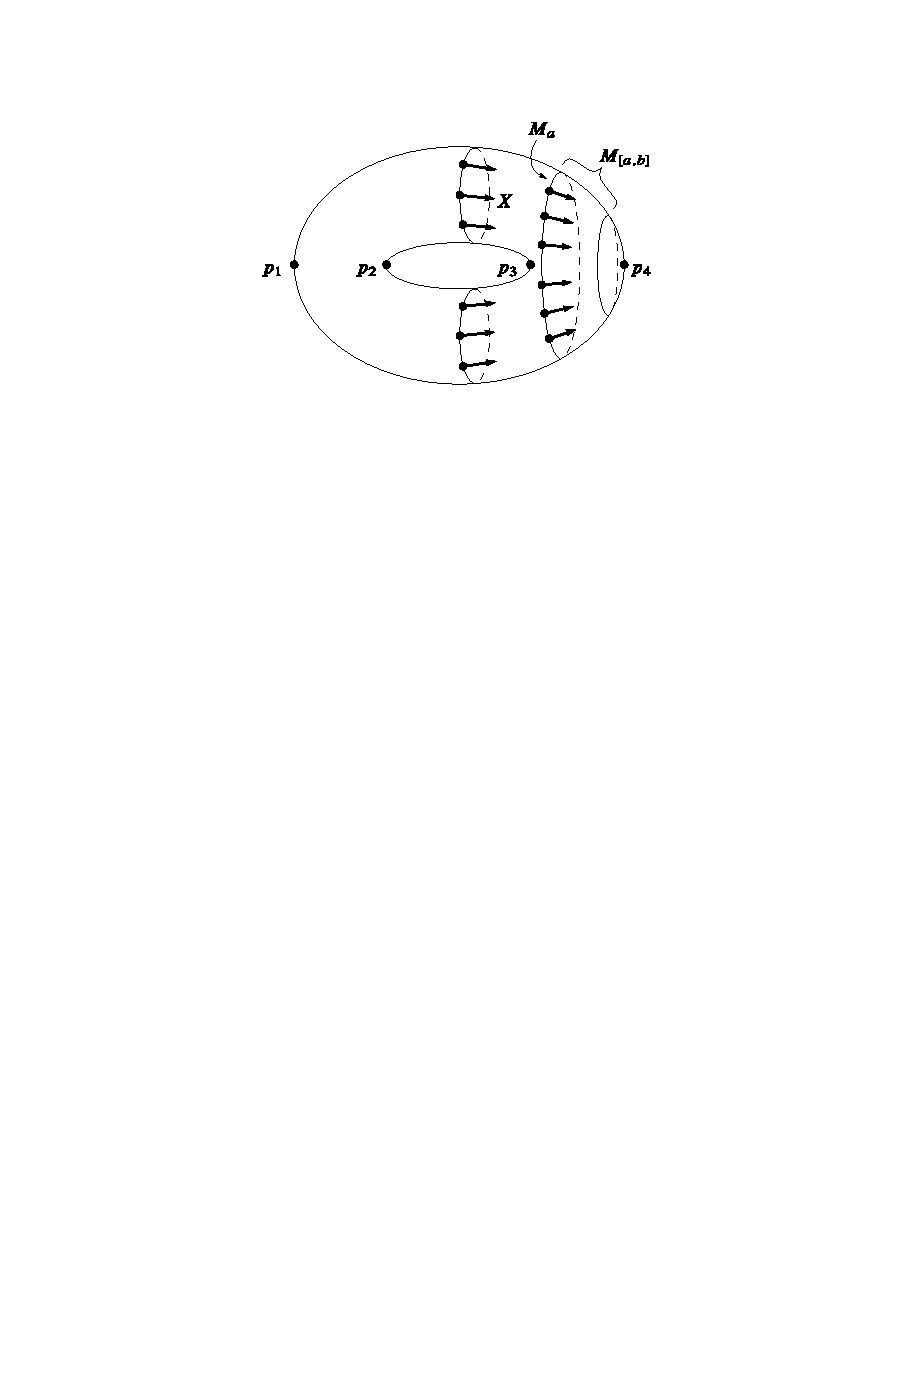
\includegraphics{pictures/Morse-setup}
\caption{The setup for Exercise~\ref{Morse exercise}.}
\end{figure}
\begin{proof}
Fix a point $p\in M\setminus\{p_1,\dots,p_k\}$, we calculate the derivative of $f(\theta_t(p))$ with respect to $t$. We have
\[d(f\circ\theta_t(p))=df\circ d(\theta_t(p))=df(X_{\theta_t(p)})=\langle \grad f|_{\theta_t(p)},X_{\theta_t(p)}\rangle=1.\]
Therefore 
\begin{align}\label{Morse exercise-1}
f(\theta_t(p))=f(\theta_0(p))+t=f(p)+t
\end{align}

Now let $p\in M_a$, we observe that
\begin{align*}
f(\theta_t(p))=f(p)+t=a+t.
\end{align*}
Therefore $\theta$ restricts to a map $\theta|_{M_{[a,b]}}:[0,b-a]\times M_a\to M_{[a,b]}$. To show this is a diffeomorphism, we construct the inverse map of $\theta|_{M_{[a,b]}}$:
\[\psi:M_{[a,b]}\to[0,b-a]\times M_a,\quad p\mapsto(f(p)-a,\theta_{a-f(p)}(p)).\]
Note that since $M_{[a,b]}$ is compact ($M$ is compact and $M_{[a,b]}$ is closed), the integral curve passing $p$ is defined on $\R$ if it is contained in $M_{[a,b]}$ by the escape lemma 
(Lemma~\ref{vector flow escape lemma}). But from equation $(\ref{Morse exercise-1})$, this is impossible. So it must pass the boundary of $M_{[a,b]}$, i.e., threr 
is $t_0\in\R$ such that $\theta_t(p)\in M_a$. We can see $t_0=a-f(p)$ from $(\ref{Morse exercise-1})$, so our definition of $\psi$ is legal. Now it is easy to see that 
$\psi$ is the inverse of $\theta|_{M_{[a,b]}}$, so we get the diffeomorphism.
\end{proof}
\section{Differential forms}
\subsection{The alternating tensors}
We continue to assume that $V$ is a finite-dimensional real vector space. A covariant $k$-tensor $\alpha$ on $V$ is said to be alternating (or antisymmetric or skew-symmetric) if it changes sign whenever two of its arguments are interchanged. This means that for all vectors $v_1,\dots,v_k$ and every pair of distinct indices $i,j$ it satisfies
\[\alpha(v_1,\dots,v_i,\dots,v_j,\dots,v_k)=-\alpha(v_1,\dots,v_j,\dots,v_i,\dots,v_k).\]
Alternating covariant $k$-tensors are also variously called \textbf{exterior forms}, \textbf{multicovectors}, or \textbf{$\bm{k}$-covectors}. The subspace of all alternating covariant $k$-tensors on $V$ is denoted by $\bigwedge^k(V^*)\sub T^k(V^*)$.\par
The next lemma gives two more useful characterizations of alternating tensors.
\begin{lemma}\label{alt tensor lem}
Let $\alpha$ be a covariant $k$-tensor on a finite-dimensional vector space $V$. The following are equivalent:
\begin{itemize}
\item[(a)] $\alpha$ is alternating.
\item[(b)] $\alpha(v_1,\dots,v_k)=0$ whenever the $k$-tuple $v_1,\dots,v_k$ is linearly dependent.
\item[(c)] $\alpha$ gives the value zero whenever two of its arguments are equal:
\[\alpha(v_1,\dots,w,\dots,w,v_k)=0.\]
\end{itemize}
\end{lemma}
\begin{proof}
The implications $(a)\Rightarrow(c)$ and $(b)\Rightarrow(c)$ are immediate. We complete the proof by showing that (c) implies both (a) and (b).\par
Assume that $\alpha$ satisfies (c). For any vectors $v_1,\dots,v_k$, the hypothesis implies
\begin{align*}
0&=\alpha(v_1,\dots,v_i+v_j,\dots,v_i+v_j,\dots,v_k)\\
&=\alpha(v_1,\dots,v_i,\dots,v_j,\dots,v_k)+(v_1,\dots,v_j,\dots,v_i,\dots,v_k).
\end{align*}
Thus $\alpha$ is alternating. On the other hand, if $v_1,\dots,v_k$ is a linearly dependent $k$-tuple, then one of the $v_i$'s can be written as a linear combination of the others. For simplicity, let us assume that $v_k=\sum_{j=1}^{k-1}a^jv_j$. Then multilinearity of $\alpha$ implies
\[\alpha(v_1,\dots,v_k)=\sum_{j=1}^{k-1}a^j\alpha(v_1,\dots,v_{k-1},v_j).\]
In each of these terms, $\alpha$ has two identical arguments, so every term is zero.
\end{proof}
We now define a similar projection $\Alt:T^k(V^*)\to\bigwedge^k(V^*)$, called \textbf{alternation}, as follows:
\[\Alt\alpha=\frac{1}{k!}\sum_{\sigma\in\mathfrak{S}_k}(-1)^\sigma\sigma\cdot\alpha.\]
More explicitly, this means
\[\Alt\alpha(v_1,\dots,v_k)=\frac{1}{k!}\sum_{\sigma\in\mathfrak{S}_k}(\sgn\sigma)\alpha(v_{\sigma(1)},\dots,v_{\sigma(k)}).\]
\begin{example}
If $\alpha$ is any $1$-tensor, then $\Alt\alpha=\alpha$. If $\alpha$ is a $2$-tensor, then
\[(\Alt\alpha)(v,w)=\frac{1}{2}\big(\alpha(v,w)-\alpha(w,v)\big).\]
\end{example}
The next proposition is the analogue for alternating tensors of Proposition~\ref{symmetrization prop}.
\begin{proposition}
Let $\alpha$ be a covariant tensor on a finite-dimensional vector space.
\begin{itemize}
\item[(a)] $\Alt\alpha$ is alternating.
\item[(b)] $\Alt\alpha=\alpha$ if and only if $\alpha$ is alternating.
\end{itemize}
\end{proposition}
\subsubsection{Elementary alternating tensors}
For computations with alternating tensors, the following notation is exceedingly useful. Given a positive integer $k$, an ordered $k$-tuple $I=(i_1,\dots,i_k)$ of positive integers is called a \textbf{multi-index of length $\bm{k}$}. If $I$ is such a multi-index and $\sigma\in\mathfrak{S}_k$ is a permutation, we write $I_\sigma$ for the following multi-index:
\[I_\sigma=(i_{\sigma(1)},\dots,i_{\sigma(k)}).\]
Note that $I_{\tau\sigma}=(I_{\sigma})_\tau$ for $\sigma,\tau\in\mathfrak{S}_k$.\par
Let $V$ be an $n$-dimensional vector space, and suppose $(\eps^1,\dots,\eps^n)$ is any basis for $V^*$. We now define a collection of $k$-covectors on $V$ that generalize the determinant function on $\R^n$. For each multi-index $I=(i_1,\dots,i_k)$ of length $k$ such that $1\leq i_1<\dots<i_k\leq n$, define a covariant $k$-tensor
\begin{align}\label{elementry alt tensor}
\eps^I(v_1,\dots,v_k)=\det\begin{pmatrix}
\eps^{i_1}(v_1)&\cdots&\eps^{i_1}(v_k)\\
\vdots&\ddots&\vdots\\
\eps^{i_k}(v_1)&\cdots&\eps^{i_k}(v_k)
\end{pmatrix}=\det\begin{pmatrix}
v_1^{i_1}&\cdots&v_k^{i_1}\\
\vdots&\ddots&\vdots\\
v_1^{i_k}&\cdots&v_k^{i_k}
\end{pmatrix}
\end{align}
In other words, if $V$ denotes the $n\times k$ matrix whose columns are the components of the vectors $v_1,\dots,v_k$ with respect to the basis $(E_i)$ dual to $(\eps^i)$, then $\eps^I(v_1,\dots,v_k)$ is the determinant of the $k\times k$ submatrix consisting of rows $i_1,\dots,i_k$ of $V$. Because the determinant changes sign whenever two columns are interchanged, it is clear that $\eps^I$ is an alternating $k$-tensor. We call $\eps^I$ an \textbf{elementary alternating tensor} or \textbf{elementary $\bm{k}$-covector}.
\begin{example}
In terms of the standard dual basis $(e^1,e^2,e^3)$ for $(\R^3)^*$, we have
\[e^{13}(v,w)=v^1w^3-w^1v^3;\]
\[e^{123}(v,w,x)=\det(v,w,x).\]
\end{example}
In order to streamline computations with the elementary $k$-covectors, it is useful to extend the Kronecker delta notation in the following way. If $I$ and $J$ are multiindices of length $k$, we define
\[\delta^I_J=\det\begin{pmatrix}
\delta^{i_1}_{j_1}&\cdots&\delta^{i_1}_{j_k}\\
\vdots&\ddots&\vdots\\
\delta^{i_k}_{j_1}&\cdots&\delta^{i_k}_{j_k}
\end{pmatrix}\]
so that
\[\delta^I_J=\begin{cases}
\sgn\sigma&\text{if neither $I$ nor $J$ has a repeated index and $J=I$ for some $\sigma\in\mathfrak{S}_k$,}\\
0&\text{if $I$ or $J$ has a repeated index or $J$ is not a permutation of $I$.}
\end{cases}\]
\begin{lemma}[\textbf{Properties of Elementary $\bm{k}$-Covectors}]\label{alt elementry prop}\label{alt ele prop}
Let $(E_i)$ be a basis for $V$, let $(\eps^i)$ be the dual basis for $V^*$, and let $\eps^I$ be as defined above.
\begin{itemize}
\item[(a)] If $I$ has a repeated index, then $\eps^I=0$.
\item[(b)] If $J=I_\sigma$ for some $\sigma\in\mathfrak{S}_k$, then $\eps^J=\sgn\sigma\eps^I$.
\item[(c)] The result of evaluating $\eps^I$ on a sequence of basis vectors is
\[\eps^I(E_{j_1},\dots,E_{j_k})=\delta^I_J.\]
\end{itemize}
\end{lemma}
The significance of the elementary $k$-covectors is that they provide a convenient basis for $\bigwedge^k(V^*)$. Of course, the $\eps^I$'s are not all linearly independent, because some of them are zero and the ones corresponding to different permutations of the same multi-index are scalar multiples of each other. But as the next proposition shows, we can get a basis by restricting attention to an appropriate subset of multi-indices. A multi-index $I=(i_1,\dots,i_k)$ is said to be \textbf{increasing} if $i_1<\cdots<i_k$. It is useful to use a primed summation sign to denote a sum over only increasing multi-indices, so that, for example,
\[\sum'_I\alpha_I\eps^I:=\sum_{i_1<\cdots<i_k}\alpha_I\eps^I.\]
\begin{proposition}[\textbf{A Basis for $\bm{\bigwedge^k(V^*)}$}]\label{alt tensor basis}
Let $V$ be an n-dimensional vector space. If $(\eps^i)$ is any basis for $V^*$, then for each positive integer $k\leq n$, the collection of $k$-covectors
\[\mathcal{E}:=\{\eps^I:\text{$I$ is an increasing multi-index of length $k$}\}\]
is a basis for $\bigwedge^k(V^*)$. Therefore,
\[\dim\bigwedge\nolimits^k(V^*)=\binom{n}{k}.\]
If $k>n$, then $\dim\bigwedge^k(V^*)=0$.
\end{proposition}
In particular, for an $n$-dimensional vector space $V$, this proposition implies that $\bigwedge^n(V^*)$ is $1$-dimensional and is spanned by $\eps^{1\dots n}$. By definition, this elementary $n$-covector acts on vectors $v_1,\dots,v_n$ by taking the determinant of their component matrix $V=(v_j^i)$. For example, on $\R^n$ with the standard basis, $e^{1\dots n}$ is precisely the determinant function.\par
One consequence of this is the following useful description of the behavior of an
$n$-covector on an $n$-dimensional space under linear maps. Recall that if $T:V\to V$
is a linear map, the determinant of $T$ is defined to be the determinant of the matrix representation of $T$ with respect to any basis.
\begin{proposition}\label{alt n tensor linear map}
Suppose $V$ is an $n$-dimensional vector space and $\omega\in\bigwedge^n(V^*)$. If $T:V\to V$ is any linear map and $v_1,\dots,v_n$ are arbitrary vectors in $V$, then
\begin{align}\label{alt n tensor linear map-1}
\omega(Tv_1,\dots,Tv_n)=(\det T)\omega(v_1,\dots,v_n).
\end{align}
\end{proposition}
\begin{proof}
Let $(E_i)$ be any basis for $V$, and let $(\eps^i)$ be the dual basis. Let $(T_i^j)$ denote the matrix of $T$ with respect to this basis, and let $T_i=TE_i=T_i^jE_j$ 
be the $i$-th column of $T$. By Proposition~\ref{alt tensor basis}, we can write $\omega=\lambda\,\eps^{1\dots n}$ for some real number $\lambda$.\par
Since both sides of $(\ref{alt n tensor linear map-1})$ are multilinear functions of $v_1,\dots,v_n$, it suffices to verify the identity when the $v_i$'s are basis 
vectors. Furthermore, since both sides are alternating, we only need to check the case $(v_1,\dots,v_n)=(E_1,\dots,E_n)$. In this case, the right-hand side of 
$(\ref{alt n tensor linear map-1})$ is
\[(\det T)\lambda\,\eps^{1\dots n}(E_1,\dots,E_n)=\lambda\det T.\]
On the other hand, the left-hand side reduces to
\[\omega(TE_1,\dots,TE_n)=\lambda\,\eps^{1\dots n}(T_1,\dots,T_n)=\lambda\,\det(T_i^j),\]
which is equal to the right-hand side.
\end{proof}
\subsubsection{The wedge product}
We continue with the assumption that $V$ is a finite-dimensional real vector space.
Given $\omega\in\bigwedge^k(V^*)$ and $\eta\in\bigwedge^l(V^*)$, we define their wedge product or exterior product to be the following $(k+l)$-covector:
\begin{align}\label{wedge product def}
\omega\wedge\eta=\frac{(k+l)!}{k!l!}\Alt(\omega\otimes\eta).
\end{align}
The mysterious coefficient is motivated by the simplicity of the statement of the
following lemma.
\begin{lemma}\label{wedge prod form}
Let $V$ be an $n$-dimensional vector space and let $(e^1,\dots,e^n)$ be a basis for $V^*$. For any multi-indices $I=(i_1,\dots,i_k)$ and $J=(j_1,\dots,j_l)$,
\begin{align}\label{wedge product ele form-1}
\eps^I\wedge\eps^J=\eps^{IJ},
\end{align}
where $I=(i_1,\dots,i_k,j_1,\dots,j_l)$ is obtained by concatenating $I$ and $J$.
\end{lemma}
\begin{proof}
By multilinearity, it suffices to show that
\begin{align}\label{wedge product ele form-2}
\eps^I\wedge\eps^J(E_{p_1},\dots,E_{p_{k+l}})=\eps^{IJ}(E_{p_1},\dots,E_{p_{k+l}})
\end{align}
for any sequence $(E_{p_1},\dots,E_{p_{k+l}})$ of basis vectors. We consider several cases.
\begin{itemize}
\item Case $1$: $P=(p_1,\dots,p_{k+l})$ has a repeated index. In this case, both sides of $(\ref{wedge product ele form-2})$ are zero by Lemma~\ref{alt tensor lem}(c).
\item Case $2$: $P$ contains an index that does not appear in either $I$ or $J$. In this case, the right-hand side is zero by Lemma~\ref{alt elementry prop}(c). Similarly, each term in the expansion of the left-hand side involves either $\eps^I$ or $\eps^J$ evaluated on a sequence of basis vectors that is not a permutation of $I$ or $J$, respectively, so the left-hand side is also zero.
\item Case $3$: $P=IJ$ and $P$ has no repeated indices. In this case, the right-hand side of $(\ref{wedge product ele form-2})$ is equal to $1$ by Lemma~\ref{alt ele prop}(c), so we need to show that the left-hand side is also equal to $1$. By definition,
\begin{align*}
\eps^I\wedge\eps^J(E_{p_1},\dots,E_{p_{k+l}})&=\frac{(k+l)!}{k!l!}\Alt(\eps^I\otimes\eps^J)(E_{p_1},\dots,E_{p_{k+l}})\\
&=\frac{1}{k!l!}\sum_{\sigma\in\mathfrak{S}_{k+l}}(\sgn\sigma)\eps^I(E_{p_{\sigma(1)}},\dots,E_{p_{\sigma(k)}})\eps^J(E_{p_{\sigma(k+1)}},\dots,E_{p_{\sigma(k+l)}})
\end{align*}
By Lemma~\ref{alt ele prop} again, the only terms in the sum above that give nonzero values are those in which $\sigma$ permutes the first $k$ indices and the last $l$ indices of $P$ separately. In other words, $\sigma$ must split into $\sigma=\tau\eta$, where $\tau\in\mathfrak{S}_k$ acts by permuting $\{1,\dots,k\}$ and $\eta\in\mathfrak{S}_l$ acts by permuting $\{k+1,\dots,k+l\}$. Since $\sgn(\tau\eta)=(\sgn\tau)(\sgn\eta)$, we have
\begin{align*}
&\eps^I\wedge\eps^J(E_{p_1},\dots,E_{p_{k+l}})\\
&=\frac{1}{k!l!}\sum_{\tau\in\mathfrak{S}_{k},\eta\in\mathfrak{S}_l}(\sgn\tau)(\sgn\eta)\eps^I(E_{p_{\tau(1)}},\dots,E_{p_{\tau(k)}})\eps^J(E_{p_{\eta(k+1)}},\dots,E_{p_{\eta(k+l)}})\\
&=\Big(\frac{1}{k!}\sum_{\tau\in\mathfrak{S}_{k}}(\sgn\tau)\eps^I(E_{p_{\tau(1)}},\dots,E_{p_{\tau(k)}})\Big)\Big(\frac{1}{l!}\sum_{\eta\in\mathfrak{S}_{l}}(\sgn\eta)\eps^J(E_{p_{\eta(k+1)}},\dots,E_{p_{\eta(k+l)}})\Big)\\
&=(\Alt\eps^I)(E_{p_1},\dots,E_{p_k})(\Alt\eps^J)(E_{p_{k+1}},\dots,E_{p_{k+l}})\\
&=\eps^I(E_{p_1},\dots,E_{p_k})\eps^J(E_{p_{k+1}},\dots,E_{p_{k+l}})=1.
\end{align*}
\item Case $4$: $P$ is a permutation of $IJ$ and has no repeated indices. In this case, applying a permutation to $P$ brings us back to Case $3$. Since the effect of the permutation is to multiply both sides of $(\ref{wedge product ele form-2})$ by the same sign, the result holds in this case as well.
\end{itemize}
\end{proof}
\begin{proposition}[\textbf{Properties of the Wedge Product}]\label{wedge prod prop}
Suppose $\omega,\omega',\eta,\eta'$ and $\xi$ are multicovectors on a finite-dimensional vector space $V$.
\begin{itemize}
\item[(a)] Bilinearity: For $a,a'\in\R$,
\begin{flalign*}
&(a\omega+a'\omega')\wedge\eta=a(\omega\wedge\eta)+a'(\omega'\wedge\eta),\\
&\eta\wedge(a\omega+a'\omega')=a(\eta\wedge\omega)+a'(\eta\wedge\omega').
\end{flalign*}
\item[(b)] Associativity:
\[(\omega\wedge\eta)\wedge\xi=\omega\wedge(\eta\wedge\xi).\]
\item[(c)] Anticommutativity: For $\omega\in\bigwedge^k(V^*)$ and $\eta\in\bigwedge^l(V^*)$,
\begin{align}\label{wedge prod prop-1}
\omega\wedge\eta=(-1)^{kl}\eta\wedge\omega.
\end{align}
\item[(d)] If $(\eps^i)$ is any basis for $V^*$ and $I=(i_1,\dots,i_k)$ is any multi-index, then
\begin{align}\label{wedge prod prop-2}
\eps^{i_1}\wedge\cdots\wedge\eps^{i_k}=\eps^I.
\end{align}
\item[(e)] For any covectors $i_1,\dots,i_k$ and vectors $v_1,\dots,v_k$
\begin{align}\label{wedge prod prop-3}
\omega_1\wedge\cdots\wedge\omega_k(v_1,\dots,v_k)=\det\big(\omega^j(v_i)\big).
\end{align}
\end{itemize}
\end{proposition}
\begin{proof}
Bilinearity follows immediately from the definition, because the tensor product is bilinear and Alt is linear. To prove associativity, note that Lemma~\ref{wedge prod form} gives
\[(\eps^I\wedge\eps^J)\eps^K=\eps^{IJK}=\eps^I\wedge(\eps^I\wedge\eps^J).\]
The general case follows from bilinearity. Similarly, using Lemma~\ref{wedge prod form} again, we get
\[\eps^I\wedge\eps^J=\eps^{IJ}=(\sgn\tau)\eps^{JI}=(\sgn\tau)\eps^{J}\wedge\eps^{I},\]
where $\tau$ is the permutation that sends $IJ$ to $JI$. It is easy to check that $\sgn\tau=(-1)^{kl}$, because $\tau$ can be decomposed as a composition of $kl$ transpositions. Anticommutativity then follows from bilinearity.\par
Part (d) is an immediate consequence of Lemma~\ref{wedge prod form} and induction. To prove (e), we note that the special case in which each $\omega^j$ is one of the basis covectors $\eps^{i_j}$ reduces to $(\ref{wedge prod prop-2})$. Since both sides of $(\ref{wedge prod prop-3})$ are multilinear in $(\omega_1,\dots,\omega_k)$, this suffices.
\end{proof}
Because of part (d) of this lemma, henceforth we generally use the notations $\eps^I$ and $\eps^{i_1}\wedge\cdots\wedge\eps^{i_k}$ interchangeably.\par
A $k$-covector $\omega$ is said to be decomposable if it can be expressed in the form $\omega^{1}\wedge\cdots\wedge\omega^k$, where $\omega^1,\dots,\omega^k$ are covectors. It is important to be aware that not every $k$-covector is decomposable when $k>1$; however, it follows from Propositions~\ref{alt tensor basis} and ~\ref{wedge prod prop}(d) that every $k$-covector can be written as a linear combination of decomposable ones.\par
The definition and computational properties of the wedge product can seem daunting at first sight. However, the only properties that you need to remember for most practical purposes are the ones expressed in the preceding proposition. In fact,
these properties are more than enough to determine the wedge product uniquely, as
the following proposition shows.
\begin{proposition}
The wedge product is the unique associative, bilinear, and anticommutative map $\bigwedge^k(V^*)\times\bigwedge^k(V^*)\to\bigwedge^{k+l}(V^*)$ satisfying $(\ref{wedge prod prop-2})$.
\end{proposition}
For any $n$-dimensional vector space $V$, define a vector space $\bigwedge(V^*)$ by
\[\bigwedge(V^*)=\bigoplus_{k=0}^{n}\bigwedge\nolimits^k(V^*).\]
It follows from Proposition~\ref{alt tensor basis} that $\dim\bigwedge(V^*)=2^n$. Proposition~\ref{wedge prod prop} shows that the wedge product turns $\bigwedge(V^*)$ into an associative algebra, called the \textbf{exterior algebra} (or \textbf{Grassmann algebra}) of $V$. This algebra is not commutative, but it has
a closely related property. An algebra $A$ is said to be graded if it has a direct sum decomposition $A=\bigoplus_kA^k$ such that the product satisfies $A^kA^l\sub A^{k+l}$ for each $k$ and $l$. A graded algebra is anticommutative if the product satisfies $ab=(-1)^{kl}ba$ for $a\in A^k$, $b\in A^l$. Proposition~\ref{wedge prod prop}(c) shows that $\bigwedge(V^*)$ is an anticommutative graded algebra.
\subsubsection{Interior multiplication}
There is an important operation that relates vectors with alternating tensors. Let $V$ be a finite-dimensional vector space. For each $v\in V$, we define a linear map $i_v:\bigwedge^k(V^*)\to\bigwedge^{k-1}(V^*)$, called \textbf{interior multiplication by $\bm{v}$}, as follows:
\[i_v\omega(w_1,\dots,w_{k-1})=\omega(v,w_1,\dots,w_{k-1}).\]
In other words, $i_v\omega$ is obtained from $\omega$ by inserting $v$ into the first slot. By convention, we interpret $i_v\omega$ to be zero when $\omega$ is a $0$-covector (i.e., a number). Another common notation is $v\intprod\omega=i_v\omega$.
\begin{lemma}\label{interior multiplication lem}
Let $V$ be a finite-dimensional vector space and $v\in V$
\begin{itemize}
\item[(a)] $i_v\circ i_v=0$.
\item[(b)] If $\omega\in\bigwedge^k(V^*)$ and $\eta\in\bigwedge^l(V^*)$,
\begin{align}\label{interior multiplication-1}
i_v(\omega\wedge\eta)=(i_v\omega)\wedge\eta+(-1)^k\omega\wedge(i_v\eta).
\end{align}
\end{itemize} 
\end{lemma}
\begin{proof}
On $k$-covectors for $k\geq2$, part (a) is immediate from the definition, because any alternating tensor gives zero when two of its arguments are identical. On $1$-covectors and $0$-covectors, it follows from the fact that $i_v\equiv0$ on $0$-covectors.\par
To prove (b), it suffices to consider the case in which both $\omega$ and $\eta$ are decomposable, since every alternating tensor of positive rank can be written as a linear combination of decomposable ones. It is straightforward to verify that (b) follows in this special case from the following general formula for covectors $\omega^1,\dots,\omega^k$:
\begin{align}\label{interior multiplication-2}
v\intprod(\omega^1\wedge\cdots\omega^k)=\sum_{i=1}^{k}(-1)^{i-1}\omega^i(v)\omega^1\wedge\cdots\wedge\widehat{\omega^i}\wedge\cdots\wedge\omega^k
\end{align}
To prove this, let us write $v_1=v$ and apply both sides to an arbitrary $(k-1)$-tuple of vectors $(v_2,\dots,v_k)$ then what we have to prove is 
\begin{align}\label{interior multiplication-3}
v\intprod(\omega^1\wedge\cdots\omega^k)(v_1,\dots,v_k)=\sum_{i=1}^{k}(-1)^{i-1}\omega^i(v_1)(\omega^1\wedge\cdots\wedge\widehat{\omega^i}\wedge\cdots\wedge\omega^k)(v_2,\dots,v_k).
\end{align}
The left-hand side of $(\ref{interior multiplication-3})$ is the determinant of the matrix $V$ whose $(i,j)$-entry is $\omega^i(v_j)$. To simplify the right-hand side, let $V^i_j$ denote the $(k-1)\times(k-1)$ submatrix of $V$ obtained by deleting the $i$ th row and $j$ th column. Then the right-hand side of $(\ref{interior multiplication-3})$ is
\[\sum_{i=1}^{k}(-1)^{i-1}\omega^i(v_1)V^i_1.\]
This is just the expansion of $\det V$ by minors along the first column, and therefore is equal to $\det V$.
\end{proof}
\subsection{Differential forms on manifolds}
Now we turn our attention to an $n$-dimensional smooth manifold $M$ (with or without boundary). Recall that $T^kT^*M$ is the bundle of covariant $k$-tensors on $M$. The subset of $T^kT^*M$ consisting of alternating tensors is denoted by
\[\bigwedge\nolimits^kT^*M=\prod_{p\in M}\bigwedge\nolimits^k(T^*_pM).\]
A section of $\bigwedge^kT^*M$ is called a \textbf{differential $\bm{k}$-form}, or just a \textbf{$\bm{k}$-form}; this is a (continuous) tensor field whose value at each point is an alternating tensor. The integer $k$ is called the degree of the form. We denote the vector space of smooth $k$-forms by
\[\Omega^k(M):=\Gamma(\bigwedge\nolimits^kT^*M).\]
The wedge product of two differential forms is defined pointwise: $(\omega\wedge\eta)_p=\omega_p\wedge\eta_p$. Thus, the wedge product of a $k$-form with an $l$-form is a $(k+l)$-form. If $f$ is a $0$-form and $\omega$ is a $k$-form, we interpret the wedge product $f\wedge\omega$ to mean the ordinary product $f\omega$. If we define 
\begin{align*}
\Omega^*(M)=\bigoplus_{k=0}^{n}\Omega^k(M),
\end{align*}
then the wedge product turns $\Omega^*(M)$ into an associative, anticommutative graded algebra.\par 
In any smooth chart, a $k$-form $\omega$ can be written locally as
\[\omega=\sum_{I}'\omega_I\,dx^{i_1}\wedge\cdots\wedge dx^{i_k}=\sum_{I}'\omega_I\,dx^I.\]
Proposition~\ref{tensor field smooth crit} shows that $\omega$ is smooth on $U$ if and only if the component functions $\omega^I$ are smooth. In terms of differential forms, the result of Lemma~\ref{alt ele prop}(c) translates to
\[dx^{i_1}\wedge\cdots\wedge dx^{i_k}\Big(\frac{\partial}{\partial x^{j_1}},\dots,\frac{\partial}{\partial x^{j_k}}\Big)=\delta^I_J.\]
Thus the component functions $\omega_I$ of $\omega$ are determined by
\[\omega_I=\omega\Big(\frac{\partial}{\partial x^{i_1}},\dots,\frac{\partial}{\partial x^{i_k}}\Big).\]
\begin{example}
A $0$-form is just a continuous real-valued function, and a $1$-form is a covector field. On $\R^3$, some examples of smooth $2$-forms are given by
\[\omega=(\sin xy)\,dy\wedge dz,\quad\eta=dx\wedge dy+dy\wedge dz+ dz\wedge dx.\]
Every $3$-form on $\R^3$ is a continuous real-valued function times $dx\wedge dy\wedge dz$.
\end{example}
If $F:M\to N$ is a smooth map and $\omega$ is a differential form on $N$, the pullback $F^*\omega$ is a differential form on $M$, defined as for any covariant tensor field:
\[(F^*\omega)_p(v_1,\dots,v_k)=\omega_p\big(dF_p(v_1),\dots,dF_p(v_k)\big).\]
\begin{lemma}\label{form pull back formula}
Suppose $F:M\to N$ is smooth.
\begin{itemize}
\item[(a)] $F^*:\Omega^k(N)\to\Omega^k(M)$ is linear over $\R$.
\item[(b)] $F^*(\omega\wedge\eta)=(F^*\omega)\wedge(F^*\eta)$.
\item[(c)] In any smooth chart,
\[F^*\Big(\sum'_{I}\omega_I\,dy^{i_1}\wedge\cdots\wedge dy^{i_k}\Big)=\sum'_{I}(\omega_I\circ F)\,d(y^{i_1}\circ F)\wedge\cdots\wedge d(y^{i_k}\circ F).\]
\end{itemize}
\end{lemma}
This lemma gives a computational rule for pullbacks of differential forms similar to the ones we developed for covector fields and arbitrary tensor fields earlier.
\begin{example}
Define $F:\R^2\to\R^3$ by $F(u,v)=(u,v,u^2-v^2)$, and let $\omega$ be the $2$-form $y\,dx\wedge dz+x\,dy^dz$ on $\R^3$. The pullback $F^*\omega$ is computed as follows:
\begin{align*}
F^*(y\,dx\wedge dz+x\,dy^dz)&=v\,du\wedge d(u^2-v^2)+u\,dv\wedge d(u^2-v^2)\\
&=v\,du\wedge(2u\,du-2v\,dv)+u\,dv\wedge(2u\,du-2v\,dv)\\
&=-2v^2\,du\wedge dv+2u^2\,dv\wedge du\\
&=-2(u^2+v^2)\,du\wedge dv.
\end{align*}
\end{example}
The same technique can also be used to compute the expression for a differential form in another smooth chart.
\begin{example}
Let $\omega=dx\wedge dy$ on $\R^2$. Thinking of the transformation to polar coordinates $x=r\cos\theta$, $y=r\sin\theta$ as an expression for the identity map with
respect to different coordinates on the domain and codomain, we obtain
\begin{align*}
dx\wedge dy&=d(r\cos\theta)\wedge d(r\sin\theta)=(\cos\theta\,dr-r\sin\theta d\theta)\wedge(\sin\theta\,dr+r\cos\theta\,d\theta)=r\,dr\wedge d\theta.
\end{align*}
\end{example}
The similarity between this formula and the formula for changing a double integral from Cartesian to polar coordinates is striking. The following proposition
generalizes this.
\begin{proposition}[\textbf{Pullback Formula for Top-Degree Forms}]\label{pull back n form}
Let $F:M\to N$ be a smooth map between $n$-manifolds with or without boundary. If $(x^i)$ and $(y^j)$ are smooth coordinates on open subsets $U\sub M$ and $V\sub N$, respectively, and $u$ is a continuous real-valued function on $V$, then the following holds on $U\cap F^{-1}(V)$:
\begin{align}\label{pull back n form-1}
F^*(u\,dy^1\wedge\cdots\wedge dy^n)&=(u\circ F)(\det\partial F)\,dx^1\wedge\cdots\wedge dx^n.
\end{align}
where $\partial F$ represents the Jacobian matrix of $F$ in these coordinates.
\end{proposition}
\begin{proof}
Because the fiber of $\bigwedge^nT^*M$ is spanned by $dx^1\wedge\cdots\wedge dx^n$ at each point, it suffices to show that both sides of $(\ref{pull back n form-1})$ give the same result when evaluated on $(\partial/\partial x^1,\dots,\partial/\partial x^n)$. From Lemma~\ref{form pull back formula},
\[F^*(u\,dy^1\wedge\cdots\wedge dy^n)=(u\circ F)\,dF^1\wedge\cdots\wedge dF^n.\]
Proposition~\ref{wedge prod prop}(d) shows that
\[dF^1\wedge\cdots\wedge dF^n\Big(\frac{\partial}{\partial x^1},\dots,\frac{\partial}{\partial x^n}\Big)=\det\Big(\frac{\partial F^j}{\partial x^i}\Big).\]
Therefore, the left-hand side of $(\ref{pull back n form-1})$ gives $(u\circ F)(\det\partial F)$ when applied to $(\partial/\partial x^1,\dots,\partial/\partial x^n)$. On the other hand, the right-hand side gives the same thing, because $dx^1\wedge\cdots\wedge dx^n(\partial/\partial x^1,\dots,\partial/\partial x^n)=1$.
\end{proof}
\begin{corollary}
If $(U,(x^i))$ and $(\widetilde{U},(\widetilde{x}^j))$ are overlapping smooth coordinate charts on $M$, then the following identity holds on $U\cap\widetilde{U}$:
\begin{align}\label{form n transition}
d\widetilde{x}^1\wedge\cdots\wedge d\widetilde{x}^i=\det\Big(\frac{\partial\widetilde{x}^j}{\partial x^i}\Big)dx^1\wedge\cdots\wedge dx^n.
\end{align}
\end{corollary}
Interior multiplication also extends naturally to vector fields and differential forms, simply by letting it act pointwise: if $X\in\X(M)$ and $\omega\in\Omega^k(M)$, define a $(k-1)$-form $X\intprod\omega=i_X\omega$ by
\[(X\intprod\omega)_X=X_p\intprod\omega_p.\]
The following results are clear.
\begin{proposition}
Let $X$ be a smooth vector field on $M$.
\begin{itemize}
\item[(a)] If $\omega$ is a smooth differential form, then $i_X\omega$ is smooth.
\item[(b)] The map $i_X:\Omega^k(M)\to\Omega^{k-1}(M)$ is linear over $C^\infty(M)$, therefore corresponds
to a smooth bundle homomorphism $i_X:\bigwedge^kT^*M\to\bigwedge^{k-1}T^*M$.
\end{itemize}
\end{proposition}
\subsection{Exterior derivatives}
For each smooth manifold $M$ with or without boundary, we will show that there is a differential operator $d:\Omega^k(M)\to\Omega^{k+1}(M)$ satisfying $d(d\omega)=0$ for all $\omega$. Thus, it will follow that a necessary condition for a smooth $k$-form $\omega$ to be equal to $d\omega$ for some $(k-1)$-form $\omega$ is that $d\omega=0$.\par 
The definition of $d$ on Euclidean space is straightforward: if $\omega=\sum'_J\omega_J\,dx^J$ is a smooth $k$-form on an open subset $U\sub\R^n$ or $\H^n$, we define its exterior derivative $d\omega$ to be the following $(k+1)$-form:
\begin{align}\label{ext der R^n}
d\omega=\sum'_Jd\omega_J\wedge dx^J,
\end{align}
where $d\omega_J$ is the differential of the function $\omega_J$. In somewhat more detail, this is
\[d\Big(\sum'_J\omega_J\,dx^{j_1}\wedge\cdots\wedge dx^{j_k}\Big)=\sum'_J\sum_{i}\frac{\partial\omega_J}{\partial x^i}dx^i\wedge dx^{j_1}\wedge\cdots\wedge dx^{j_k}.\]
In order to transfer this definition to manifolds, we need to check that it satisfies the following properties.
\begin{proposition}[\textbf{Properties of the Exterior Derivative on $\bm{\R^n}$}]\label{ext der R^n prop}
\mbox{}
\begin{itemize}
\item[(a)] $d$ is linear over $\R$.
\item[(b)] If $\omega$ is a smooth $k$-form and $\eta$ is a smooth $l$-form on an open subset $U\sub\R^n$ or $\H^n$, then
\[d(\omega\wedge\eta)=d\omega\wedge\eta+(-1)^k\omega\wedge d\eta.\]
\item[(c)] $d\circ d\equiv0$.
\item[(d)] $d$ commutes with pullbacks: if $U$ is an open subset of $\R^n$ or $\H^n$, $V$ is an open subset of $\R^m$ or $\H^m$, $F:U\to V$ is a smooth map, and $\omega\in\Omega^k(M)$, then
\begin{align}\label{ext der R^n-1}
d(F^*\omega)=F^*(d\omega).
\end{align}
\end{itemize}
\end{proposition}
\begin{proof}
Linearity of $d$ is an immediate consequence of the definition. To prove (b), by linearity it suffices to consider terms of the form $\omega=u\,dx^I\in\Omega^k(M)$ and $\eta=v\,dx^J\in\Omega^l(M)$ for smooth real-valued functions $u$ and $v$. First, though, we need to know that $d$ satisfies $d(u\,dx^I)=du\wedge dx^I$ for any multi-index $I$, not just increasing ones. If $I$ has repeated indices, then clearly $d(u\,dx^I)=0=du\wedge dx^I$. If not, let $\sigma$ be the permutation sending $I$ to an increasing multi-index $J$. Then
\[d(u\,dx^I)=(\sgn\sigma)d(u\,dx^J)=(\sgn\sigma)du\wedge dx^J=du\wedge dx^I.\]
Using this, we compute
\begin{align*}
d(\omega\wedge\eta)&=d\big((u\,dx^I)\wedge(v\,dx^J)\big)=d(uv\,dx^I\wedge dx^J)=(v\,du+u\,dv)\wedge dx^I\wedge dx^J\\
&=(du\wedge dx^I)\wedge(v\,dx^J)+(-1)^k(u\,dx^I)\wedge(dv\wedge dx^J)\\
&=d\omega\wedge\eta+(-1)^k\omega\wedge d\eta.
\end{align*}

We prove (c) first for the special case of a $0$-form, which is just a real-valued function. In this case,
\begin{align*}
d(du)&=d\Big(\frac{\partial u}{\partial x^j}dx^j\Big)=\frac{\partial u^2}{\partial x^i\partial x^j}dx^i\wedge dx^j\\
&=\sum_{i<j}\Big(\frac{\partial u^2}{\partial x^i\partial x^j}-\frac{\partial u^2}{\partial x^j\partial x^i}\Big)dx^i\wedge dx^j=0.
\end{align*}
For the general case, we use the $k=0$ case together with (b) to compute
\begin{align*}
d(d\omega)&=d\Big(\sum'_{J}d\omega_J\wedge dx^{j_1}\wedge\cdots\wedge dx^{j_k}\Big)\\
&=\sum'_Jd(d\omega_J)\wedge dx^{j_1}\wedge\cdots\wedge dx^{j_k}+\sum'_J\sum_{i=1}^{k}d\omega_J\wedge dx^{j_1}\wedge\cdots\wedge d(dx^{j_i})\wedge\cdots\wedge dx^{j_k}=0.
\end{align*}

Finally, to prove (d), again it suffices to consider $\omega=u\,dx^{i_1}\wedge\cdots\wedge dx^{i_k}$. For such a form, the left-hand side of $(\ref{ext der R^n-1})$ is
\begin{align*}
F^*\big(d(u\,dx^{i_1}\wedge\cdots\wedge dx^{i_k})\big)=F^*(du\wedge dx^{i_1}\wedge\cdots\wedge dx^{i_k})=d(u\circ F)\wedge d(x^{i_1}\circ F)\cdots\wedge d(x^{i_k}\circ F),
\end{align*}
and the right-hand side is
\[d\big(F^*(u\,dx^{i_1}\wedge\cdots\wedge dx^{i_k})\big)=d\big((u\circ F)\,d(x^{i_1}\circ F)\wedge\cdots\wedge d(x^{i_k}\circ F)\big)=d(u\circ F)\,d(x^{i_1}\circ F)\wedge\cdots\wedge d(x^{i_k}\circ F).\]
so they are equal.
\end{proof}
These results allow us to transplant the definition of the exterior derivative to manifolds.
\begin{theorem}[\textbf{Existence and Uniqueness of Exterior Differentiation}]
Suppose $M$ is a smooth manifold with or without boundary. There are unique operators $d:\Omega^k(M)\to\Omega^{k+1}(M)$ for all $k$, called exterior differentiation, satisfying the following four properties:
\begin{itemize}
\item[(\rmnum{1})] $d$ is linear over $\R$.
\item[(\rmnum{2})] If $\omega\in\Omega^k(M)$ and $\eta\in\Omega^l(M)$, then
\[d(\omega\wedge\eta)=d\omega\wedge\eta+(-1)^k\omega\wedge d\eta.\]
\item[(\rmnum{3})] $d\circ d\equiv0$.
\item[(\rmnum{4})] For $f\in\Omega^0(M)=C^\infty(M)$, $df$ is the differential of $f$, given by $df(X)=Xf$.
\end{itemize}
In any smooth coordinate chart, $d$ is given by $(\ref{ext der R^n})$.
\end{theorem}
\begin{proof}
First, we prove existence. Suppose $\omega\in\Omega^k(M)$. We wish to define $d\omega$ by
means of the coordinate formula $(\ref{ext der R^n})$ in each chart; more precisely, this means that for each smooth chart $(U,\varphi)$ for $M$, we wish to set
\begin{align}\label{ext der def}
d\omega=\varphi^*d(\varphi^{-1*}\omega)
\end{align}
To see that this is well defined, we just note that for any other smooth chart $(V,\psi)$, the map $\varphi\circ\psi^{-1}$ is a diffeomorphism between open subsets of $\R^n$ or $\H^n$, so Proposition~\ref{ext der R^n prop}(d) implies
\[(\varphi\circ\psi^{-1})^*d(\varphi^{-1*}\omega)=d\big((\varphi\circ\psi^{-1})^*\varphi^{-1*}\omega\big).\]
Together with the fact that $(\varphi\circ\psi^{-1})^*=\psi^{-1*}\circ\varphi^*$, this implies $\varphi^*d(\varphi^{-1*}\omega)=\psi^*d(\psi^{-1*}\omega)$, so $d\omega$ is well defined. It satisfies (\rmnum{1})--(\rmnum{4}) by virtue of Proposition~\ref{ext der R^n prop}.\par
To prove uniqueness, suppose that $d$ is any operator satisfying (\rmnum{1})--(\rmnum{4}). First we need to show that $d\omega$ is determined locally: if $\omega_1$ and $\omega_2$ are $k$-forms that agree on an open subset $U\sub M$, then $d\omega_1=d\omega_2$ on $U$. To see this, let $p\in U$ be arbitrary, let $\eta=\omega_1-\omega_2$, and let $\psi\in C^\infty(M)$ be a bump function that is identically $1$ on some neighborhood of $p$ and supported in $U$. Then $\psi\eta$ is identically zero, so (\rmnum{1})--(\rmnum{4}) imply 
\[0=d(\psi\eta)=d\psi\wedge\eta+\psi\wedge d\eta.\]
Evaluating this at $p$ and using the facts that $\psi(p)=1$ and $d\psi_p=0$, we conclude that $d\omega_1|p-d\omega_2|_p=d\eta|_p=0$.\par
Now let $\omega\in\Omega^k(M)$ be arbitrary, and let $(U,\varphi)$ be any smooth coordinate chart on $M$. We can write $\omega$ in coordinates as $\sum'_I\omega_I\,dx^I$ on $U$. For any $p\in U$, by means of a bump function we can construct global smooth functions $\widetilde{\omega}_I$ and $\widetilde{x}^i$ on $M$ that agree with $\omega_I$ and $x^i$ in a neighborhood of $p$. By virtue of (\rmnum{1})--(\rmnum{4}) together with the observation in the preceding paragraph, it follows that $(\ref{ext der R^n})$ holds at $p$. Since $p$ was arbitrary, this $d$ must be equal to the one we defined above.
\end{proof}
If $A=\bigoplus_{k}A^k$ is a graded algebra, a linear map $T:A\to A$ is said to be a map of degree $m$ if $TA^k\sub A^{k+m}$ for each $k$. It is said to be an \textbf{antiderivation} if it satisfies $T(xy)=(Tx)y+(-1)^kx(Ty)$ whenever $x\in A^k$ and $y\in A^l$. The preceding theorem can be summarized by saying that the differential on functions extends
uniquely to an antiderivation of $\Omega^*(M)$ of degree $+1$ whose square is zero.
\begin{proposition}
Suppose $M$ is a smooth manifold and $X\in\X(M)$. Then the interior multiplication $i_X:\Omega^*(M)\to\Omega^*(M)$ is an antiderivation of degree $-1$ whose square is zero.
\end{proposition}
\begin{proof}
This follows from Lemma~\ref{interior multiplication lem}.
\end{proof}
\begin{proposition}[\textbf{Naturality of the Exterior Derivative}]
If $F:M\to N$ is a smooth map, then for each $k$ the pullback map $F^*:\Omega^k(N)\to\Omega^k(M)$ commutes with $d$: for all $\omega\in\Omega^k(N)$,
\begin{align}\label{ext der naturality}
F^*(d\omega)=d(F^*\omega)
\end{align}
\end{proposition}
\begin{proof}
If $(U,\varphi)$ and $(V,\psi)$ are smooth charts for $M$ and $N$, respectively, we can apply Proposition~\ref{ext der R^n prop}(d) to the coordinate representation $\psi\circ F\circ\varphi^{-1}$. Using $(\ref{ext der def})$ twice, we compute as follows on
\begin{align*}
F^*(d\omega)&=F^*\psi^*d(\psi^{-1*}\omega)\\
&=\varphi^*\circ(\psi\circ F\circ\varphi^{-1})d(\psi^{-1*}\omega)\\
&=\varphi^*d\big((\psi\circ F\circ\varphi^{-1})^*(\psi^{-1*}\omega)\big)\\
&=\varphi^*d(\varphi^{-1*}\circ F^*\omega)\\
&=d(F^*\omega).
\end{align*}
Therefore the claim follows.
\end{proof}
Extending the terminology we introduced for covector fields, we say that a smooth differential form $\omega\in\Omega^k(M)$ is closed if $d\omega=0$, and exact if there exists a smooth $(k-1)$-form $\eta$ on $M$ such that $\omega=d\eta$. The fact that $d\circ d\equiv0$ implies that every exact form is closed.
\subsubsection{Exterior derivatives and vector calculus in \boldmath$\R^3$}
\begin{example}
Let us work out the exterior derivatives of arbitrary $1$-forms and $2$-forms on $\R^3$. Any smooth $1$-form can be written
\[\omega=P\,dx+Q\,dy+R\,dz\]
for some smooth functions $P,Q,R$. Using $(\ref{ext der R^n})$ and the fact that the wedge product of any $1$-form with itself is zero, we compute
\begin{align*}
d\omega=&dP\wedge dx+dQ\wedge dy+dR\wedge dz\\
=&\Big(\frac{\partial P}{\partial x}dx+\frac{\partial P}{\partial y}dy+\frac{\partial P}{\partial z}dz\Big)\wedge dx+\Big(\frac{\partial Q}{\partial x}dx+\frac{\partial Q}{\partial y}dy+\frac{\partial Q}{\partial z}dz\Big)\wedge dy\\
&+\Big(\frac{\partial R}{\partial x}dx+\frac{\partial R}{\partial y}dy+\frac{\partial R}{\partial z}dz\Big)\wedge dz\\
=&\Big(\frac{\partial Q}{\partial x}-\frac{\partial P}{\partial y}\Big)dx\wedge dy+\Big(\frac{\partial R}{\partial y}-\frac{\partial Q}{\partial z}\Big)dy\wedge dz+\Big(\frac{\partial P}{\partial z}-\frac{\partial R}{\partial x}\Big)dz\wedge dx.
\end{align*}
An arbitrary $2$-form on $\R^3$ can be written
\[\eta=u\,dx\wedge dy+v\,dy\wedge dz+w\,dz\wedge dx.\]
A similar computation shows that
\[d\eta=\Big(\frac{\partial u}{\partial z}+\frac{\partial v}{\partial x}+\frac{\partial w}{\partial y}\Big)dx\wedge dy\wedge dz.\]
\end{example}
Recall the classical vector calculus operators on $\R^n$: the Euclidean \textbf{gradient} of a function $f\in C^\infty(\R^n)$ and the \textbf{divergence} of a vector field $X\in\X(\R^n)$ are defined by
\[\grad f=\sum_{i=1}^{n}\frac{\partial f}{\partial x^i}\frac{\partial}{\partial x^i},\quad \div X=\sum_{i=1}^{n}\frac{\partial X^i}{\partial x^i}.\]
In addition, in the case $n=3$, the curl of a vector field $X\in\R^3$ is defined by
\[\curl X=\Big(\frac{\partial X^3}{\partial x^2}-\frac{\partial X^2}{\partial x^3}\Big)\frac{\partial}{\partial x^1}+\Big(\frac{\partial X^1}{\partial x^3}-\frac{\partial X^3}{\partial x^1}\Big)\frac{\partial}{\partial x^2}+\Big(\frac{\partial X^2}{\partial x^1}-\frac{\partial X^1}{\partial x^2}\Big)\frac{\partial}{\partial x^3}.\] 
It is interesting to note that the components of the $2$-form $d\omega$ in the
preceding example are exactly the components of the curl of the vector field with components $(P,Q,R)$. Similarly, there is a strong analogy between the formula for $d\eta$ and the divergence of a vector field. These analogies can be made precise in the following way.\par
The Euclidean metric on $\R^3$ yields an index-lowering isomorphism $\flat:\X(\R^3)\to\Omega^1(\R^3)$. Interior multiplication yields another map $\beta:\X(\R^3)\to\Omega^2(\R^3)$ as follows:
\[\beta(X):=X\intprod(dx\wedge dy\wedge dz)=X^1\,dy\wedge dz+X^2\,dz\wedge dx+X^3\,dx\wedge dy.\]
It is easy to check that $\beta$ is linear over $C^\infty(\R^3)$, so it corresponds to a smooth bundle homomorphism from $T\R^3$ to $\bigwedge^2T^*\R^3$. It is a bundle isomorphism because it is injective and both $T\R^3$ and $\bigwedge^2T^*\R^3$ are bundles of rank $3$. Similarly, we define a smooth bundle isomorphism
\[\ast(f)=f\,dx\wedge dy\wedge dz.\]
The relationships among all of these operators are summarized in the following
diagram:
\[\begin{tikzcd}
C^\infty(\R^3)\ar[r,"\grad"]\ar[d,"\mathrm{id}"]&\X(\R^3)\ar[r,"\curl"]\ar[d,"\flat"]&\X(\R^3)\ar[r,"\div"]\ar[d,"\beta"]&C^\infty(\R^3)\ar[d,"\ast"]\\
\Omega^0(\R^3)\ar[r,"d"]&\Omega^1(\R^3)\ar[r,"d"]&\Omega^2(\R^3)\ar[r,"d"]&\Omega^3(\R^3)
\end{tikzcd}\]
The desire to generalize these vector calculus operators from $\R^3$ to higher dimensions was one of the main motivations for developing the theory of differential forms. The curl, in particular, makes sense as an operator on vector fields only in dimension $3$, whereas the exterior derivative expresses the same information but
makes sense in all dimensions.
\subsubsection{An invariant formula for the exterior derivative}
In addition to the coordinate formula $(\ref{ext der R^n})$ that we used in the definition of $d$, there is another formula for $d$ that is often useful, not least because it is manifestly coordinate-independent. The formula for $1$-forms is by far the most important, and is the easiest to state and prove, so we begin with that. Note the similarity between this and the formula of Proposition~\ref{covector closed iff}.
\begin{proposition}[\textbf{Exterior Derivative of a $\bm{1}$-Form}]
For any smooth $1$-form $\omega$ and smooth vector fields $X$ and $Y$,
\begin{align}\label{ext der 1 form}
d\omega(X,Y)=X(\omega(Y))-Y(\omega(X))-\omega([X,Y]).
\end{align}
\end{proposition}
\begin{proof}
Since any smooth $1$-form can be expressed locally as a sum of terms of the form $u\,dv$ for smooth functions $u$ and $v$, it suffices to consider that case. Suppose $\omega=u\,dv$, and $X,Y$ are smooth vector fields. Then the left-hand side of $(\ref{ext der 1 form})$ is
\[d(u\,dv)(X,Y)=du\wedge dv(X,Y)=du(X)dv(Y)-dv(X)du(Y)=XuYv-XvYu.\]
The right-hand side is
\begin{align*}
&X(u\,dv(Y))-Y(u\,dv(X))-u\,dv([X,Y])\\
&=X(uYv)-Y(uXv)-u(XY-YX)v\\
&=(XuYv+uXYv)-(YuXv+uYXv)-u(XY-YX)v\\
&=XuYv-YuXv.
\end{align*}
This proves the claim.
\end{proof}
We will see some applications of $(\ref{ext der 1 form})$ in later chapters. Here is our first one. It shows that the exterior derivative is in a certain sense dual to the Lie bracket. In particular, it shows that if we know all the Lie brackets of basis vector fields in a smooth local frame, we can compute the exterior derivatives of the dual covector fields, and vice versa.
\begin{proposition}
Let $M$ be a smooth $n$-manifold with or without boundary, let $(E_i)$ be a smooth local frame for $M$, and let $(\eps^i)$ be the dual coframe. For each $i$, let $b^i_{jk}$ denote the component functions of the exterior derivative of $\eps^i$ in this frame, and for each $j,k$, let $c^i_{jk}$ be the component functions of the Lie bracket $[E_j,E_k]$:
\[d\eps^i=\sum_{j<k}b^i_{jk}\eps^j\wedge\eps^k,\quad [E_j,E_k]=c^i_{jk}E_i.\]
Then $b^i_{jk}=-c^i_{jk}$.
\end{proposition}
\begin{proof}
By $(\ref{ext der 1 form})$, we have
\[b^i_{jk}=d\eps^i(E_j,E_k)=E_j(\eps^i(E_k))-E_k(\eps^i(E_j))-\eps^i([E_j,E_k])=E_j(\delta^i_k)-E_k(\delta^i_j)-c^i_{jk}=-c^i_{jk}.\]
Since $\delta^i_k$ and $\delta^i_j$ are both constant.
\end{proof}
The generalization of $(\ref{ext der 1 form})$ to higher-degree forms is more complicated.
\begin{proposition}[\textbf{Invariant Formula for the Exterior Derivative}]
Let $M$ be a smooth manifold with or without boundary, and $\omega\in\Omega^k(M)$. For any smooth vector fields $X_1,\dots,X_{k+1}$ on $M$,
\begin{align*}
d\omega(X_1,\dots,X_{k+1})&=\sum_{i=1}^{k+1}(-1)^{i-1}X_i\big(\omega(X_1,\dots,\widehat{X_i},\dots,X_{k+1})\big)\\
&+\sum_{i<j}(-1)^{i+j}\omega([X_i,X_j],X_1,\dots,\widehat{X_i},\dots,\widehat{X_j},\dots,X_{k+1}).
\end{align*}
where the hats indicate omitted arguments.
\end{proposition}
\begin{proof}
For this proof, let us denote the expression on the right by $D\omega(X_1,\dots,X_{k+1})$, and the two sums on the right-hand side by $I_1(X_1,\dots,X_{k+1})$ and $I_2(X_1,\dots,X_{k+1})$, respectively. Note that $D\omega$ is obviously multilinear over $\R$. We begin by showing that, like $d\omega$, it is actually multilinear over $C^\infty(M)$, which is to say that for $1\leq p\leq k+1$ and $f\in C^\infty(M)$,
\[D\omega(X_1,\dots,fX_p,\dots,X_{k+1})=fD\omega(X_1,\dots,X_p,\dots,X_{k+1}).\]
In the expansion of $I_1(X_1,\dots,fX_p,\dots,X_{k+1})$, $f$ obviously factors out of the $i=p$ term. The other terms expand as follows:
\begin{align*}
\sum_{i\neq p}(-1)^{i-1}X_i\big(f\omega(X_1,\dots,\widehat{X_i},\dots,X_{k+1})\big)=&\sum_{i\neq p}(-1)^{i-1}fX_i\big(\omega(X_1,\dots,\widehat{X_i},\dots,X_{k+1})\big)\\
&+\sum_{i\neq p}(-1)^{i-1}(X_if)\omega(X_1,\dots,\widehat{X_i},\dots,X_{k+1})
\end{align*}
Therefore,
\begin{align*}
I_1(X_1,\dots,fX_p,\dots,X_{k+1})=&fI_1(X_1,\dots,fX_p,\dots,X_{k+1})\\
&+\sum_{i\neq p}(-1)^{i-1}(X_if)\omega(X_1,\dots,\widehat{X_i},\dots,X_{k+1}).
\end{align*}
Consider next the expansion of $I_2$. Again, $f$ factors out of all the terms in which
$i\neq p$ and $j\neq p$. To expand the other terms, we use $(\ref{Lie bracket two product rule})$, which implies
\begin{flalign*}
&[fX_p,X_j]=f[X_p,X_j]-(X_jf)X_p,\\
&[X_i,fX_p]=f[X_i,X_p]+(X_if)X_p,
\end{flalign*}
Inserting these formulas into the $i=p$ and $j=p$ terms, we obtain
\begin{align*}
I_2(X_1,\dots,fX_p,\dots,X_{k+1})=&fI_2(X_1,\dots,X_p,\dots,X_{k+1})\\
&+\sum_{p<j}(-1)^{p+j}\omega([fX_p,X_j],X_1,\dots,\widehat{X_p},\dots,\widehat{X_j},\dots,X_{k+1})\\
&+\sum_{i<p}(-1)^{i+p}\omega([X_i,fX_p],X_1,\dots,\widehat{X_i},\dots,\widehat{X_p},\dots,X_{k+1}).
\end{align*}
Rearranging the arguments in these two sums so as to put $X_p$ into its original position, we see that they exactly cancel the sum in $I_1$. This completes the proof
that $D\omega$ is multilinear over $C^\infty(M)$, so it defines a smooth $(k+1)$-tensor field.\par
Since both $D\omega$ and $d\omega$ are smooth tensor fields, we can verify the equation $D\omega=d\omega$ in any frame. By multilinearity, it suffices to show that both 
sides give the same result on an arbitrary sequence of basis vectors in some chosen local frame. Let $(U,(x^i))$ be an arbitrary smooth chart on $M$. Because both 
$d\omega$ and $D\omega$ depend linearly on $\omega$, we may assume that $\omega=u\,dx^I$ for some smooth function $u$ and some increasing multi-index 
$I=(i_1,\dots,i_k)$, so
\[d\omega=du\wedge dx^I=\sum_{m}\frac{\partial u}{\partial x^m}dx^m\wedge dx^I.\]
If $J=(j_1,\dots,j_{k+1})$ is any multi-index of length $k+1$, it follows that
\[d\omega\Big(\frac{\partial}{\partial x^{j_1}},\dots,\frac{\partial}{\partial x^{j_{k+1}}}\Big)=\sum_m\frac{\partial u}{\partial x^m}\delta^{mI}_{J}.\]
The only terms in this sum that can possibly be nonzero are those for which $J$ has no repeated indices and $m$ is equal to one of the indices in $J$, say $m=j_p$. In this case, it is easy to check that $\delta^{mI}_J=(-1)^{p-1}\delta^{I}_{\widehat{J}_p}$, where $\widehat{J}_p=(j_1,\dots,\widehat{j}_p,\dots,j_{k+1})$, so
\[d\omega\Big(\frac{\partial}{\partial x^{j_1}},\dots,\frac{\partial}{\partial x^{j_{k+1}}}\Big)=\sum_{p=1}^{k+1}(-1)^{p-1}\frac{\partial u}{\partial x^{j_p}}\delta^I_{\widehat{J}_p}.\]
On the other hand, because all the Lie brackets are zero, we have
\begin{align*}
D\omega\Big(\frac{\partial}{\partial x^{j_1}},\dots,\frac{\partial}{\partial x^{j_{k+1}}}\Big)&=\sum_{p=1}^{k+1}(-1)^{p-1}\frac{\partial}{\partial x^{j_p}}\Big(u\,dx^I\Big(\frac{\partial}{\partial x^{j_1}},\dots,\widehat{\frac{\partial}{\partial x^{j_p}}},\dots,\frac{\partial}{\partial x^{j_{k+1}}}\Big)\Big)\\
&=\sum_{p=1}^{k+1}(-1)^{p-1}\frac{\partial u}{\partial x^{j_p}}\delta^I_{\widehat{J}_p}.
\end{align*}
from whcih the claim follows.
\end{proof}
\subsubsection{Lie derivatives of differential forms}
\begin{proposition}\label{wedge Lie der}
Suppose $M$ is a smooth manifold, $V\in\X(M)$, and $\omega,\eta\in\Omega^*(M)$. Then
\[\mathfrak{L}_V(\omega\wedge\eta)=(\mathfrak{L}_V\omega)\wedge\eta+\omega\wedge(\mathfrak{L}_V\eta).\]
\end{proposition}
\begin{proof}
Let $\theta$ be the flow of $V$, then by definition $(\ref{tensor Lie def})$,
\begin{align*}
\mathfrak{L}_V(\omega\wedge\eta)&=\frac{d}{dt}\Big|_{t=0}\theta_t^*(\omega\wedge\eta)=\frac{d}{dt}\Big|_{t=0}\theta_t^*\omega\wedge(\theta_t^*\eta)|_{t=0}+(\theta_t^*\omega)|_{t=0}\wedge\frac{d}{dt}\Big|_{t=0}\theta_t^*\eta\\
&=\frac{d}{dt}\Big|_{t=0}\theta_t^*\omega\wedge\eta_p+\omega\wedge\frac{d}{dt}\Big|_{t=0}\theta_t^*\eta=(\mathfrak{L}_V\omega)\wedge\eta+\omega\wedge(\mathfrak{L}_V\eta),
\end{align*}
which is what we want.
\end{proof}
\begin{proposition}[\textbf{Cartan's Magic Formula}]
On a smooth manifold $M$, for any smooth vector field $V$ and any smooth differential form $\omega$,
\begin{align}\label{Cartan magic}
\mathfrak{L}_V\omega=V\intprod d\omega+d(V\intprod\omega).
\end{align}
\end{proposition}
\begin{proof}
We prove that $(\ref{Cartan magic})$ holds for smooth $k$-forms by induction on $k$. We begin with a smooth $0$-form $f$, in which case
\[V\intprod df+d(V\intprod f)=V\intprod df=df(V)=Vf=\mathfrak{L}_Vf.\]
Now let $k\geq1$, and suppose $(\ref{Cartan magic})$ has been proved for forms of degree less than $k$. Let $\omega$ be an arbitrary smooth $k$-form, written in smooth local coordinates as
\[\omega=\sum'_{I}\omega_I\,dx^{i_1}\wedge\cdots\wedge dx^{i_k}.\]
Writing $u=x^{i_1}$ and $\beta=\omega_I\,dx^{i_2}\wedge\cdots\wedge dx^{i_k}$, we see that each term in this sum can be written in the form $du\wedge\beta$, where $u$ is a smooth function and $\beta$ is a smooth $(k+1)$-form. Corollary~\ref{covector Lie diff} showed that $\mathfrak{L}_V(du)=d(\mathfrak{L}_Vu)=d(Vu)$. Thus Proposition~\ref{wedge Lie der} and the induction hypothesis imply
\begin{align*}
\mathfrak{L}_V(du\wedge\beta)&=(\mathfrak{L}_Vdu\wedge\beta)+du\wedge(\mathfrak{L}_V\beta)\\
&=d(Vu)\wedge\beta+du\wedge\big(V\intprod(d\beta)+d(V\intprod\beta)\big)\\
&=d(Vu)\wedge\beta+du\wedge V\intprod(d\beta)+du\wedge d(V\intprod\beta).
\end{align*}
On the other hand, using the facts that both $d$ and interior multiplication by $V$ are
antiderivations, and $V\intprod(du)=du(V)=Vu$, we compute
\begin{align*}
V&\intprod d(du\wedge\beta)+d\big(V\intprod(du\wedge\beta)\big)\\
&=V\intprod(-du\wedge d\beta)+d\big((Vu)\wedge\beta-du\wedge(V\intprod\beta)\big)\\
&=V\intprod(-du\wedge d\beta)+d\big((Vu)\wedge\beta\big)-d\big(du\wedge(V\intprod\beta)\big)\\
&=-(Vu)d\beta+du\wedge(V\intprod d\beta)+d(Vu)\wedge\beta+(Vu)d\beta+du\wedge d(V\intprod\beta)\\
&=du\wedge(V\intprod d\beta)+d(Vu)\wedge\beta+du\wedge d(V\intprod \beta).
\end{align*}
Thus the claim follows.
\end{proof}
\begin{corollary}[\textbf{The Lie Derivative Commutes with $d$}]\label{Lie der ext der commute}
If $V$ is a smooth vector field and $\omega$ is a smooth differential form, then
\[\mathfrak{L}_V(d\omega)=d(\mathfrak{L}_V\omega).\]
\end{corollary}
\begin{proof}
This follows from Cartan's formula and the fact that $d\circ d=0$:
\begin{flalign*}
&\mathfrak{L}_V(d\omega)=V\intprod d(d\omega)+d(V\intprod d\omega)=d(V\intprod d\omega),\\
&d(\mathfrak{L}_V\omega)=d\big(V\intprod d\omega+d(V\intprod\omega)\big)=d(V\intprod d\omega).
\end{flalign*}
\end{proof}
\subsection{Exercise}
\begin{exercise}
Show that covectors $\omega^1,\dots,\omega^k$ on a finite-dimensional vector space are
linearly dependent if and only $\omega^1\wedge\cdots\wedge\omega^k=0$.
\end{exercise}
\begin{proof}
By Proposition~\ref{wedge prod prop}, for $1$-forms $\omega$ and $\eta$, we have $\omega\wedge\eta=-\eta\wedge\omega$, thus if $\omega^1,\dots,\omega^k$ are
linearly dependent, then $\omega^1\wedge\cdots\wedge\omega^k=0$.\par
Conversely, if $\omega^1,\dots,\omega^k$ are linearly independent, let $E_1,\dots,E_n$ be a basis of $V$. Then the matrix $(\omega^i(E_j))$ has full rank, thus 
\[\omega^1\wedge\cdots\wedge\omega^k(E_1,\dots,E_k)=\det\big(\omega^i(E_j)\big)\neq 0,\]
which means $\omega^1\wedge\cdots\wedge\omega^k\neq0$.
\end{proof}
\begin{exercise}[\textbf{Cartan's Lemma}]
Let $M$ be a smooth $n$-manifold with or without boundary, and let $(\omega^1,\dots,\omega^k)$ be an ordered $k$-tuple of smooth $1$-forms on an open subset $U\sub M$ such that $(\omega^1|_p,\dots,\omega^k|_p)$ is linearly independent for each $p\in U$. Given smooth $1$-forms $\alpha^1,\dots,\alpha^k$ on $U$ such that
\[\sum_{i=1}^{k}\omega^i\wedge\alpha^i=0.\]
show that each $\alpha^i$ can be written as a linear combination of $\omega^1,\dots,\omega^k$ with smooth coefficients.
\end{exercise}
\begin{proof}
Since $(\omega^1,\dots,\omega^k)$ are linearly independent, the form
\[\omega:=\omega^1\wedge\cdots\wedge \omega^k\neq 0.\]
Wedge the given equation by $\omega_2\wedge\cdots\wedge\omega^k$, we get
\[\omega\wedge\alpha^1=0.\]
Since $\omega\neq 0$, this implies $\alpha^1$ is a linear combination of $\omega^i$, and proceed similarly, we comclude that each $\alpha^i$ can be written as a linear combination of $\omega^1,\dots,\omega^k$.
\end{proof}
\begin{exercise}
Define a $2$-form $\omega$ on $\R^3$ by
\[\omega=x\,dy\wedge dz+y\,dz\wedge dx+z\,dx\wedge dy.\]
\begin{itemize}
\item[(a)] Compute $\omega$ in spherical coordinates $(\rho,\varphi,\theta)$ defined by
\[(x,y,z)=(\rho\sin\varphi\cos\theta,\rho\sin\varphi\sin\theta,\rho\cos\varphi).\]
\item[(b)] Compute $d\omega$ in both Cartesian and spherical coordinates and verify that both expressions represent the same $3$-form.
\item[(c)] Compute the pullback $\iota^*_{S^2}\omega$ to $S^2$, using coordinates $(\varphi,\theta)$ on the open subset where these coordinates are defined.
\item[(d)] Show that $\iota^*_{S^2}\omega$ is nowhere zero.
\end{itemize}
\end{exercise}
\begin{proof}
We first compute
\begin{flalign*}
&dx=d(\rho\sin\varphi\cos\theta)=\sin\varphi\cos\theta\,d\rho+\rho\cos\varphi\cos\theta\,d\varphi-\rho\sin\varphi\sin\theta\,d\theta,\\
&dy=d(\rho\sin\varphi\sin\theta)=\sin\varphi\sin\theta\,d\rho+\rho\cos\varphi\sin\theta\,d\varphi+\rho\sin\varphi\cos\theta\,d\theta,\\
&dz=d(\rho\cos\varphi)=\cos\varphi\,d\rho-\rho\sin\varphi\,d\varphi.
\end{flalign*}
Thus
\begin{flalign*}
&dy\wedge dz=-\rho\sin\theta\,d\rho\wedge d\varphi+\rho^2\sin^2\varphi\cos\theta\,d\varphi\wedge d\theta+\rho\sin\varphi\cos\varphi\cos\theta\,d\theta\wedge d\rho\\
&dz\wedge dx=\rho\cos\theta\,d\rho\wedge d\varphi+\rho^2\sin^2\varphi\sin\theta\,d\varphi\wedge d\theta+\rho\sin\varphi\cos\varphi\sin\theta\,d\theta\wedge d\rho,\\
&dx\wedge dy=\rho^2\sin\varphi\cos\varphi\,d\varphi\wedge d\theta-\rho\sin^2\varphi\,d\theta\wedge d\rho.
\end{flalign*}
and then, plug this into $\omega$ we get
\begin{align*}
\omega=\rho^3\sin\varphi\,d\varphi\wedge d\theta.
\end{align*}
For (b), we have
\[d\omega=3\,dx\wedge dy\wedge dz,\quad d\omega=(3\rho^2\sin\varphi\,d\rho+\rho^3\cos\varphi\,d\varphi)=3\rho^2\sin\varphi\,d\rho\wedge d\varphi\wedge d\theta.\]
and note that
\begin{align*}
dx\wedge dy\wedge dz=\rho^2\sin\varphi\,d\rho\wedge d\varphi\wedge d\theta.
\end{align*}
Let $F:\R^2\to\R^3$ be the map $F(\varphi,\theta)=(\sin\varphi\cos\theta,\sin\varphi\sin\theta,\cos\varphi)$, then
\begin{flalign*}
&F^*(dy\wedge dz)=\sin^2\varphi\cos\theta\,d\varphi\wedge d\theta,\\
&F^*(dz\wedge dx)=\sin^2\varphi\sin\theta\,d\varphi\wedge d\theta,\\
&F^*(dx\wedge dy)=\sin\varphi\cos\varphi\,d\varphi\wedge d\theta.
\end{flalign*}
so that
\begin{align*}
F^*\omega=(\sin^3\varphi\cos^2\theta+\sin^3\varphi\sin^2\theta+\sin\varphi\cos^2\varphi)\,d\varphi\wedge d\theta=\sin\varphi\,d\varphi\wedge d\theta.
\end{align*}
\end{proof}
\section{Orientations}
\subsection{Orientations of vector spaces}
Let $V$ be a real vector space of dimension $n\geq 1$. We say that two ordered bases $(E_1,\dots,E_n)$ and $(\widetilde{E}_1,\dots,\widetilde{E}_n)$ for $V$ are \textbf{consistently oriented} if the transition matrix $(B_i^j)$, defined by
\[E_i=B_i^j\widetilde{E}_j.\]
has positive determinant.\par
If $\dim V=n$, we define an orientation for $V$ as an equivalence class of ordered bases. If $(E_1,\dots,E_n)$ is any ordered basis for $V$, we denote the orientation that it determines by $[E_1,\dots,E_n]$, and the opposite orientation by $-[E_1,\dots,E_n]$. A vector space together with a choice of orientation is called an \textbf{oriented vector space}. If $V$ is oriented, then any ordered basis $(E_1,\dots,E_n)$ that is in the given orientation is said to be oriented or \textbf{positively oriented}. Any basis that is not in the given orientation is said to be \textbf{negatively oriented}.\par
For the special case of a zero-dimensional vector space $V$, we define an orientation
of $V$ to be simply a choice of one of the numbers $\pm1$.\par
There is an important connection between orientations and alternating tensors,
expressed in the following proposition.
\begin{proposition}\label{orientation vector space form}
Let $V$ be a vector space of dimension $n$. Each nonzero element $\omega\in\bigwedge^n(V^*)$ determines an orientation $\mathcal{O}_\omega$ of $V$ as follows: if $n\geq1$, then $\mathcal{O}_\omega$ is the set of ordered bases $(E_1,\dots,E_n)$ such that $\omega(E_1,\dots,E_n)>0$; while if $n=0$, then $\mathcal{O}_\omega$ is $+1$ if $\omega>0$, and $-1$ if $\omega<0$. Two nonzero $n$-covectors determine the same orientation if and only if each is a positive multiple of the other.
\end{proposition}
\begin{proof}
The $0$-dimensional case is immediate, since a nonzero element of $\bigwedge^0(V^*)$ is
just a nonzero real number. Thus we may assume $n\geq1$. Let $\omega$ be a nonzero element of $\bigwedge^n(V^*)$, and let $\mathcal{O}_\omega$ denote the set of ordered bases on which $\omega$ gives positive values. We need to show that $\mathcal{O}_\omega$ is exactly one equivalence class.\par
Suppose $(E_j)$ and $(\widetilde{E}_j)$ are any two ordered bases for $V$, and let $B:V\to V$ be the linear map sending $E_j$ to $\widetilde{E}_j$. By Proposition~\ref{alt n tensor linear map},
\[\omega(\widetilde{E}_1,\dots,\widetilde{E}_n)=(\det B)\omega(E_1,\dots,E_n).\]
It follows that the basis $(\widetilde{E}_j)$ is consistently oriented with $(E_j)$ if and only if $(E_1,\dots,E_n)$ and $(\widetilde{E}_1,\dots,\widetilde{E}_n)$ have the same sign, which is the same as saying that $\mathcal{O}_\omega$ is one equivalence class. The last statement then follows easily.
\end{proof}
If $V$ is an oriented $n$-dimensional vector space and $\omega$ is an $n$-covector that determines the orientation of $V$ as described in this proposition, we say that $\omega$ is a (positively) oriented $n$-covector. For example, the $n$-covector $e^1\wedge\cdots\wedge e^n$ is positively oriented for the standard orientation on $\R^n$.
\subsection{Orientations of manifolds}
Let $M$ be a smooth manifold with or without boundary. We define a \textbf{pointwise orientation} on $M$ to be a choice of orientation of each tangent space. By itself, this is not a very useful concept, because the orientations of nearby points may have no relation to each other. For example, a pointwise orientation on $\R^n$ might switch randomly from point to point between the standard orientation and its opposite. In order for orientations to have some relationship with the smooth structure, we need an extra condition to ensure that the orientations of nearby tangent spaces are consistent with each other.\par
Let $M$ be a smooth $n$-manifold with or without boundary, endowed with a pointwise orientation. If $(E_i)$ is a local frame for $TM$ defined on some open subset $U\sub M$, we say that $(E_i)$ is \textbf{positively oriented} if $(E_1|_p,\dots,E_n|_p)$ is a positively oriented basis for $T_pM$ at each point $p\in U$. A \textbf{negatively oriented} frame is defined analogously.\par
A pointwise orientation is said to be \textbf{continuous} if every point of $M$ is in the domain of an oriented local frame. (Recall that by definition the vector fields that make up a local frame are continuous.) An \textbf{orientation of $\bm{M}$} is a continuous pointwise orientation. We say that $M$ is \textbf{orientable} if there exists an orientation for it, and \textbf{nonorientable} if not. An \textbf{oriented manifold} is an ordered pair $(M,\mathcal{O})$, where $M$ is an orientable smooth manifold and $\mathcal{O}$ is a choice of orientation for $M$, an \textbf{oriented manifold with boundary} is defined similarly. For each $p\in M$, the orientation of $T_pM$ determined by $\mathcal{O}$ is denoted by $\mathcal{O}_p$.\par
If $M$ is zero-dimensional, this definition just means that an orientation of $M$ is a
choice of $\pm1$ attached to each of its points. The continuity condition is vacuous in this case, and the notion of oriented frames is not useful. Clearly, every $0$-manifold is orientable.\par
The next two propositions give ways of specifying orientations on manifolds that
are more practical to use than the definition.
\begin{proposition}[\textbf{The Orientation Determined by an $\bm{n}$-Form}]\label{orientation n form}
Let $M$ be a smooth $n$-manifold with or without boundary. Any nonvanishing $n$-form $\omega$ on $M$ determines a unique orientation of $M$ for which $\omega$ is positively oriented at each point. Conversely, if $M$ is given an orientation, then there is a smooth nonvanishing $n$-form on $M$ that is positively oriented at each point.
\end{proposition}
\begin{remark}
Because of this proposition, if $M$ is a smooth $n$-manifold with or without boundary, any nonvanishing $n$-form on $M$ is called an \textbf{orientation form}. If $M$ is oriented and $\omega$ is an orientation form determining the given orientation, we also say that $\omega$ is \textbf{$($positively$)$ oriented}. It is easy to check that if $\omega$ and $\widetilde{\omega}$ are two positively oriented smooth forms on $M$, then $\widetilde{\omega}=f\omega$ for some strictly positive smooth realvalued function $f$. If $M$ is a $0$-manifold, a nonvanishing $0$-form $($i.e., real-valued function$)$ assigns the orientation $+1$ to points where it is positive and $-1$ to points where it is negative.
\end{remark}
\begin{proof}
Let $\omega$ be a nonvanishing $n$-form on $M$. Then $\omega$ defines a pointwise orientation by Proposition~\ref{orientation vector space form}, so all we need to check is that it is continuous. This is trivially true when $n=0$, so assume $n\geq1$. Given $p\in M$, let $(E_i)$ be any local frame on a connected neighborhood $U$ of $p$, and let $(\eps^i)$ be the dual coframe. On $U$, the expression for $\omega$ in this frame is $\omega=f\eps^1\wedge\cdots\wedge\eps^n$ for some continuous function $f$. The fact that $\omega$ is nonvanishing means that $f$ is nonvanishing, and therefore
\[\omega(E_1,\dots,E_n)=f\neq 0.\]
at all points of $U$. Since $U$ is connected, it follows that this expression is either
always positive or always negative on $U$, and therefore the given frame is either
positively oriented or negatively oriented. If negatively, we can replace $E_1$ by $-E_1$ to obtain a new frame that is positively oriented. Thus, the pointwise orientation determined by $\omega$ is continuous.\par
Conversely, suppose $M$ is oriented, and let $\bigwedge^n_+T^*M\sub\bigwedge^nT^*M$ be the open subset consisting of positively oriented $n$-covectors at all points of $M$. At any point $p\in M$, the intersection of $\bigwedge^n_+T^*M$ with the fiber $\bigwedge^n(T^*_pM)$ is an open half-line, and therefore convex. By the usual partition-of-unity argument (see Exercise~\ref{vector bundle convex subset}), there exists a smooth global section of $\bigwedge^n_+T^*M$ (i.e., a positively oriented smooth global $n$-form).
\end{proof}
\begin{corollary}\label{orientation connected}
Let $M$ be a connected, orientable, smooth manifold with or without boundary. Then $M$ has exactly two orientations. If two orientations of $M$ agree at one point, they are equal.
\end{corollary}
A smooth coordinate chart on an oriented smooth manifold with or without boundary is said to be \textbf{(positively) oriented} if the coordinate frame $(\partial/\partial x^i)$ is positively oriented, and \textbf{negatively oriented} if the coordinate frame is negatively oriented. A smooth atlas $\{(U_\alpha,\varphi_\alpha)\}$ is said to be \textbf{consistently oriented} if for each $\alpha,\beta$, the transition map $\varphi_\beta\circ\varphi_\alpha^{-1}$ has positive Jacobian determinant everywhere on $\varphi_\alpha(U_\alpha\cap U_\beta)$.
\begin{proposition}[\textbf{Orientation Determined by an Atlas}]\label{orientation by atlas}
Let $M$ be a smooth positive-dimensional manifold with or without boundary. Given any consistently oriented smooth atlas for $M$, there is a unique orientation for $M$ with the property that each chart in the given atlas is positively oriented. Conversely, if $M$ is oriented and either $\partial M=\emp$ or $\dim M>1$, then the collection of all oriented smooth charts is a consistently oriented atlas for $M$.
\end{proposition}
\begin{proof}
First, suppose $M$ has a consistently oriented smooth atlas. Each chart in the atlas determines a pointwise orientation at each point of its domain. Wherever two of the charts overlap, the transition matrix between their respective coordinate frames is the Jacobian matrix of the transition map, which has positive determinant by hypothesis, so they determine the same pointwise orientation at each point. The orientation thus determined is continuous because each point is in the domain of an
oriented coordinate frame.\par
Conversely, assume $M$ is oriented and either $\partial M=\emp$ or $\dim M>1$. Each point is in the domain of a smooth chart, and if the chart is negatively oriented, we can replace $x_1$ by $-x_1$ to obtain a new chart that is positively oriented. The fact that these charts all are positively oriented guarantees that their transition maps have positive Jacobian determinants, so they form a consistently oriented atlas. (This does not work for boundary charts when $\dim M=1$ because of our convention that the last coordinate is nonnegative in a boundary chart.)
\end{proof}
\begin{proposition}[\textbf{Product Orientations}]
Suppose $M_1,\dots,M_k$ are orientable smooth manifolds. There is a unique orientation on $M_1\times\cdots\times M_k$, called the \textbf{product orientation}, with the following property: if for each $1\leq i\leq k$, $\omega_i$ is an orientation form for the given orientation on $M_i$, then $\pi_1^*\omega_1\wedge\cdots\wedge\pi_k^*\omega_k$ is an orientation form for the product orientation.
\end{proposition}
\begin{proposition}[\textbf{Orientations of Codimension-$\bm{0}$ Submanifolds}]
Suppose $M$ is an oriented smooth manifold with or without boundary, and $D\sub M$ is a smooth codimension-$0$ submanifold with or without boundary. Then the orientation of $M$ restricts to an orientation of $D$. If $\omega$ is an orientation form for $M$, then $\iota^*\omega$ is an orientation form for $D$.
\end{proposition}
Let $M$ and $N$ be oriented smooth manifolds with or without boundary, and suppose $F:M\to N$ is a local diffeomorphism. If $M$ and $N$ are positive-dimensional, we say that $F$ is \textbf{orientation-preserving} if for each $p\in M$, the isomorphism $dF_p$ takes oriented bases of $T_pM$ to oriented bases of $T_{F(p)}N$, and \textbf{orientation-reversing} if it takes oriented bases of $T_pM$ to negatively oriented bases of $T_{F(p)}N$.\par
If $M$ and $N$ are $0$-manifolds, then $F$ is orientation-preserving if for every $p\in M$, the points $p$ and $F(p)$ have the same orientation; and it is orientation-reversing if they have the opposite orientation.
\begin{proposition}
Suppose $M$ and $N$ are oriented positive-dimensional smooth manifolds with or without boundary, and $F:M\to N$ is a local diffeomorphism. Then the following are equivalent.
\begin{itemize}
\item[(a)] $F$ is orientation-preserving.
\item[(b)] With respect to any oriented smooth charts for $M$ and $N$, the Jacobian matrix of $F$ has positive determinant.
\item[(c)] For any positively oriented orientation form $\omega$ for $N$, the form $F^*\omega$ is positively oriented for $M$.
\end{itemize} 
\end{proposition}
\begin{proof}
This is a consequence of Proposition~\ref{orientation by atlas} and ~\ref{alt n tensor linear map}.
\end{proof}
Here is another important method for constructing orientations.
\begin{proposition}[\textbf{The Pullback Orientation}]\label{orientation pull back}
Suppose $M$ and $N$ are smooth manifolds with or without boundary. If $F:M\to N$ is a local diffeomorphism and $N$ is oriented, then $M$ has a unique orientation, called the \textbf{pullback orientation induced by $\bm{F}$}, such that $F$ is orientation-preserving.
\end{proposition}
\begin{proof}
For each $p\in M$, there is a unique orientation on $T_pM$ that makes the isomorphism
$dF_p:T_pM\to T_{F(p)}N$ orientation-preserving. This defines a pointwise orientation on $M$, and provided it is continuous, it is the unique orientation on $M$ with respect to which $F$ is orientation-preserving. To see that it is continuous, just
choose a smooth orientation form $\omega$ for $N$ and note that $F^*\omega$ is a smooth orientation form for $M$.
\end{proof}
In the situation of the preceding proposition, if $\mathcal{O}$ denotes the given orientation on $N$, the pullback orientation on $M$ is denoted by $F^*\mathcal{O}$.\par
\begin{proposition}
Suppose $F:M\to N$ and $G:N\to P$ are local diffeomorphisms and $\mathcal{O}$ is an orientation on $P$, then $(G\circ F)^*\mathcal{O}=F^*(G^*\mathcal{O})$.
\end{proposition}
Recall that a smooth manifold is said to be \textit{parallelizable} if it admits a smooth global frame.
\begin{proposition}
Every parallelizable smooth manifold is orientable.
\end{proposition}
\begin{proof}
Suppose $M$ is parallelizable, and let $(E_1,\dots,E_n)$ be a global smooth frame for $M$. Define a pointwise orientation on $M$ by declaring the basis $(E_1|_p,\dots,E_n|_p)$ to be positively oriented at each $p\in M$. This pointwise orientation is continuous, because every point of $M$ is in the domain of the (global) oriented frame $(E_i)$.
\end{proof}
\begin{example}
The preceding proposition implies that Euclidean space $\R^n$, the $n$-torus $T^n$, the spheres $S^1$, $S^3$, and $S^7$, and products of them are all orientable, because they are all parallelizable. Therefore, any codimension-$0$ submanifold of one of these manifolds is also orientable. Likewise, every Lie group is orientable because it is parallelizable.
\end{example}
In the case of Lie groups, we can say more. If $G$ is a Lie group, an orientation of $G$ is said to be \textbf{left-invariant} if $L_g$ is orientation-preserving for every $g\in G$.
\begin{proposition}
Every Lie group has precisely two left-invariant orientations, corresponding to the two orientations of its Lie algebra.
\end{proposition}
\subsubsection{Orientations of hypersurfaces}
If $M$ is an oriented smooth manifold and $S$ is a smooth submanifold of $M$ (with or without boundary), $S$ might not inherit an orientation from $M$, even if $S$ is embedded. Clearly, it is not sufficient to restrict an orientation form from $M$ to $S$, since the restriction of an $n$-form to a manifold of lower dimension must necessarily be zero. A useful example to consider is the M\"obius band, which is not orientable, even though it can be embedded in $\R^3$.\par
Suppose $M$ is a smooth manifold with or without boundary, and $S\sub M$ is a smooth submanifold (immersed or embedded, with or without boundary). Recall that a vector field along $S$ is a section of the ambient tangent bundle $TM|_S$, i.e., a continuous map $N:S\to TM$ with the property that $N_p\in T_pM$ for each $p\in S$. For example, any vector field on $M$ restricts to a vector field along $S$, but in general, not every vector field along $S$ is of this form.
\begin{figure}[htbp]
\centering
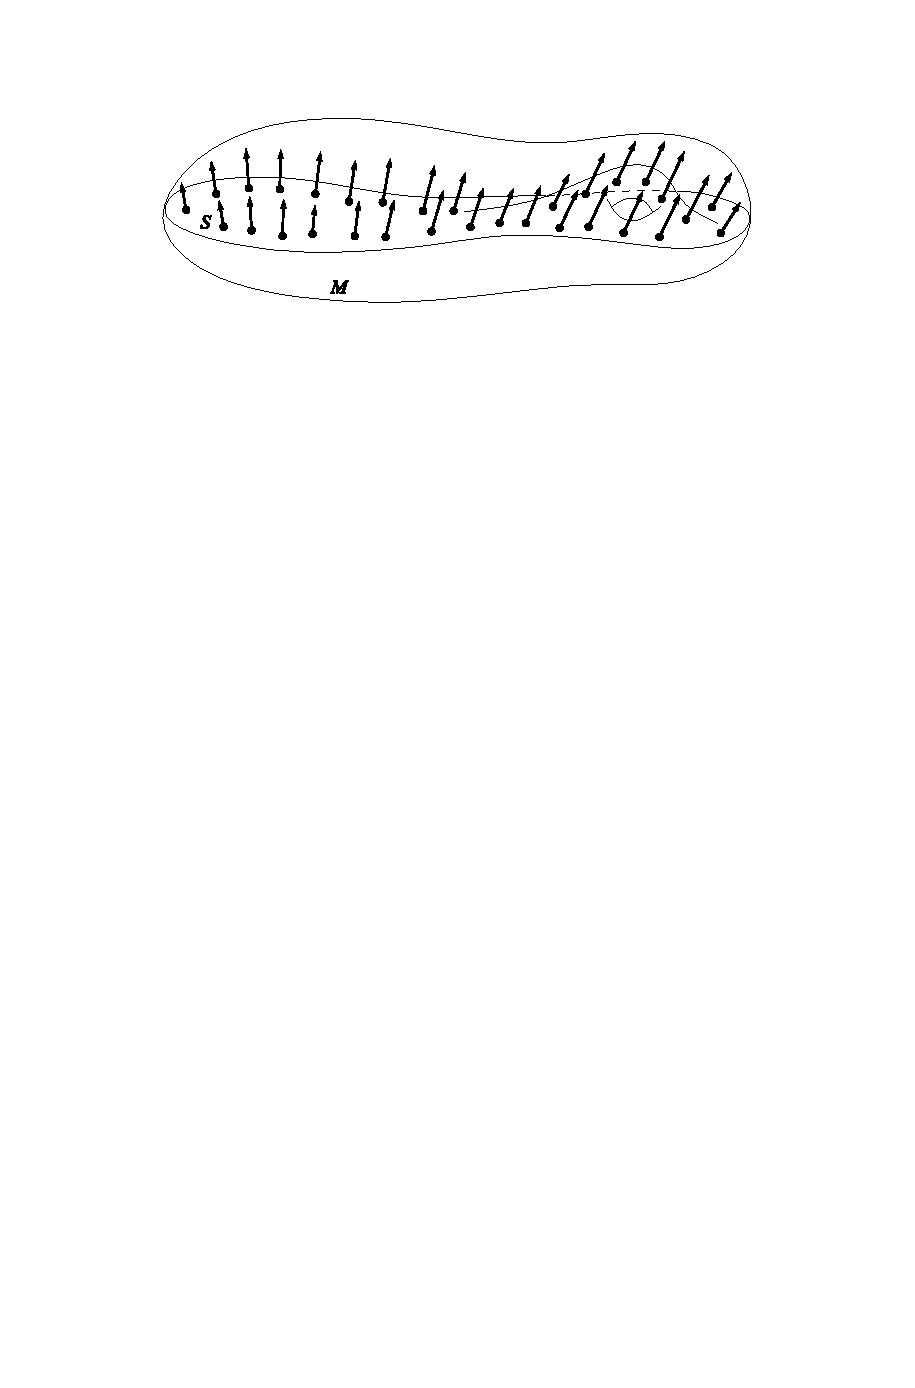
\includegraphics{pictures/vector-field-along}
\caption{A vector field along a submanifold.}
\end{figure}
\begin{proposition}\label{orientation hypersurface}
Suppose $M$ is an oriented smooth n-manifold with or without boundary, $S$ is an immersed hypersurface with or without boundary in $M$, and $N$ is a vector field along $S$ that is nowhere tangent to $S$. Then $S$ has a unique orientation such that for each $p\in S$, $(E_1,\dots,E_{n-1})$ is an oriented basis for $T_pS$ if and only if $(N_p,E_1,\dots,E_{n-1})$ is an oriented basis for $T_pM$. If $\omega$ is an orientation form for $M$, then $\iota^*_S(N\intprod\omega)$ is an orientation form for $S$ with respect to this orientation, where $\iota_S:S\hookrightarrow M$ is inclusion.
\end{proposition}
\begin{remark}
When $n=1$, since $S$ is a $0$-manifold, this proposition should be interpreted as follows: at each point $p\in S$, we assign the orientation $+1$ to $p$ if $N_p$ is an oriented basis for $T_pM$, and $-1$ if $N_p$ is negatively oriented. With this understanding, the proof below goes through in the $n=1$ case without modification.
\end{remark}
\begin{figure}[htbp]
\centering
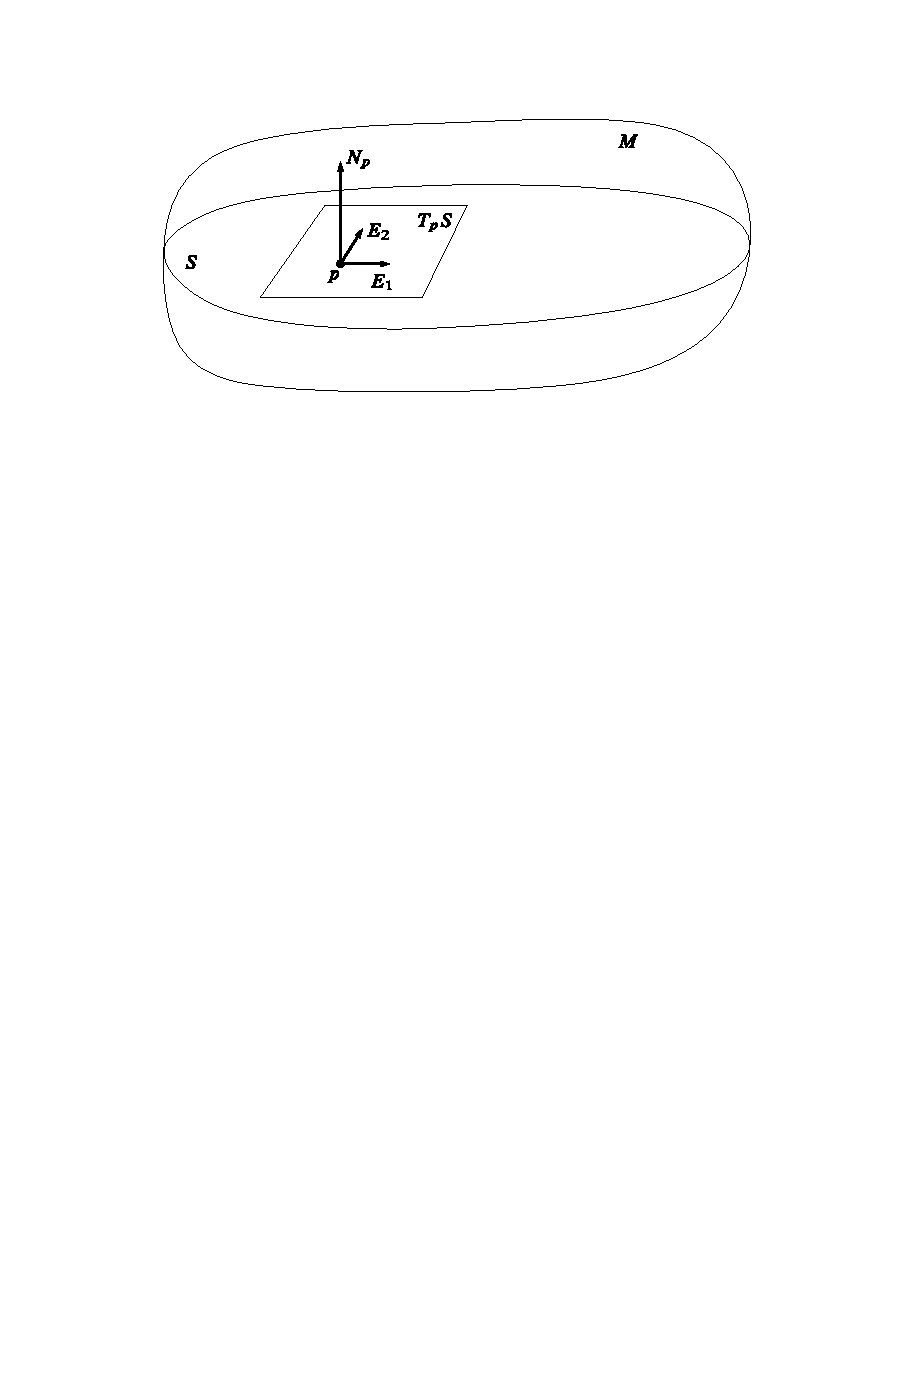
\includegraphics{pictures/orientation-hyper}
\caption{The orientation induced by a nowhere tangent vector field.}
\end{figure}
\begin{proof}
Let $\omega$ be an orientation form for $M$. Then $\sigma=\iota^*_S(N\intprod\omega)$ is an $(n-1)$-form on $S$. (Recall that the pullback 	$\iota_S^*$ is really just restriction to vectors tangent to $S$.) It will follow that $\sigma$ is an orientation form for $S$ if we can show that it never vanishes. Given any basis $(E_1,\dots,E_{n-1})$ for $T_pS$, the fact that $N$ is nowhere tangent to $S$ implies that $(N_p,E_1,\dots,E_{n-1})$ is a basis for $T_pM$. The fact that $N$ is nonvanishing
implies that
\[\sigma_p(E_1,\dots,E_{n-1})=\omega_p(N_p,E_1,\dots,E_{n-1})\neq 0.\]
Since $\sigma_p(E_1,\dots,E_{n-1})>0$ if and only if $\omega_p(N_p,E_1,\dots,E_{n-1})>0$, the orientation determined by $\sigma$ is the one defined in the statement of the proposition.
\end{proof}
\begin{example}
The sphere $S^n$ is a hypersurface in $\R^{n+1}$, to which the vector field $N=x^i\partial/\partial x^i$ is nowhere tangent, so this vector field induces an orientation on $S^n$. This shows that all spheres are orientable. We define the \textbf{standard orientation} of $S^n$ to be the orientation determined by $N$. Unless otherwise specified, we always use this orientation. $($The standard orientation on $S^0$ is the one that assigns the orientation $+1$ to the point $+1$ and $-1$ to $-1\in S^0$.$)$
\end{example}
Not every hypersurface admits a nowhere tangent vector field. However, the following proposition gives a sufficient condition that holds in many cases.
\begin{proposition}
Let $M$ be an oriented smooth manifold, and suppose $S\sub M$ is a regular level set of a smooth function $f:M\to\R$. Then $S$ is orientable.
\end{proposition}
\begin{proof}
Choose any Riemannian metric on $M$, and let $N=\grad f|_S$. The hypotheses imply that $N$ is a nowhere tangent vector field along $S$, so the result follows from Proposition~\ref{orientation hypersurface}.
\end{proof}
\subsubsection{Boundary orientations}
If $M$ is a smooth manifold with boundary, then $\partial M$ is an embedded hypersurface in $M$, and Exercise~\ref{vector field inward} showed that there is always a smooth outward-pointing vector field along $\partial M$. Because an outward-pointing vector field is nowhere tangent to $\partial M$, it determines an orientation on $\partial M$ if $M$ is oriented.
\begin{proposition}[\textbf{Induced Orientation on a Boundary}]
Let $M$ be an oriented smooth $n$-manifold with boundary, $n\geq1$. Then $\partial M$ is orientable, and all outward-pointing vector fields along $\partial M$ determine the same orientation on $\partial M$.
\end{proposition}
\begin{remark}
The orientation on $\partial M$ determined by any outward-pointing vector field is called the \textbf{induced orientation} or the \textbf{Stokes orientation} on $\partial M$.
\end{remark}
\begin{proof}
Let $n=\dim M$, let $\omega$ be an orientation form for $M$, and let $N$ be a smooth
outward-pointing vector field along $\partial M$. The $(n-1)$-form $\iota_{\partial M}^*(N\intprod\omega)$ is an orientation form for $\partial M$ by Proposition~\ref{orientation hypersurface}, so $\partial M$ is orientable.\par
To show that this orientation is independent of the choice of $N$, let $p\in\partial M$ be arbitrary, and let $(x^i)$ be smooth boundary coordinates for $M$ on a neighborhood of $p$. If $N$ and $\widetilde{N}$ are two different outward-pointing vector fields along $\partial M$, Proposition~\ref{inward outward vector iff} shows that the last components $N^n(p)$ and $\widetilde{N}^n(p)$ are both negative. Both $(N_p,\partial/\partial x^1|_p,\dots,\partial/\partial x^n|_p)$ and $(\widetilde{N}_p,\partial/\partial x^1|_p,\dots,\partial/\partial x^n|_p)$ are bases for $T_pM$, and the transition matrix between them has determinant equal to $N^n(p)/\widetilde{N}^n(p)>0$. Thus, both bases determine the same orientation for $T_pM$, so $N$ and $\widetilde{N}$ determine the same orientation for $T_p\partial M$. (When $n=1$, the bases in question are just $N_p$ and $\widetilde{N}_p$, which determine the same orientation because they are both negative multiples of $\partial/\partial x^1|_p$.)
\end{proof}
\begin{example}
This proposition gives a simpler proof that $S^n$ is orientable, because it is the boundary of the closed unit ball. The orientation thus induced on $S^n$ is the standard one.
\end{example}
\begin{example}\label{orientation induce H^n}
Let us determine the induced orientation on $\partial\H^n$ when $\H^n$ itself has the standard orientation inherited from $\R^n$. We can identify $\partial\H^n$ with $\R^{n-1}$ under the correspondence $(x^1,\dots,x^{n-1},0)\leftrightarrow(x^1,\dots,x^{n-1})$. Since the vector field $-\partial/\partial x^n$ is outward-pointing along $\partial\H^n$, the standard coordinate frame for $\R^{n-1}$ is positively oriented for $\partial\H^n$ if and only if $[-\partial/\partial x^n,\partial/\partial x^1,\dots,\partial/\partial x^{n-1}]$ is the standard orientation for $\R^n$. This orientation satisfies
\begin{align*}
[-\partial/\partial x^n,\partial/\partial x^1,\dots,\partial/\partial x^{n-1}]&=-[\partial/\partial x^n,\partial/\partial x^1,\dots,\partial/\partial x^{n-1}]\\
&=(-1)^n[\partial/\partial x^1,\partial/\partial x^2,\dots,\partial/\partial x^{n}].
\end{align*}
Thus, the induced orientation on $\partial\H^n$ is equal to the standard orientation on $\R^{n-1}$ when $n$ is even, but it is opposite to the standard orientation when $n$ is odd. In particular, the standard coordinates on $\partial\H^n\approx\R^{n-1}$ are positively oriented if and only if $n$ is even.
\end{example}
For many purposes, the most useful way of describing submanifolds is by means
of local parametrizations. The next lemma gives a useful criterion for checking
whether a local parametrization of a boundary is orientation-preserving.
\begin{lemma}\label{orientation preserve lem}
Let $M$ be an oriented smooth $n$-manifold with boundary. Suppose $U\sub\R^{n-1}$ is open, $a,b$ are real numbers with $a<b$, and $F:(a,b]\times U\to M$ is a smooth embedding that restricts to an embedding of $\{b\}\times U$ to $\partial M$. Then the parametrization $f:U\to\partial M$ given by $f(x)=F(b,x)$ is orientation-preserving
for $\partial M$ if and only if $F$ is orientation-preserving for $M$.
\end{lemma}
\begin{figure}[htbp]
\centering
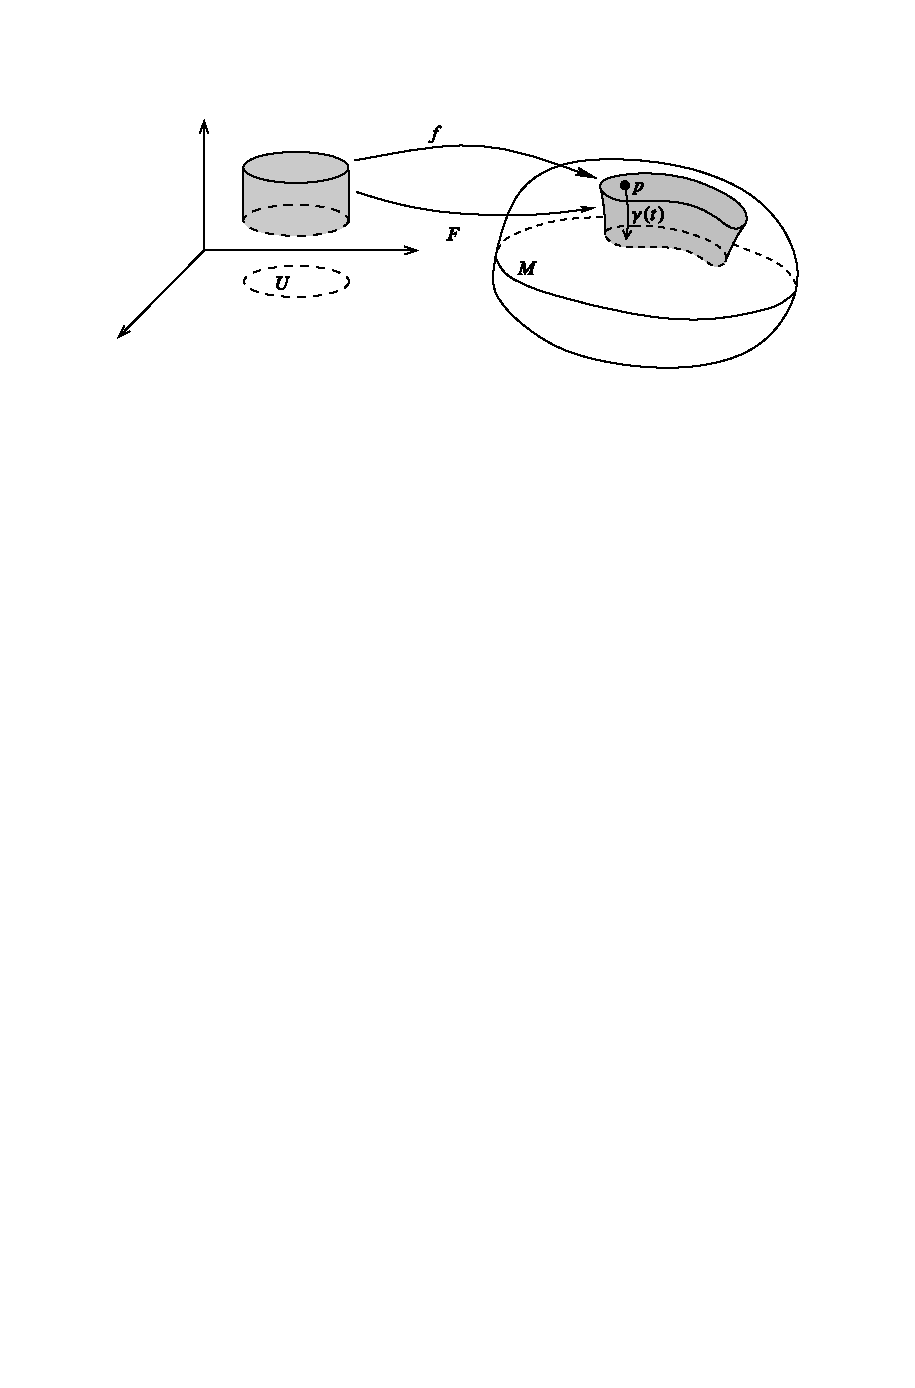
\includegraphics{pictures/boundary-para}
\caption{Orientation criterion for a boundary parametrization.}
\end{figure}
\begin{proof}
Let $x$ be an arbitrary point of $U$, and let $p=f(x)=F(b,x)\in\partial M$. The hypothesis that $F$ is an embedding means that the linear map $dF_{(b,x)}:(T_b\R\oplus T_x\R^{n-1})\to T_pM$ is bijective. Since the restriction of $dF_{(b,x)}$ to $T_x\R^{n-1}$ is equal to $df_x:T_x\R^{n-1}\to T_p\partial M$ which is already injective, it follows that $dF(\partial/\partial s|_{(b,x)})\notin T_p\partial M$ (where $s$ denotes the coordinate on $(a,b]$).\par
Define a smooth curve $\gamma:[0,\eps)\to M$ by
\[\gamma(t)=F(b-t,x).\]
This curve satisfies $\gamma(0)=p$ and $\gamma'(0)=-dF(\partial/\partial s|_{(b,x)})$. It follows that $-dF(\partial/\partial s|_{(b,x)})$ is inward-pointing, and therefore $dF(\partial/\partial s|_{(b,x)})$ is outward-pointing.\par
The definition of the induced orientation yields the following equivalences:
\begin{align*}
F&\text{ is orientation-preserving for $M$}\\
&\iff \text{$\big(dF(\partial/\partial s),dF(\partial/\partial x^1),\dots,dF(\partial/\partial x^{n-1})\big)$ is oriented for $TM$}\\
&\iff \text{$\big(dF(\partial/\partial x^1),\dots,dF(\partial/\partial x^{n-1})\big)$ is oriented for $T\partial M$}\\
&\iff \text{$\big(df(\partial/\partial x^1),\dots,df(\partial/\partial x^{n-1})\big)$ is oriented for $T\partial M$}\\
&\iff\text{$f$ is orientation-preserving for $M$.}
\end{align*}
This proves the claim.
\end{proof}
Here is an illustration of how the lemma can be used.
\begin{figure}[htbp]
\centering
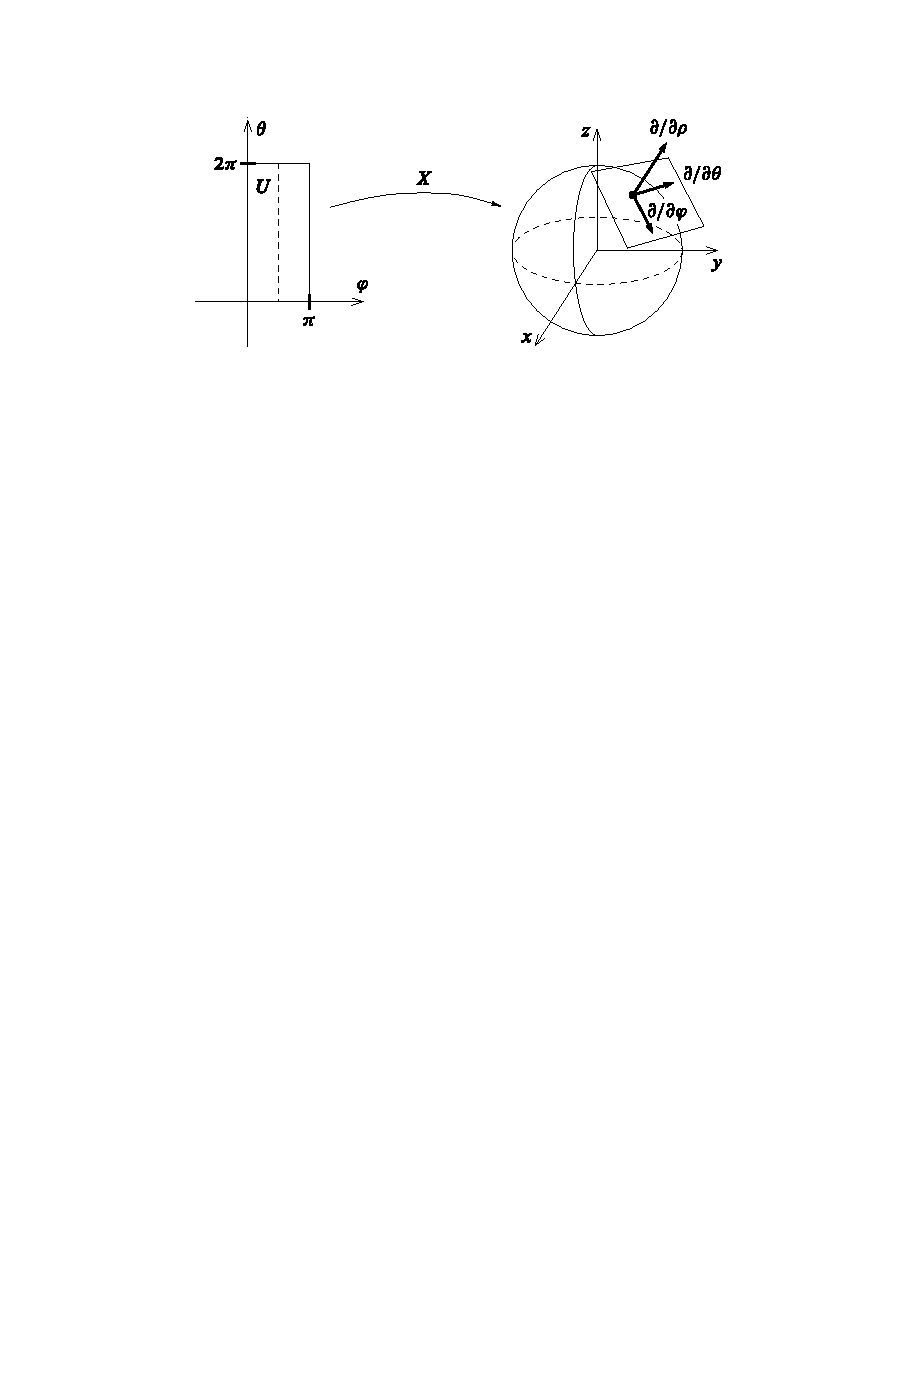
\includegraphics{pictures/spherical-coordinates}
\caption{Parametrizing the sphere via spherical coordinates.}
\end{figure}
\begin{example}\label{orientation para eg}
Spherical coordinates yield a smooth local parametrization of $S^2$ as follows. Let $U$ be the open rectangle $(0,\pi)\times(0,2\pi)\sub\R^2$, and let $X:U\to\R^3$ be the following map:
\[X(\varphi,\theta)=(\sin\varphi\cos\theta,\sin\varphi\sin\theta,\cos\varphi).\]
We can check whether $X$ preserves or reverses orientation by using the fact that it is the restriction of the $3$-dimensional spherical coordinate parametrization $F:(0,1]\times U\to\widebar{B}^3$ defined by
\[F(\rho,\varphi,\theta)=(\rho\sin\varphi\cos\theta,\rho\sin\varphi\sin\theta,\rho\cos\varphi).\]
Because $F(1,\varphi,\theta)=X(\varphi,\theta)$, the hypotheses of Lemma~\ref{orientation preserve lem} are satisfied. By direct computation, the Jacobian determinant of $F$ is $\rho^2\sin\varphi$, which is positive on $(0,1]\times U$. By virtue of Lemma~\ref{orientation preserve lem}, $X$ is orientation-preserving.
\end{example}
\subsection{The Riemannian volume form}
Let $(M,g)$ be an oriented Riemannian manifold of positive dimension. We know from Proposition~\ref{Gram Schmidt Riemannian} that there is a smooth orthonormal frame $(E_1,\dots,E_n)$ in a neighborhood of each point of $M$. By replacing $E_1$ by $-E_1$ if necessary, we can find an oriented orthonormal frame in a neighborhood of each point.
\begin{proposition}\label{Riemannian volume form}
Suppose $(M,g)$ is an oriented Riemannian $n$-manifold with or without boundary, and $n\geq1$. There is a unique smooth orientation form $\omega_g\in\Omega^k(M)$, called the \textbf{Riemannian volume form}, that satisfies
\begin{align}\label{Riemannian volume form-1}
\omega_g(E_1,\dots,E_n)=1
\end{align}
for every local oriented orthonormal frame $(E_i)$ for $M$.
\end{proposition}
\begin{proof}
Suppose first that such a form $\omega_g$ exists. If $(E_1,\dots,E_n)$ is any local oriented orthonormal frame on an open subset $U\sub M$ and $(\eps^1,\dots,\eps^n)$ is the dual coframe, we can write $\omega_g=f\eps^1\wedge\cdots\wedge\eps^n$ on $U$. The condition $(\ref{Riemannian volume form-1})$ then reduces to $f=1$, so
\begin{align}\label{Riemannian volume form-2}
\omega_g=\eps^1\wedge\cdots\wedge\eps^n.
\end{align}
This proves that such a form is uniquely determined.\par
To prove existence, we would like to define $\omega_g$ in a neighborhood of each point
by $(\ref{Riemannian volume form-2})$, so we need to check that this definition is independent of the choice of oriented orthonormal frame. If $(\widetilde{E}_1,\dots,\widetilde{E}_n)$ is another oriented orthonormal frame, with dual coframe $(\widetilde{\eps}^1,\dots,\widetilde{\eps}^n)$, let
\[\widetilde{\omega}=\widetilde{\eps}^1\wedge\dots\wedge\widetilde{\eps}^n.\]
We can write
\[\widetilde{E}_i=A^j_iE_j\]
for some matrix $(A^j_i)$ of smooth functions. The fact that both frames are orthonormal means that $(A^j_i(p))\in\O(n)$ for each $p$, so $\det(A^j_i)=\pm 1$, and the fact that the two frames are consistently oriented forces the positive sign. We compute by Proposition~\ref{alt n tensor linear map}:
\[\omega_g(\widetilde{E}_1,\dots,\widetilde{E}_n)=\det\big(\eps^j(\widetilde{E}_i)\big)=\det(A^j_i)=1=\widetilde{\omega}_g(\widetilde{E}_1,\dots,\widetilde{E}_n).\]
Thus $\omega_g=\widetilde{\omega}_g$, so defining $\omega_g$ in a neighborhood of each point by $(\ref{Riemannian volume form-2})$ with respect to some smooth oriented orthonormal frame yields a global $n$-form. The resulting form is clearly smooth and satisfies $(\ref{Riemannian volume form-1})$ for every oriented orthonormal frame.
\end{proof}
\begin{proposition}
Suppose $(M,g)$ and $(\widetilde{M},\widetilde{g})$ are positive-dimensional Riemannian manifolds with or without boundary, and $F:M\to\widetilde{M}$ is a orientation-preserving local isometry. Then
that $F^*\omega_{\widetilde{g}}=\omega_g$.
\end{proposition}
\begin{proof}
Since $F$ is a orientation-preserving local isometry, it maps a local oriented orthonormal frame to a local oriented orthonormal frame. Then the claim follows immediately.
\end{proof}
Although the expression for the Riemannian volume form with respect to an oriented orthonormal frame is particularly simple, it is also useful to have an expression
for it in coordinates.
\begin{proposition}\label{Riemann volume form formula}
Let $(M,g)$ be an oriented Riemannian $n$-manifold with or without boundary with$n\geq1$. In any oriented smooth coordinates $(x^i)$, the Riemannian volume form has the local coordinate expression
\[\omega_g=\sqrt{G}\, dx^1\wedge\cdots\wedge dx^n,\]
where $G=\det(g_{ij})$ with $g_{ij}$ the components of $g$ in these coordinates.
\end{proposition}
\begin{proof}
Let $(U,(x^i))$ be an oriented smooth chart, and let $p\in M$. In these coordinates, $\omega_g=f\,dx^1\wedge\cdots\wedge dx^n$ for some positive coefficient function $f$. To compute $f$, let $(E_i)$ be any smooth oriented orthonormal frame defined on a neighborhood of $p$, and let $(\eps^i)$ be the dual coframe. If we write the coordinate frame in terms of the orthonormal frame as
\[\frac{\partial}{\partial x^i}=A^j_iE_j,\]
then we can compute
\[f=\omega_g\Big(\frac{\partial}{\partial x^1},\dots,\frac{\partial}{\partial x^n}\Big)=\det\Big(\eps^j\Big(\frac{\partial}{\partial x^i}\Big)\Big)=\det(A^j_i).\]
On the other hand, observe that
\[g_{ij}=\Big\langle\frac{\partial}{\partial x^i},\frac{\partial}{\partial x^j}\Big\rangle_g=\langle A^k_iE_k,A^l_jE_l\rangle_g=A^k_iA^l_j\langle E_k,E_l\rangle_g=\sum_kA^k_iA^k_j.\]
This last expression is the $(i,j)$-entry of the matrix product $A^TA$, where $A=(A^j_i)$. Thus,
\[G:=\det(g_{ij})=\det(A^TA)=(\det A)^2,\]
Since both frames $(\partial/\partial x^i)$ and $(E_i)$ are oriented, $f$ must be positive. So it follows that $f=\sqrt{G}$. 
\end{proof}
\subsubsection{Hypersurfaces in Riemannian manifolds}
Let $(M,g)$ be an oriented Riemannian manifold with or without boundary, and suppose $S\sub M$ is an immersed hypersurface with or without boundary. Any unit normal vector field along $S$ is nowhere tangent to $S$, so it determines an orientation of $S$ by Proposition~\ref{orientation hypersurface}. The next proposition gives a simple formula for the volume form of the induced metric on $S$ with respect to this orientation.
\begin{proposition}\label{Riemann volumn form hyper}
Let $(M,g)$ be an oriented Riemannian manifold with or without boundary, let $S\sub M$ be an immersed hypersurface with or without boundary, and let $\widetilde{g}$ denote the induced metric on $S$. Suppose $N$ is a smooth unit normal vector field along $S$. With respect to the orientation of $S$ determined by $N$, the volume form of $(S,\widetilde{g})$ is given by
\[\omega_{\widetilde{g}}=\iota_S^*(N\intprod\omega_g).\]
\end{proposition}
\begin{proof}
By Proposition~\ref{orientation hypersurface}, the $(n-1)$-form $\iota_S^*(N\intprod\omega_g)$ is an orientation form for $S$. To prove that it is the volume form for the induced Riemannian metric, we need only show that it gives the value $1$ whenever it is applied to an oriented orthonormal frame for $S$. Thus, let $(E_1,\dots,E_{n-1})$ be such a frame. At each point $p\in S$, the basis $(N_p,E_1|_p,\dots,E_{n-1}|_p)$ is orthonormal, and is oriented for $T_pM$ (this is the definition of the orientation determined by $N$). Thus 
\[\iota_S^*(N\intprod\omega_g)(E_1,\dots,E_{n-1})=\omega_g(N,E_1,\dots,E_{n-1})=1,\]
which proves the result.
\end{proof}
The result of Proposition~\ref{Riemann volumn form hyper} takes on particular importance in the case of a Riemannian manifold with boundary, because of the following proposition.
\begin{proposition}
Suppose $M$ is any Riemannian manifold with boundary. There is a unique smooth outward-pointing unit normal vector field $N$ along $\partial M$.
\end{proposition}
\begin{proof}
First, we prove uniqueness. At any point $p\in\partial M$, the subspace $(T_p\partial M)^\bot\sub T_pM$ is $1$-dimensional, so there are exactly two unit vectors at $p$ that are normal to $\partial M$. Since any unit normal vector $N$ is nowhere tangent to $\partial M$, it must have nonzero $x^n$-component in any smooth boundary chart. Thus, exactly one of the two choices of unit normal has negative $x^n$-component, which is equivalent to being outward-pointing.\par
To prove existence, let $f:M\to\R$ be a boundary defining function (Proposition
5.43), and let $N$ be the restriction to $\partial M$ of the unit vector field $-\grad f/|\grad f|_g$. Because $df\neq0$ at points of $\partial M$, $N$ is well-defined and
smooth on $\partial M$. Then $N$ is normal to $\partial M$ by Exercise~\ref{Riemann grad prop}, and outward pointing by Proposition~\ref{inward derivative crit}, because 
\[Nf=\frac{-\langle\grad f,\grad f\rangle_g}{|\grad f|_g}=-|\grad f|_g<0.\]
\end{proof}
The next corollary is immediate.
\begin{corollary}
If $(M,g)$ is an oriented Riemannian manifold with boundary and $\widetilde{g}$ is the induced Riemannian metric on $\partial M$, then the volume form of $\widetilde{g}$ is
\[\omega_{\widetilde{g}}=\iota_{\partial M}^*(N\intprod\omega_g),\]
where $N$ is the outward unit normal vector field along $\partial M$.
\end{corollary}
\subsection{Orientations and covering maps}
Although it is often easy to prove that a given smooth manifold is orientable by constructing an orientation for it, proving that a manifold is not orientable can be much trickier. The theory of covering spaces provides one of the most useful techniques
for doing so. In this part, we explore the close relationship between orientability
and covering maps.\par
Our first result is a simple application of pullback orientations.
\begin{proposition}
If $\pi:E\to M$ is a smooth covering map and $M$ is orientable, then $E$ is also orientable.
\end{proposition}
\begin{proposition}
Because a covering map is a local diffeomorphism, this follows immediately from Proposition~\ref{orientation pull back}.
\end{proposition}
The next theorem is more interesting. If $G$ is a Lie group acting smoothly on a smooth manifold $E$ (on the left, say), we say the action is an \textbf{orientation-preserving action} if for each $g\in G$, the diffeomorphism $x\mapsto g\cdot x$ is orientation-preserving.
\begin{theorem}\label{orientation covering thm}
Suppose $E$ is a connected, oriented, smooth manifold with or without boundary, and $\pi:E\to M$ is a smooth normal covering map. Then $M$ is orientable if and only if the action of $\Aut_\pi(E)$ on $E$ is orientation-preserving.
\end{theorem}
\begin{proof}
Let $\mathcal{O}_E$ denote the given orientation on $E$. First suppose $M$ is orientable, and let $q$ be an arbitrary point in $E$. Because $M$ is connected, it has exactly two orientations, and one of them has the property that $d\pi_q:T_qE\to T_{\pi(q)}M$ is orientation-preserving. Call that orientation $\mathcal{O}_M$. The pullback orientation $\pi^*\mathcal{O}_M$ agrees with the given orientation at $q$, so it must be equal to $\mathcal{O}_E$ by Corollary~\ref{orientation connected}. Suppose $\varphi\in\Aut_\pi(E)$. The fact that $\pi\circ\varphi=\pi$ implies that
\[\varphi^*\mathcal{O}_E=\varphi^*(\pi^*\mathcal{O}_M)=(\pi\circ\varphi)^*\mathcal{O}_M=\pi^*\mathcal{O}_M=\mathcal{O}_E.\]
Thus, $\varphi$ is orientation-preserving.\par
Conversely, suppose the action of $\Aut_\pi(E)$ is orientation-preserving, and let $p\in M$. If $U\sub M$ is any evenly covered neighborhood of $p$, there is a smooth section $\sigma:U\to E$, which induces an orientation $\sigma^*\mathcal{O}_E$ on $U$. Suppose $\sigma_1:U\to E$ is any other smooth local section over $U$. Because $\pi$ is a normal covering, $\Aut_\pi(E)$ acts transitively on each fiber of $\pi$, so there is a covering automorphism $\varphi$ such that $\sigma_1(p)=\varphi(\sigma(p))$. Then $\varphi\circ\sigma$ is a local section of $\pi$ that agrees with $\sigma_1$ at $p$, and thus $\sigma_1=\varphi\circ\sigma$ on all of $U$ by Theorem~\ref{local section unique}. Because $\varphi$ is orientation-preserving, $\sigma_1^*\mathcal{O}_E=\sigma^*\varphi^*\mathcal{O}_E=\sigma^*\mathcal{O}_E$, so the orientations induced by $\sigma$ and $\sigma_1$ are equal. Thus, we can define a global orientation $\mathcal{O}_M$ on $M$ by defining it on each evenly covered open subset to be the pullback orientation induced by any local section; the argument above shows that the orientations so defined agree where they overlap.
\end{proof}
Here are two applications of the preceding theorem.
\begin{example}[\textbf{Orientability of Projective Spaces}]
For $n\geq1$, consider the smooth covering map $q:S^n\to\RP^n$. The only nontrivial covering automorphism of $q$ is the antipodal map $\alpha(x)=-x$. It can be easily shown that $\alpha$ is orientation-preserving if and only if $n$ is odd, so it follows that $\RP^n$ is orientable if and only if $n$ is odd.
\end{example}
\begin{example}[\textbf{The M\"obius Bundle and the M\"obius Band}]
Let $E$ be the total space of the M\"obius bundle $(Example~\ref{Mobius bundle})$. The quotient map $q:\R^2\to E$ used to define $E$ is a smooth normal covering map, and the covering automorphism group is isomorphic to $\Z$, acting on $\R^2$ by 
\[n(x,y)=(x+n,(-1)^ny)\] 
For $n$ odd, the diffeomorphism $(x,y)\mapsto n\cdot (x,y)$ of $\R^2$ pulls back the orientation form $dx\wedge dy$ to $-dx\wedge dy$, so the action of $\Aut_q(E)$ is not orientation-preserving. Thus, Theorem~\ref{orientation covering thm} shows that $E$ is not orientable.\par
For each $r>0$, the image under $q$ of the rectangle $[0,1]\times[-r,r]$ is a M\"obius
band $M_r$. Because $q$ restricts to a smooth covering map from $\R\times[-r,r]$, the
same argument shows that a M\"obius band is not orientable either.
\end{example}
\subsubsection{The orientation covering}
Next we show that every nonorientable smooth manifold $M$ has an orientable two-sheeted
covering manifold. The fiber over a point $p\in M$ will correspond to the two orientations of $T_pM$.\par
In order to handle the orientable and nonorientable cases in a uniform way, it is useful to expand our definition of covering maps slightly, by allowing covering spaces that are not connected. If $N$ and $M$ are topological spaces, let us say that a map $\pi:N\to M$ is a \textbf{generalized covering map} if it satisfies all of the requirements for a covering map except that $N$ might not be connected: this means that $N$ is locally path-connected, $\pi$ is surjective and continuous, and each point $p\in M$ has a neighborhood that is evenly covered by $\pi$. If in addition $N$ and $M$ are smooth manifolds with or without boundary and $\pi$ is a local diffeomorphism, we say it is a \textbf{generalized smooth covering map}.
\begin{lemma}\label{covering restrict}
Suppose $N$ and $M$ are topological spaces and $\pi:N\to M$ is a generalized covering map. If $M$ is connected, then the restriction of $\pi$ to each component of $N$ is a covering map.
\end{lemma}
\begin{proof}
Suppose $W$ is a component of $N$. If $U$ is any open subset of $M$ that is evenly covered by $\pi$, then each component of $\pi^{-1}(U)$ is connected and therefore contained in a single component of $N$. It follows that $(\pi|_W)^{-1}(U)=\pi^{-1}(U)\cap W$ is either the empty set or a nonempty disjoint union of components of $\pi^{-1}(U)$, each of which is mapped homeomorphically onto $U$ by $\pi|_W$. In particular, this means that each point in $\pi(W)$ has a neighborhood that is evenly covered by $\pi|_W$.\par
To complete the proof, we just need to show that $\pi|_W$ is surjective. Because $\pi$
is a local homeomorphism, $\pi(W)$ is an open subset of $M$. On the other hand, if $p\in M-\pi(W)$, and $U$ is a neighborhood of $p$ that is evenly covered by $\pi$, then the discussion in the preceding paragraph shows that $(\pi|_W)^{-1}(U)=\emp$, which implies that $U\sub M-\pi(W)$. Therefore, $\pi(W)$ is closed in $M$. Because $W$ is not empty, $\pi(W)$ is all of $M$.
\end{proof}
Let $M$ be a connected, smooth, positive-dimensional manifold with or without boundary, and let $\widehat{M}$ denote the set of orientations of all tangent spaces to $M$:
\[\widehat{M}=\{(p,\mathcal{O}_p):\text{$p\in M$ and $\mathcal{O}_p$ is an orientation of $T_pM$}\}.\]
Define the projection $\widehat{\pi}:\widehat{M}\to M$ by sending an orientation of $T_pM$ to the point $p$ itself: $\widehat{\pi}(p,\mathcal{O}_p)=p$. Since each tangent space has exactly two orientations, each fiber of this map has cardinality $2$. The map $\widehat{\pi}:\widehat{M}\to M$ is called the \textbf{orientation covering} of $M$.
\begin{proposition}[\textbf{Properties of the Orientation Covering}]\label{orientation cover prop}
Suppose $M$ is a connected, smooth, positive-dimensional manifold with or without boundary, and let $\widehat{\pi}:\widehat{M}\to M$ be its orientation covering. Then $\widehat{M}$ can be given the structure of a smooth, oriented manifold with or without boundary, with the following properties:
\begin{itemize}
\item[(a)] $\widehat{\pi}:\widehat{M}\to M$ is a generalized smooth covering map.
\item[(b)] A connected open subset $U\sub M$ is evenly covered by $\widehat{\pi}$ if and only if $U$ is orientable.
\item[(c)] If $U\sub M$ is an evenly covered open subset, then every orientation of $U$ is the pullback orientation induced by a local section of $\widehat{\pi}$ over $U$.
\end{itemize}
\end{proposition}
\begin{proof}
We first topologize $\widehat{M}$ by defining a basis for it. For each pair $(U,\mathcal{O})$, where $U$ is an open subset of $M$ and $\mathcal{O}$ is an orientation on $U$, define a subset $\widehat{U}_\mathcal{O}\sub\widehat{M}$ as follows:
\[\widehat{U}_\mathcal{O}=\{(p,\mathcal{O}_p)\in\widehat{M}:\text{$p\in U$ and $\mathcal{O}_p$ is the orientation of $T_pM$ determined by $\mathcal{O}$}\}.\]
We will show that the collection of all subsets of the form $\widehat{U}_\mathcal{O}$ is a basis for a topology on $\widehat{M}$.
\begin{itemize}
\item Given an arbitrary point $(p,\mathcal{O}_p)\in\widehat{M}$, let $U$ be an orientable neighborhood of $p$ in $M$, and let $\mathcal{O}$ be an orientation on it. After replacing $\mathcal{O}$ by $-\mathcal{O}$ if necessary, we may assume that the given orientation $\mathcal{O}_p$ is same as the orientation of $T_pM$ determined by $\mathcal{O}$. It follows that $(p,\mathcal{O}_p)\in\widehat{U}_\mathcal{O}$, so the collection of all sets of the form $\widehat{U}_\mathcal{O}$ covers $\widehat{M}$.
\item If $\widehat{U}_\mathcal{O}$ and $\widehat{U}'_{\mathcal{O}'}$ are two such sets and $(p,\mathcal{O}_p)$ is a point in their intersection, then $\mathcal{O}_p$ is the orientation of $T_pM$ determined by both $\mathcal{O}$ and $\mathcal{O}'$. If $V$ is the component of $U\cap U'$ containing $p$, then the restricted orientations $\mathcal{O}|_V$ and $\mathcal{O}'|_V$ agree at $p$ and therefore are identical by Proposition~\ref{orientation connected}, so it follows that $\widehat{U}_\mathcal{O}\cap\widehat{U}'_{\mathcal{O}'}$ contains the basis set $\widehat{V}_{\mathcal{O}|_V}$.
\end{itemize}
Thus, we have defined a topology on $\widehat{M}$.\par
Note that for each orientable open subset $U\sub M$ and each orientation $\mathcal{O}$ of $U$, $\widehat{\pi}$ maps the basis set $\widehat{U}_{\mathcal{O}}$ bijectively onto $U$. Because the orientable open subsets form a basis for the topology of $M$, this implies that $\widehat{\pi}$ restricts to a homeomorphism from $\widehat{U}_\mathcal{O}$ to $U$. In particular, $\widehat{\pi}$ is a local homeomorphism.\par
Next we show that with this topology, $\widehat{\pi}$ is a generalized covering map. Suppose $U\sub M$ is an orientable connected open subset and $\mathcal{O}$ is an orientation for $U$. Then $\widehat{\pi}^{-1}(U)$ is the disjoint union of open subsets $\widehat{U}_{\mathcal{O}}$ and $\widehat{U}_{-\mathcal{O}}$, and $\widehat{\pi}$ restricts to a homeomorphism from each of these sets to $U$. Thus, each such set $U$ is evenly covered, and it follows that $\widehat{\pi}$ is a generalized covering map. By Lemma~\ref{covering restrict}, $\widehat{\pi}$ restricts to an ordinary covering map on each component of $\widehat{M}$, and so Proposition~\ref{covering mani} shows that each such component is a topological $n$-manifold with or without boundary and has a unique smooth structure making $\widehat{\pi}$ into a smooth covering map. These smooth structures combine to give a smooth structure on all of $\widehat{M}$. This completes the proof of (a).\par
Next we give $\widehat{M}$ an orientation. Let $\widehat{p}=(p,\mathcal{O}_p)$ be a point in $\widehat{M}$. By definition, $\mathcal{O}_p$ is an orientation of $T_pM$, so we can give $T_{\widehat{p}}\widehat{M}$ the unique orientation $\widehat{\mathcal{O}}_{\widehat{p}}$ such that $d\widehat{\pi}_{\widehat{p}}:T_{\widehat{p}}\widehat{M}\to T_pM$ is orientation-preserving. This defines a pointwise orientation $\widehat{\mathcal{O}}$ on $\widehat{M}$. On each basis open subset $\widehat{U}_{\mathcal{O}}$, the orientation $\widehat{O}$ agrees
with the pullback orientation induced from $(U,\mathcal{O})$ by (the restriction of) $\widehat{\pi}$, so it is continuous.\par
Next we prove (b). We showed earlier that every orientable connected open subset
of $M$ is evenly covered by $\widehat{\pi}$. Conversely, if $U\sub M$ is any evenly covered open subset, then there is a smooth local section $\sigma:U\to\widehat{M}$ by Proposition~\ref{local section unique}, which pulls $\widehat{O}$ back to an orientation on $U$ by Proposition~\ref{orientation pull back}.\par 
Finally, to prove (c), assume $U\sub M$ is evenly covered and therefore orientable. Given any orientation $\mathcal{O}$ of $U$, define a section $\sigma:U\to M$ by setting $\sigma(p)=(p,\mathcal{O}_p)$. To see that $\sigma$ is continuous, suppose $\widehat{U}'_{\mathcal{O}'}$ is any basis open subset of $\widehat{M}$. Then for each component $V$ of $U\cap U'$, the restricted orientations $\mathcal{O}|_V$ and $\mathcal{O}'|_V$ must either agree or disagree on all of $V$, so $\sigma^{-1}(\widehat{U}'_{\mathcal{O}'})$ is a union of such components and therefore open.
\end{proof}
\begin{theorem}[\textbf{Orientation Covering Theorem}]
Suppose $M$ is a connected smooth manifold with or without boundary, and let $\widehat{\pi}:\widehat{M}\to M$ be its orientation covering.
\begin{itemize}
\item[(a)] If $M$ is orientable, then $\widehat{M}$ has exactly two components, and the restriction of $\widehat{\pi}$ to each component is a diffeomorphism onto $M$.
\item[(b)] If $M$ is nonorientable, then $\widehat{M}$ is connected, and $\widehat{\pi}$ is a two-sheeted smooth covering map.
\end{itemize}
\end{theorem}
\begin{proof}
If $M$ is orientable, then Proposition~\ref{orientation cover prop}(b) shows that $M$ is evenly covered by $\widehat{\pi}$, which means that $\widehat{M}$ has two components, each mapped diffeomorphically onto $M$.\par
Now assume $M$ is nonorientable. We show first that $\widehat{M}$ is connected. Let $W$ be a component of $\widehat{M}$. Lemma~\ref{covering restrict} shows that $\widehat{\pi}|_W$ is a covering map, so its fibers all have the same cardinality. Because the fibers of $\widehat{\pi}$ have cardinality $2$ and $W$ is not empty, the fibers of $\widehat{\pi}|_W$ must have cardinality $1$ or $2$. If the cardinality were $1$, then $\widehat{\pi}|_W$ would be an injective smooth covering map and thus a diffeomorphism, and its inverse would be a smooth section of $\widehat{\pi}$, which would induce an orientation on $M$. Thus, the cardinality must be $2$, which implies that $W=\widehat{M}$. Because $\widehat{M}$ is connected, $\widehat{\pi}$ is a covering map by Lemma~\ref{covering restrict}, and because it is a local diffeomorphism it is a smooth covering map.
\end{proof}
The orientation covering is sometimes called the \textbf{oriented double covering of $\bm{M}$}. There are other ways of constructing it besides the one we have given here, but as the next theorem shows, the specific details of the construction do not matter, because they all yield isomorphic covering manifolds.
\begin{theorem}[\textbf{Characteristic property of the orientation covering}]\label{orientation cover char}
Let $M$ be a connected nonorientable smooth manifold with or without boundary, and let $\widehat{\pi}:\widehat{M}\to M$ be its orientation covering. If $X$ is any oriented smooth manifold with or without boundary, and $F:X\to M$ is any local diffeomorphism, then there exists a unique orientation-preserving local diffeomorphism $\widehat{F}:X\to\widehat{M}$ such that $\widehat{\pi}\circ\widehat{F}=F$:
\[\begin{tikzcd}
&\widehat{M}\ar[d,"\widehat{\pi}"]\\
X\ar[r,swap,"F"]\ar[ru,dashed,"\widehat{F}"]&M
\end{tikzcd}\]
\end{theorem}
\begin{proof}
At each point $p=F(x)\in M$, since $F$ is a local diffeomorphism, we get a unique orientation of $T_pM$, which we denote by $\mathcal{O}_p$. Then we can define
\[\widehat{F}(x)=(F(x),\mathcal{O}_{F(x)}).\]
It is easy to check that $\widehat{\pi}\circ\widehat{F}=F$. Since $\widehat{\pi}$ is also a local diffeomorphism, it follows that $\widehat{F}$ is also a local diffeomorphism. The orientation-preserving statement is clear from the definition.
\end{proof}
\begin{theorem}[\textbf{Uniqueness of the Orientation Covering}]\label{orientation cover unique}
Let $M$ be a nonorientable connected smooth manifold with or without boundary, and let $\widehat{\pi}:\widehat{M}\to M$ be its orientation covering. If $\widetilde{M}$ is an oriented smooth manifold with or without boundary that admits a two-sheeted smooth covering map $\widetilde{\pi}:\widetilde{M}\to M$, then there exists a unique orientation-preserving diffeomorphism $\varphi:\widetilde{M}\to\widehat{M}$ such that $\widehat{\pi}\circ\varphi=\widetilde{\pi}$.
\end{theorem}
By invoking a little more covering space theory, we obtain the following sufficient
topological condition for orientability. 
\begin{theorem}
Let $M$ be a connected smooth manifold with or without boundary, and suppose the fundamental group of $M$ has no subgroup of index $2$. Then $M$ is orientable. In particular, if $M$ is simply connected then it is orientable.
\end{theorem}
\begin{proof}
Suppose $M$ is not orientable, and let $\widehat{\pi}:\widehat{M}\to M$ be its orientation covering, which is an honest covering map in this case. Choose any point $q\in\widehat{M}$, and let $p=\widehat{\pi}(q)\in M$. Let $\alpha:\widehat{M}\to\widehat{M}$ be the map that interchanges the two points in each fiber of $\widehat{\pi}$. To prove that $\alpha$ is smooth, suppose $U\sub M$ is any evenly covered open subset and $U_0,U_1\sub\widehat{M}$ are the two components of $\widehat{\pi}^{-1}(U)$. Since $\widehat{\pi}$ restricts to a diffeomorphism from each component onto $U$, we can write $\alpha|_{U_0}=(\widehat{\pi}|_{U_1})^{-1}\circ(\widehat{\pi}|_{U_0})$, which is smooth. Similarly, $\alpha|_{U_1}$ is also smooth. Since the collection of all such sets $U_0,U_1$ is an open covering of $\widehat{M}$, it follows that $\alpha$ is smooth, and it is a covering automorphism because it satisfies $\widehat{\pi}\circ\alpha=\widehat{\pi}$. In fact, since a covering automorphism is determined by what it does to one point, $\alpha$ is the unique nontrivial element of the automorphism group $\Aut_{\widehat{\pi}}(\widehat{M})$, which is therefore
equal to the two-element group $\{\mathrm{id}_{\widehat{M}},\alpha\}$. Because the automorphism group acts transitively on fibers, $\widehat{\pi}$ is a normal covering map. A fundamental result in the theory of covering spaces is that
\[\Aut_{\widehat{\pi}}(\widehat{M})\cong\frac{\pi_1(M,p)}{\widehat{\pi}^*\big(\pi_1(\widehat{M},q)\big)}.\]
Therefore, $\pi_1(M,p)$ has an index $2$ subgroup.
\end{proof}
\subsection{Exercise}
\begin{exercise}
Suppose$ M$ is a smooth manifold that is the union of two orientable open submanifolds with connected intersection. Show that $M$ is orientable.
\end{exercise}
\begin{proof}
Use Proposition~\ref{orientation connected}.
\end{proof}
\begin{exercise}
Suppose $M$ and $N$ are oriented smooth manifolds with or without boundary, and $F:M\to N$ is a local diffeomorphism. Show that if $M$ is connected, then $F$ is either orientation-preserving or orientation-reversing.
\end{exercise}
\begin{exercise}
Suppose $n\geq1$, and let $\alpha:S^n\to S^n$ be the antipodal map: $\alpha(x)=-x$. Show that $\alpha$ is orientation-preserving if and only if $n$ is odd.
\end{exercise}
\begin{proof}
Consider the orientation form on $\widebar{B}^{n+1}$:
\[\omega=dx^1\wedge\cdots\wedge dx^{n+1}.\]
The induced orientation on $S^n$ is then given by
\[\omega_{S^n}=\iota^*(N\intprod\omega),\]
where $N=x^i\partial/\partial x^i$. Let $F:\widebar{B}^{n+1}\to\widebar{B}^{n+1}$ be the map $F(x)=-x$, then $F_*\omega=(-1)^{n+1}\omega$. Since the map $\alpha$ preserves that vector field $N$, and the orientation of $S^n$ is induced by $N$, we conclude that $\alpha$ is orientation-preserving if and only if $F$ is orientation-preserving.
\end{proof}
\begin{exercise}\label{orientation flow}
Let $\theta$ be a smooth flow on an oriented smooth manifold with or without boundary. Show that for each $t\in\R$, $\theta_t$ is orientation-preserving wherever it is defined.
\end{exercise}
\begin{proof}
The map $\theta:\R\to\Diff(M)$ is a smooth group homomorphism, and hence its image is connected. Since $\theta_0=\mathrm{id}_M$, this curve lies in the orientation preserving component of $\Diff(M)$.
\end{proof}
\begin{exercise}\label{orentaton TM and T^*M}
Let $M$ be a smooth manifold with or without boundary. Show that the total
spaces of $TM$ and $T^*M$ are orientable.
\end{exercise}
\begin{proof}
We prove for $TM$. By Proposition~\ref{tangent bundle struct}, the transition map between charts $(U,\varphi)$ and $(V,\psi)$ of $M$ is
\[\widetilde{\psi}\circ\widetilde{\varphi}^{-1}(x^1,\dots,x^n,v^1,\dots,v^n)=(\widetilde{x}^1(x),\dots,\widetilde{x}^n(x),v^i\frac{\partial\widetilde{x}^1}{\partial x^i}(x),\dots,v^i\frac{\partial\widetilde{x}^n}{\partial x^i}(x)).\]
The Jacobian matrix of this map is
\[\partial(\widetilde{\psi}\circ\widetilde{\varphi}^{-1})(x,v)=\begin{pmatrix}
\dfrac{\partial\widetilde{x}^j}{\partial x^i}(x)&0\\[8pt]
*&\dfrac{\partial\widetilde{x}^j}{\partial x^i}(x)
\end{pmatrix}.\]
Thus \[\det\partial(\widetilde{\psi}\circ\widetilde{\varphi}^{-1})=\big(\det\partial(\psi\circ\varphi^{-1})\big)^2,\]
which, by Proposition~\ref{orientation by atlas}, implies $TM$ is orientable.
\end{proof}
\begin{exercise}
Suppose $M$ is an oriented Riemannian manifold with or without boundary, and $S\sub M$ is an oriented smooth hypersurface with or without boundary. Show that there is a unique smooth unit normal vector field along $S$ that determines the given orientation of $S$.
\end{exercise}
\begin{exercise}
Suppose $M$ is an orientable Riemannian manifold, and $S\sub M$ is an immersed or embedded submanifold with or without boundary. Prove the following statements.
\begin{itemize}
\item[(a)] If $S$ has trivial normal bundle, then $S$ is orientable.
\item[(b)] If $S$ is an orientable hypersurface, then $S$ has trivial normal bundle.
\end{itemize}
\end{exercise}
\begin{proof}
Let $S$ has codimension $k$. If $S$ has trivial normal bundle, then there is an diffeomorphism $NS\to S\times\R^k$. Thus we have global frames $(\sigma_1,\dots,\sigma_k)$ of $NS$. By Proposition~\ref{local frame completion}, at each point $p$ we can find local frames $(\sigma_{k+1},\dots,\sigma_{n})$ such that $(\sigma_1,\dots,\sigma_n)$ is an oriented frame for $T_pM$. Thus $S$ is orientable.\par
If $S$ is an orientable hypersurface, then there is a unit normal vector field along $S$. Since this is a global frame for $NS$, we get a global trivialization for $NS$.
\end{proof}
\begin{exercise}
Show that every orientation-reversing diffeomorphism of $\R$ has a fixed
point.
\end{exercise}
\begin{exercise}
Let $M$ be a connected smooth $1$-manifold. Show that $M$ is diffeomorphic to either $\R$ or $S^1$, as follows:
\begin{itemize}
\item[(a)] First, do the case in which $M$ is orientable by showing that $M$ admits a nonvanishing smooth vector field.
\item[(b)] Now let $M$ be arbitrary, and prove that $M$ is orientable by showing that its universal covering manifold is diffeomorphic to $\R$.
\end{itemize}
Conclude that the smooth structures on both $\R$ and $S^1$ are unique up to
diffeomorphism.
\end{exercise}
\begin{proof}
The only $1$-manifolds are $\R$ and $S^1$, thus orientable.
\end{proof}
\begin{exercise}
Show that every connected smooth $1$-manifold with nonempty boundary is diffeomorphic to either $[0,\infty)$ or $[0,1]$.
\end{exercise}
\begin{exercise}
Let $M$ be a nonorientable embedded hypersurface in $\R^n$, and let $NM$ be
its normal bundle with projection $\pi_{NM}:NM\to M$. Show that the set
\[W=\{(x,v)\in NM:|v|=1\}\]
is an embedded submanifold of $NM$, and the restriction of $\pi_{NM}$ to $W$ is a smooth covering map isomorphic to the orientation covering of $M$.
\end{exercise}
\begin{proof}
We can show that $W$ is a orientable manifold, and the map $\pi_{NM}:W\to M$ is a $2$-sheet covering. Thus there is a diffeomorphism from $W$ to $\widehat{M}$ by Theorem~\ref{orientation cover unique}.
\end{proof}
\begin{exercise}
Let $E$ be the total space of the M\"obius bundle as in Example~\ref{Mobius bundle}. Show that the orientation covering of $E$ is diffeomorphic to the cylinder $S^1\times\R$.
\end{exercise}
\begin{proof}
Let $S^1\times\R$ be embedded into $\R^3$, we can apply the antipodal map $\alpha$ on it to obtain $E$. This gives a $2$-sheet cover of $E$, and is the orientation covering by Theorem~\ref{orientation cover unique}.
\end{proof}
\section{Integration on manifolds}
\subsection{Integration of differential forms}
In this part we will apply the integration theory on manifolds. In particular, we need the Lebesgue integration in $\R^n$. Let $D\sub\R^n$ be a measurable set, and let $\omega$ be a continuous $n$-form on $\widebar{D}$. Any such form can be written as $\omega=f\,dx^1\wedge\cdots\wedge dx^n$ for some continuous function $f:\widebar{D}\to\R$. We define the \textbf{integral of $\bm{\omega}$ over $\bm{D}$} to be
\[\int_D\omega=\int_Df\,dV.\]
This can be written more suggestively as
\[\int_Df\,dx^1\wedge\cdots\wedge dx^n=\int_Df\,dx^1\cdots dx^n.\]
Somewhat more generally, let $U$ be an open subset of $\R^n$ or $\H^n$, and suppose $\omega$ is a compactly supported $n$-form on $U$. We define
\[\int_U\omega=\int_D\omega,\]
where $D\sub\R^n$ or $\H^n$ is any measurable set containing $\supp(\omega)$, and $\omega$ is extended to be zero on the complement of its support. It is easy to check that this definition does not depend on what domain $D$ is chosen.\par
Like the definition of the integral of a $1$-form over an interval, our definition of the integral of an $n$-form might look like a trick of notation. The next proposition shows why it is natural.
\begin{proposition}\label{int R^n pull back}
Suppose $U$, $V$ are open subsets of $\R^n$ or $\H^n$, and $G:U\to V$ is an orientation-preserving or orientation-reversing diffeomorphism. If $\omega$ is a compactly supported $n$-form on $V$, then
\[\int_V\omega=\pm\int_UG^*\omega.\]
with the positive sign if $G$ is orientation-preserving, and the negative sign otherwise.
\end{proposition}
\begin{figure}[htbp]
\centering
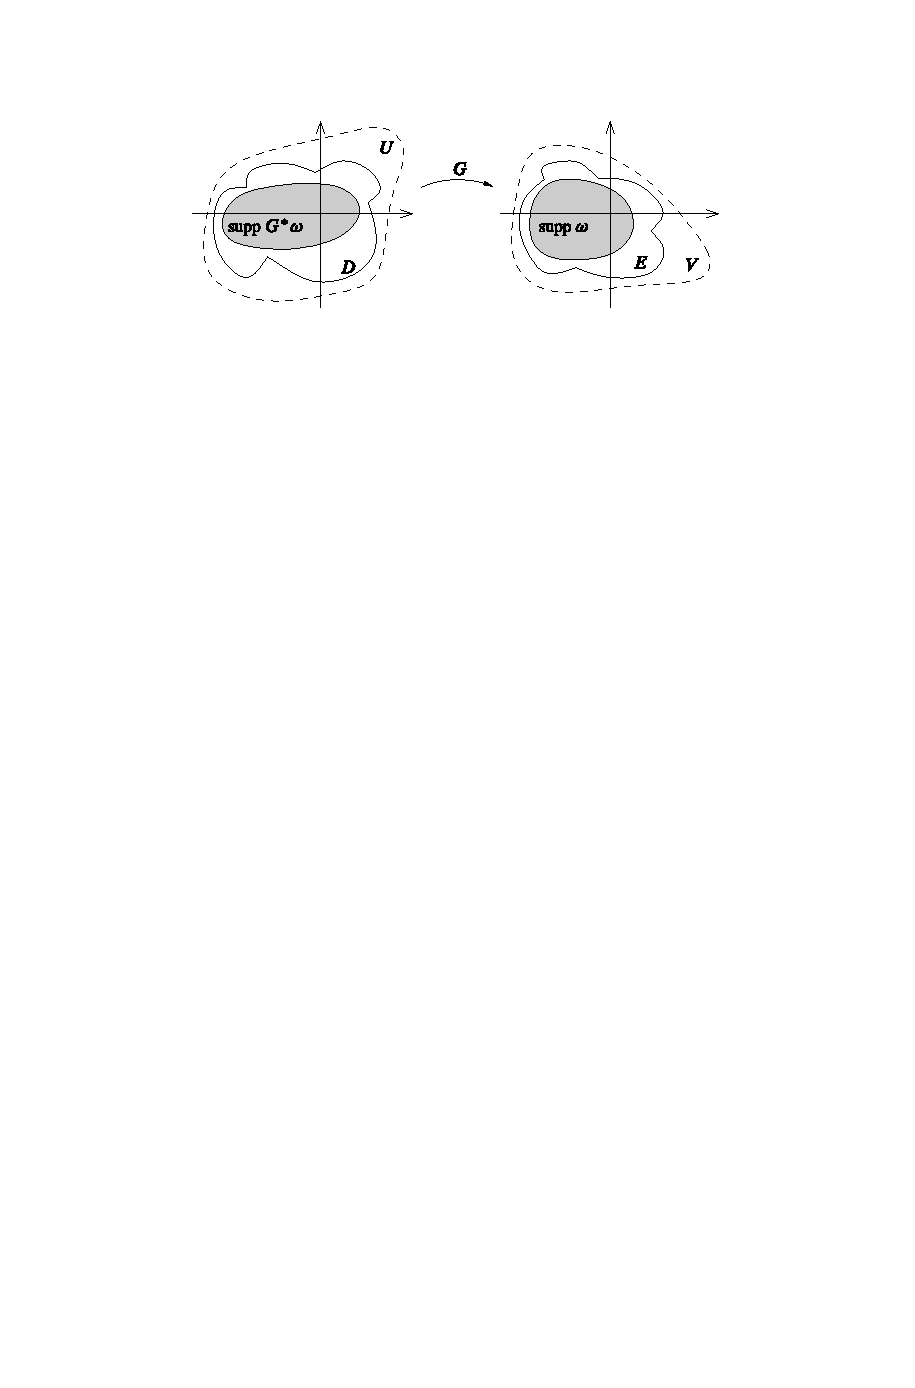
\includegraphics{pictures/int-form-Rn}
\caption{Diffeomorphism invariance of the integral of a form on an open subset.}
\end{figure}
\begin{proof}
Let us use $(y^1,\dots,y^n)$ to denote standard coordinates on $V$, and $(x^1,\dots,x^n)$ to denote those on $U$. Suppose first that $G$ is orientation-preserving. With $\omega=f\,dy^1\wedge\cdots\wedge dy^n$, the change of variables formula together with formula $(\ref{pull back n form-1})$ for pullbacks of $n$-forms yields
\begin{align*}
\int_V\omega&=\int_Vf\,dV=\int_U(f\circ G)|\det\partial G|\,dV=\int_U(f\circ G)(\det\partial G)\,dV\\
&=\int_U(f\circ G)(\det \partial G)\,dx^1\wedge\cdots\wedge dx^n=\int_UG^*\omega.
\end{align*}
If $G$ is orientation-reversing, the same computation holds except that a negative sign is introduced when the absolute value signs are removed.
\end{proof}
\subsubsection{Integration on manifolds}
Let $M$ be an oriented smooth nmanifold with or without boundary, and let $\omega$ be an $n$-form on $M$. Suppose first that $\omega$ is compactly supported in the domain of a single smooth chart $(U,\varphi)$ that is either positively or negatively oriented. We define the integral of $\omega$ over $M$ to be
\begin{align}\label{int mani def-1}
\int_M\omega=\pm\int_{\varphi(U)}\varphi_*\omega,
\end{align}
\begin{figure}[htbp]
\centering
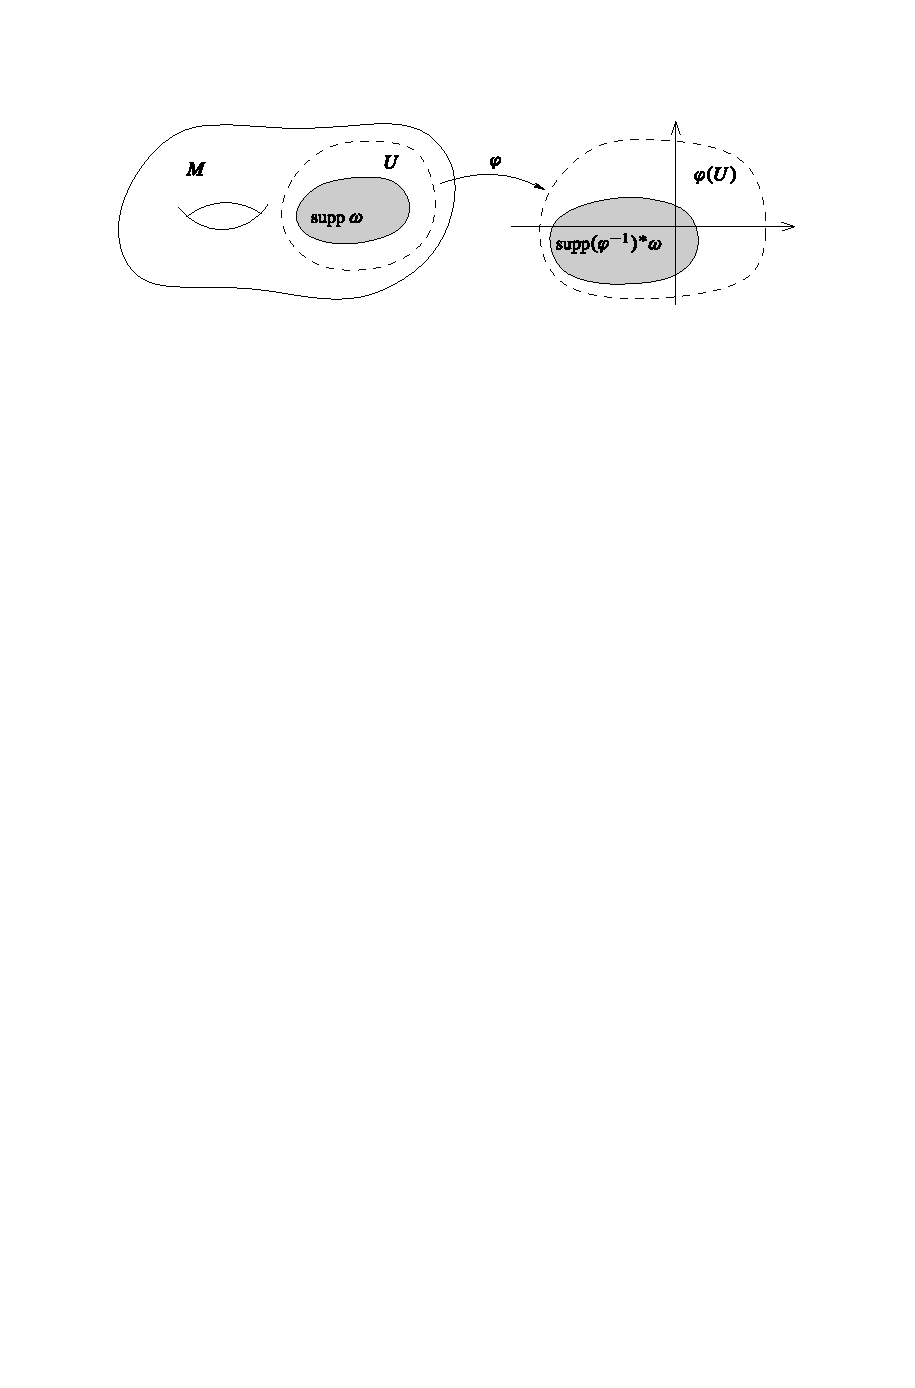
\includegraphics{pictures/int-form-onechart}
\caption{The integral of a form over a manifold.}
\end{figure}
with the positive sign for a positively oriented chart, and the negative sign otherwise. Since $\varphi_*\omega$ is a compactly supported $n$-form on the open subset $\varphi(U)\sub\R^n$ or $\H^n$, its integral is defined as discussed above.
\begin{proposition}\label{inte form one chart}
With $\omega$ as above, $\int_M\omega$ does not depend on the choice of smooth chart whose domain contains $\supp(\omega)$.
\end{proposition}
\begin{figure}[htbp]
\centering
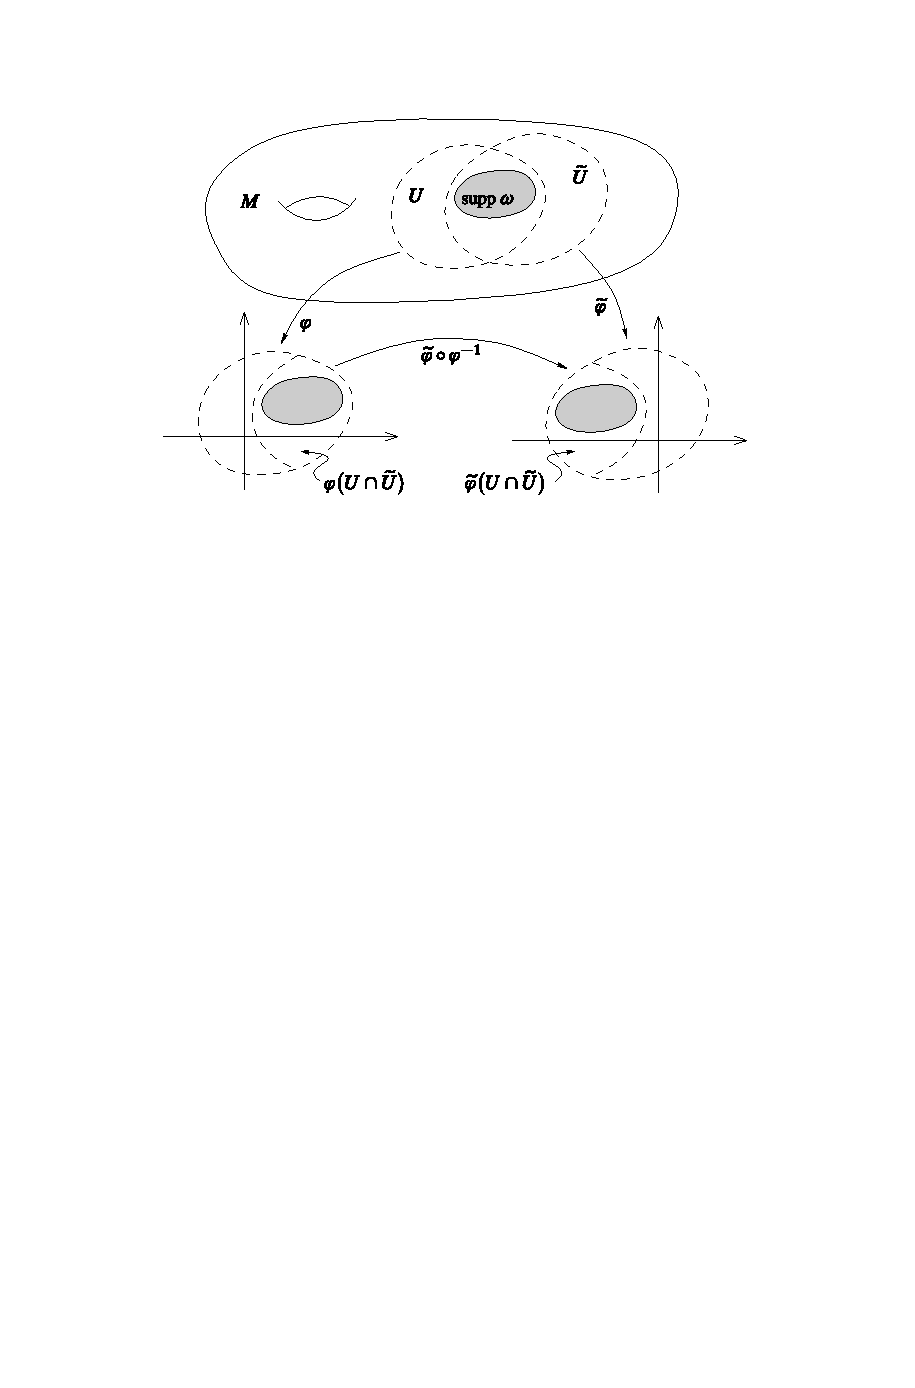
\includegraphics{pictures/int-form-coordinate}
\caption{Coordinate independence of the integral.}
\end{figure}
\begin{proof}
Suppose $(U,\varphi)$ and $(\widetilde{U},\widetilde{\varphi})$ are two smooth charts such that $\supp(\omega)\sub U\cap\widetilde{U}$. If both charts are positively oriented or both are negatively oriented, then $\widetilde{\varphi}\circ\varphi^{-1}$ is an orientation-preserving diffeomorphism from $\varphi(U\cap\widetilde{U})$ to $\widetilde{\varphi}(U\cap\widetilde{U})$, so Proposition~\ref{int R^n pull back} implies that
\begin{align*}
\int_{\widetilde{\varphi}(\widetilde{U})}\widetilde{\varphi}_*\omega&=\int_{\widetilde{\varphi}(U\cap\widetilde{U})}\widetilde{\varphi}_*\omega=\int_{\varphi(U\cap\widetilde{U})}(\widetilde{\varphi}\circ\varphi^{-1})^*\widetilde{\varphi}_*\omega\\
&=\int_{\varphi(U\cap\widetilde{U})}(\varphi^{-1})^*\circ\widetilde{\varphi}^*\circ\widetilde{\varphi}_*\omega=\int_{\varphi(U)}\varphi_*\omega.
\end{align*}
If the charts are oppositely oriented, then the two definitions given by $(\ref{int mani def-1})$ have opposite signs, but this is compensated by the fact that $\widetilde{\varphi}\circ\varphi^{-1}$ is orientationreversing, so Proposition~\ref{int R^n pull back} introduces an extra negative sign into the computation above. In either case, the two definitions of $\int_M\omega$ agree.
\end{proof}
To integrate over an entire manifold, we combine this definition with a partition of unity. Suppose $M$ is an oriented smooth $n$-manifold with or without boundary, and $\omega$ is a compactly supported $n$-form on $M$. Let $\{U_i\}$ be a finite open cover of $\supp(\omega)$ by domains of positively or negatively oriented smooth charts, and let $\{\psi_i\}$ be a subordinate smooth partition of unity. Define the integral of $\omega$ over $M$ to be
\begin{align}\label{int mani def-2}
\int_M\omega=\sum_i\int_{U_i}\psi_i\omega.
\end{align}
(The reason we allow for negatively oriented charts is that it may not be possible to find positively oriented boundary charts on a $1$-manifold with boundary, as noted in the proof of Proposition~\ref{orientation by atlas}.) Since for each $i$, the $n$-form $\psi_i\omega$ is compactly supported in $U_i$, each of the terms in this sum is well defined according to our discussion above. To show that the integral is well defined, we need only examine the dependence on the open cover and the partition of unity.
\begin{proposition}
The definition of $\int_M\omega$ given above does not depend on the choice of open cover or partition of unity.
\end{proposition}
\begin{proof}
Suppose $\{\widetilde{U}_j\}$ is another finite open cover of $\supp(\omega)$ by domains of positively or negatively oriented smooth charts, and $\{\widetilde{\psi}_j\}$ is a subordinate smooth partition of unity. For each $i$, we compute
\[\int_M\psi_i\omega=\int_M\Big(\sum_j\widetilde{\psi}_j\Big)\psi_i\omega=\sum_j\int_M\widetilde{\psi}_j\psi_i\omega.\]
Summing over $i$, we obtain
\[\sum_i\int_M\psi_i\omega=\sum_{i,j}\int_M\widetilde{\psi}_j\psi_i\omega.\]
Observe that each term in this last sum is the integral of a form that is compactly supported in a single smooth chart (e.g., in $U_i$ ), so by Proposition~\ref{inte form one chart} each term is well defined, regardless of which coordinate map we use to compute it. The same argument, starting with $\int_M\widetilde{\psi}_j\omega$, shows that
\[\sum_j\int_M\widetilde{\psi}_j\omega=\sum_{ij}\widetilde{\psi}_j\psi_i\omega.\]
Thus, both definitions yield the same value for $\int_M\omega$.
\end{proof}
As usual, we have a special definition in the zero-dimensional case. The integral of a compactly supported $0$-form (i.e., a real-valued function) $f$ over an oriented
$0$-manifold $M$ is defined to be the sum
\[\int_Mf=\sum_{p\in M}\pm f(p).\]
where we take the positive sign at points where the orientation is positive and the
negative sign at points where it is negative. The assumption that $f$ is compactly
supported implies that there are only finitely many nonzero terms in this sum.\par
If $S\sub M$ is an oriented immersed $k$-dimensional submanifold (with or without
boundary), and $\omega$ is a $k$-form on $M$ whose restriction to $S$ is compactly supported, we interpret $\int_S\omega$ to mean $\int_S\iota_S^*\omega$, where $\iota_S:S\hookrightarrow M$ is inclusion. In particular, if $M$ is a compact, oriented, smooth $n$-manifold with boundary and $\omega$ is an $(n-1)$-form on $M$, we can interpret $\int_{\partial M}\omega$ unambiguously as the integral of $\iota_{\partial M}^*\omega$ over $\partial M$, where $\partial M$ is always understood to have the induced orientation.
\begin{remark}
It is worth remarking that it is possible to extend the definition of the integral to some noncompactly supported forms, and such integrals are important in many
applications. However, in such cases the resulting multiple integrals are improper, so one must pay close attention to convergence issues. For the purposes we have in
mind, the cases we have described here are quite sufficient.
\end{remark}
\begin{proposition}[\textbf{Properties of Integrals of Forms}]\label{int form prop}
Suppose $M$ and $N$ are nonempty oriented smooth $n$-manifolds with or without boundary, and $\omega,\eta$ are compactly supported $n$-forms on $M$.
\begin{itemize}
\item[(a)] Linearity: If $a,b\in\R$, then
\[\int_M(a\omega+b\eta)=a\int_M\omega+b\int_M\eta.\]
\item[(b)] Orientation reversal: If $-M$ denotes $M$ with the opposite orientation,
then
\[\int_{-M}\omega=-\int_M\omega.\]
\item[(c)] Positivity: If $\omega$ is a positively oriented orientation form, then $\int_M\omega>0$.
\item[(d)] Diffeomorphism invariance: If $F:M\to N$ is an orientation-preserving
or orientation-reversing diffeomorphism, then
\[\int_MF^*\omega=\begin{cases}
\quad\displaystyle{\int_{N}\omega}&\text{if $F$ is orientation-preserving,}\vspace{1ex}\\
-\displaystyle{\int_{N}\omega}&\text{if $F$ is orientation-reversing.}
\end{cases}\]
\end{itemize}
\end{proposition}
\begin{proof}
Suppose $\omega$ is a positively oriented orientation form for $M$. This means that if $(U,\varphi)$ is a positively oriented smooth chart, then $\varphi_*\omega$ is a positive function times $dx^1\wedge\cdots\wedge dx^n$, and for a negatively oriented chart it is a negative function times the same form. Therefore, each term in the sum defining $\int_M\omega$ is nonnegative, with at least one strictly positive term, thus proving (c).\par
To prove (d), it suffices to assume that $\omega$ is compactly supported in a single positively or negatively oriented smooth chart, because any compactly supported $n$-form on $N$ can be written as a finite sum of such forms by means of a partition of unity. Thus, suppose $(U,\varphi)$ is a positively oriented smooth chart on $N$ whose domain contains the support of $\omega$. When $F$ is orientation-preserving, it is easy to check that $(F^{-1}(U),\varphi\circ F)$ is an oriented smooth chart on $M$ whose domain contains the support of $F^*\omega$, and the result then follows immediately from Proposition~\ref{inte form one chart}. The cases in which the chart is negatively oriented or $F$ is orientation-reversing then follow from this result together with (b).
\end{proof}
Although the definition of the integral of a form based on partitions of unity is very convenient for theoretical purposes, it is useless for doing actual computations. It is generally quite difficult to write down a smooth partition of unity explicitly, and even when one can be written down, one would have to be exceptionally lucky to be able to compute the resulting integrals.\par
For computational purposes, it is much more convenient to \textit{chop up} the manifold into a finite number of pieces whose boundaries are sets of measure zero, and
compute the integral on each piece separately by means of local parametrizations. One way to do this is described below.
\begin{proposition}[\textbf{Integration Over Parametrizations}]\label{int mani para}
Let $M$ be an oriented smooth $n$-manifold with or without boundary, and $\omega$ be a compactly supported $n$-form on $M$. Suppose that $D_1,\dots,D_k$ are open sets in $\R^n$, and for $1\leq i\leq k$, we are given smooth maps $F_i:D_i\to M$ satisfying
\begin{itemize}
\item[(\rmnum{1})] $F_i$ restricts to an orientation-preserving diffeomorphism from $D_i$ onto an open subset $W_i\sub M$.
\item[(\rmnum{2})] $D_i\cap D_j=\emp$ whenever $i\neq j$.
\item[(\rmnum{3})] $\partial D_i$ has Lebesgue measure zero for each $i$.
\item[(\rmnum{4})] $\supp(\omega)\sub\bigcup_{i=1}^{k}\widebar{W}_i$.
\end{itemize}
Then
\begin{align}\label{inte mani para-1}
\int_M\omega=\sum_{i=1}^{k}\int_{D_i}F_i^*\omega.
\end{align}
\end{proposition}
\begin{proof}
As in the preceding proof, it suffices to assume that $\omega$ is supported in the domain of a single oriented smooth chart $(U,\varphi)$. In fact, by restricting to sufficiently nice charts, we may assume that $U$ is precompact, $Y=\varphi(U)$ is open in $\R^n$ or $\H^n$, and $\varphi$ extends to a diffeomorphism from $\widebar{U}$ to $\widebar{Y}$.\par
For each $i$, define open subsets $A_i\sub D_i,B_i\sub W_i$, and $C_i\sub Y$ by
\[A_i=F_i^{-1}(U\cap W_i),\quad B_i=U\cap W_i=F_i(A_i),\quad C_i=\varphi(B_i)\varphi\circ F_i(A_i).\]
\begin{figure}[htbp]
\centering
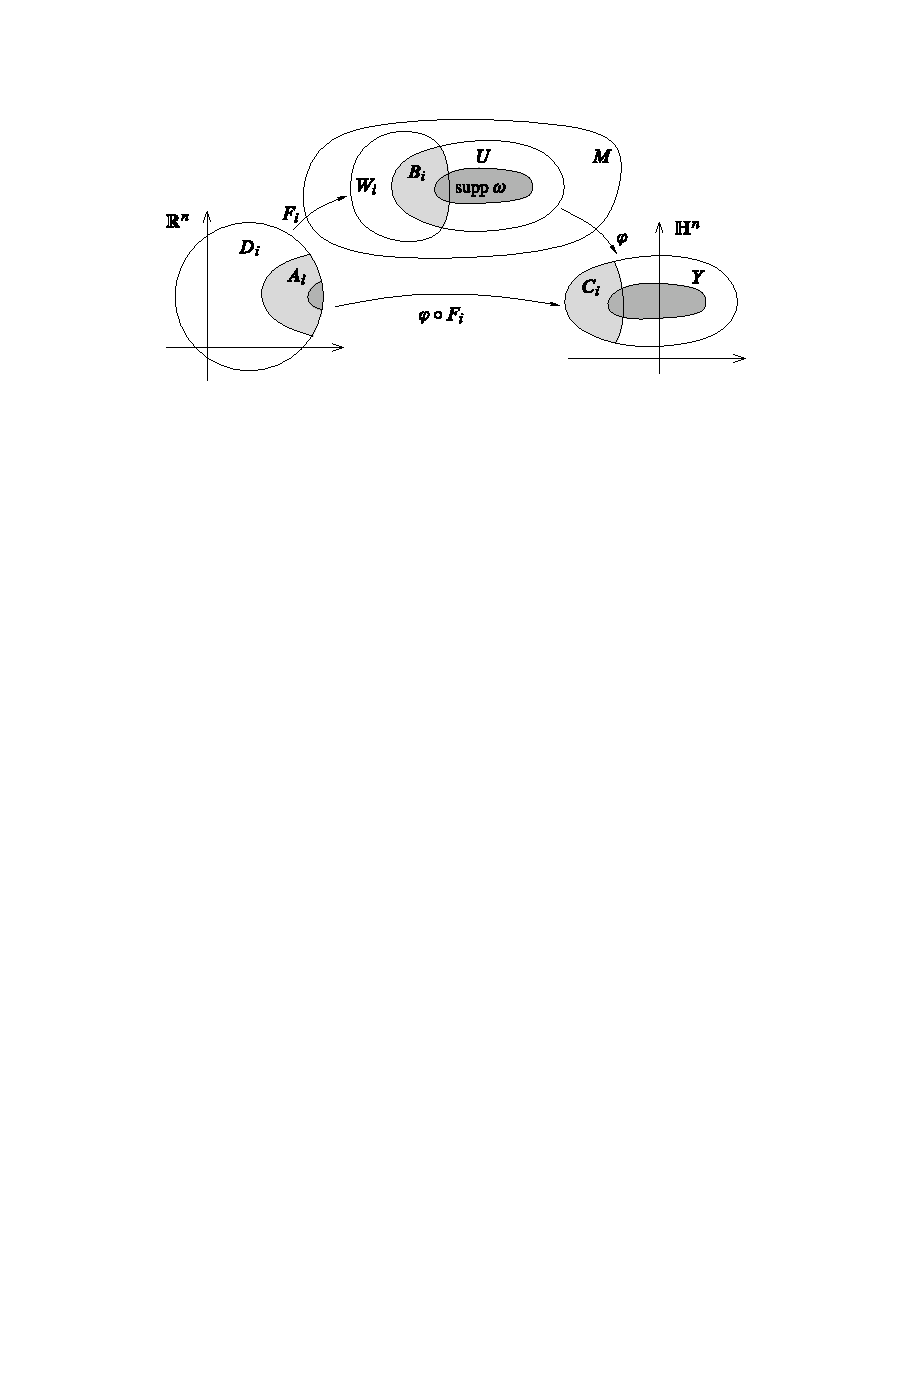
\includegraphics{pictures/int-form-para}
\caption{Integrating over parametrizations.}
\end{figure}
Because $\widebar{D}_i$ is compact, it is straightforward to check that $\partial W_i\sub F_i(\partial D_i)$, and therefore $\partial W_i$ has measure zero in $M$, and $\partial C_i=\varphi(\partial B_i)$ has measure zero in $\R^n$.\par
The support of $\varphi_*\omega$ is contained in $\bigcup_{i=1}^{k}\widebar{C}_i$, and any two of these sets intersect only on their boundaries, which have measure zero. Thus
\[\int_M\omega=\int_Y\varphi_*\omega=\sum_{i=1}^{k}\int_{C_i}\varphi_*\omega.\]
The proof is completed by applying Proposition~\ref{int R^n pull back} to each term above, using the diffeomorphism $\varphi\circ F_i:A_i\to C_i$:
\[\int_{C_i}\varphi_*\omega=\int_{A_i}(\varphi\circ F_i)^*\varphi_*\omega=\int_{A_i}F_i^*\omega=\int_{D_i}F_i^*\omega.\]
Summing over $i$, we obtain $(\ref{inte mani para-1})$.
\end{proof}
\begin{example}
Let us use this technique to compute the integral of a $2$-form over $S^2$, oriented as the boundary of $\widebar{B}^3$. Let $\omega$ be the following $2$-form on $\R^3$
\[\omega=x\,dy\wedge dz+y\,dz\wedge dx+z\,dx\wedge dy.\]
Let $D$ be the open rectangle $(0,\pi)\times(0,2\pi)$, and let $F:D\to S^2$ be the spherical coordinate parametrization $F(\varphi,\theta)=(\sin\varphi\cos\theta,\sin\varphi\sin\theta,\cos\theta)$. Example~\ref{orientation para eg} showed that $F|_D$ is orientation-preserving, so it satisfies the hypotheses of Proposition~\ref{int mani para}. Note that
\begin{flalign*}
&F^*dx=\cos\varphi\cos\theta\,d\varphi-\sin\varphi\sin\theta\,d\theta,\\
&F^*dy=\cos\varphi\sin\theta\,d\varphi+\sin\varphi\cos\theta\,d\theta,\\
&F^*dz=-\sin\varphi\,d\varphi.
\end{flalign*}
Therefore,
\begin{align*}
\int_{S^2}\omega=&\int_D\big(-\sin^3\varphi\cos^2\theta\,d\theta\wedge d\varphi+\sin^3\varphi\sin^2\theta\,d\varphi\wedge d\theta\\
&+\cos^3\varphi\sin\theta\cos^2\theta\,d\varphi\wedge d\theta-\cos^2\varphi\sin\varphi\sin^2\theta\,d\theta\wedge d\varphi\big)\\
=&\int_D\sin\varphi\,d\varphi\wedge d\theta=\int_{0}^{2\pi}\int_{0}^{\pi}\sin\varphi\,d\varphi d\theta=4\pi.
\end{align*}
\end{example}
\begin{remark}
It is worth remarking that the hypotheses of Proposition~\ref{int mani para} can be relaxed somewhat. The requirement that each map $F_i$ be smooth on $\widebar{D}_i$ is included to ensure that the boundaries of the image sets $W_i$ have measure zero and that the pullback forms $F^*\omega$ are continuous on $\widebar{D}_i$. Provided the open subsets $W_i$ together fill up all of $M$ except for a set of measure zero, we can allow maps $F_i$ that do not extend smoothly to the boundary, by interpreting the resulting integrals of unbounded forms either as improper Riemann integrals or as Lebesgue integrals. For example, if the closed upper hemisphere of $S^2$ is parametrized by the map $F:\widebar{B}^2\to S^2$ given by $F(u,v)=(u,v,\sqrt{1-u^2-v^2})$, then $F$ is continuous but not smooth up to the boundary, but the conclusion of the proposition still holds.
\end{remark}
\subsubsection{Integration on Lie groups}
Let $G$ be a Lie group. A covariant tensor field $A$ on $G$ is said to be \textbf{left-invariant} if $L_g^*A=A$ for all $g\in G$.
\begin{proposition}
Let $G$ be a compact Lie group endowed with a left-invariant orientation. Then $G$ has a unique positively oriented left-invariant $n$-form $\omega_G$ with the property that $\int_G\omega_G=1$.
\end{proposition}
\begin{proof}
If $\dim G=0$, we just let $\omega_G$ be the constant function $1/k$, where $k$ is the
cardinality of $G$. Otherwise, let $E_1,\dots,E_n$ be a left-invariant global frame on $G$ (i.e., a basis for the Lie algebra of $G$). By replacing $E_1$ with $-E_1$ if necessary, we may assume that this frame is positively oriented. Let $\eps^1,\dots,\eps^n$ be the dual coframe. Left invariance of $E_j$ implies that
\[(L_g^*)(E_j)=\eps^i\big(d(L_g)(E_j)\big)=\eps^i(E_j)=\delta^i_j,\]
which shows that $L_g^*\eps^i=\eps^i$, so $\eps^i$ is left-invariant.\par
Let $\omega_G=\eps^1\wedge\cdots\wedge\eps^n$. Then
\[L_g^*\omega_G=L_g^*\eps^1\wedge\cdots\wedge L_g^*\eps^n=\eps^1\wedge\cdots\wedge\eps^n=\omega_G,\]
so $\omega_G$ is left-invariant as well. Because $\omega_G(E_1,\dots,E_n)>0$, $\omega_G$ is an orientation form for the given orientation. Clearly, any positive constant multiple of $\omega_G$ is also a left-invariant orientation form. Conversely, if $\widetilde{\omega}_G$ is any other left-invariant orientation form, we can write $\widetilde{\omega}_G|_e=c\omega_G|_e$ for some positive number $c$. Using left-invariance, we find that
\[\widetilde{\omega}_G|_g=L_{g^{-1}}^*\widetilde{\omega}_G|_e=cL_{g^{-1}}^*\omega_G|_e=c\omega_G|_g,\]
which proves that $\widetilde{\omega}_G$ is a positive constant multiple of $\omega_G$.\par
Since $G$ is compact and oriented, $\int_G\omega_G$ is a positive real number, so we can define $\widetilde{\omega}_G=(\int_G\omega_G)^{-1}\omega_G$. Clearly, $\widetilde{\omega}_G$ is the unique positively oriented left-invariant orientation form with integral $1$.
\end{proof}
\begin{remark}
The orientation form whose existence is asserted in this proposition is called the \textbf{Haar volume form} on $G$. Similarly, the map $f\mapsto\int_Gf\omega_G$ is called the \textbf{Haar integral}. Observe that the proof above did not use the fact that $G$ was compact until the last paragraph; thus every Lie group has a left-invariant orientation form that is uniquely defined up to a constant multiple. It is only in the compact case, however, that we can use the volume normalization to single out a unique one.
\end{remark}
\subsection{Stokes's theorem}
\begin{theorem}[\textbf{Stokes's Theorem}]\label{Stokes}
Let $M$ be an oriented smooth n-manifold with boundary, and let $\omega$ be a compactly supported smooth $(n-1)$-form on $M$. Then
\begin{align}\label{Stokes-1}
\int_Md\omega=\int_{\partial M}\omega.
\end{align}
\end{theorem}
\begin{remark}
The statement of this theorem is concise and elegant, but it requires a bit of interpretation. First, as usual, $\partial M$ is understood to have the induced $($Stokes$)$ orientation, and the $\omega$ on the right-hand side is to be interpreted as $\iota_{\partial M}^*\omega$. If $\partial M=\emp$, then the right-hand side is to be interpreted as zero. When $M$ is $1$-dimensional, the right-hand integral is really just a finite sum.
\end{remark}
\begin{proof}
We begin with a very special case: suppose $M$ is the upper half-space $\H^n$ itself. Then because $\omega$ has compact support, there is a number $R>0$ such that $\supp(\omega)$ is contained in the rectangle $A=[-R,R]\times\cdots\times[-R,R]\times[0,R]$. We can write $\omega$ in standard coordinates as
\[\omega=\sum_{i=1}^{n}\omega_i\,dx^1\wedge\cdots\wedge\widehat{dx^i}\wedge\cdots\wedge dx^n.\]
where the hat means that $dx^i$ is omitted. Therefore,
\begin{align*}
d\omega&=\sum_{i=1}^{n}d\omega_i\wedge dx^1\wedge\cdots\wedge\widehat{dx^i}\wedge\cdots\wedge dx^n\\
&=\sum_{i,j=1}^{n}\frac{\partial\omega_i}{\partial x_j}dx^j\wedge dx^1\wedge\cdots\wedge\widehat{dx^i}\wedge\cdots\wedge dx^n\\
&=\sum_{i=1}^{n}(-1)^{i-1}\frac{\partial\omega_i}{\partial x^i}dx^1\wedge\cdots\wedge dx^n.
\end{align*}
Thus we compute
\begin{align*}
\int_{\H^n}d\omega&=\sum_{i=1}^{n}\int_{A}(-1)^{i-1}\frac{\partial\omega_i}{\partial x^i}dx^1\wedge\cdots\wedge dx^n\\
&=\sum_{i=1}^{n}(-1)^{i-1}\int_{0}^{R}\int_{-R}^{R}\cdots\int_{-R}^{R}\frac{\partial\omega_i}{\partial x^i}(x)\,dx^1\cdots dx^n.
\end{align*}
We can change the order of integration in each term so as to do the $x^i$ integration first. By the fundamental theorem of calculus, the terms for which $i\neq n$ reduce to
\begin{align*}
\sum_{i=1}^{n}(-1)^{i-1}&\int_{0}^{R}\int_{-R}^{R}\cdots\int_{-R}^{R}\frac{\partial\omega_i}{\partial x^i}(x)\,dx^1\cdots dx^n\\
&=\sum_{i=1}^{n}(-1)^{i-1}\int_{0}^{R}\int_{-R}^{R}\cdots\int_{-R}^{R}\frac{\partial\omega_i}{\partial x^i}(x)\,dx^idx^1\cdots\widehat{dx^i}\cdots dx^n\\
&=\sum_{i=1}^{n}(-1)^{i-1}\int_{0}^{R}\int_{-R}^{R}\cdots\int_{-R}^{R}\Big[\omega_i(x)\Big]\Big|^{x^i=R}_{x^i=-R}dx^1\cdots\widehat{dx^i}\cdots dx^n=0.
\end{align*}
because we have chosen $R$ large enough that $\omega=0$ when $x^i=R$. The only term that might not be zero is the one for which $i=n$. For that term we have
\begin{align}\label{Stokes-2}
\int_{\H^n}d\omega&=(-1)^{n-1}\int_{-R}^{R}\int_{-R}^{R}\cdots\int_{0}^{R}\frac{\partial\omega_n}{\partial x^n}(x)\,dx^ndx^1\cdots dx^{n-1} \notag\\
&=(-1)^{n-1}\int_{-R}^{R}\cdots\int_{-R}^{R}\Big[\omega_n(x)\Big]\Big|_{x^n=0}^{x^n=R}\,dx^ndx^1\cdots dx^{n-1} \notag\\
&=(-1)^{n}\int_{-R}^{R}\cdots\int_{-R}^{R}\omega_n(x^1,\dots,x^{n-1},0)\,dx^1\wedge\cdots\wedge dx^{n-1}.
\end{align}
because $\omega_n=R$ when $x^n=R$.\par
To compare this to the other side of $(\ref{Stokes-1})$, we compute as follows:
\begin{align*}
\int_{\partial\H^n}\omega=\sum_i\int_{A\cap\partial\H^n}\omega_i(x^1,\dots,x^{n-1},0)\,dx^1\wedge\cdots\wedge\widehat{dx^i}\wedge\cdots\wedge dx^{n}.
\end{align*}
Because $x^n$ vanishes on $\partial\H^n$, the pullback of $dx^n$ to the boundary is identically zero. Thus, the only term above that is nonzero is the one for which $i=n$, which becomes
\[\int_{\partial\H^n}\omega=\int_{A\cap\partial\H^n}\omega_n(x^1,\dots,x^{n-1},0)\,dx^1\wedge\cdots\wedge dx^{n-1}.\]
Taking into account the fact that the coordinates $(x^1,\dots,x^{n-1})$ are positively oriented for $\partial\H^n$ when $n$ is even and negatively oriented when $n$ is odd (Example~\ref{orientation induce H^n}), we find that this is equal to $(\ref{Stokes-2})$.\par
Next we consider another special case: $M=\R^n$. In this case, the support of $\omega$ is contained in a cube of the form $A=[-R,R]^n$. Exactly the same computation goes through, except that in this case the $i=n$ term vanishes like all the others, so the left-hand side of $(\ref{Stokes-1})$ is zero. Since $M$ has empty boundary in this case, the right-hand side is zero as well.\par
Now let $M$ be an arbitrary smooth manifold with boundary, but consider an $(n-1)$-form $\omega$ that is compactly supported in the domain of a single positively
or negatively oriented smooth chart $(U,\varphi)$. Assuming that $\varphi$ is a positively oriented boundary chart, the definition yields
\[\int_Md\omega=\int_{\H^n}\varphi_*d\omega=\int_{\H^n}d(\varphi_*\omega).\]
By the computation above, this is equal to
\begin{align}\label{Stokes-3}
\int_{\partial\H^n}\varphi_*\omega.
\end{align}
where $\partial\H^n$ is given the induced orientation. Since $d\varphi$ takes outward-pointing vectors on $\partial M$ to outward-pointing vectors on $\H^n$ (by Proposition~\ref{inward outward vector iff}), it follows that $\varphi|_{U\cap\partial M}$ is an orientation-preserving diffeomorphism onto $\varphi(U)\cap\partial\H^n$, and thus $(\ref{Stokes-3})$ is equal to $\int_{\partial M}\omega$. For a negatively oriented smooth boundary chart, the same argument applies with an additional negative sign on each side of the equation. For an interior chart, we get the the same computations with $\H^n$ replaced by $\R^n$. This proves the theorem in this case.\par
Finally, let $\omega$ be an arbitrary compactly supported smooth $(n-1)$-form. Choosing a cover of $\supp(\omega)$ by finitely many domains of positively or negatively oriented smooth charts $\{U_i\}$, and choosing a subordinate smooth partition of unity $\{\psi_i\}$, we can apply the preceding argument to $\psi_i\omega$ for each $i$ and obtain
\begin{align*}
\int_{\partial M}\omega&=\sum_i\int_{\partial M}\psi_i\omega=\sum_i\int_Md(\psi_i\omega)=\sum_i\int_Md\psi_i\,\omega+\psi_i\,d\omega\\
&=\int_Md\Big(\sum_i\psi_i\Big)\omega+\int_M\Big(\sum_i\psi_i\Big)d\omega=\int_Md\omega.
\end{align*}
because $\sum_i\psi_i\equiv 1$.
\end{proof}
\begin{example}
Let $M$ be a smooth manifold and suppose $\gamma:[a,b]\to M$ is a smooth embedding, so that $S=\gamma([a,b])$ is an embedded $1$-submanifold with boundary in $M$. If we give $S$ the orientation such that $\gamma$ is orientation-preserving, then for any smooth function $f\in C^\infty(M)$, Stokes's theorem says that
\[\int_{\gamma}df=\int_{[a,b]}\gamma^*f=\int_{S}df=\int_{\partial S}f=f\big(\gamma(b)\big)-f\big(\gamma(a)\big).\]
\end{example}
Two special cases of Stokes's theorem arise so frequently that they are worthy of special note. The proofs are immediate.
\begin{corollary}[\textbf{Integrals of Exact Forms}]\label{int exact form}
If $M$ is a compact oriented smooth manifold without boundary, then the integral of every exact form over $M$ is zero:
\[\int_Md\omega=0\quad\text{if }\partial M=\emp.\]
\end{corollary}
\begin{corollary}[\textbf{Integrals of Closed Forms over Boundaries}]\label{int closed form}
Suppose $M$ is a compact oriented smooth manifold with boundary. If $\omega$ is a closed form on $M$, then the integral of $\omega$ over $\partial M$ is zero:
\[\int_{\partial M}\omega=0\quad\text{if }d\omega=0.\]
\end{corollary}
These results have the following extremely useful applications to submanifolds.
\begin{corollary}
Suppose $M$ is a smooth manifold with or without boundary, $S\sub M$ is an oriented compact smooth $k$-dimensional submanifold (without boundary), and $\omega$ is a closed $k$-form on $M$. If $\int_S\omega\neq0$, then both of the following are
true:
\begin{itemize}
\item[(a)] $\omega$ is not exact on $M$.
\item[(b)] $S$ is not the boundary of an oriented compact smooth submanifold with boundary in $M$.
\end{itemize}
\end{corollary}
\begin{example}
It follows from the computation of Example~\ref{covector closed not exact eg} that the closed $1$-form 
\[\omega=\frac{x\,dy-y\,dx}{x^2+y^2}\]
has nonzero integral over $S^1$. We already observed that $\omega$ is not exact on $\R^2-\{0\}$. The preceding corollary tells us in addition that $S^1$ is not the boundary of a compact regular domain in $\R^2-\{0\}$.
\end{example}
The following classical result is an easy application of Stokes's theorem.
\begin{theorem}[\textbf{Green's Theorem}]
Suppose $D$ is a compact regular domain in $\R^2$, and $P,Q$ are smooth real-valued functions on $D$. Then
\[\int_D\Big(\frac{\partial Q}{\partial x}-\frac{\partial P}{\partial y}\Big)dxdy=\int_{\partial D}P\,dx+Q\,dy.\]
\end{theorem}
\subsection{Manifolds with corners}
In many applications of Stokes's theorem it is necessary to deal with geometric objects such as triangles, squares, or cubes that are topological manifolds with boundary, but are not smooth manifolds with boundary because they have \textit{corners}. It is easy to generalize Stokes's theorem to this setting, and we do so in this section.\par
Let $\widebar{\R}^n_+$ denote the subset of $\R^n$ where all of the coordinates are nonnegative:
\[\widebar{\R}^n_+=\{(x^1,\dots,x^n)\in\R^n:x^1\geq 0,\dots,x^n\geq0\}.\]
This space is the model for the type of corners we are concerned with.
\begin{proposition}
The set $\widebar{\R}^n_+$ is homeomorphic to the upper half-space $\H^n$.
\end{proposition}
\begin{proof}
The homeomorphism $\varphi:\widebar{\R}^n_+\to\H^n$ is given by
\[\varphi(x^1,\dots,x^n)=(e^{x^1},\dots,e^{x^{n-1}},x^n).\]
\end{proof}
Suppose $M$ is a topological $n$-manifold with boundary. A \textbf{chart with corners} for $M$ is a pair $(U,\varphi)$, where $U\sub M$ is open and $\varphi$ is a homeomorphism from $U$ to a (relatively) open subset $\widehat{U}\sub\widebar{\R}^n_+$. Two charts with corners $(U,\varphi)$, $(V,\psi)$ are smoothly compatible if the composite map $\varphi\circ\psi^{-1}:\psi(U\cap V)\to \varphi(U\cap V)$ is smooth. (As usual, this means that it admits a smooth extension in an open neighborhood of each point.)\par
A \textbf{smooth structure} with corners on a topological manifold with boundary is a maximal collection of smoothly compatible interior charts and charts with corners
whose domains cover $M$. A topological manifold with boundary together with a smooth structure with corners is called a \textbf{smooth manifold with corners}. Any chart with corners in the given smooth structure with corners is called a \textbf{smooth chart with corners} for $M$.
\begin{example}
Any closed rectangle in $\R^n$ is a smooth $n$-manifold with corners.
\end{example}
The \textbf{boundary} of $\widebar{\R}^n_+$ in $\R^n$ is the set of points at which at least one coordinate vanishes. The points in $\widebar{\R}^n_+$ at which more than one coordinate vanishes are called its \textbf{corner points}. For example, the corner points of $\widebar{\R}^3_+$ are the origin together with all the points on the positive $x$-, $y$-, and $z$-axes.
\begin{proposition}[\textbf{Invariance of Corner Points}]
Let $M$ be a smooth $n$-manifold with corners, $n\geq 2$, and let $p\in M$. If $\varphi(p)$ is a corner point for some smooth chart with corners $(U,\varphi)$, then the same is true for every such chart whose domain contains $p$.
\end{proposition}
\begin{figure}[htbp]
\centering
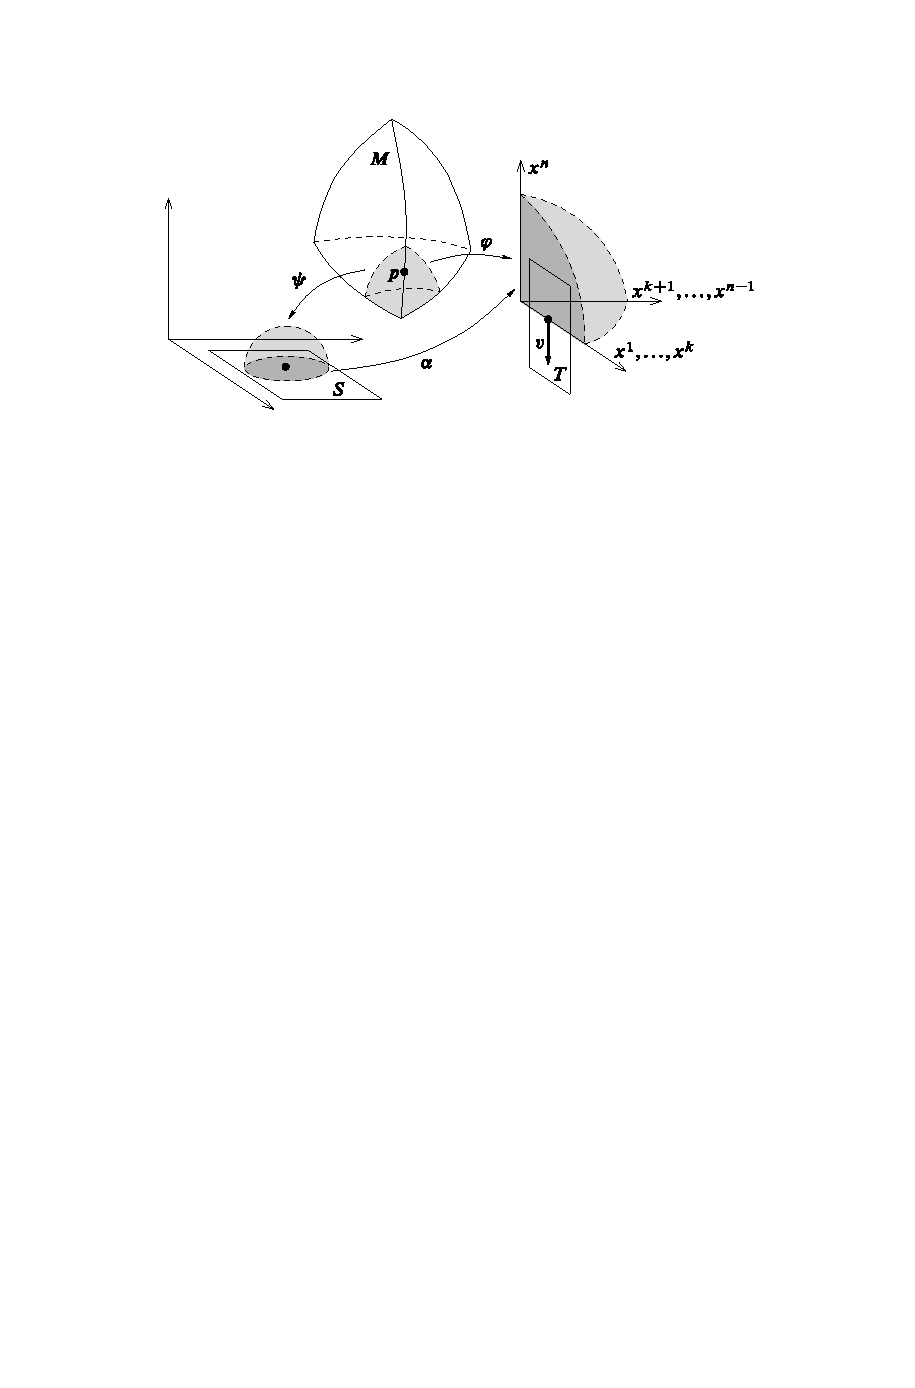
\includegraphics{pictures/inv-corner}
\caption{Invariance of corner points.}
\end{figure}
\begin{proof}
Suppose $(U,\varphi)$ and $(V,\psi)$ are two smooth charts with corners such that $\varphi(p)$ is a corner point but $\psi(p)$ is not. To simplify notation, let us
assume without loss of generality that $\varphi(p)$ has coordinates $(x^1,\dots,x^k,0,\dots,0)$ with $k\leq n-2$. Then $\psi(V)$ contains an open subset of some $(n-1)$-dimensional linear subspace $S\sub\R^n$, with $\psi(p)\in S$. (If $\psi(p)\in\partial\widebar{\R}^n_+$, take $S$ to be the unique subspace defined by an equation of the form $x^i=0$ that contains $\psi(p)$. If $\psi(p)$ is an interior point, any $(n-1)$-dimensional subspace containing $\psi(p)$ will do.)\par
Let $S'=S\cap\psi(U\cap V)$, and let $\alpha:S'\to\R^n$ be the restriction of $\varphi\circ\psi^{-1}$ to $S'$. Because $\varphi\circ\psi^{-1}$ is a diffeomorphism from $\psi(U\cap V)$ to $\varphi(U\cap V)$, it follows that $\psi\circ\varphi^{-1}\circ\alpha$ is the identity of $S'$, and therefore $d\alpha_{\psi(p)}$ is an injective linear map. Let $T=d\alpha_{\psi(p)}(T_{\psi(p)}S)\sub\R^n$. Because $T$ is $(n-1)$-dimensional, it must contain a vector $v$ such that one of the last two components, $v^{n-1}$ or $v^n$, is nonzero (otherwise, $T$ would be contained in a codimension-$2$ subspace). Renumbering the coordinates and replacing $v$ by $-v$ if necessary, we may assume that $v^n<0$.\par
Now let $\gamma:(-\eps,\eps)\to S$ be a smooth curve such that $\gamma(0)=p$ and $d\alpha(\gamma'(0))=v$. Then $\alpha\circ\gamma(t)$ has negative $x^n$ coordinate for small $t>0$, which contradicts the fact that $\alpha$ takes its values in $\widebar{\R}^n_+$.
\end{proof}
If $M$ is a smooth manifold with corners, a point $p\in M$ is called a corner point if $\varphi(p)$ is a corner point in $\widebar{\R}^n_+$ with respect to some (and hence every) smooth chart with corners $(U,\varphi(p))$. Similarly, $p$ is called a boundary point if $\varphi(p)\in\partial\widebar{\R}^n_+$ with respect to some (hence every) such chart. For example, the set of corner points of the unit cube $[0,1]^3\sub\R^3$ is the union of its eight vertices and twelve edges.\par
Every smooth manifold with or without boundary is also a smooth manifold with corners (but with no corner points). Conversely, a smooth manifold with corners is a
smooth manifold with boundary if and only if it has no corner points. The boundary of a smooth manifold with corners, however, is in general not a smooth manifold
with corners (e.g., think of the boundary of a cube). In fact, even the boundary of $\widebar{\R}^n_+$ itself is not a smooth manifold with corners. It is, however, a union of finitely many such: $\partial\widebar{\R}^n_+=H_1\cup\cdots\cup H_n$, where
\begin{align}\label{mani corner-1}
H_i=\{(x^1,\dots,x^n)\in\widebar{\R}^n_+:x^i=0\}
\end{align}
is an $(n-1)$-dimensional smooth manifold with corners contained in the subspace defined by $x^i=0$.\par
The usual flora and fauna of smooth manifolds—smooth maps, partitions of
unity, tangent vectors, covectors, tensors, differential forms, orientations, and integrals of differential forms—can be defined on smooth manifolds with corners in
exactly the same way as we have done for smooth manifolds and smooth manifolds
with boundary, using smooth charts with corners in place of smooth boundary
charts.\par
In addition, for Stokes's theorem we need to integrate a differential form over the boundary of a smooth manifold with corners. Since the boundary is not itself a smooth manifold with corners, this requires a separate (albeit routine) definition.\par 
Let $M$ be an oriented smooth $n$-manifold with corners, and suppose $\omega$ is an $(n-1)$-form on $\partial M$ that is compactly supported in the domain of a single chart with corners $(U,\varphi)$. We define the integral of $\omega$ over $\partial M$ by
\[\int_{\partial M}\omega=\sum_{i=1}^{n}\int_{H_i}\varphi_*\omega,\]
where $H_i$, defined by $(\ref{mani corner-1})$, is given the induced orientation as part of the boundary of the set where $x^i\geq0$. In other words, we simply integrate $\omega$ in coordinates over the codimension-$1$ portion of the boundary.\par 
Finally, if $\omega$ is an arbitrary compactly supported $(n-1)$-form on $M$, we define the integral of $\omega$ over $\partial M$ by piecing together with a partition of unity just as in the case of a manifold with boundary.\par
In practice, of course, one does not evaluate such integrals by using partitions of unity. Instead, one chops up the boundary into pieces that can be parametrized by open subsets, just as for ordinary manifolds with or without boundary. The following proposition is an analogue of Proposition~\ref{int mani para}.
\begin{proposition}
The statement of Proposition~\ref{int mani para} is true if $M$ is replaced by the boundary of a oriented smooth $(n+1)$-manifold with corners.
\end{proposition}
\begin{example}\label{squre para}
Let $I\times I=[0,1]^2\sub\R^2$ be the unit square in $\R^2$, and suppose $\omega$ is a $1$-form on $\partial(I\times I)$. Then it is not hard to check that the maps $F_i:I\to I\times I$ given by
\begin{equation}\label{squre para-1}
\begin{array}{ll}
F_1(t)=(t,0),&F_2(t)=(1,t),\\
F_3(t)=(1-t,1),&F_4(t)=(0,-t).
\end{array}
\end{equation}
satisfy the hypotheses of Proposition~\ref{int mani para}. Therefore,
\[\int_{\partial(I\times I)}\omega=\int_{F_1}\omega+\int_{F_2}\omega+\int_{F_3}\omega+\int_{F_4}\omega.\]
\end{example}
\begin{theorem}[\textbf{Stokes's Theorem on Manifolds with Corners}]
Let $M$ be an oriented smooth $n$-manifold with corners, and let $\omega$ be a compactly supported smooth $(n-1)$-form on $M$. Then
\[\int_Md\omega=\int_{\partial M}\omega.\]
\end{theorem}
\begin{proof}
The proof is nearly identical to the proof of Stokes's theorem proper, so we just indicate where changes need to be made. By means of smooth charts and a partition of unity, we may reduce the theorem to the case in which either $M=\R^n,\H^n$ or $M=\widebar{\R}^n_+$. The $\R^n$ and $\H^n$ case are treated just as before. In the case of a chart with corners, $\omega$ is supported in some cube $[0,R]^n$, and we calculate exactly as in the proof of Theorem~\ref{Stokes}:
\begin{align*}
\int_{\widebar{\R}^n_+}d\omega&=\sum_{i=1}^{n}(-1)^{i-1}\int_{0}^{R}\cdots\int_{0}^{R}\frac{\partial\omega_i}{\partial x^i}(x)\,dx^1\cdots dx^n\\
&=\sum_{i=1}^{n}(-1)^{i-1}\int_{0}^{R}\cdots\int_{0}^{R}\frac{\partial\omega_i}{\partial x^i}(x)\,dx^idx^1\cdots\widehat{dx^i}\cdots dx^n\\
&=\sum_{i=1}^{n}(-1)^{i-1}\int_{0}^{R}\cdots\int_{0}^{R}\Big[\omega_i(x)\Big]\Big|_{x^i=0}^{x^i=R}dx^1\cdots\widehat{dx^i}\cdots dx^n\\
&=\sum_{i=1}^{n}(-1)^{i}\int_{0}^{R}\cdots\int_{0}^{R}\omega_i(x^1,\dots,0,\dots,x^n)\,dx^1\cdots\widehat{dx^i}\cdots dx^n\\
&=\sum_{i=1}^{n}\int_{H_i}\omega=\int_{\partial\widebar{\R}^n_+}\omega.
\end{align*}
(The factor $(-1)^i$ disappeared because the induced orientation on $H_i$ is $(-1)^i$ times that of the standard coordinates $(x^1,\dots,\widehat{x^i},\dots,x^n)$) This completes the proof.
\end{proof}
The preceding theorem has the following important application.
\begin{theorem}\label{int homotopy path}
Suppose $M$ is a smooth manifold and $\gamma_0,\gamma_1:[a,b]\to M$ are path-homotopic piecewise smooth curve segments. For every closed $1$-form $\omega$ on $M$,
\[\int_{\gamma_0}\omega=\int_{\gamma_1}\omega.\]
\end{theorem}
\begin{proof}
By means of an affine reparametrization, we may as well assume for simplicity that $[a,b]=[0,1]$. Assume first that $\gamma_0$ and $\gamma_1$ are smooth. By Theorem~\ref{homotopy to smooth}, $\gamma_0$ and $\gamma_1$ are smoothly homotopic relative to $\{0,1\}$. Let $H:I\times I\to M$ be such a smooth homotopy. Since $\omega$ is closed, we have
\[\int_{I\times I}d(H^*\omega)=\int_{I\times I}H^*d\omega=0.\]
On the other hand, $I\times I$ is a smooth manifold with corners, so Stokes's theorem
implies
\[0=\int_{I\times I}d(H^*\omega)=\int_{\partial(I\times I)}H^*\omega.\]
Using the parametrization of $\partial(I\times I)$ given in Example~\ref{squre para} together with Proposition~\ref{line integral prop}, we obtain
\begin{align*}
0&=\int_{\partial(I\times I)}H^*\omega=\int_{\partial(I\times I)}H^*\omega=\int_{F_1}H^*\omega+\int_{F_2}H^*\omega+\int_{F_3}H^*\omega+\int_{F_4}H^*\omega\\
&=\int_{H\circ F_1}\omega+\int_{H\circ F_2}\omega+\int_{H\circ F_3}\omega+\int_{H\circ F_4}\omega.
\end{align*}
The fact that $H$ is a homotopy relative to $\{0,1\}$ means that $H\circ F_2$ and $H\circ F_4$ are constant maps, and therefore the second and fourth terms above are zero. The theorem then follows from the facts that $H\circ F_1=\gamma_0$ and $H\circ F_3$ is a backward reparametrization of $\gamma_1$.\par
Next we consider the general case of piecewise smooth curves.We cannot simply
apply the preceding result on each subinterval where $\gamma_0$ and $\gamma_1$ are smooth, because the restricted curves may not start and end at the same points. Instead, we prove the following more general claim: Let $\gamma_0,\gamma_1:[0,1]\to M$ be piecewise smooth curve segments (not necessarily with the same endpoints), and suppose $H:I\times I\to M$ is any homotopy between them. Define curve segments $\sigma_0,\sigma_1:I\to M$ by
\[\sigma_0(t)=H(0,t),\quad \sigma_1(t)=H(1,t),\]
and let $\widetilde{\sigma}_0,\widetilde{\sigma}_1$ be any smooth curve segments that are path-homotopic to $\sigma_0,\sigma_1$ respectively. Then
\begin{align}\label{int homotopy-1}
\int_{\gamma_1}\omega-\int_{\gamma_0}\omega=\int_{\widetilde{\sigma}_1}\omega-\int_{\widetilde{\sigma}_0}\omega.
\end{align}
When specialized to the case in which $\gamma_0$ and $\gamma_1$ are path-homotopic, this implies the theorem, because $\gamma_0$ and $\gamma_1$ are constant maps in that case.\par
Since $\gamma_0$ and $\gamma_1$ are piecewise smooth, there are only finitely many points $\{a_1,\dots,a_m\}$ in $[0,1]$ at which either $\gamma_0$ or $\gamma_1$ is not smooth. We prove the claim by induction on the number $m$ of such points. When $m=0$, both curves are smooth, and by Theorem~\ref{homotopy to smooth} we may replace the given homotopy $H$ by a smooth homotopy $\widetilde{H}$. Recall from the proof of Theorem~\ref{homotopy to smooth} that the smooth homotopy $\widetilde{H}$ can actually be taken to be homotopic to $H$ relative to $I\times\{0\}\cup I\times\{1\}$. Thus, for $i=0,1$, the curve $\widetilde{\sigma}_i=\widetilde{H}(i,t)$ is a smooth curve segment that is path-homotopic to $\sigma_i$. In this setting, $(\ref{int homotopy-1})$ just reduces to the integration formula of Example~\ref{squre para}. Note that the integrals over $\widetilde{\sigma}_0$ and $\widetilde{\sigma}_1$ do not depend on which smooth curves pathhomotopic to $\sigma_0$ and $\sigma_1$ are chosen, by the smooth case proved above.\par
Now let $\gamma_0,\gamma_1$ be homotopic piecewise smooth curves with $m$ nonsmooth points $\{a_1,\dots,a_m\}$, and suppose the claim is true for curves with fewer than $m$ such points. For $i=0,1$, let $\gamma'_i$ be the restriction of $\gamma_i$ to $[0,a_m]$, and let $\gamma''_i$ be its restriction to $[a_m,1]$. Let $\sigma:I\to M$ be the curve segment $\sigma(t)=H(a_m,t)$, and let $\widetilde{\sigma}$ by any smooth curve segment that is path-homotopic to $\sigma$. Then, since $\gamma'_i$ and $\gamma''_i$ have fewer than $m$ nonsmooth points, the inductive hypothesis implies
\begin{align*}
\int_{\gamma_1}\omega-\int_{\gamma_0}\omega&=\Big(\int_{\gamma'_1}\omega+\int_{\gamma''_1}\omega\Big)-\Big(\int_{\gamma'_0}\omega+\int_{\gamma''_0}\omega\Big)\\
&=\Big(\int_{\gamma'_1}\omega-\int_{\gamma'_0}\omega\Big)+\Big(\int_{\gamma''_1}\omega+\int_{\gamma''_1}\omega\Big)\\
&=\Big(\int_{\widetilde{\sigma}}\omega-\int_{\widetilde{\sigma}_0}\omega\Big)+\Big(\int_{\widetilde{\sigma}_1}\omega+\int_{\widetilde{\sigma}}\omega\Big)\\
&=\int_{\widetilde{\sigma}_1}\omega-\int_{\widetilde{\sigma}_0}\omega.
\end{align*}
\end{proof}
\begin{corollary}\label{simply con 1 form}
On a simply connected smooth manifold, every closed $1$-form is exact.
\end{corollary}
\begin{proof}
Suppose $M$ is simply connected and $\omega$ is a closed $1$-form on $M$. Since every piecewise smooth closed curve segment in $M$ is path-homotopic to a constant curve,
the preceding theorem shows that the integral of $\omega$ over every such curve is equal to $0$. Thus, $\omega$ is conservative and therefore exact.
\end{proof}
\subsection{Integration on Riemannian manifolds}
\subsubsection{Integration of functions on Riemannian manifolds}
Suppose $(M,g)$ is an oriented Riemannian manifold with or without boundary, and let $\omega_g$ denote its Riemannian volume form. If $f$ is a compactly supported continuous real-valued function on $M$, then $f\omega_g$ is a compactly supported $n$-form, so we can define the \textbf{integral of $\bm{f}$ over $\bm{M}$} to be $\int_Mf\omega_g$. If $M$ itself is compact, we define the \textbf{volume of $\bm{M}$} by $\mathrm{Vol}(M)=\int_M\omega_g$.\par
Because of these definitions, the Riemannian volume form is often denoted by $dV_g$ (or $dA_g$ or $ds_g$ in the $2$-dimensional or $1$-dimensional case, respectively). Then the integral of $f$ over $M$ is written $\int_M f\,dV_g$, and the volume of $M$ as $\int_MdV_g$. Be warned, however, that this notation is not meant to imply that the volume form is the exterior derivative of an $(n-1)$-form; in fact, as we will see when we study de Rham cohomology, this is never the case on a compact manifold. You should just interpret $dV_g$ as a notational convenience.
\begin{proposition}
Let $(M,g)$ be a nonempty oriented Riemannian manifold with or without boundary, and suppose $f$ is a compactly supported continuous realvalued function on $M$ satisfying $f\geq0$. Then $\int_Mf\,dV_g\geq0$, with equality if and only if $f\equiv 0$.
\end{proposition}
\begin{proof}
If $f$ is supported in the domain of a single oriented smooth chart $(U,\varphi)$, then Proposition~\ref{Riemannian volume form} shows that
\[\int_Mf\,dV_g=\int_Mf\sqrt{G}\,dx^1\cdots dx^n\geq0.\]
The same inequality holds in a negatively oriented chart because the negative sign from the chart cancels the negative sign in the expression for $dV_g$. The general case follows from this one, because $\int_Mf\,dV_g$ is equal to a sum of terms like
$\int_M\psi f\,dV_g$, where each integrand if is nonnegative and supported in a single
smooth chart. If in addition $f$ is positive somewhere, then it is positive on a nonempty open subset by continuity, so at least one of the integrals in this sum is
positive. On the other hand, if $f$ is identically zero, then clearly $\int_Mf\,dV_g=0$.
\end{proof}
In the same way, we can prove the following result.
\begin{proposition}
Suppose $(M,g)$ is an oriented Riemannian manifold and $f:M\to\R$ is continuous and compactly supported. Then
\[\Big|\int_Mf\,dV_g\Big|\leq\int_M|f|\,dV_g.\]
\end{proposition}
\subsubsection{The divergence theorem}
Let $(M,g)$ be an oriented Riemannian $n$-manifold (with or without boundary). We can generalize the classical divergence operator to this setting as follows. Multiplication by the Riemannian volume form defines a smooth bundle isomorphism $\ast:C^\infty(M)\to\Omega^n(M)$:
\[\ast f:=f\,dV_g.\]
In addition, as we did in the case of $\R^3$, we define a smooth bundle isomorphism $\beta:\X(M)\to\Omega^{n-1}(M)$ as follows:
\begin{align}\label{int prod Riemann}
\beta(X)=X\intprod dV_g.
\end{align}
We need the following technical lemma.
\begin{lemma}~\label{divergence lemma}
Let $(M,g)$ be an oriented Riemannian manifold with or without boundary. Suppose $S\sub M$ is an immersed hypersurface with the orientation determined by a unit normal vector field $N$, and $\widetilde{g}$ is the induced metric on $S$. If $X$ is any vector field along $S$, then
\begin{align}\label{div lem-1}
\iota_S^*(\beta(X))=\langle X,N\rangle_gdV_{\widetilde{g}}.
\end{align}
\end{lemma}
\begin{proof}
Define two vector fields $X$ and $X$ along $S$ by
\[X^\bot=\langle X,N\rangle_gN,\quad X^\top=X-X^\bot.\]
Then $X=X^\bot+X^\top$, where $X^\bot$ is normal to $S$ and $X^\top$ is tangent to it. Using this decomposition,
\[\beta(X)=X^\bot\intprod dV_g+X^\top\intprod dV_g.\]
Now pull back to $S$. Proposition~\ref{Riemann volumn form hyper} shows that the first term simplifies to
\[\iota_S^*(X^\bot\intprod dV_g)=\langle X,N\rangle_g\iota_S^*(N\intprod dV_g)=\langle X,N\rangle_g\,dV_{\widetilde{g}}.\]
Thus $(\ref{div lem-1})$ will be proved if we can show that $\iota_S^*(X^\top\intprod dV_g)=0$. If $X_1,\dots,X_{n-1}$ are any vectors tangent to $S$, then
\[(X^\top\intprod dV_g)(X_1,\dots,X_{n-1})=dV_g(X,X_1,\dots,X_{n-1})=0,\]
because any $n$-tuple of vectors in an $(n-1)$-dimensional vector space is linearly
dependent.
\end{proof}
Now we define the \textbf{divergence operator} $\div:\X(M)\to C^\infty(M)$ by
\begin{align}\label{div def-1}
\div X=\ast^{-1}d(\beta(X))=\ast^{-1}d(X\intprod dV_g).
\end{align}
or equivalently,
\begin{align}\label{div def-2}
d(X\intprod dV_g)=(\div X)dV_g.
\end{align}
Even if $M$ is nonorientable, in a neighborhood of each point we can choose an orientation and define the divergence by $(\ref{div def-2})$, and then note that reversing the orientation changes the sign of $dV_g$ on both sides of the equation, so $\div X$ is well defined, independently of the choice of orientation. In this way, we can define the divergence operator on any Riemannian manifold with or without boundary, by requiring that it satisfy $(\ref{div def-2})$ for any choice of orientation in a neighborhood of each point.\par
The next theorem is a fundamental result about vector fields on Riemannian manifolds. In the special case of a compact regular domain in $\R^3$, it is often referred to as \textbf{Gauss's theorem}.
\begin{theorem}[\textbf{The Divergence Theorem}]
Let $(M,g)$ be an oriented Riemannian manifold with boundary. For any compactly supported smooth vector field $X$ on $M$,
\[\int_M(\div X)\,dV_g=\int_{\partial M}\langle N,X\rangle_g\,dV_{\widetilde{g}}.\]
where $N$ is the outward-pointing unit normal vector field along $\partial M$ and $\widetilde{g}$ is the induced Riemannian metric on $\partial M$.
\end{theorem}
\begin{proof}
By Stokes's theorem,
\[\int_M(\div X)\,dV_g=\int_Md(\beta(X))=\int_{\partial M}\iota^*_{\partial M}\beta(X).\]
The divergence theorem then follows from Lemma~\ref{divergence lemma}.
\end{proof}
The term divergence is used because of the following geometric interpretation. A smooth flow $\theta$ on $M$ is said to be volume-preserving if for every compact regular domain $D$, we have $\mathrm{Vol}(\theta_t(D))=\mathrm{Vol}(D)$ whenever the domain of $\theta_t$ contains $D$. It is called \textbf{volume-increasing}, \textbf{volume-decreasing}, \textbf{volume-nonincreasing}, or \textbf{volume-nondecreasing} if for every such $D$, $\mathrm{Vol}(\theta_t(D))$ is strictly increasing, strictly decreasing, nonincreasing, or nondecreasing, respectively, as a function of $t$. Note that the properties of flow domains ensure that if $D$ is contained in the domain of $\theta_t$ for some $t$, then the same is true for all times between $0$ and $t$.\par
The next proposition shows that the divergence of a vector field can be interpreted as a measure of the tendency of its flow to spread out.
\begin{proposition}[\textbf{Geometric Interpretation of the Divergence}]\label{divergence geometric interpretation}
Let $M$ be an oriented Riemannian manifold, let $X\in\X(M)$, and let $\theta$ be the flow of $X$. Then $\theta$ is
\begin{itemize}
\item[(a)] volume-preserving if and only if $\div X=0$ everywhere on $M$.
\item[(b)] volume-nondecreasing if and only if $\div X=0$ everywhere on $M$.
\item[(c)] volume-nonincreasing if and only if $\div X\geq0$ everywhere on $M$.
\item[(d)] volume-increasing if and only if $\div X>0$ on a dense subset of $M$.
\item[(e)] volume-decreasing if and only if $\div X<0$ on a dense subset of $M$.
\end{itemize}
\end{proposition}
\begin{proof}
First we establish some preliminary results. For each $t\in\R$, let $M_t$ be the domain of $\theta_t$. If $D$ is a compact regular domain contained in $M_t$, then $\theta_t$ is an orientation-preserving diffeomorphism from $D$ to $\theta_t(D)$ by the result of Exercise~\ref{orientation flow}, so
\[\mathrm{Vol}(\theta_t(D))=\int_{\theta_t(D)}dV_g=\int_D\theta_t^*dV_g.\]
Because the integrand on the right depends smoothly on $(t,p)$ in the domain of $\theta$, we can differentiate this expression with respect to $t$ by differentiating under the integral sign.\par
Using Cartan's magic formula for the Lie derivative of the Riemannian volume form, we obtain
\[\mathfrak{L}_XdV_g=X\intprod d(dV_g)+d(X\intprod dV_g)=(\div X)dV_g.\]
because $d(dV_g)$ is an $(n+1)$-form on an $n$-manifold. Then Proposition~\ref{Lie der tensor t_0} implies
\begin{align*}
\frac{d}{dt}\Big|_{t=t_0}\mathrm{Vol}(\theta_t(D))&=\int_{D}\frac{\partial}{\partial t}\Big|_{t=t_0}(\theta_t^*dV_g)=\int_D\theta_{t_0}^*(\mathfrak{L}_XdV_g)\\
&=\int_D\theta_{t_0}^*((\div X)dV_g)=\int_{\theta_{t_0}(D)}(\div X)dV_g.
\end{align*}
From this, the claim is easily proved.
\end{proof}
Using the divergence operator, we can define another important operator. The \textbf{Laplacian} (or \textbf{Laplace–Beltrami operator}) is the linear operator $\Delta:C^{\infty}(M)\to C^{\infty}(M)$ defined by
\begin{align}\label{Laplacian def}
\Delta f=\div(\grad f).
\end{align}
The next proposition gives alternative formulas for these operators.
\begin{proposition}
Let $(M,g)$ be a Riemannian manifold with or without boundary, and let $(x^i)$ be any smooth local coordinates on an open set $U\sub M$. The coordinate representations of the divergence and Laplacian are as follows:
\begin{align}\label{div coordinate}
\div(X^i\frac{\partial}{\partial x^i})=\frac{1}{\sqrt{G}}\frac{\partial}{\partial x^i}\Big(\sqrt{G}X^i\Big)
\end{align}
\begin{align}\label{Laplacian coordinate}
\Delta f=\frac{1}{\sqrt{G}}\frac{\partial}{\partial x^i}\Big(\sqrt{G}g^{ij}\frac{\partial f}{\partial x^j}\Big).
\end{align}
where $G=\det(g_{ij})$ is the determinant of the component matrix of $g$ in these coordinates.
\end{proposition}
\begin{proof}
By Proposition~\ref{Riemann volume form formula} 2e have
\[X\intprod dV_g=X\intprod\sqrt{G}\, dx^1\wedge\cdots\wedge dx^n=\sqrt{G}\sum_{i=1}^{n}(-1)^{n-1}X^i\, dx^1\wedge\cdots\widehat{dx^i}\wedge\cdots\wedge dx^n.\]
Therefore
\[d(X\intprod dV_g)=\frac{\partial}{\partial x^i}\Big(\sqrt{G}X^i\Big)dx^1\wedge\cdots dx^n=\frac{1}{\sqrt{G}}\frac{\partial}{\partial x^i}\Big(\sqrt{G}X^i\Big)dV_g,\]
and so $(\ref{div coordinate})$ holds. The second formula follows from the expression of $\grad f$.
\end{proof}
\subsubsection{Surface integrals}
The original theorem that bears the name of Stokes concerned surface integrals of vector fields over surfaces in $\R^3$. Using the version of Stokes's theorem that we have proved, we cam generalize this to surfaces in Riemannian $3$-manifolds.\par 
Let $(M,g)$ be an oriented Riemannian $3$-manifold. Define the $\curl$ operator, denoted by $\curl:\X(M)\to\X(M)$ by
\[\curl X=\beta^{-1}d(X^\flat),\]
where $\beta:\X(M)\to\Omega^2(M)$ is defined in $(\ref{int prod Riemann})$. Unwinding the definitions, we see that this is equivalent to
\[(\curl X)\intprod dV_g=d(X^\flat).\]
The operators div, grad, and curl on an oriented Riemannian $3$-manifold $M$ are
related by the following commutative diagram
\[\begin{tikzcd}
C^\infty(M)\ar[r,"\grad"]\ar[d,"\mathrm{id}"]&\X(M)\ar[r,"\curl"]\ar[d,"\flat"]&\X(M)\ar[r,"\div"]\ar[d,"\beta"]&C^\infty(M)\ar[d,"\ast"]\\
\Omega^0(M)\ar[r,"d"]&\Omega^1(M)\ar[r,"d"]&\Omega^2(M)\ar[r,"d"]&\Omega^3(M)
\end{tikzcd}\]
The curl operator is defined only in dimension $3$ because it is only in that case that $\bigwedge^2T^*M$ is isomorphic to $TM$ via the map $\beta$.\par
Now suppose $S\sub M$ is a compact $2$-dimensional submanifold with or without boundary, and $N$ is a smooth unit normal vector field along $S$. Let $dA$ denote the
Riemannian volume form on $S$ with respect to the induced metric $\iota_S^*g$ and the orientation determined by $N$, so that $dA=\iota_S^*(N\intprod dV_g)$ by Proposition~\ref{Riemann volumn form hyper}. For any smooth vector field $X$ defined on $M$, the surface integral of $X$ over $S$ (with respect to the given choice of unit normal field) is defined as
\[\int_S\langle X,N\rangle_g\,dA.\]
The next result, in the special case in which $M=\R^3$, is the theorem usually referred to as Stokes's theorem in multivariable calculus texts.
\begin{theorem}[\textbf{Stokes's Theorem for Surface Integrals}]
Suppose $M$ is an oriented Riemannian $3$-manifold with or without boundary, and $S$ is a compact oriented $2$-dimensional smooth submanifold with boundary in $M$. For any smooth vector field $X$ on $M$,
\[\int_S\langle\curl X,N\rangle_g\,dA=\int_{\partial S}\langle X,T\rangle_g\,ds,\]
where $N$ is the smooth unit normal vector field along $S$ that determines its orientation, $ds$ is the Riemannian volume form for $\partial S$ $($with respect to the metric and orientation induced from $S$$)$, and $T$ is the unique positively oriented unit tangent vector field on $\partial S$.
\end{theorem}
\begin{proof}
By the defining of the curl and the result of Lemma~\ref{divergence lemma}, we get
\[\langle\curl X,N\rangle_g\,dA=\iota^*_S\beta(\curl X)=\iota_S^*d(X^\flat).\]
Thus we only need to show
\[\iota_{\partial S}^*X^\flat=\langle X,T\rangle_gds.\]
To prove this, we note that $\iota_{\partial S}^*X^\flat$ is a smooth $1$-form on a $1$-manifold, and thus must be equal to $f$ ds for some smooth function $f$ on $\partial S$. To evaluate $f$, we note that $ds(T)=1$, and so the definition of $X^\flat$ yields
\[f=fds(T)=X^\flat(T)=\langle X,T\rangle_g.\]
Thus the general version of Stokes's theorem gives the claim.
\end{proof}
\subsubsection{Densities}
In the theory of integration of differential forms, the crucial place where orientations entered the 
picture was in our proof of the diffeomorphism-invariance of
the integral (Proposition~\ref{int R^n pull back}), because the transformation law for an $n$-form on 
an $n$-manifold under a change of coordinates involves the Jacobian determinant of the transition map, 
while the transformation law for integrals involves the absolute value of the determinant. We had to 
restrict attention to orientation-preserving diffeomorphisms so that we could freely remove the absolute 
value signs. In this part we define objects whose transformation law involves the absolute value of the determinant, so that we no longer have this sign problem.\par
We begin, as always, in the linear-algebraic setting. Let $V$ be an $n$-dimensional
vector space. A \textbf{density} on $V$ is a function
\[\mu:\underbrace{V\times\cdots\times V}_{\text{$n$ folds}}\to\R\]
satisfying the following condition: if $T:V\to V$ is any linear map, then
\[\mu(Tv_1,\dots,Tv_n)=|\det T|\mu(v_1,\dots,v_n).\]
Observe that a density is not a tensor, because it is not linear over $\R$ in any of its arguments. 
Let $\mathfrak{D}(V)$ denote the set of all densities on $V$.
\begin{proposition}[\textbf{Properties of Densities}]\label{density prop}
Let $V$ be a vector space of dimension $n$.
\begin{itemize}
\item[(a)] $\mathfrak{D}(V)$ is a vector space under the obvious vector operations:
\[(c_1\mu_1+c_2\mu_2)(v_1,\dots,v_n)=c_1\mu_1(v_1,\dots,v_n)+c_2\mu_2(v_1,\dots,v_n).\] 
\item[(b)] If $\mu_1,\mu_2\in\mathfrak{D}(V)$ and $\mu_1(E_1,\dots,E_n)=\mu_2(E_1,\dots,E_n)$ for some basis $(E_i)$ 
of $V$, then $\mu_1=\mu_2$.
\item[(c)] If $\omega\in\bigwedge^n(V^*)$, the map $|\omega|$ defined by
\[|\omega|(v_1,\dots,v_n)=|\omega(v_1,\dots,v_n)|\]
is a density.
\item[(d)] $\mathfrak{D}(V)$ is $1$-dimensional, spanned by $|\omega|$ for any nonzero $\omega\in\bigwedge^n(V^*)$.
\end{itemize}
\end{proposition}
\begin{proof}
For part (b), suppose $\mu_1$ and $\mu_2$ give the same value when applied to $(E_1,\dots,E_n)$. If $v_1,\dots,v_n$ are arbitrary vectors 
in $V$, let $T:V\to V$ be the unique linear map that takes $E_i$ to $v_i$ for $i=1,\dots,n$. It follows that
\[\mu_1(v_1,\dots,v_n)=|\det T|\mu_1(E_1,\dots,E_n)=|\det T|\mu_2(E_1,\dots,E_n)=\mu_2(v_1,\dots,v_n).\]
Therefore $\mu_1=\mu_2$.\par
Part (c) follows from Proposition~\ref{alt n tensor linear map}. Finally, to prove (d), suppose $\omega$ is any nonzero element of $\bigwedge^n(V^*)$. 
If $\mu$ is an arbitrary element of $\mathfrak{D}(V)$, it suffices to show that $\mu=c|\omega|$ for some $c\in\R$. Let $(E_i)$ be a basis for $V$, and define $a,b\in\R$ 
by
\[a=|\omega|(E_1,\dots,E_n)=|\omega(E_1,\dots,E_n)|,\quad b=\mu(E_1,\dots,E_n).\]
Because $\omega\neq 0$, it follows that $a\neq 0$. Thus, $\mu$ and $(b/a)|\omega|$ give the same result when applied to $(E_1,\dots,E_n)$, so they are equal by part (b).
\end{proof}
A \textbf{positive density} on $V$ is a density $\mu$ satisfying $\mu(v_1,\dots,v_n)>0$ whenever $(v_1,\dots,v_n)$ is a linearly independent $n$-tuple. A \textbf{negative density} 
is defined similarly. If $\omega$ is a nonzero element of $\bigwedge^n(V^*)$, then it is clear that $|\omega|$ is a positive density; more generally, a density 
$c|\omega|$ is positive, negative, or zero if and only if $c$ has the same property. Thus, each density on $V$ is either positive, negative, or zero, and the set of 
positive densities is a convex subset of $\mathfrak{D}$ (namely, a half-line).\par
Now let $M$ be a smooth manifold with or without boundary. The set
\[\mathfrak{D}M=\coprod_{p\in M}\mathfrak{D}(T_pM)\]
is called the density bundle of $M$. Let $\pi:\mathfrak{D}M\to M$ be the natural projection map taking each element of $\mathfrak{D}(T_pM)$ to $p$.
\begin{proposition}
If $M$ is a smooth manifold with or without boundary, its density bundle is a smooth line bundle over $M$.
\end{proposition}
\begin{proof}
We will construct local trivializations and use the vector bundle chart lemma (Lemma~\ref{vector bundle chart lemma}). Let $(U,x^i)$ be any smooth 
coordinate chart on $M$; and let $\omega=dx^1\wedge\cdots\wedge dx^n$. Proposition~\ref{density prop} shows that $|\omega_p|$ is a basis for $\mathfrak{D}(T_pM)$ at 
each point $p\in U$. Therefore, the map $\varPhi:\pi^{-1}(U)\to U\times\R$ given by
\[\varPhi(c|\omega_p|)=(p,c)\]
is a bijection.\par
Now suppose $(\widetilde{U},\widetilde{x}^j)$ is another smooth chart with $U\cap\widetilde{U}\neq\emp$. Let 
$\widetilde{\omega}=d\widetilde{x}^1\wedge\cdots\wedge d\widetilde{x}^n$, and define $\widetilde{\varPhi}:\pi^{-1}(\widetilde{U}\to\widetilde{U}\times\R)$ 
correspondingly:
\[\widetilde{\varPhi}(c|\widetilde{\omega}_p|)=(p,c).\]
It follows from the transformation law $(\ref{form n transition})$ for $n$-forms under changes of coordinates that
\begin{align*}
\varPhi\circ\widetilde{\varPhi}^{-1}(p,c)&=\varPhi(c|\widetilde{\omega}_p|)=\varPhi\Big(c\Big|\det\Big(\frac{\partial\widetilde{x}^j}{\partial x_i}\Big)\Big||\omega_p|\Big)\\
&=\Big(p,c\Big|\det\Big(\frac{\partial\widetilde{x}^j}{\partial x_i}\Big)\Big|\Big)
\end{align*}
Thus, the hypotheses of Lemma~\ref{vector bundle chart lemma} are satisfied, with the transition functions equal
to $c|\det(\partial\widetilde{x}^j/\partial x^i)|$.
\end{proof}
If $M$ is a smooth $n$-manifold with or without boundary, a section of $\mathfrak{D}M$ is called a \textbf{density} on $M$. If $\mu$ is
a density and $f$ is a continuous real-valued function, then $f\mu$ is again a density, which is smooth if both $f$ and $\mu$ are. A density 
on $M$ is said to be positive or negative if its value at each point has that property. Any nonvanishing $n$-form $\omega$ determines a positive 
density $|\omega|$, defined by $|\omega|_p:=|\omega_p|$ for each $p\in M$. If $\omega$ is a nonvanishing $n$-form on an open subset $U\sub M$; 
then any density $\mu$ on $U$ can be written $\mu=f|\omega|$ for some real-valued function $f$.\par
One important fact about densities is that every smooth manifold admits a global smooth positive density, without any orientability assumptions.
\begin{proposition}
If $M$ is a smooth manifold with or without boundary, there exists a smooth positive density on $M$.
\end{proposition}
\begin{proof}
Because the set of positive elements of $\mathfrak{D}M$ is an open subset whose intersection with each fiber is convex, the usual partition of 
unity argument (Exercise~\ref{vector bundle convex subset}) allows us to piece together local positive densities to obtain a global smooth positive density.
\end{proof}
It is important to understand that this proposition works because positivity of a density is a well-defined property, independent of any 
choices of coordinates or orientations. There is no corresponding existence result for orientation forms because without a choice of orientation, 
there is no way to decide which $n$-forms are positive.\par
Under smooth maps, densities pull back in the same way as differential forms. If $F:M\to N$ is a smooth map between $n$-manifolds (with or without boundary) and
$\mu$ is a density on $N$, we define a density $F^*\mu$ on $M$ by
\[(F^*\mu)_p(v_1,\dots,v_n)=\mu_{F(p)}(dF_p(v_1),\dots,dF_p(v_n)).\]
\begin{proposition}\label{density pull back prop}
Let $G:P\to M$ and $F:M\to N$ be smooth maps between $n$-manifolds with or without boundary, and let $\mu$ be a density on $N$.
\begin{itemize}
\item[(a)] For any $f\in C^\infty(N)$, $F^*(f\mu)=(f\circ F)F^*\mu$.
\item[(b)] If $\omega$ is an $n$-form on $N$, then $F^*|\omega|=|F^*\omega|$.
\item[(c)] If $\mu$ is smooth, then $F^*\mu$ is a smooth density on $M$.
\item[(d)] $F(F\circ G)^*\mu=G^*(F^*\mu)$.
\end{itemize}
\end{proposition}
The next result shows how to compute the pullback of a density in coordinates. It is an analogue for densities of Proposition~\ref{pull back n form}.
\begin{proposition}
Suppose $F:M\to N$ is a smooth map between $n$-manifolds with or without boundary. If $(x^i)$ and $(y^j)$ are smooth coordinates on open subsets $U\sub M$ 
and $V\sub N$, respectively, and $u$ is a continuous real-valued function on $V$, then the following holds on $U\cap F^{-1}(V)$:
\[F^*(u|dy^1\wedge\cdots\wedge dy^n|)=(u\circ F)|\det\partial F||dx^1\wedge\cdots dx^n|,\]
where $\partial F$ represents the matrix of partial derivatives of $F$ in these coordinates.
\end{proposition}
Now we turn to integration. As we did with forms, we begin by defining integrals of densities on subsets of $\R^n$. If $D\sub\R^n$ is an open set and $\mu$ is a density on $\widebar{D}$, we can write $\mu=f\, dx^1\wedge\cdots\wedge dx^n$ for some uniquely determined continuous function $f:\widebar{D}\to\R$. We define the integral of $\mu$ over $D$ by
\[\int_{D}\mu=\int_{D}fdV,\]
or more suggestively,
\[\int_Df|dx^1\wedge\cdots\wedge dx^n|=\int_Dfdx^1\wedge dx^n.\]
Similarly, if $U$ is an open subset of $\R^n$ or $\H^n$ and $\mu$ is compactly supported in $U$, we define
\[\int_U\mu=\int_D\mu\]
where $D$ is any open set containing the support of $\mu$. The key fact is that this is diffeomorphism-invariant.
\begin{proposition}
Suppose $U$ and $V$ are open subsets of $\R^n$ or $\H^n$, and $F:U\to V$ is a diffeomorphism. If $\mu$ is a compactly supported density on $V$, then
\[\int_V\mu=\int_UF^*\mu.\]
\end{proposition}
\begin{proof}
The proof is essentially identical to that of Proposition~\ref{int R^n pull back}.
\end{proof}
Now let $M$ be a smooth $n$-manifold (with or without boundary). If $\mu$ is a density on $M$ whose support is contained in the domain of a single smooth 
chart $(U,\varphi)$, the integral of $\mu$ over $M$ is defined as
\[\int_M\mu=\int_{\varphi(U)}\varphi_*\mu.\]
This is extended to arbitrary densities $\mu$ by setting
\[\int_M\mu=\sum_{i}\int_{M}\psi_i\mu\]
where $\{\psi_i\}$ is a smooth partition of unity subordinate to an open cover of $M$ by smooth charts. The fact that this is independent of the choices 
of coordinates or partition of unity follows just as in the case of forms.\par
The following proposition is proved in the same way as Proposition~\ref{int form prop}.
\begin{proposition}[\textbf{Properties of Integrals of Densities}]
Suppose $M$ and $N$ are smooth $n$-manifolds with or without boundary, and $\mu,\eta$ are compactly supported densities on $M$.
\begin{itemize}
\item If $a,b\in\R$, then
\[\int_M(a\mu+b\eta)=a\int_M\mu+b\int_M\eta.\]
\item If $\mu$ is a positive density, then $\int_M\mu>0$.
\item If $F:N\to M$ is a diffeomorphism, then $\int_M\mu=\int_NF^*\mu$.
\end{itemize}
\end{proposition}
Densities are particularly useful on Riemannian manifolds
\begin{proposition}[\textbf{The Riemannian Density}]
Let $(M,g)$ be a Riemannian manifold with or without boundary. There is a unique smooth positive density $\mu_g$ 
on $M$, called the \textbf{Riemannian density}, with the property that
\[\mu_g(E_1,\dots,E_n)=1\]
for any local orthonormal frame $(E_i)$.
\end{proposition}
\begin{proof}
Uniqueness is immediate, because any two densities that agree on a basis must be equal. Given any point $p\in M$; let $U$ be a connected 
smooth coordinate neighborhood of $p$. Since $U$ is diffeomorphic to an open subset of Euclidean space, it is orientable. Any choice of 
orientation of $U$ uniquely determines a Riemannian volume form $\omega_g$ on $U$, with the property that $\omega_g(E_1,\dots,E_n)=1$ for 
any oriented orthonormal frame. If we put $\mu_g=|\omega_g|$, it follows easily that $\mu_g$ is a smooth positive density on $U$ satisfying 
the condition. If $U$ and $V$ are two overlapping smooth coordinate neighborhoods, the two definitions of $\mu_g$ agree where they overlap by
 uniqueness, so this defines $\mu_g$ globally.
\end{proof}
\begin{proposition}
Let $(M,g)$ be an oriented Riemannian manifold with or without boundary and let $\mu_g$ be its Riemannian volume form.
\begin{itemize}
\item The Riemannian density of $M$ is given by $\mu_g$.
\item For any compactly supported continuous function $f:M\to\R$, we have
\[\int_Mf\mu_g=\int_Mf\omega_g.\]
\end{itemize}
\end{proposition}
\begin{proof}
For an oriented Riemannian manifold, the volume form $\omega_g$ is nonzero, so the claims are obvious.
\end{proof}
\begin{proposition}
Suppose $(M,g)$ and $(\widetilde{M},\widetilde{g})$ are Riemannian manifolds with or without boundary, and $F:M\to\widetilde{M}$ is a local isometry. 
Then $F^*\mu_{\widetilde{g}}=\mu_g$.
\end{proposition}
\begin{theorem}[\textbf{The Divergence Theorem in the Nonorientable Case}]
Suppose $(M,g)$ is a nonorientable Riemannian manifold with boundary. For any compactly supported smooth vector field $X$ on $M$,
\[\int_M(\div X)\mu_g=\int_{\partial M}\langle X,N\rangle_g\mu_{\widetilde{g}},\]
where $N$ is the outward-pointing unit normal vector field along $\partial M$, $\widetilde{g}$ is the induced Riemannian metric on $\partial M$, and $\mu_g$, $\mu_{\widetilde{g}}$ 
are the Riemannian densities of $g$ and $\widetilde{g}$, respectively.
\end{theorem}
\subsection{Exercise}
\begin{exercise}\label{int covering relation}
Suppose $E$ and $M$ are smooth $n$-manifolds with or without boundary, and $\pi:E\to M$ is a smooth $k$-sheeted covering map or generalized covering map. Show that if 
$E$ and $M$ are oriented and $\pi$ is orientation-preserving, then $\int_E\pi^*\omega=k\int_M\omega$ for any compactly supported $n$-form $\omega$ on $M$.
\end{exercise}
\begin{proof}
Let $\{(U_i,\varphi)\}$ be an evenly covered positively oriented family of $M$, and choose a partition of unity $\{\psi_i\}$ subordinate to $U_i$. Then the integral of 
$\omega$ is defined to be
\[\int_M\omega=\sum_{i}\int_{U_i}\psi_i\omega.\]
On each $U_i$, we may assume the image of $\varphi_i:U_i\to\widehat{U}_i$ is an open disk in $\R^n$. If we write $\pi^{-1}=\bigcup_{j=1}^{k}V_{ij}$ such that 
$\pi|_{V_{ij}}:V_{ij}\to U_i$ is a diffeomorphism, then since $\widehat{U}_i$ is simply-connected, we have $k$ liftings $\widetilde{\varphi}_{ij}$ such that 
$\pi\circ\widetilde{\varphi}_{ij}=\varphi_i$ for all $j$. Then we can see that each of the $\widetilde{\varphi}_{ij}$ is an orientation-preserving diffeomorphism from 
$\widehat{U}_i$ to $V_{ij}$. Thus we get
\[\int_{U_i}\psi_i\omega=\int_{V_{ij}}\pi^*(\psi_i\omega).\]
This then implies the desired result since $\{\pi^*\psi_i\}$ is a partition subordinate to $\{V_{ij}\}$.
\end{proof}
\begin{exercise}
Suppose $M$ is an oriented compact smooth manifold with boundary. Show that there does not exist a retraction of $M$ onto its boundary.
\end{exercise}
\begin{exercise}
Suppose $M$ and $N$ are oriented, compact, connected, smooth manifolds, and $F:M\to N$ are homotopic diffeomorphisms. Show that $F$ and $G$ are either both orientation-preserving or both orientation-reversing.
\end{exercise}
\begin{proof}
By Theorem~\ref{homotopy to smooth} we can choose a smooth homotopy $H:M\times I\to N$ such that $H(x,0)=F,H(x,1)=N$. Let $\omega$ be a orientation form on $N$, then
\[\int_{M\times I}d(H^*\omega)=\int_{M\times I}H^*(d\omega)=0.\]
On the other hand, by stokes's theorem,
\[\int_{M\times I}d(H^*\omega)=\int_{\partial(M\times I)}H^*\omega=\int_{M\times\{1\}}H^*\omega-\int_{M\times\{0\}}H^*\omega=\int_MG^*\omega-\int_MF^*\omega.\]
Thus $F$ and $G$ are either both orientation-preserving or both orientation-reversing.
\end{proof}
\begin{exercise}
Show that any finite product $M_1\times\cdots\times M_k$ of smooth manifolds with corners is again a smooth manifold with corners. Give a counterexample to
show that a finite product of smooth manifolds with boundary need not be
a smooth manifold with boundary.
\end{exercise}
\begin{exercise}
Let $D$ denote the torus of revolution in $\R^3$ obtained by revolving the circle $(x-2)^2+y^2=1$ around the $z$-axis, with its induced Riemannian metric and with the orientation determined by the outward unit normal.
\begin{itemize}
\item[(a)] Compute the surface area of $D$.
\item[(b)] Compute the integral over $D$ of the function $f(x,y,z)=z^2+1$.
\item[(c)] Compute the integral over $D$ of the $2$-form $\omega=z\,dx\wedge dy$.
\end{itemize}
\end{exercise}
\begin{exercise}\label{div(fX) exercise}
Let $(M,g)$ be a compact Riemannian manifold with boundary, let $\widetilde{g}$ denote
the induced Riemannian metric on $\partial M$, and let $N$ be the outward unit normal vector field along $\partial M$.
\begin{itemize}
\item[(a)] Show that the divergence operator satisfies the following product rule
for $f\in C^\infty(M),X\in\X(M)$:
\[\div(fX)=f\div X+\langle\grad f,X\rangle_g.\]
\item[(b)] Prove the following integration by parts formula:
\[\int_M\langle\grad f,X\rangle_g\,dV_g=\int_{\partial M}f\langle X,N\rangle_g\,dV_{\widetilde{g}}-\int_M(f\div X)\,dV_g.\]
\end{itemize}
\end{exercise}
\begin{proof}
By definition,
\begin{align*}
\div(fX)dV_g&=d\big((fX)\intprod dV_g\big)=dv(f(X\intprod dV_g)v)\\
&=df\wedge(X\intprod dV_g)+f\wedge d(X\intprod dV_g)=df\wedge(X\intprod dV_g)+f\div X.
\end{align*}
So we only need to check $df\wedge(X\intprod dV_g)=\langle\grad f,X\rangle_g=df(X)$. This can be done in local coordinates.\par
The second claim follows from
\[\int_{\partial M}f\langle X,N\rangle_g\,dV_{\widetilde{g}}=\int_{\partial M}\langle  fX,N\rangle_g\,dV_{\widetilde{g}}=\int_M\div(fX)\,dV_g.\]
\end{proof}
\begin{exercise}\label{harmonic exercise}
Let $(M,g)$ be a Riemannian manifold with or without boundary. A function $u\in C^\infty(M)$ is said to be \textbf{harmonic} if $\Delta u=0$.
\begin{itemize}
\item[(a)] Suppose $M$ is compact, and prove \textbf{Green's identities}:
\[\int_M u\Delta v\,dV_g=\int_M\langle\grad u,\grad v\rangle_g\,dV_g-\int_{\partial M} uNv\,dV_{\widetilde{g}},\]
\[\int_M(u\Delta v-v\Delta u)\,dV_g=\int_{\partial M}(vNu-uNv)\,dV_{\widetilde{g}},\]
where $\widetilde{g}$ denotes the induced Riemannian metric on $\partial M$, and $N$ is the outward unit normal vector field along $\partial M$.
\item[(b)] Show that if $M$ is compact and connected and $\partial M=\emp$, the only harmonic functions on $M$ are the constants.
\item[(c)] Show that if $M$ is compact and connected, $\partial M\neq\emp$, and $u,v$ are harmonic functions on $M$ whose restrictions to $\partial M$ agree, then $u\equiv v$.
\end{itemize}
\end{exercise}
\begin{proof}
By Exercise~\ref{div(fX) exercise}:
\begin{align*}
\int_M u\Delta v\,dV_g&=-\int_Mu\,\div(\grad v)=\int_{M}\langle\grad u,\grad v\rangle_g\,dV_g-\int_{\partial M}u\langle\grad v,N\rangle_g\,dV_{\widetilde{g}}\\
&=\int_{M}\langle\grad u,\grad v\rangle_g\,dV_g-\int_{\partial M}uNv\,dV_{\widetilde{g}}.
\end{align*}
and therefore,
\begin{align*}
\int_M v\Delta u\,dV_g=\int_{M}\langle\grad u,\grad v\rangle_g\,dV_g-\int_{\partial M}vNu\,dV_{\widetilde{g}}.
\end{align*}
Thus
\[\int_M(u\Delta v-v\Delta u)\,dV_g=\int_{\partial M}(vNu-uNv)\,dV_{\widetilde{g}}.\]
Now if $\Delta u=0$, then 
\[\int_M\langle\grad f,\grad u\rangle_g\,dV_g=0\]
for any $f\in C^\infty(M)$. In particular, $\int_M\langle\grad u,\grad u\rangle_g\,dV_g=0$, which implies $du=0$. Now the second claim follows from the first, by applying on $u-v$.
\end{proof}
\begin{exercise}
Let $(M,g)$ be a compact connected Riemannian manifold without boundary, and let $\Delta$ be its geometric Laplacian. A real number $\lambda$ is called an eigenvalue of $\Delta$ if there exists a smooth real-valued function $u$ on $M$, not identically zero, such that $\Delta u=\lambda u$. In this case, $u$ is called an eigenfunction corresponding to $\lambda$.
\begin{itemize}
\item[(a)] Prove that $0$ is an eigenvalue of $\Delta$, and that all other eigenvalues are strictly positive.
\item[(b)] Prove that if $u$ and $v$ are eigenfunctions corresponding to distinct eigenvalues, then $\int_Muv\,dV_g=0$.
\end{itemize}
\end{exercise}
\begin{proof}
The constant functions are eigenfunction corresponding to $0$. Also, let $\Delta u=\lambda u$ with $\lambda\neq 0$, then
\[\lambda\int_Mu^2\,dV_g=\int_Mu\Delta u\,dV_g=\int_M\langle\grad u,\grad v\rangle_g\,dV_g.\]
Thus $\lambda>0$.\par
If $\Delta u=\lambda u$, $\Delta v=\mu v$ with $\lambda\neq\mu$, then by Exercise~\ref{harmonic exercise},
\[0=\int_M(u\Delta v-v\Delta u)\,dV_g=(\mu-\lambda)\int_Muv\,dV_g,\]
which implies $\int_Muv\,dV_g=0$.
\end{proof}
\begin{exercise}
Let $M$ be a compact connected Riemannian $n$-manifold with nonempty boundary. A real number $\lambda$ is called a \textbf{Dirichlet eigenvalue} for $M$ if there exists a smooth real-valued nonzero function $u$ on $M$ such that $\Delta u=\lambda u$ and $u|_{\partial M}=0$. Similarly, $\lambda$ is called a \textbf{Neumann eigenvalue} if there exists such a function $u$ satisfying $\Delta u=\lambda u$ and $Nu|_{\partial M}=0$, where $N$ is the outward unit normal.
\begin{itemize}
\item[(b)] Show that every Dirichlet eigenvalue is strictly positive.
\item[(b)] Show that $0$ is a Neumann eigenvalue, and all other Neumann eigenvalues are strictly positive.
\end{itemize}
\end{exercise}
\begin{proof}
For Dirichlet eigenvalues, we can assume $\partial M=\emp$, since $u|_{\partial M}=0$. Then the claim follows from the previous exercise.\par
Any constant function $f$ satisfies $Nf|_{\partial M}=0$ and $\Delta f=0$, thus $0$ is a Neumann eigenvalue. Now let $\Delta u=\lambda u$ with $Nu|_{\partial M}=0$, then by Exercise~\ref{harmonic exercise}
\[\lambda\int_M u^2\,dV_g=\int_Mu\Delta u\,dV_g=\int_M\langle\grad u,\grad u\rangle_g\,dV_g.\]
Thus $\lambda>0$.
\end{proof}
\begin{exercise}[\textbf{Dirichlet's Principle}]
Suppose $M$ is a compact connected Riemannian $n$-manifold with nonempty boundary. Prove that a function $u\in C^\infty(M)$ is harmonic if and only if it minimizes 
$\int_M|\grad u|^2_g\,dV_g$ among all smooth functions with the same boundary values.
\end{exercise}
\begin{proof}
If $\Delta u=0$, then for any function $f\in C^\infty(M)$ that vanishes on $\partial M$,
\begin{small}
\begin{align*}
\int_M|\grad(u+\eps f)|^2_g\,dV_g&=\int_M|\grad u|^2_g\,dV_g+2\eps\int_M\langle\grad f,\grad u\rangle_g\,dV_g+\eps^2\int_M|\grad f|^2_g\,dV_g\\
&=\int_M|\grad u|^2_g\,dV_g+\eps^2\int_M|\grad f|^2_g\,dV_g+2\eps\Big(\int_Mf\Delta u\,dV_g+\int_{\partial M}fNu\,dV_{\widetilde{g}}\Big)\\
&=\int_M|\grad u|^2_g\,dV_g+\eps^2\int_M|\grad f|^2_g\,dV_g.
\end{align*}
\end{small}
Thus $u$ minimizes $\int_M|\grad u|^2_g\,dV_g$.
\end{proof}
